\documentclass[a4paper]{book}
\usepackage{a4wide}
\usepackage{makeidx}
\usepackage{graphicx}
\usepackage{multicol}
\usepackage{float}
\usepackage{listings}
\usepackage{color}
\usepackage{textcomp}
\usepackage{alltt}
\usepackage{times}
\usepackage{ifpdf}
\ifpdf
\usepackage[pdftex,
            pagebackref=true,
            colorlinks=true,
            linkcolor=blue,
            unicode
           ]{hyperref}
\else
\usepackage[ps2pdf,
            pagebackref=true,
            colorlinks=true,
            linkcolor=blue,
            unicode
           ]{hyperref}
\usepackage{pspicture}
\fi
\usepackage[utf8]{inputenc}
\usepackage{doxygen}
\lstset{language=C++,inputencoding=utf8,basicstyle=\footnotesize,breaklines=true,breakatwhitespace=true,tabsize=8,numbers=left }
\makeindex
\setcounter{tocdepth}{3}
\renewcommand{\footrulewidth}{0.4pt}
\begin{document}
\hypersetup{pageanchor=false}
\begin{titlepage}
\vspace*{7cm}
\begin{center}
{\Large Reference Manual}\\
\vspace*{1cm}
{\large Generated by Doxygen 1.6.1}\\
\vspace*{0.5cm}
{\small Mon Apr 3 07:44:12 2017}\\
\end{center}
\end{titlepage}
\clearemptydoublepage
\pagenumbering{roman}
\tableofcontents
\clearemptydoublepage
\pagenumbering{arabic}
\hypersetup{pageanchor=true}
\chapter{Namespace Index}
\section{Namespace List}
Here is a list of all documented namespaces with brief descriptions:\begin{DoxyCompactList}
\item\contentsline{section}{\hyperlink{namespaceseren3_1_1analysis_1_1drift__velocity}{seren3::analysis::drift\_\-velocity} }{\pageref{namespaceseren3_1_1analysis_1_1drift__velocity}}{}
\item\contentsline{section}{\hyperlink{namespaceseren3_1_1analysis_1_1escape__fraction}{seren3::analysis::escape\_\-fraction} }{\pageref{namespaceseren3_1_1analysis_1_1escape__fraction}}{}
\item\contentsline{section}{\hyperlink{namespaceseren3_1_1analysis_1_1interpolate}{seren3::analysis::interpolate} }{\pageref{namespaceseren3_1_1analysis_1_1interpolate}}{}
\item\contentsline{section}{\hyperlink{namespaceseren3_1_1analysis_1_1parallel_1_1test__piter}{seren3::analysis::parallel::test\_\-piter} }{\pageref{namespaceseren3_1_1analysis_1_1parallel_1_1test__piter}}{}
\item\contentsline{section}{\hyperlink{namespaceseren3_1_1analysis_1_1plots_1_1stars}{seren3::analysis::plots::stars} }{\pageref{namespaceseren3_1_1analysis_1_1plots_1_1stars}}{}
\item\contentsline{section}{\hyperlink{namespaceseren3_1_1analysis_1_1profile__binners}{seren3::analysis::profile\_\-binners} }{\pageref{namespaceseren3_1_1analysis_1_1profile__binners}}{}
\item\contentsline{section}{\hyperlink{namespaceseren3_1_1analysis_1_1raytracing_1_1optical__depth__tracer}{seren3::analysis::raytracing::optical\_\-depth\_\-tracer} }{\pageref{namespaceseren3_1_1analysis_1_1raytracing_1_1optical__depth__tracer}}{}
\item\contentsline{section}{\hyperlink{namespaceseren3_1_1analysis_1_1visualization_1_1engines}{seren3::analysis::visualization::engines} }{\pageref{namespaceseren3_1_1analysis_1_1visualization_1_1engines}}{}
\item\contentsline{section}{\hyperlink{namespaceseren3_1_1array}{seren3::array} }{\pageref{namespaceseren3_1_1array}}{}
\item\contentsline{section}{\hyperlink{namespaceseren3_1_1core_1_1derived}{seren3::core::derived} }{\pageref{namespaceseren3_1_1core_1_1derived}}{}
\item\contentsline{section}{\hyperlink{namespaceseren3_1_1core_1_1io_1_1cudaton}{seren3::core::io::cudaton} }{\pageref{namespaceseren3_1_1core_1_1io_1_1cudaton}}{}
\item\contentsline{section}{\hyperlink{namespaceseren3_1_1core_1_1serensource}{seren3::core::serensource} }{\pageref{namespaceseren3_1_1core_1_1serensource}}{}
\item\contentsline{section}{\hyperlink{namespaceseren3_1_1core_1_1snapshot__quantities}{seren3::core::snapshot\_\-quantities} }{\pageref{namespaceseren3_1_1core_1_1snapshot__quantities}}{}
\item\contentsline{section}{\hyperlink{namespaceseren3_1_1halos}{seren3::halos} }{\pageref{namespaceseren3_1_1halos}}{}
\item\contentsline{section}{\hyperlink{namespaceseren3_1_1scripts_1_1mpi_1_1reion__history}{seren3::scripts::mpi::reion\_\-history} }{\pageref{namespaceseren3_1_1scripts_1_1mpi_1_1reion__history}}{}
\item\contentsline{section}{\hyperlink{namespaceseren3_1_1utils_1_1derived__utils}{seren3::utils::derived\_\-utils} }{\pageref{namespaceseren3_1_1utils_1_1derived__utils}}{}
\item\contentsline{section}{\hyperlink{namespaceseren3_1_1utils_1_1io}{seren3::utils::io} }{\pageref{namespaceseren3_1_1utils_1_1io}}{}
\item\contentsline{section}{\hyperlink{namespaceseren3_1_1utils_1_1units}{seren3::utils::units} }{\pageref{namespaceseren3_1_1utils_1_1units}}{}
\end{DoxyCompactList}

\chapter{Class Index}
\section{Class Hierarchy}
This inheritance list is sorted roughly, but not completely, alphabetically:\begin{DoxyCompactList}
\item \contentsline{section}{seren3::config::\_\-BASE\_\-UNITS}{\pageref{classseren3_1_1config_1_1__BASE__UNITS}}{}
\item \contentsline{section}{seren3::array::\_\-deconstructed\_\-shared\_\-array}{\pageref{classseren3_1_1array_1_1__deconstructed__shared__array}}{}
\item \contentsline{section}{seren3::exceptions::CatalogueNotFoundException}{\pageref{classseren3_1_1exceptions_1_1CatalogueNotFoundException}}{}
\item \contentsline{section}{seren3::core::serensource::DerivedDataset}{\pageref{classseren3_1_1core_1_1serensource_1_1DerivedDataset}}{}
\item \contentsline{section}{seren3::analysis::visualization::EngineMode}{\pageref{classseren3_1_1analysis_1_1visualization_1_1EngineMode}}{}
\item \contentsline{section}{seren3::core::snapshot::Family}{\pageref{classseren3_1_1core_1_1snapshot_1_1Family}}{}
\item \contentsline{section}{seren3::cosmology::transfer\_\-function::FieldFilter}{\pageref{classseren3_1_1cosmology_1_1transfer__function_1_1FieldFilter}}{}
\begin{DoxyCompactList}
\item \contentsline{section}{seren3::cosmology::transfer\_\-function::TophatFilter}{\pageref{classseren3_1_1cosmology_1_1transfer__function_1_1TophatFilter}}{}
\end{DoxyCompactList}
\item \contentsline{section}{seren3::utils::f90::fortranfile::FortranFile}{\pageref{classseren3_1_1utils_1_1f90_1_1fortranfile_1_1FortranFile}}{}
\item \contentsline{section}{seren3::analysis::visualization::GalaxyAxis}{\pageref{classseren3_1_1analysis_1_1visualization_1_1GalaxyAxis}}{}
\item \contentsline{section}{seren3::core::grafic\_\-snapshot::GrafICHeader}{\pageref{classseren3_1_1core_1_1grafic__snapshot_1_1GrafICHeader}}{}
\item \contentsline{section}{seren3::core::grafic\_\-snapshot::GrafICSnapshot}{\pageref{classseren3_1_1core_1_1grafic__snapshot_1_1GrafICSnapshot}}{}
\item \contentsline{section}{seren3::halos::Halo}{\pageref{classseren3_1_1halos_1_1Halo}}{}
\item \contentsline{section}{seren3::halos::HaloCatalogue}{\pageref{classseren3_1_1halos_1_1HaloCatalogue}}{}
\begin{DoxyCompactList}
\item \contentsline{section}{seren3::halos::halos::AHFCatalogue}{\pageref{classseren3_1_1halos_1_1halos_1_1AHFCatalogue}}{}
\item \contentsline{section}{seren3::halos::halos::ConsistentTreesCatalogue}{\pageref{classseren3_1_1halos_1_1halos_1_1ConsistentTreesCatalogue}}{}
\item \contentsline{section}{seren3::halos::halos::RockstarCatalogue}{\pageref{classseren3_1_1halos_1_1halos_1_1RockstarCatalogue}}{}
\end{DoxyCompactList}
\item \contentsline{section}{seren3::exceptions::IncompatibleUnitException}{\pageref{classseren3_1_1exceptions_1_1IncompatibleUnitException}}{}
\item \contentsline{section}{seren3::array::IndexedSimArray}{\pageref{classseren3_1_1array_1_1IndexedSimArray}}{}
\item \contentsline{section}{seren3::analysis::escape\_\-fraction::data\_\-processing::MassBin}{\pageref{classseren3_1_1analysis_1_1escape__fraction_1_1data__processing_1_1MassBin}}{}
\item \contentsline{section}{seren3::analysis::escape\_\-fraction::relative\_\-contribution::MassBin}{\pageref{classseren3_1_1analysis_1_1escape__fraction_1_1relative__contribution_1_1MassBin}}{}
\item \contentsline{section}{seren3::analysis::visualization::operators::MinTempOperator}{\pageref{classseren3_1_1analysis_1_1visualization_1_1operators_1_1MinTempOperator}}{}
\item \contentsline{section}{seren3::analysis::visualization::operators::MinxHIIOperator}{\pageref{classseren3_1_1analysis_1_1visualization_1_1operators_1_1MinxHIIOperator}}{}
\item \contentsline{section}{seren3::core::namelist::Namelist}{\pageref{classseren3_1_1core_1_1namelist_1_1Namelist}}{}
\item \contentsline{section}{seren3::core::namelist::NML}{\pageref{classseren3_1_1core_1_1namelist_1_1NML}}{}
\item \contentsline{section}{seren3::exceptions::NoParticlesException}{\pageref{classseren3_1_1exceptions_1_1NoParticlesException}}{}
\item \contentsline{section}{seren3::analysis::raytracing::optical\_\-depth\_\-tracer::OpticalDepthTracer}{\pageref{classseren3_1_1analysis_1_1raytracing_1_1optical__depth__tracer_1_1OpticalDepthTracer}}{}
\item \contentsline{section}{seren3::analysis::raytracing::optical\_\-depth\_\-tracer::OpticalDepthTracingProcess}{\pageref{classseren3_1_1analysis_1_1raytracing_1_1optical__depth__tracer_1_1OpticalDepthTracingProcess}}{}
\item \contentsline{section}{seren3::analysis::drift\_\-velocity::mpi\_\-grafic\_\-bias::Patch}{\pageref{classseren3_1_1analysis_1_1drift__velocity_1_1mpi__grafic__bias_1_1Patch}}{}
\item \contentsline{section}{seren3::analysis::plots::eos::PhasePlot}{\pageref{classseren3_1_1analysis_1_1plots_1_1eos_1_1PhasePlot}}{}
\item \contentsline{section}{seren3::cosmology::power\_\-spectrum::PowerSpectrum}{\pageref{classseren3_1_1cosmology_1_1power__spectrum_1_1PowerSpectrum}}{}
\item \contentsline{section}{seren3::cosmology::transfer\_\-function::PowerSpectrumCamb}{\pageref{classseren3_1_1cosmology_1_1transfer__function_1_1PowerSpectrumCamb}}{}
\item \contentsline{section}{seren3::analysis::profile\_\-binners::ProfileBinner}{\pageref{classseren3_1_1analysis_1_1profile__binners_1_1ProfileBinner}}{}
\begin{DoxyCompactList}
\item \contentsline{section}{seren3::analysis::profile\_\-binners::CylindricalProfileBinner}{\pageref{classseren3_1_1analysis_1_1profile__binners_1_1CylindricalProfileBinner}}{}
\item \contentsline{section}{seren3::analysis::profile\_\-binners::SphericalProfileBinner}{\pageref{classseren3_1_1analysis_1_1profile__binners_1_1SphericalProfileBinner}}{}
\end{DoxyCompactList}
\item \contentsline{section}{seren3::analysis::visualization::engines::ProjectionEngine}{\pageref{classseren3_1_1analysis_1_1visualization_1_1engines_1_1ProjectionEngine}}{}
\begin{DoxyCompactList}
\item \contentsline{section}{seren3::analysis::visualization::engines::RayTraceEngine}{\pageref{classseren3_1_1analysis_1_1visualization_1_1engines_1_1RayTraceEngine}}{}
\begin{DoxyCompactList}
\item \contentsline{section}{seren3::analysis::visualization::engines::CustomRayTraceEngine}{\pageref{classseren3_1_1analysis_1_1visualization_1_1engines_1_1CustomRayTraceEngine}}{}
\item \contentsline{section}{seren3::analysis::visualization::engines::RayTraceMaxLevelEngine}{\pageref{classseren3_1_1analysis_1_1visualization_1_1engines_1_1RayTraceMaxLevelEngine}}{}
\item \contentsline{section}{seren3::analysis::visualization::engines::RayTraceMinTemperatureEngine}{\pageref{classseren3_1_1analysis_1_1visualization_1_1engines_1_1RayTraceMinTemperatureEngine}}{}
\end{DoxyCompactList}
\item \contentsline{section}{seren3::analysis::visualization::engines::SplatterEngine}{\pageref{classseren3_1_1analysis_1_1visualization_1_1engines_1_1SplatterEngine}}{}
\begin{DoxyCompactList}
\item \contentsline{section}{seren3::analysis::visualization::engines::MassWeightedSplatterEngine}{\pageref{classseren3_1_1analysis_1_1visualization_1_1engines_1_1MassWeightedSplatterEngine}}{}
\begin{DoxyCompactList}
\item \contentsline{section}{seren3::analysis::visualization::engines::MassWeightedDensitySplatterEngine}{\pageref{classseren3_1_1analysis_1_1visualization_1_1engines_1_1MassWeightedDensitySplatterEngine}}{}
\end{DoxyCompactList}
\item \contentsline{section}{seren3::analysis::visualization::engines::MassWeightedTemperatureSplatterEngine}{\pageref{classseren3_1_1analysis_1_1visualization_1_1engines_1_1MassWeightedTemperatureSplatterEngine}}{}
\item \contentsline{section}{seren3::analysis::visualization::engines::SurfaceDensitySplatterEngine}{\pageref{classseren3_1_1analysis_1_1visualization_1_1engines_1_1SurfaceDensitySplatterEngine}}{}
\end{DoxyCompactList}
\end{DoxyCompactList}
\item \contentsline{section}{seren3::core::pymses\_\-snapshot::PymsesSnapshot}{\pageref{classseren3_1_1core_1_1pymses__snapshot_1_1PymsesSnapshot}}{}
\begin{DoxyCompactList}
\item \contentsline{section}{seren3::core::pymses\_\-snapshot::PymsesSubSnapshot}{\pageref{classseren3_1_1core_1_1pymses__snapshot_1_1PymsesSubSnapshot}}{}
\end{DoxyCompactList}
\item \contentsline{section}{seren3::core::snapshot\_\-quantities::Quantity}{\pageref{classseren3_1_1core_1_1snapshot__quantities_1_1Quantity}}{}
\item \contentsline{section}{seren3::core::io::cudaton::RadGPUReader}{\pageref{classseren3_1_1core_1_1io_1_1cudaton_1_1RadGPUReader}}{}
\item \contentsline{section}{seren3::cosmology::power\_\-spectrum::Realisation}{\pageref{classseren3_1_1cosmology_1_1power__spectrum_1_1Realisation}}{}
\item \contentsline{section}{seren3::array::RemoteKeyboardInterrupt}{\pageref{classseren3_1_1array_1_1RemoteKeyboardInterrupt}}{}
\item \contentsline{section}{seren3::analysis::parallel::mpi::Result}{\pageref{classseren3_1_1analysis_1_1parallel_1_1mpi_1_1Result}}{}
\item \contentsline{section}{seren3::analysis::parallel::Result}{\pageref{classseren3_1_1analysis_1_1parallel_1_1Result}}{}
\item \contentsline{section}{seren3::SerenIterable}{\pageref{classseren3_1_1SerenIterable}}{}
\item \contentsline{section}{seren3::core::serensource::SerenSource}{\pageref{classseren3_1_1core_1_1serensource_1_1SerenSource}}{}
\item \contentsline{section}{seren3::array::SimArray}{\pageref{classseren3_1_1array_1_1SimArray}}{}
\item \contentsline{section}{seren3::core::simulation::Simulation}{\pageref{classseren3_1_1core_1_1simulation_1_1Simulation}}{}
\item \contentsline{section}{seren3::core::snapshot::Snapshot}{\pageref{classseren3_1_1core_1_1snapshot_1_1Snapshot}}{}
\item \contentsline{section}{seren3::halos::SortedHaloCatalogue}{\pageref{classseren3_1_1halos_1_1SortedHaloCatalogue}}{}
\item \contentsline{section}{seren3::exceptions::UnknownFieldException}{\pageref{classseren3_1_1exceptions_1_1UnknownFieldException}}{}
\end{DoxyCompactList}

\chapter{Class Index}
\section{Class List}
Here are the classes, structs, unions and interfaces with brief descriptions:\begin{DoxyCompactList}
\item\contentsline{section}{\hyperlink{classseren3_1_1config_1_1__BASE__UNITS}{seren3::config::\_\-BASE\_\-UNITS} }{\pageref{classseren3_1_1config_1_1__BASE__UNITS}}{}
\item\contentsline{section}{\hyperlink{classseren3_1_1array_1_1__deconstructed__shared__array}{seren3::array::\_\-deconstructed\_\-shared\_\-array} }{\pageref{classseren3_1_1array_1_1__deconstructed__shared__array}}{}
\item\contentsline{section}{\hyperlink{classseren3_1_1halos_1_1halos_1_1AHFCatalogue}{seren3::halos::halos::AHFCatalogue} }{\pageref{classseren3_1_1halos_1_1halos_1_1AHFCatalogue}}{}
\item\contentsline{section}{\hyperlink{classseren3_1_1exceptions_1_1CatalogueNotFoundException}{seren3::exceptions::CatalogueNotFoundException} }{\pageref{classseren3_1_1exceptions_1_1CatalogueNotFoundException}}{}
\item\contentsline{section}{\hyperlink{classseren3_1_1halos_1_1halos_1_1ConsistentTreesCatalogue}{seren3::halos::halos::ConsistentTreesCatalogue} }{\pageref{classseren3_1_1halos_1_1halos_1_1ConsistentTreesCatalogue}}{}
\item\contentsline{section}{\hyperlink{classseren3_1_1analysis_1_1visualization_1_1engines_1_1CustomRayTraceEngine}{seren3::analysis::visualization::engines::CustomRayTraceEngine} }{\pageref{classseren3_1_1analysis_1_1visualization_1_1engines_1_1CustomRayTraceEngine}}{}
\item\contentsline{section}{\hyperlink{classseren3_1_1analysis_1_1profile__binners_1_1CylindricalProfileBinner}{seren3::analysis::profile\_\-binners::CylindricalProfileBinner} }{\pageref{classseren3_1_1analysis_1_1profile__binners_1_1CylindricalProfileBinner}}{}
\item\contentsline{section}{\hyperlink{classseren3_1_1core_1_1serensource_1_1DerivedDataset}{seren3::core::serensource::DerivedDataset} }{\pageref{classseren3_1_1core_1_1serensource_1_1DerivedDataset}}{}
\item\contentsline{section}{\hyperlink{classseren3_1_1analysis_1_1visualization_1_1EngineMode}{seren3::analysis::visualization::EngineMode} }{\pageref{classseren3_1_1analysis_1_1visualization_1_1EngineMode}}{}
\item\contentsline{section}{\hyperlink{classseren3_1_1core_1_1snapshot_1_1Family}{seren3::core::snapshot::Family} }{\pageref{classseren3_1_1core_1_1snapshot_1_1Family}}{}
\item\contentsline{section}{\hyperlink{classseren3_1_1cosmology_1_1transfer__function_1_1FieldFilter}{seren3::cosmology::transfer\_\-function::FieldFilter} }{\pageref{classseren3_1_1cosmology_1_1transfer__function_1_1FieldFilter}}{}
\item\contentsline{section}{\hyperlink{classseren3_1_1utils_1_1f90_1_1fortranfile_1_1FortranFile}{seren3::utils::f90::fortranfile::FortranFile} }{\pageref{classseren3_1_1utils_1_1f90_1_1fortranfile_1_1FortranFile}}{}
\item\contentsline{section}{\hyperlink{classseren3_1_1analysis_1_1visualization_1_1GalaxyAxis}{seren3::analysis::visualization::GalaxyAxis} }{\pageref{classseren3_1_1analysis_1_1visualization_1_1GalaxyAxis}}{}
\item\contentsline{section}{\hyperlink{classseren3_1_1core_1_1grafic__snapshot_1_1GrafICHeader}{seren3::core::grafic\_\-snapshot::GrafICHeader} }{\pageref{classseren3_1_1core_1_1grafic__snapshot_1_1GrafICHeader}}{}
\item\contentsline{section}{\hyperlink{classseren3_1_1core_1_1grafic__snapshot_1_1GrafICSnapshot}{seren3::core::grafic\_\-snapshot::GrafICSnapshot} }{\pageref{classseren3_1_1core_1_1grafic__snapshot_1_1GrafICSnapshot}}{}
\item\contentsline{section}{\hyperlink{classseren3_1_1halos_1_1Halo}{seren3::halos::Halo} }{\pageref{classseren3_1_1halos_1_1Halo}}{}
\item\contentsline{section}{\hyperlink{classseren3_1_1halos_1_1HaloCatalogue}{seren3::halos::HaloCatalogue} }{\pageref{classseren3_1_1halos_1_1HaloCatalogue}}{}
\item\contentsline{section}{\hyperlink{classseren3_1_1exceptions_1_1IncompatibleUnitException}{seren3::exceptions::IncompatibleUnitException} }{\pageref{classseren3_1_1exceptions_1_1IncompatibleUnitException}}{}
\item\contentsline{section}{\hyperlink{classseren3_1_1array_1_1IndexedSimArray}{seren3::array::IndexedSimArray} }{\pageref{classseren3_1_1array_1_1IndexedSimArray}}{}
\item\contentsline{section}{\hyperlink{classseren3_1_1analysis_1_1escape__fraction_1_1data__processing_1_1MassBin}{seren3::analysis::escape\_\-fraction::data\_\-processing::MassBin} }{\pageref{classseren3_1_1analysis_1_1escape__fraction_1_1data__processing_1_1MassBin}}{}
\item\contentsline{section}{\hyperlink{classseren3_1_1analysis_1_1escape__fraction_1_1relative__contribution_1_1MassBin}{seren3::analysis::escape\_\-fraction::relative\_\-contribution::MassBin} }{\pageref{classseren3_1_1analysis_1_1escape__fraction_1_1relative__contribution_1_1MassBin}}{}
\item\contentsline{section}{\hyperlink{classseren3_1_1analysis_1_1visualization_1_1engines_1_1MassWeightedDensitySplatterEngine}{seren3::analysis::visualization::engines::MassWeightedDensitySplatterEngine} }{\pageref{classseren3_1_1analysis_1_1visualization_1_1engines_1_1MassWeightedDensitySplatterEngine}}{}
\item\contentsline{section}{\hyperlink{classseren3_1_1analysis_1_1visualization_1_1engines_1_1MassWeightedSplatterEngine}{seren3::analysis::visualization::engines::MassWeightedSplatterEngine} }{\pageref{classseren3_1_1analysis_1_1visualization_1_1engines_1_1MassWeightedSplatterEngine}}{}
\item\contentsline{section}{\hyperlink{classseren3_1_1analysis_1_1visualization_1_1engines_1_1MassWeightedTemperatureSplatterEngine}{seren3::analysis::visualization::engines::MassWeightedTemperatureSplatterEngine} }{\pageref{classseren3_1_1analysis_1_1visualization_1_1engines_1_1MassWeightedTemperatureSplatterEngine}}{}
\item\contentsline{section}{\hyperlink{classseren3_1_1analysis_1_1visualization_1_1operators_1_1MinTempOperator}{seren3::analysis::visualization::operators::MinTempOperator} }{\pageref{classseren3_1_1analysis_1_1visualization_1_1operators_1_1MinTempOperator}}{}
\item\contentsline{section}{\hyperlink{classseren3_1_1analysis_1_1visualization_1_1operators_1_1MinxHIIOperator}{seren3::analysis::visualization::operators::MinxHIIOperator} }{\pageref{classseren3_1_1analysis_1_1visualization_1_1operators_1_1MinxHIIOperator}}{}
\item\contentsline{section}{\hyperlink{classseren3_1_1core_1_1namelist_1_1Namelist}{seren3::core::namelist::Namelist} }{\pageref{classseren3_1_1core_1_1namelist_1_1Namelist}}{}
\item\contentsline{section}{\hyperlink{classseren3_1_1core_1_1namelist_1_1NML}{seren3::core::namelist::NML} }{\pageref{classseren3_1_1core_1_1namelist_1_1NML}}{}
\item\contentsline{section}{\hyperlink{classseren3_1_1exceptions_1_1NoParticlesException}{seren3::exceptions::NoParticlesException} }{\pageref{classseren3_1_1exceptions_1_1NoParticlesException}}{}
\item\contentsline{section}{\hyperlink{classseren3_1_1analysis_1_1raytracing_1_1optical__depth__tracer_1_1OpticalDepthTracer}{seren3::analysis::raytracing::optical\_\-depth\_\-tracer::OpticalDepthTracer} }{\pageref{classseren3_1_1analysis_1_1raytracing_1_1optical__depth__tracer_1_1OpticalDepthTracer}}{}
\item\contentsline{section}{\hyperlink{classseren3_1_1analysis_1_1raytracing_1_1optical__depth__tracer_1_1OpticalDepthTracingProcess}{seren3::analysis::raytracing::optical\_\-depth\_\-tracer::OpticalDepthTracingProcess} }{\pageref{classseren3_1_1analysis_1_1raytracing_1_1optical__depth__tracer_1_1OpticalDepthTracingProcess}}{}
\item\contentsline{section}{\hyperlink{classseren3_1_1analysis_1_1drift__velocity_1_1mpi__grafic__bias_1_1Patch}{seren3::analysis::drift\_\-velocity::mpi\_\-grafic\_\-bias::Patch} }{\pageref{classseren3_1_1analysis_1_1drift__velocity_1_1mpi__grafic__bias_1_1Patch}}{}
\item\contentsline{section}{\hyperlink{classseren3_1_1analysis_1_1plots_1_1eos_1_1PhasePlot}{seren3::analysis::plots::eos::PhasePlot} }{\pageref{classseren3_1_1analysis_1_1plots_1_1eos_1_1PhasePlot}}{}
\item\contentsline{section}{\hyperlink{classseren3_1_1cosmology_1_1power__spectrum_1_1PowerSpectrum}{seren3::cosmology::power\_\-spectrum::PowerSpectrum} }{\pageref{classseren3_1_1cosmology_1_1power__spectrum_1_1PowerSpectrum}}{}
\item\contentsline{section}{\hyperlink{classseren3_1_1cosmology_1_1transfer__function_1_1PowerSpectrumCamb}{seren3::cosmology::transfer\_\-function::PowerSpectrumCamb} }{\pageref{classseren3_1_1cosmology_1_1transfer__function_1_1PowerSpectrumCamb}}{}
\item\contentsline{section}{\hyperlink{classseren3_1_1analysis_1_1profile__binners_1_1ProfileBinner}{seren3::analysis::profile\_\-binners::ProfileBinner} }{\pageref{classseren3_1_1analysis_1_1profile__binners_1_1ProfileBinner}}{}
\item\contentsline{section}{\hyperlink{classseren3_1_1analysis_1_1visualization_1_1engines_1_1ProjectionEngine}{seren3::analysis::visualization::engines::ProjectionEngine} }{\pageref{classseren3_1_1analysis_1_1visualization_1_1engines_1_1ProjectionEngine}}{}
\item\contentsline{section}{\hyperlink{classseren3_1_1core_1_1pymses__snapshot_1_1PymsesSnapshot}{seren3::core::pymses\_\-snapshot::PymsesSnapshot} }{\pageref{classseren3_1_1core_1_1pymses__snapshot_1_1PymsesSnapshot}}{}
\item\contentsline{section}{\hyperlink{classseren3_1_1core_1_1pymses__snapshot_1_1PymsesSubSnapshot}{seren3::core::pymses\_\-snapshot::PymsesSubSnapshot} }{\pageref{classseren3_1_1core_1_1pymses__snapshot_1_1PymsesSubSnapshot}}{}
\item\contentsline{section}{\hyperlink{classseren3_1_1core_1_1snapshot__quantities_1_1Quantity}{seren3::core::snapshot\_\-quantities::Quantity} }{\pageref{classseren3_1_1core_1_1snapshot__quantities_1_1Quantity}}{}
\item\contentsline{section}{\hyperlink{classseren3_1_1core_1_1io_1_1cudaton_1_1RadGPUReader}{seren3::core::io::cudaton::RadGPUReader} }{\pageref{classseren3_1_1core_1_1io_1_1cudaton_1_1RadGPUReader}}{}
\item\contentsline{section}{\hyperlink{classseren3_1_1analysis_1_1visualization_1_1engines_1_1RayTraceEngine}{seren3::analysis::visualization::engines::RayTraceEngine} }{\pageref{classseren3_1_1analysis_1_1visualization_1_1engines_1_1RayTraceEngine}}{}
\item\contentsline{section}{\hyperlink{classseren3_1_1analysis_1_1visualization_1_1engines_1_1RayTraceMaxLevelEngine}{seren3::analysis::visualization::engines::RayTraceMaxLevelEngine} }{\pageref{classseren3_1_1analysis_1_1visualization_1_1engines_1_1RayTraceMaxLevelEngine}}{}
\item\contentsline{section}{\hyperlink{classseren3_1_1analysis_1_1visualization_1_1engines_1_1RayTraceMinTemperatureEngine}{seren3::analysis::visualization::engines::RayTraceMinTemperatureEngine} }{\pageref{classseren3_1_1analysis_1_1visualization_1_1engines_1_1RayTraceMinTemperatureEngine}}{}
\item\contentsline{section}{\hyperlink{classseren3_1_1cosmology_1_1power__spectrum_1_1Realisation}{seren3::cosmology::power\_\-spectrum::Realisation} }{\pageref{classseren3_1_1cosmology_1_1power__spectrum_1_1Realisation}}{}
\item\contentsline{section}{\hyperlink{classseren3_1_1array_1_1RemoteKeyboardInterrupt}{seren3::array::RemoteKeyboardInterrupt} }{\pageref{classseren3_1_1array_1_1RemoteKeyboardInterrupt}}{}
\item\contentsline{section}{\hyperlink{classseren3_1_1analysis_1_1parallel_1_1mpi_1_1Result}{seren3::analysis::parallel::mpi::Result} }{\pageref{classseren3_1_1analysis_1_1parallel_1_1mpi_1_1Result}}{}
\item\contentsline{section}{\hyperlink{classseren3_1_1analysis_1_1parallel_1_1Result}{seren3::analysis::parallel::Result} }{\pageref{classseren3_1_1analysis_1_1parallel_1_1Result}}{}
\item\contentsline{section}{\hyperlink{classseren3_1_1halos_1_1halos_1_1RockstarCatalogue}{seren3::halos::halos::RockstarCatalogue} }{\pageref{classseren3_1_1halos_1_1halos_1_1RockstarCatalogue}}{}
\item\contentsline{section}{\hyperlink{classseren3_1_1SerenIterable}{seren3::SerenIterable} }{\pageref{classseren3_1_1SerenIterable}}{}
\item\contentsline{section}{\hyperlink{classseren3_1_1core_1_1serensource_1_1SerenSource}{seren3::core::serensource::SerenSource} }{\pageref{classseren3_1_1core_1_1serensource_1_1SerenSource}}{}
\item\contentsline{section}{\hyperlink{classseren3_1_1array_1_1SimArray}{seren3::array::SimArray} }{\pageref{classseren3_1_1array_1_1SimArray}}{}
\item\contentsline{section}{\hyperlink{classseren3_1_1core_1_1simulation_1_1Simulation}{seren3::core::simulation::Simulation} }{\pageref{classseren3_1_1core_1_1simulation_1_1Simulation}}{}
\item\contentsline{section}{\hyperlink{classseren3_1_1core_1_1snapshot_1_1Snapshot}{seren3::core::snapshot::Snapshot} }{\pageref{classseren3_1_1core_1_1snapshot_1_1Snapshot}}{}
\item\contentsline{section}{\hyperlink{classseren3_1_1halos_1_1SortedHaloCatalogue}{seren3::halos::SortedHaloCatalogue} }{\pageref{classseren3_1_1halos_1_1SortedHaloCatalogue}}{}
\item\contentsline{section}{\hyperlink{classseren3_1_1analysis_1_1profile__binners_1_1SphericalProfileBinner}{seren3::analysis::profile\_\-binners::SphericalProfileBinner} }{\pageref{classseren3_1_1analysis_1_1profile__binners_1_1SphericalProfileBinner}}{}
\item\contentsline{section}{\hyperlink{classseren3_1_1analysis_1_1visualization_1_1engines_1_1SplatterEngine}{seren3::analysis::visualization::engines::SplatterEngine} }{\pageref{classseren3_1_1analysis_1_1visualization_1_1engines_1_1SplatterEngine}}{}
\item\contentsline{section}{\hyperlink{classseren3_1_1analysis_1_1visualization_1_1engines_1_1SurfaceDensitySplatterEngine}{seren3::analysis::visualization::engines::SurfaceDensitySplatterEngine} }{\pageref{classseren3_1_1analysis_1_1visualization_1_1engines_1_1SurfaceDensitySplatterEngine}}{}
\item\contentsline{section}{\hyperlink{classseren3_1_1cosmology_1_1transfer__function_1_1TophatFilter}{seren3::cosmology::transfer\_\-function::TophatFilter} }{\pageref{classseren3_1_1cosmology_1_1transfer__function_1_1TophatFilter}}{}
\item\contentsline{section}{\hyperlink{classseren3_1_1exceptions_1_1UnknownFieldException}{seren3::exceptions::UnknownFieldException} }{\pageref{classseren3_1_1exceptions_1_1UnknownFieldException}}{}
\end{DoxyCompactList}

\chapter{Namespace Documentation}
\hypertarget{namespaceseren3_1_1analysis_1_1drift__velocity}{
\section{seren3::analysis::drift\_\-velocity Namespace Reference}
\label{namespaceseren3_1_1analysis_1_1drift__velocity}\index{seren3::analysis::drift\_\-velocity@{seren3::analysis::drift\_\-velocity}}
}
\subsection*{Functions}
\begin{DoxyCompactItemize}
\item 
\hypertarget{namespaceseren3_1_1analysis_1_1drift__velocity_a101e66857a11f9b89d7c30ecd628579e}{
def {\bfseries fft\_\-sample\_\-spacing}}
\label{namespaceseren3_1_1analysis_1_1drift__velocity_a101e66857a11f9b89d7c30ecd628579e}

\item 
\hypertarget{namespaceseren3_1_1analysis_1_1drift__velocity_aadd743488a80d667d90c86e54837e747}{
def {\bfseries fft\_\-sample\_\-spacing\_\-components}}
\label{namespaceseren3_1_1analysis_1_1drift__velocity_aadd743488a80d667d90c86e54837e747}

\item 
def \hyperlink{namespaceseren3_1_1analysis_1_1drift__velocity_a00907fa38afd32b500ba8526a85cc3a5}{vbc\_\-rms}
\item 
\hypertarget{namespaceseren3_1_1analysis_1_1drift__velocity_a5aedcbcb5e95482105d7e59b5c1357b9}{
def {\bfseries vbc\_\-ps\_\-fname}}
\label{namespaceseren3_1_1analysis_1_1drift__velocity_a5aedcbcb5e95482105d7e59b5c1357b9}

\item 
\hypertarget{namespaceseren3_1_1analysis_1_1drift__velocity_a69ab6f0d08f50e2a7b0dcd6f8eee8a7a}{
def {\bfseries run\_\-cicsass}}
\label{namespaceseren3_1_1analysis_1_1drift__velocity_a69ab6f0d08f50e2a7b0dcd6f8eee8a7a}

\item 
def \hyperlink{namespaceseren3_1_1analysis_1_1drift__velocity_a1af4a4187aeed3a597ca4c733d18993e}{compute\_\-bias}
\item 
def \hyperlink{namespaceseren3_1_1analysis_1_1drift__velocity_ae09934064016aa37522bd7bcda3d1b63}{apply\_\-density\_\-bias}
\item 
\hypertarget{namespaceseren3_1_1analysis_1_1drift__velocity_a0ae157d294355bfca622a561854aa423}{
def {\bfseries cube\_\-positions}}
\label{namespaceseren3_1_1analysis_1_1drift__velocity_a0ae157d294355bfca622a561854aa423}

\end{DoxyCompactItemize}


\subsection{Detailed Description}
\begin{DoxyVerb}
Utility functions to include drift velocity in grafIC ics by computing/convolving density
power spectrum k dependent bias. Contains routines to run CICsASS
\end{DoxyVerb}
 

\subsection{Function Documentation}
\hypertarget{namespaceseren3_1_1analysis_1_1drift__velocity_ae09934064016aa37522bd7bcda3d1b63}{
\index{seren3::analysis::drift\_\-velocity@{seren3::analysis::drift\_\-velocity}!apply\_\-density\_\-bias@{apply\_\-density\_\-bias}}
\index{apply\_\-density\_\-bias@{apply\_\-density\_\-bias}!seren3::analysis::drift_velocity@{seren3::analysis::drift\_\-velocity}}
\subsubsection[{apply\_\-density\_\-bias}]{\setlength{\rightskip}{0pt plus 5cm}def seren3::analysis::drift\_\-velocity::apply\_\-density\_\-bias ( {\em ics}, \/   {\em k\_\-bias}, \/   {\em b}, \/   {\em N}, \/   {\em delta\_\-x} = {\ttfamily None})}}
\label{namespaceseren3_1_1analysis_1_1drift__velocity_ae09934064016aa37522bd7bcda3d1b63}
\begin{DoxyVerb}Apply a bias to the realisations power spectrum, and recompute the 3D field.
Parameters:
    b (array): bias to deconvolve with the delta_x field, such that:
    delta_x = ifft(delta_k/b)
\end{DoxyVerb}
 \hypertarget{namespaceseren3_1_1analysis_1_1drift__velocity_a1af4a4187aeed3a597ca4c733d18993e}{
\index{seren3::analysis::drift\_\-velocity@{seren3::analysis::drift\_\-velocity}!compute\_\-bias@{compute\_\-bias}}
\index{compute\_\-bias@{compute\_\-bias}!seren3::analysis::drift_velocity@{seren3::analysis::drift\_\-velocity}}
\subsubsection[{compute\_\-bias}]{\setlength{\rightskip}{0pt plus 5cm}def seren3::analysis::drift\_\-velocity::compute\_\-bias ( {\em ics}, \/   {\em vbc})}}
\label{namespaceseren3_1_1analysis_1_1drift__velocity_a1af4a4187aeed3a597ca4c733d18993e}
\begin{DoxyVerb}Calculate the bias to the density power spectrum assuming
COHERENT vbc at z=1000. \end{DoxyVerb}
 \hypertarget{namespaceseren3_1_1analysis_1_1drift__velocity_a00907fa38afd32b500ba8526a85cc3a5}{
\index{seren3::analysis::drift\_\-velocity@{seren3::analysis::drift\_\-velocity}!vbc\_\-rms@{vbc\_\-rms}}
\index{vbc\_\-rms@{vbc\_\-rms}!seren3::analysis::drift_velocity@{seren3::analysis::drift\_\-velocity}}
\subsubsection[{vbc\_\-rms}]{\setlength{\rightskip}{0pt plus 5cm}def seren3::analysis::drift\_\-velocity::vbc\_\-rms ( {\em vbc\_\-field})}}
\label{namespaceseren3_1_1analysis_1_1drift__velocity_a00907fa38afd32b500ba8526a85cc3a5}
\begin{DoxyVerb}
Computes the rms vbc in the box
\end{DoxyVerb}
 
\hypertarget{namespaceseren3_1_1analysis_1_1escape__fraction}{
\section{seren3::analysis::escape\_\-fraction Namespace Reference}
\label{namespaceseren3_1_1analysis_1_1escape__fraction}\index{seren3::analysis::escape\_\-fraction@{seren3::analysis::escape\_\-fraction}}
}
\subsection*{Functions}
\begin{DoxyCompactItemize}
\item 
def \hyperlink{namespaceseren3_1_1analysis_1_1escape__fraction_a507b1414c2915fb5cafcc02ae4762f05}{fesc}
\item 
\hypertarget{namespaceseren3_1_1analysis_1_1escape__fraction_ae71d18f88926f11ddde84c1c048e9180}{
def {\bfseries integrate\_\-fesc}}
\label{namespaceseren3_1_1analysis_1_1escape__fraction_ae71d18f88926f11ddde84c1c048e9180}

\item 
def \hyperlink{namespaceseren3_1_1analysis_1_1escape__fraction_ae28fa7f0028e3796234f82f24ba4f2e5}{time\_\-integrated\_\-fesc}
\end{DoxyCompactItemize}


\subsection{Detailed Description}
\begin{DoxyVerb}
Provides functions to compute the (photon production rate-weighted) escape fraction
of halos (or subsnaps in general).
Uses the pynbody python module to create healpix maps
\end{DoxyVerb}
 

\subsection{Function Documentation}
\hypertarget{namespaceseren3_1_1analysis_1_1escape__fraction_a507b1414c2915fb5cafcc02ae4762f05}{
\index{seren3::analysis::escape\_\-fraction@{seren3::analysis::escape\_\-fraction}!fesc@{fesc}}
\index{fesc@{fesc}!seren3::analysis::escape_fraction@{seren3::analysis::escape\_\-fraction}}
\subsubsection[{fesc}]{\setlength{\rightskip}{0pt plus 5cm}def seren3::analysis::escape\_\-fraction::fesc ( {\em subsnap}, \/   {\em filt} = {\ttfamily False}, \/   {\em do\_\-multigroup} = {\ttfamily False}, \/   {\em ret\_\-flux\_\-map} = {\ttfamily False}, \/   {\em kwargs})}}
\label{namespaceseren3_1_1analysis_1_1escape__fraction_a507b1414c2915fb5cafcc02ae4762f05}
\begin{DoxyVerb}
Computes halo escape fraction of hydrogen ionising photons
\end{DoxyVerb}
 \hypertarget{namespaceseren3_1_1analysis_1_1escape__fraction_ae28fa7f0028e3796234f82f24ba4f2e5}{
\index{seren3::analysis::escape\_\-fraction@{seren3::analysis::escape\_\-fraction}!time\_\-integrated\_\-fesc@{time\_\-integrated\_\-fesc}}
\index{time\_\-integrated\_\-fesc@{time\_\-integrated\_\-fesc}!seren3::analysis::escape_fraction@{seren3::analysis::escape\_\-fraction}}
\subsubsection[{time\_\-integrated\_\-fesc}]{\setlength{\rightskip}{0pt plus 5cm}def seren3::analysis::escape\_\-fraction::time\_\-integrated\_\-fesc ( {\em halo}, \/   {\em back\_\-to\_\-aexp}, \/   {\em nside} = {\ttfamily 2$\ast$$\ast$3}, \/   {\em return\_\-data} = {\ttfamily True}, \/   {\em kwargs})}}
\label{namespaceseren3_1_1analysis_1_1escape__fraction_ae28fa7f0028e3796234f82f24ba4f2e5}
\begin{DoxyVerb}
Computes the time integrated escapte fraction across
the history of the halo, a la Kimm & Cen 2014
\end{DoxyVerb}
 
\hypertarget{namespaceseren3_1_1analysis_1_1interpolate}{
\section{seren3::analysis::interpolate Namespace Reference}
\label{namespaceseren3_1_1analysis_1_1interpolate}\index{seren3::analysis::interpolate@{seren3::analysis::interpolate}}
}
\subsection*{Functions}
\begin{DoxyCompactItemize}
\item 
\hypertarget{namespaceseren3_1_1analysis_1_1interpolate_a8b3daa90ae1ebb180b36061b583b3c86}{
def {\bfseries extrap1d}}
\label{namespaceseren3_1_1analysis_1_1interpolate_a8b3daa90ae1ebb180b36061b583b3c86}

\item 
def \hyperlink{namespaceseren3_1_1analysis_1_1interpolate_a6fd7ed3d3bb23ed9a25dd2bfa655ae66}{interpolate3d}
\item 
def \hyperlink{namespaceseren3_1_1analysis_1_1interpolate_a9da1592e0f683e03b44709c0f5cec544}{interpolate2d}
\end{DoxyCompactItemize}


\subsection{Detailed Description}
\begin{DoxyVerb}
interpolate
===========

2D and 3D Interpolation routines written in cython

\end{DoxyVerb}
 

\subsection{Function Documentation}
\hypertarget{namespaceseren3_1_1analysis_1_1interpolate_a9da1592e0f683e03b44709c0f5cec544}{
\index{seren3::analysis::interpolate@{seren3::analysis::interpolate}!interpolate2d@{interpolate2d}}
\index{interpolate2d@{interpolate2d}!seren3::analysis::interpolate@{seren3::analysis::interpolate}}
\subsubsection[{interpolate2d}]{\setlength{\rightskip}{0pt plus 5cm}def seren3::analysis::interpolate::interpolate2d ( {\em x}, \/   {\em y}, \/   {\em x\_\-vals}, \/   {\em y\_\-vals}, \/   {\em vals})}}
\label{namespaceseren3_1_1analysis_1_1interpolate_a9da1592e0f683e03b44709c0f5cec544}
\begin{DoxyVerb}
Interpolate on a 2D regular grid. 
Yields results identical to scipy.interpolate.interpn. 

Input
-----

x,y : points where the interpolation will be performed

x_vals, y_vals : xy values of the reference grid

vals : grid values
\end{DoxyVerb}
 \hypertarget{namespaceseren3_1_1analysis_1_1interpolate_a6fd7ed3d3bb23ed9a25dd2bfa655ae66}{
\index{seren3::analysis::interpolate@{seren3::analysis::interpolate}!interpolate3d@{interpolate3d}}
\index{interpolate3d@{interpolate3d}!seren3::analysis::interpolate@{seren3::analysis::interpolate}}
\subsubsection[{interpolate3d}]{\setlength{\rightskip}{0pt plus 5cm}def seren3::analysis::interpolate::interpolate3d ( {\em x}, \/   {\em y}, \/   {\em z}, \/   {\em x\_\-vals}, \/   {\em y\_\-vals}, \/   {\em z\_\-vals}, \/   {\em vals})}}
\label{namespaceseren3_1_1analysis_1_1interpolate_a6fd7ed3d3bb23ed9a25dd2bfa655ae66}
\begin{DoxyVerb}
Interpolate on a 3D regular grid. 
Yields results identical to scipy.interpolate.interpn. 

Input
-----

x,y,z : points where the interpolation will be performed

x_vals, y_vals, z_vals : xyz values of the reference grid

vals : grid values
\end{DoxyVerb}
 
\hypertarget{namespaceseren3_1_1analysis_1_1parallel_1_1test__piter}{
\section{seren3::analysis::parallel::test\_\-piter Namespace Reference}
\label{namespaceseren3_1_1analysis_1_1parallel_1_1test__piter}\index{seren3::analysis::parallel::test\_\-piter@{seren3::analysis::parallel::test\_\-piter}}
}
\subsection*{Variables}
\begin{DoxyCompactItemize}
\item 
\hypertarget{namespaceseren3_1_1analysis_1_1parallel_1_1test__piter_ad828b79a77209bd0be6f0d1d42d4b407}{
tuple {\bfseries data} = np.linspace(1, 10, num=10, dtype=np.int32)}
\label{namespaceseren3_1_1analysis_1_1parallel_1_1test__piter_ad828b79a77209bd0be6f0d1d42d4b407}

\item 
\hypertarget{namespaceseren3_1_1analysis_1_1parallel_1_1test__piter_a2ed24e1fbd8946d59b8fdd1e8bd5b0bb}{
dictionary {\bfseries dest} = \{\}}
\label{namespaceseren3_1_1analysis_1_1parallel_1_1test__piter_a2ed24e1fbd8946d59b8fdd1e8bd5b0bb}

\item 
\hypertarget{namespaceseren3_1_1analysis_1_1parallel_1_1test__piter_a1933d822aef2a808a176c0d2ad129463}{
tuple {\bfseries unpacked\_\-dest} = mpi.unpack(dest)}
\label{namespaceseren3_1_1analysis_1_1parallel_1_1test__piter_a1933d822aef2a808a176c0d2ad129463}

\end{DoxyCompactItemize}


\subsection{Detailed Description}
\begin{DoxyVerb}
This script tests the parallel for loop seren3.analysis.parallel.mpi.piter and shows basic usage
\end{DoxyVerb}
 
\hypertarget{namespaceseren3_1_1analysis_1_1plots_1_1stars}{
\section{seren3::analysis::plots::stars Namespace Reference}
\label{namespaceseren3_1_1analysis_1_1plots_1_1stars}\index{seren3::analysis::plots::stars@{seren3::analysis::plots::stars}}
}
\subsection*{Functions}
\begin{DoxyCompactItemize}
\item 
def \hyperlink{namespaceseren3_1_1analysis_1_1plots_1_1stars_a58d424bd1e6b0f4702eb71aa96a284b4}{plot\_\-sfr}
\item 
def \hyperlink{namespaceseren3_1_1analysis_1_1plots_1_1stars_a0a46bbde959b6176761e2501d638eb9f}{schmidtlaw}
\end{DoxyCompactItemize}


\subsection{Detailed Description}
\begin{DoxyVerb}
Routines for plotting star properties
\end{DoxyVerb}
 

\subsection{Function Documentation}
\hypertarget{namespaceseren3_1_1analysis_1_1plots_1_1stars_a58d424bd1e6b0f4702eb71aa96a284b4}{
\index{seren3::analysis::plots::stars@{seren3::analysis::plots::stars}!plot\_\-sfr@{plot\_\-sfr}}
\index{plot\_\-sfr@{plot\_\-sfr}!seren3::analysis::plots::stars@{seren3::analysis::plots::stars}}
\subsubsection[{plot\_\-sfr}]{\setlength{\rightskip}{0pt plus 5cm}def seren3::analysis::plots::stars::plot\_\-sfr ( {\em context}, \/   {\em ax} = {\ttfamily None}, \/   {\em label} = {\ttfamily None}, \/   {\em kwargs})}}
\label{namespaceseren3_1_1analysis_1_1plots_1_1stars_a58d424bd1e6b0f4702eb71aa96a284b4}
\begin{DoxyVerb}
Plots the star formation rate
\end{DoxyVerb}
 \hypertarget{namespaceseren3_1_1analysis_1_1plots_1_1stars_a0a46bbde959b6176761e2501d638eb9f}{
\index{seren3::analysis::plots::stars@{seren3::analysis::plots::stars}!schmidtlaw@{schmidtlaw}}
\index{schmidtlaw@{schmidtlaw}!seren3::analysis::plots::stars@{seren3::analysis::plots::stars}}
\subsubsection[{schmidtlaw}]{\setlength{\rightskip}{0pt plus 5cm}def seren3::analysis::plots::stars::schmidtlaw ( {\em subsnap}, \/   {\em filename} = {\ttfamily None}, \/   {\em center} = {\ttfamily True}, \/   {\em pretime} = {\ttfamily '50~Myr'}, \/   {\em diskheight} = {\ttfamily '3~kpc'}, \/   {\em rmax} = {\ttfamily '20~kpc'}, \/   {\em compare} = {\ttfamily True}, \/   {\em radial} = {\ttfamily True}, \/   {\em clear} = {\ttfamily True}, \/   {\em legend} = {\ttfamily True}, \/   {\em bins} = {\ttfamily 10}, \/   {\em kwargs})}}
\label{namespaceseren3_1_1analysis_1_1plots_1_1stars_a0a46bbde959b6176761e2501d638eb9f}
\begin{DoxyVerb}
Plots the schmidt law setting units correctly (i.e age).
Follows pynbodys own routine.
\end{DoxyVerb}
 
\hypertarget{namespaceseren3_1_1analysis_1_1profile__binners}{
\section{seren3::analysis::profile\_\-binners Namespace Reference}
\label{namespaceseren3_1_1analysis_1_1profile__binners}\index{seren3::analysis::profile\_\-binners@{seren3::analysis::profile\_\-binners}}
}
\subsection*{Classes}
\begin{DoxyCompactItemize}
\item 
class \hyperlink{classseren3_1_1analysis_1_1profile__binners_1_1ProfileBinner}{ProfileBinner}
\item 
class \hyperlink{classseren3_1_1analysis_1_1profile__binners_1_1SphericalProfileBinner}{SphericalProfileBinner}
\item 
class \hyperlink{classseren3_1_1analysis_1_1profile__binners_1_1CylindricalProfileBinner}{CylindricalProfileBinner}
\end{DoxyCompactItemize}


\subsection{Detailed Description}
\begin{DoxyVerb}
Routines for binning RAMSES datasets
\end{DoxyVerb}
 
\hypertarget{namespaceseren3_1_1analysis_1_1raytracing_1_1optical__depth__tracer}{
\section{seren3::analysis::raytracing::optical\_\-depth\_\-tracer Namespace Reference}
\label{namespaceseren3_1_1analysis_1_1raytracing_1_1optical__depth__tracer}\index{seren3::analysis::raytracing::optical\_\-depth\_\-tracer@{seren3::analysis::raytracing::optical\_\-depth\_\-tracer}}
}
\subsection*{Classes}
\begin{DoxyCompactItemize}
\item 
class \hyperlink{classseren3_1_1analysis_1_1raytracing_1_1optical__depth__tracer_1_1OpticalDepthTracingProcess}{OpticalDepthTracingProcess}
\item 
class \hyperlink{classseren3_1_1analysis_1_1raytracing_1_1optical__depth__tracer_1_1OpticalDepthTracer}{OpticalDepthTracer}
\end{DoxyCompactItemize}
\subsection*{Functions}
\begin{DoxyCompactItemize}
\item 
\hypertarget{namespaceseren3_1_1analysis_1_1raytracing_1_1optical__depth__tracer_afe9fe6301be646585c87f8b8c6e78d30}{
def {\bfseries optical\_\-depth\_\-raytracing\_\-process\_\-task}}
\label{namespaceseren3_1_1analysis_1_1raytracing_1_1optical__depth__tracer_afe9fe6301be646585c87f8b8c6e78d30}

\end{DoxyCompactItemize}
\subsection*{Variables}
\begin{DoxyCompactItemize}
\item 
\hypertarget{namespaceseren3_1_1analysis_1_1raytracing_1_1optical__depth__tracer_a3be28634cd661458a8d9e3837e199347}{
float {\bfseries sigma\_\-alpha} = 0.416}
\label{namespaceseren3_1_1analysis_1_1raytracing_1_1optical__depth__tracer_a3be28634cd661458a8d9e3837e199347}

\item 
\hypertarget{namespaceseren3_1_1analysis_1_1raytracing_1_1optical__depth__tracer_af36c50a142040d9193d0353e25743f60}{
list {\bfseries \_\-\_\-all\_\-\_\-} = \mbox{[}\char`\"{}OpticalDepthTracer\char`\"{}\mbox{]}}
\label{namespaceseren3_1_1analysis_1_1raytracing_1_1optical__depth__tracer_af36c50a142040d9193d0353e25743f60}

\end{DoxyCompactItemize}


\subsection{Detailed Description}
\begin{DoxyVerb}
Implement a ray-tracer for optical depth
\end{DoxyVerb}
 
\hypertarget{namespaceseren3_1_1analysis_1_1visualization_1_1engines}{
\section{seren3::analysis::visualization::engines Namespace Reference}
\label{namespaceseren3_1_1analysis_1_1visualization_1_1engines}\index{seren3::analysis::visualization::engines@{seren3::analysis::visualization::engines}}
}
\subsection*{Classes}
\begin{DoxyCompactItemize}
\item 
class \hyperlink{classseren3_1_1analysis_1_1visualization_1_1engines_1_1ProjectionEngine}{ProjectionEngine}
\item 
class \hyperlink{classseren3_1_1analysis_1_1visualization_1_1engines_1_1RayTraceEngine}{RayTraceEngine}
\item 
class \hyperlink{classseren3_1_1analysis_1_1visualization_1_1engines_1_1RayTraceMaxLevelEngine}{RayTraceMaxLevelEngine}
\item 
class \hyperlink{classseren3_1_1analysis_1_1visualization_1_1engines_1_1RayTraceMinTemperatureEngine}{RayTraceMinTemperatureEngine}
\item 
class \hyperlink{classseren3_1_1analysis_1_1visualization_1_1engines_1_1CustomRayTraceEngine}{CustomRayTraceEngine}
\item 
class \hyperlink{classseren3_1_1analysis_1_1visualization_1_1engines_1_1SplatterEngine}{SplatterEngine}
\item 
class \hyperlink{classseren3_1_1analysis_1_1visualization_1_1engines_1_1MassWeightedSplatterEngine}{MassWeightedSplatterEngine}
\item 
class \hyperlink{classseren3_1_1analysis_1_1visualization_1_1engines_1_1MassWeightedDensitySplatterEngine}{MassWeightedDensitySplatterEngine}
\item 
class \hyperlink{classseren3_1_1analysis_1_1visualization_1_1engines_1_1SurfaceDensitySplatterEngine}{SurfaceDensitySplatterEngine}
\item 
class \hyperlink{classseren3_1_1analysis_1_1visualization_1_1engines_1_1MassWeightedTemperatureSplatterEngine}{MassWeightedTemperatureSplatterEngine}
\end{DoxyCompactItemize}


\subsection{Detailed Description}
\begin{DoxyVerb}
Collection of projection engines. Raytracing supports INTENSIVE amr variables, splatter (FFT) supports
EXTENSIVE variables, but can be used to make projections of intensive variables
(see MassWeightedDensitySplatterEngine example).

The stock RayTraceEngine and SplatterEngine can process any quantity (raytracing for AMR only), but
do not ensure the variables are intensive/extensive respectively. They use simple ScalarOperators,
but derive all fields and units.

The ProjectionEngine class is abstract and cannot be instantiated, but provides the base logic for 
visualizations. Typically one would create an engine and call process with a camera object:
from seren3.analysis.visualization import engines
engine = engines.RayTraceEngine(snapshot.g, "rho")
projection = engine.process(snapshot.camera())
It is down to the desired engine to provide the correct AMR source and operator.

TODO - allow user to specify units
\end{DoxyVerb}
 
\hypertarget{namespaceseren3_1_1array}{
\section{seren3::array Namespace Reference}
\label{namespaceseren3_1_1array}\index{seren3::array@{seren3::array}}
}
\subsection*{Classes}
\begin{DoxyCompactItemize}
\item 
class \hyperlink{classseren3_1_1array_1_1SimArray}{SimArray}
\item 
class \hyperlink{classseren3_1_1array_1_1IndexedSimArray}{IndexedSimArray}
\item 
class \hyperlink{classseren3_1_1array_1_1__deconstructed__shared__array}{\_\-deconstructed\_\-shared\_\-array}
\item 
class \hyperlink{classseren3_1_1array_1_1RemoteKeyboardInterrupt}{RemoteKeyboardInterrupt}
\end{DoxyCompactItemize}
\subsection*{Functions}
\begin{DoxyCompactItemize}
\item 
\hypertarget{namespaceseren3_1_1array_ab0610d280c11a820fde70051e14ab10f}{
def {\bfseries wrapper\_\-function}}
\label{namespaceseren3_1_1array_ab0610d280c11a820fde70051e14ab10f}

\end{DoxyCompactItemize}
\subsection*{Variables}
\begin{DoxyCompactItemize}
\item 
\hypertarget{namespaceseren3_1_1array_a638f1a9bcd9fdc669350156b8ba4390a}{
{\bfseries \_\-units} = units}
\label{namespaceseren3_1_1array_a638f1a9bcd9fdc669350156b8ba4390a}

\item 
list {\bfseries \_\-dirty\_\-fns}
\item 
\hypertarget{namespaceseren3_1_1array_a3748270125f03db33744952cf2ff6efb}{
{\bfseries \_\-u} = SimArray.ufunc\_\-rule}
\label{namespaceseren3_1_1array_a3748270125f03db33744952cf2ff6efb}

\item 
\hypertarget{namespaceseren3_1_1array_a07245ef42d438e6cc9df80e8fd2ad9e4}{
string {\bfseries \_\-override} = \char`\"{}\_\-\_\-eq\_\-\_\-\char`\"{}}
\label{namespaceseren3_1_1array_a07245ef42d438e6cc9df80e8fd2ad9e4}

\item 
\hypertarget{namespaceseren3_1_1array_afe2c084b77ec4c9a38daec47016b75ea}{
tuple {\bfseries w} = getattr(\hyperlink{classseren3_1_1array_1_1SimArray}{SimArray}, x)}
\label{namespaceseren3_1_1array_afe2c084b77ec4c9a38daec47016b75ea}

\item 
\hypertarget{namespaceseren3_1_1array_a5b29e2ff0eb310026992e7ae604ae073}{
list {\bfseries \_\-all\_\-shared\_\-arrays} = \mbox{[}$\,$\mbox{]}}
\label{namespaceseren3_1_1array_a5b29e2ff0eb310026992e7ae604ae073}

\item 
\hypertarget{namespaceseren3_1_1array_a1c060f68117c679d638a00cd7aa21406}{
{\bfseries posix\_\-ipc} = None}
\label{namespaceseren3_1_1array_a1c060f68117c679d638a00cd7aa21406}

\end{DoxyCompactItemize}


\subsection{Detailed Description}
\begin{DoxyVerb}
Originally part of the pynbody package. Modified to support pymses units
\end{DoxyVerb}
 

\subsection{Variable Documentation}
\hypertarget{namespaceseren3_1_1array_ab34181fcf45ff1c59eb9873e01284806}{
\index{seren3::array@{seren3::array}!\_\-dirty\_\-fns@{\_\-dirty\_\-fns}}
\index{\_\-dirty\_\-fns@{\_\-dirty\_\-fns}!seren3::array@{seren3::array}}
\subsubsection[{\_\-dirty\_\-fns}]{\setlength{\rightskip}{0pt plus 5cm}list seren3::array::\_\-dirty\_\-fns}}
\label{namespaceseren3_1_1array_ab34181fcf45ff1c59eb9873e01284806}
{\bfseries Initial value:}
\begin{DoxyCode}
['__setitem__', '__setslice__',
              '__irshift__',
              '__imod__',
              '__iand__',
              '__ifloordiv__',
              '__ilshift__',
              '__imul__',
              '__ior__',
              '__ixor__',
              '__isub__',
              '__invert__',
              '__iadd__',
              '__itruediv__',
              '__idiv__',
              '__ipow__']
\end{DoxyCode}

\hypertarget{namespaceseren3_1_1core_1_1derived}{
\section{seren3::core::derived Namespace Reference}
\label{namespaceseren3_1_1core_1_1derived}\index{seren3::core::derived@{seren3::core::derived}}
}


\subsection{Detailed Description}
\begin{DoxyVerb}
Registry for derived fields
\end{DoxyVerb}
 
\hypertarget{namespaceseren3_1_1core_1_1io_1_1cudaton}{
\section{seren3::core::io::cudaton Namespace Reference}
\label{namespaceseren3_1_1core_1_1io_1_1cudaton}\index{seren3::core::io::cudaton@{seren3::core::io::cudaton}}
}
\subsection*{Classes}
\begin{DoxyCompactItemize}
\item 
class \hyperlink{classseren3_1_1core_1_1io_1_1cudaton_1_1RadGPUReader}{RadGPUReader}
\end{DoxyCompactItemize}


\subsection{Detailed Description}
\begin{DoxyVerb}
This file provides basic I/O access to radgpu_%05i.out%05i files
Note: boundary regions have not been accounted for, this is just for I/O as is on disk
\end{DoxyVerb}
 
\hypertarget{namespaceseren3_1_1core_1_1serensource}{
\section{seren3::core::serensource Namespace Reference}
\label{namespaceseren3_1_1core_1_1serensource}\index{seren3::core::serensource@{seren3::core::serensource}}
}
\subsection*{Classes}
\begin{DoxyCompactItemize}
\item 
class \hyperlink{classseren3_1_1core_1_1serensource_1_1DerivedDataset}{DerivedDataset}
\item 
class \hyperlink{classseren3_1_1core_1_1serensource_1_1SerenSource}{SerenSource}
\end{DoxyCompactItemize}
\subsection*{Functions}
\begin{DoxyCompactItemize}
\item 
\hypertarget{namespaceseren3_1_1core_1_1serensource_ac46bf64c284dd8a044b0006926ea1ac9}{
def {\bfseries is\_\-tracked}}
\label{namespaceseren3_1_1core_1_1serensource_ac46bf64c284dd8a044b0006926ea1ac9}

\item 
\hypertarget{namespaceseren3_1_1core_1_1serensource_a635e59762898157d176ca64662524748}{
def {\bfseries get\_\-tracked\_\-field\_\-unit}}
\label{namespaceseren3_1_1core_1_1serensource_a635e59762898157d176ca64662524748}

\end{DoxyCompactItemize}
\subsection*{Variables}
\begin{DoxyCompactItemize}
\item 
dictionary {\bfseries \_\-tracked\_\-field\_\-unit\_\-registry}
\end{DoxyCompactItemize}


\subsection{Detailed Description}
\begin{DoxyVerb}
Module to handle implementation of derived fields and I/O
\end{DoxyVerb}
 

\subsection{Variable Documentation}
\hypertarget{namespaceseren3_1_1core_1_1serensource_af986ba2dbc807cd868eb9121d1cfd5a1}{
\index{seren3::core::serensource@{seren3::core::serensource}!\_\-tracked\_\-field\_\-unit\_\-registry@{\_\-tracked\_\-field\_\-unit\_\-registry}}
\index{\_\-tracked\_\-field\_\-unit\_\-registry@{\_\-tracked\_\-field\_\-unit\_\-registry}!seren3::core::serensource@{seren3::core::serensource}}
\subsubsection[{\_\-tracked\_\-field\_\-unit\_\-registry}]{\setlength{\rightskip}{0pt plus 5cm}dictionary seren3::core::serensource::\_\-tracked\_\-field\_\-unit\_\-registry}}
\label{namespaceseren3_1_1core_1_1serensource_af986ba2dbc807cd868eb9121d1cfd5a1}
{\bfseries Initial value:}
\begin{DoxyCode}
{"rho" : "unit_density",\
                                "vel" : "unit_velocity",\
                                "P" : "unit_pressure",\
                                "pos" : "unit_length",\
                                "dx" : "unit_length",\
                                "size" : "unit_length",\
                                "Np" : "unit_photon_flux_density",\
                                "Fp" : "unit_photon_flux_density",\
                                "mass" : "unit_mass"}
\end{DoxyCode}

\hypertarget{namespaceseren3_1_1core_1_1snapshot__quantities}{
\section{seren3::core::snapshot\_\-quantities Namespace Reference}
\label{namespaceseren3_1_1core_1_1snapshot__quantities}\index{seren3::core::snapshot\_\-quantities@{seren3::core::snapshot\_\-quantities}}
}
\subsection*{Classes}
\begin{DoxyCompactItemize}
\item 
class \hyperlink{classseren3_1_1core_1_1snapshot__quantities_1_1Quantity}{Quantity}
\end{DoxyCompactItemize}


\subsection{Detailed Description}
\begin{DoxyVerb}
Snapshot level quantities that can be calculated, i.e volume/mass weighted averages
\end{DoxyVerb}
 
\hypertarget{namespaceseren3_1_1halos}{
\section{seren3::halos Namespace Reference}
\label{namespaceseren3_1_1halos}\index{seren3::halos@{seren3::halos}}
}
\subsection*{Classes}
\begin{DoxyCompactItemize}
\item 
class \hyperlink{classseren3_1_1halos_1_1Halo}{Halo}
\item 
class \hyperlink{classseren3_1_1halos_1_1SortedHaloCatalogue}{SortedHaloCatalogue}
\item 
class \hyperlink{classseren3_1_1halos_1_1HaloCatalogue}{HaloCatalogue}
\end{DoxyCompactItemize}
\subsection*{Variables}
\begin{DoxyCompactItemize}
\item 
\hypertarget{namespaceseren3_1_1halos_ab72701eafd43452727ab8b597b1acd44}{
tuple {\bfseries verbose} = config.get(\char`\"{}general\char`\"{}, \char`\"{}verbose\char`\"{})}
\label{namespaceseren3_1_1halos_ab72701eafd43452727ab8b597b1acd44}

\item 
\hypertarget{namespaceseren3_1_1halos_acf938d5fa3929ad80caf63be1aa8eb52}{
tuple {\bfseries logger} = logging.getLogger('seren3.halos.halos')}
\label{namespaceseren3_1_1halos_acf938d5fa3929ad80caf63be1aa8eb52}

\end{DoxyCompactItemize}


\subsection{Detailed Description}
\begin{DoxyVerb}
Heavily based on halos.py from pynbody, so credit to those guys
Rewritten to allow loading of Rockstar catalogues when using any module

@author dsullivan, bthompson
\end{DoxyVerb}
 
\hypertarget{namespaceseren3_1_1scripts_1_1mpi_1_1reion__history}{
\section{seren3::scripts::mpi::reion\_\-history Namespace Reference}
\label{namespaceseren3_1_1scripts_1_1mpi_1_1reion__history}\index{seren3::scripts::mpi::reion\_\-history@{seren3::scripts::mpi::reion\_\-history}}
}
\subsection*{Functions}
\begin{DoxyCompactItemize}
\item 
def \hyperlink{namespaceseren3_1_1scripts_1_1mpi_1_1reion__history_a681fd00960f746e906387cdb244f30ac}{ioutput\_\-xHII}
\item 
\hypertarget{namespaceseren3_1_1scripts_1_1mpi_1_1reion__history_a8b1cfb32595c6327717ac5341cdc27ef}{
def {\bfseries load\_\-xHII\_\-table}}
\label{namespaceseren3_1_1scripts_1_1mpi_1_1reion__history_a8b1cfb32595c6327717ac5341cdc27ef}

\item 
\hypertarget{namespaceseren3_1_1scripts_1_1mpi_1_1reion__history_a3ef72a958498ee57ba63596dd45b91c9}{
def {\bfseries unpack}}
\label{namespaceseren3_1_1scripts_1_1mpi_1_1reion__history_a3ef72a958498ee57ba63596dd45b91c9}

\item 
\hypertarget{namespaceseren3_1_1scripts_1_1mpi_1_1reion__history_a907827032532c66a906c6df68d258dad}{
def {\bfseries main}}
\label{namespaceseren3_1_1scripts_1_1mpi_1_1reion__history_a907827032532c66a906c6df68d258dad}

\end{DoxyCompactItemize}
\subsection*{Variables}
\begin{DoxyCompactItemize}
\item 
\hypertarget{namespaceseren3_1_1scripts_1_1mpi_1_1reion__history_ae389db0ca8bc22dcad0295f4329516ef}{
{\bfseries MEM\_\-OPT} = False}
\label{namespaceseren3_1_1scripts_1_1mpi_1_1reion__history_ae389db0ca8bc22dcad0295f4329516ef}

\item 
\hypertarget{namespaceseren3_1_1scripts_1_1mpi_1_1reion__history_a0470649de5971ae3e670760cf1a3105e}{
list {\bfseries path} = sys.argv\mbox{[}1\mbox{]}}
\label{namespaceseren3_1_1scripts_1_1mpi_1_1reion__history_a0470649de5971ae3e670760cf1a3105e}

\item 
\hypertarget{namespaceseren3_1_1scripts_1_1mpi_1_1reion__history_a7d63611b61cab2ae8c7d20aa2a555932}{
{\bfseries pickle\_\-path} = None}
\label{namespaceseren3_1_1scripts_1_1mpi_1_1reion__history_a7d63611b61cab2ae8c7d20aa2a555932}

\end{DoxyCompactItemize}


\subsection{Detailed Description}
\begin{DoxyVerb}
Computes the reionization history for a given simulation in MPI parallel
\end{DoxyVerb}
 

\subsection{Function Documentation}
\hypertarget{namespaceseren3_1_1scripts_1_1mpi_1_1reion__history_a681fd00960f746e906387cdb244f30ac}{
\index{seren3::scripts::mpi::reion\_\-history@{seren3::scripts::mpi::reion\_\-history}!ioutput\_\-xHII@{ioutput\_\-xHII}}
\index{ioutput\_\-xHII@{ioutput\_\-xHII}!seren3::scripts::mpi::reion_history@{seren3::scripts::mpi::reion\_\-history}}
\subsubsection[{ioutput\_\-xHII}]{\setlength{\rightskip}{0pt plus 5cm}def seren3::scripts::mpi::reion\_\-history::ioutput\_\-xHII ( {\em xHII}, \/   {\em xHII\_\-type} = {\ttfamily \char`\"{}volume\_\-weighted\char`\"{}}, \/   {\em table} = {\ttfamily None}, \/   {\em kwargs})}}
\label{namespaceseren3_1_1scripts_1_1mpi_1_1reion__history_a681fd00960f746e906387cdb244f30ac}
\begin{DoxyVerb}
Returns the snapshot number closest to this ionised fraction
\end{DoxyVerb}
 
\hypertarget{namespaceseren3_1_1utils_1_1derived__utils}{
\section{seren3::utils::derived\_\-utils Namespace Reference}
\label{namespaceseren3_1_1utils_1_1derived__utils}\index{seren3::utils::derived\_\-utils@{seren3::utils::derived\_\-utils}}
}
\subsection*{Functions}
\begin{DoxyCompactItemize}
\item 
def \hyperlink{namespaceseren3_1_1utils_1_1derived__utils_afede29ea170bbbc6746a11c1cd758242}{pymses\_\-units}
\item 
\hypertarget{namespaceseren3_1_1utils_1_1derived__utils_a1eb1b99ea069175967d3f03bddf1cfde}{
def {\bfseries derived\_\-quantity}}
\label{namespaceseren3_1_1utils_1_1derived__utils_a1eb1b99ea069175967d3f03bddf1cfde}

\item 
\hypertarget{namespaceseren3_1_1utils_1_1derived__utils_a772507feebc28678cbdf87595f42a48c}{
def {\bfseries add\_\-derived\_\-quantity}}
\label{namespaceseren3_1_1utils_1_1derived__utils_a772507feebc28678cbdf87595f42a48c}

\item 
\hypertarget{namespaceseren3_1_1utils_1_1derived__utils_abccc696edc0d5919dd525cedb2cbcb42}{
def {\bfseries required\_\-for\_\-field}}
\label{namespaceseren3_1_1utils_1_1derived__utils_abccc696edc0d5919dd525cedb2cbcb42}

\item 
\hypertarget{namespaceseren3_1_1utils_1_1derived__utils_a7b27892a63541b13271d7afc7039f1a6}{
def {\bfseries is\_\-derived}}
\label{namespaceseren3_1_1utils_1_1derived__utils_a7b27892a63541b13271d7afc7039f1a6}

\item 
\hypertarget{namespaceseren3_1_1utils_1_1derived__utils_aca48180334a70e89267a098f16799543}{
def {\bfseries get\_\-derived\_\-field}}
\label{namespaceseren3_1_1utils_1_1derived__utils_aca48180334a70e89267a098f16799543}

\end{DoxyCompactItemize}
\subsection*{Variables}
\begin{DoxyCompactItemize}
\item 
\hypertarget{namespaceseren3_1_1utils_1_1derived__utils_aba0d90356a8f88b348d3752143855e52}{
dictionary {\bfseries \_\-derived\_\-field\_\-registry} = \{\}}
\label{namespaceseren3_1_1utils_1_1derived__utils_aba0d90356a8f88b348d3752143855e52}

\item 
\hypertarget{namespaceseren3_1_1utils_1_1derived__utils_afa78500fbf1245539aa649086ba8a7cc}{
dictionary {\bfseries \_\-pynbody\_\-to\_\-pymses\_\-registry} = \{\char`\"{}Msol\char`\"{} : \char`\"{}Msun\char`\"{}\}}
\label{namespaceseren3_1_1utils_1_1derived__utils_afa78500fbf1245539aa649086ba8a7cc}

\end{DoxyCompactItemize}


\subsection{Detailed Description}
\begin{DoxyVerb}
Location of the derived field registry
\end{DoxyVerb}
 

\subsection{Function Documentation}
\hypertarget{namespaceseren3_1_1utils_1_1derived__utils_afede29ea170bbbc6746a11c1cd758242}{
\index{seren3::utils::derived\_\-utils@{seren3::utils::derived\_\-utils}!pymses\_\-units@{pymses\_\-units}}
\index{pymses\_\-units@{pymses\_\-units}!seren3::utils::derived_utils@{seren3::utils::derived\_\-utils}}
\subsubsection[{pymses\_\-units}]{\setlength{\rightskip}{0pt plus 5cm}def seren3::utils::derived\_\-utils::pymses\_\-units ( {\em unit\_\-string})}}
\label{namespaceseren3_1_1utils_1_1derived__utils_afede29ea170bbbc6746a11c1cd758242}
\begin{DoxyVerb}
Returns pymses compatible units from a string
\end{DoxyVerb}
 
\hypertarget{namespaceseren3_1_1utils_1_1io}{
\section{seren3::utils::io Namespace Reference}
\label{namespaceseren3_1_1utils_1_1io}\index{seren3::utils::io@{seren3::utils::io}}
}
\subsection*{Functions}
\begin{DoxyCompactItemize}
\item 
def \hyperlink{namespaceseren3_1_1utils_1_1io_a00c3cdbfb36d9c2090f1ab760e1acddb}{read\_\-c2ray\_\-vel}
\item 
\hypertarget{namespaceseren3_1_1utils_1_1io_a172bbdf3d53414fd2f9a2d7bfc5df1c0}{
def {\bfseries read\_\-c2ray\_\-vel\_\-mag}}
\label{namespaceseren3_1_1utils_1_1io_a172bbdf3d53414fd2f9a2d7bfc5df1c0}

\item 
def \hyperlink{namespaceseren3_1_1utils_1_1io_a5adaef91712cb2ec5700083eddfed928}{skip}
\item 
def \hyperlink{namespaceseren3_1_1utils_1_1io_a1e51f115762ffa143326db50f5ddd329}{read\_\-dimensions}
\item 
def \hyperlink{namespaceseren3_1_1utils_1_1io_a37631863791c31ac718b62e18acb9083}{read\_\-binary\_\-cube}
\item 
def \hyperlink{namespaceseren3_1_1utils_1_1io_ad0a0bc5bc270cfe1dfad10eb50018501}{read\_\-binary\_\-map}
\item 
def \hyperlink{namespaceseren3_1_1utils_1_1io_a70538d01ca9d56833ff828f0dca3c0b7}{read\_\-fan06}
\end{DoxyCompactItemize}


\subsection{Detailed Description}
\begin{DoxyVerb}
Functions to read files (i.e ramses binaries)
\end{DoxyVerb}
 

\subsection{Function Documentation}
\hypertarget{namespaceseren3_1_1utils_1_1io_a37631863791c31ac718b62e18acb9083}{
\index{seren3::utils::io@{seren3::utils::io}!read\_\-binary\_\-cube@{read\_\-binary\_\-cube}}
\index{read\_\-binary\_\-cube@{read\_\-binary\_\-cube}!seren3::utils::io@{seren3::utils::io}}
\subsubsection[{read\_\-binary\_\-cube}]{\setlength{\rightskip}{0pt plus 5cm}def seren3::utils::io::read\_\-binary\_\-cube ( {\em fname}, \/   {\em vector} = {\ttfamily False}, \/   {\em reshape} = {\ttfamily False}, \/   {\em unformatted} = {\ttfamily True}, \/   {\em astype} = {\ttfamily None})}}
\label{namespaceseren3_1_1utils_1_1io_a37631863791c31ac718b62e18acb9083}
\begin{DoxyVerb}
Reads binary cubes produced by amr2cube.f90
\end{DoxyVerb}
 \hypertarget{namespaceseren3_1_1utils_1_1io_ad0a0bc5bc270cfe1dfad10eb50018501}{
\index{seren3::utils::io@{seren3::utils::io}!read\_\-binary\_\-map@{read\_\-binary\_\-map}}
\index{read\_\-binary\_\-map@{read\_\-binary\_\-map}!seren3::utils::io@{seren3::utils::io}}
\subsubsection[{read\_\-binary\_\-map}]{\setlength{\rightskip}{0pt plus 5cm}def seren3::utils::io::read\_\-binary\_\-map ( {\em fname}, \/   {\em reshape} = {\ttfamily False}, \/   {\em unformatted} = {\ttfamily True}, \/   {\em astype} = {\ttfamily None})}}
\label{namespaceseren3_1_1utils_1_1io_ad0a0bc5bc270cfe1dfad10eb50018501}
\begin{DoxyVerb}
Reads binary maps produced by amr2map.f90
\end{DoxyVerb}
 \hypertarget{namespaceseren3_1_1utils_1_1io_a00c3cdbfb36d9c2090f1ab760e1acddb}{
\index{seren3::utils::io@{seren3::utils::io}!read\_\-c2ray\_\-vel@{read\_\-c2ray\_\-vel}}
\index{read\_\-c2ray\_\-vel@{read\_\-c2ray\_\-vel}!seren3::utils::io@{seren3::utils::io}}
\subsubsection[{read\_\-c2ray\_\-vel}]{\setlength{\rightskip}{0pt plus 5cm}def seren3::utils::io::read\_\-c2ray\_\-vel ( {\em vel\_\-fname}, \/   {\em dens\_\-fname})}}
\label{namespaceseren3_1_1utils_1_1io_a00c3cdbfb36d9c2090f1ab760e1acddb}
\begin{DoxyVerb}
Helper method to invoke c2raytools and read velocity field in correct units
\end{DoxyVerb}
 \hypertarget{namespaceseren3_1_1utils_1_1io_a1e51f115762ffa143326db50f5ddd329}{
\index{seren3::utils::io@{seren3::utils::io}!read\_\-dimensions@{read\_\-dimensions}}
\index{read\_\-dimensions@{read\_\-dimensions}!seren3::utils::io@{seren3::utils::io}}
\subsubsection[{read\_\-dimensions}]{\setlength{\rightskip}{0pt plus 5cm}def seren3::utils::io::read\_\-dimensions ( {\em f})}}
\label{namespaceseren3_1_1utils_1_1io_a1e51f115762ffa143326db50f5ddd329}
\begin{DoxyVerb}
Read nx, ny, nz from unformatted fortran90 ramses binary file
\end{DoxyVerb}
 \hypertarget{namespaceseren3_1_1utils_1_1io_a70538d01ca9d56833ff828f0dca3c0b7}{
\index{seren3::utils::io@{seren3::utils::io}!read\_\-fan06@{read\_\-fan06}}
\index{read\_\-fan06@{read\_\-fan06}!seren3::utils::io@{seren3::utils::io}}
\subsubsection[{read\_\-fan06}]{\setlength{\rightskip}{0pt plus 5cm}def seren3::utils::io::read\_\-fan06 ()}}
\label{namespaceseren3_1_1utils_1_1io_a70538d01ca9d56833ff828f0dca3c0b7}
\begin{DoxyVerb}
Reads the Fan et al. 2006 quasar observations for optical depth
\end{DoxyVerb}
 \hypertarget{namespaceseren3_1_1utils_1_1io_a5adaef91712cb2ec5700083eddfed928}{
\index{seren3::utils::io@{seren3::utils::io}!skip@{skip}}
\index{skip@{skip}!seren3::utils::io@{seren3::utils::io}}
\subsubsection[{skip}]{\setlength{\rightskip}{0pt plus 5cm}def seren3::utils::io::skip ( {\em f})}}
\label{namespaceseren3_1_1utils_1_1io_a5adaef91712cb2ec5700083eddfed928}
\begin{DoxyVerb}
Skip a 4-byte record in an unformatted fortran90 binary file
\end{DoxyVerb}
 
\hypertarget{namespaceseren3_1_1utils_1_1units}{
\section{seren3::utils::units Namespace Reference}
\label{namespaceseren3_1_1utils_1_1units}\index{seren3::utils::units@{seren3::utils::units}}
}
\subsection*{Functions}
\begin{DoxyCompactItemize}
\item 
def \hyperlink{namespaceseren3_1_1utils_1_1units_ae062d049a3106cab731b32de7d156fd6}{tracked\_\-field\_\-in\_\-unit\_\-system}
\item 
\hypertarget{namespaceseren3_1_1utils_1_1units_a654f6980e632362de7f87d51624b6253}{
def {\bfseries in\_\-unit\_\-system}}
\label{namespaceseren3_1_1utils_1_1units_a654f6980e632362de7f87d51624b6253}

\end{DoxyCompactItemize}


\subsection{Detailed Description}
\begin{DoxyVerb}
Routines to handle unit conversion
\end{DoxyVerb}
 

\subsection{Function Documentation}
\hypertarget{namespaceseren3_1_1utils_1_1units_ae062d049a3106cab731b32de7d156fd6}{
\index{seren3::utils::units@{seren3::utils::units}!tracked\_\-field\_\-in\_\-unit\_\-system@{tracked\_\-field\_\-in\_\-unit\_\-system}}
\index{tracked\_\-field\_\-in\_\-unit\_\-system@{tracked\_\-field\_\-in\_\-unit\_\-system}!seren3::utils::units@{seren3::utils::units}}
\subsubsection[{tracked\_\-field\_\-in\_\-unit\_\-system}]{\setlength{\rightskip}{0pt plus 5cm}def seren3::utils::units::tracked\_\-field\_\-in\_\-unit\_\-system ( {\em family}, \/   {\em dset}, \/   {\em dims})}}
\label{namespaceseren3_1_1utils_1_1units_ae062d049a3106cab731b32de7d156fd6}
\begin{DoxyVerb}
Converts all fields in a dictionary to a given unit system
\end{DoxyVerb}
 
\chapter{Class Documentation}
\hypertarget{classseren3_1_1config_1_1__BASE__UNITS}{
\section{seren3::config::\_\-BASE\_\-UNITS Class Reference}
\label{classseren3_1_1config_1_1__BASE__UNITS}\index{seren3::config::\_\-BASE\_\-UNITS@{seren3::config::\_\-BASE\_\-UNITS}}
}
\subsection*{Public Member Functions}
\begin{DoxyCompactItemize}
\item 
\hypertarget{classseren3_1_1config_1_1__BASE__UNITS_ad6aad144e5a5107263dd462ce7f8ba6f}{
def {\bfseries \_\-\_\-init\_\-\_\-}}
\label{classseren3_1_1config_1_1__BASE__UNITS_ad6aad144e5a5107263dd462ce7f8ba6f}

\item 
\hypertarget{classseren3_1_1config_1_1__BASE__UNITS_a6fcad40598f7d677682b71cc692b8ea8}{
def {\bfseries \_\-\_\-getitem\_\-\_\-}}
\label{classseren3_1_1config_1_1__BASE__UNITS_a6fcad40598f7d677682b71cc692b8ea8}

\item 
\hypertarget{classseren3_1_1config_1_1__BASE__UNITS_af47dee09c5271bd61fbd0962e3a779c4}{
def {\bfseries \_\-\_\-contains\_\-\_\-}}
\label{classseren3_1_1config_1_1__BASE__UNITS_af47dee09c5271bd61fbd0962e3a779c4}

\item 
\hypertarget{classseren3_1_1config_1_1__BASE__UNITS_a9e29e60d540982337e86f864f7ee21cd}{
def {\bfseries \_\-\_\-len\_\-\_\-}}
\label{classseren3_1_1config_1_1__BASE__UNITS_a9e29e60d540982337e86f864f7ee21cd}

\item 
\hypertarget{classseren3_1_1config_1_1__BASE__UNITS_a60876d304825840251be85093ab56abe}{
def {\bfseries \_\-\_\-str\_\-\_\-}}
\label{classseren3_1_1config_1_1__BASE__UNITS_a60876d304825840251be85093ab56abe}

\item 
\hypertarget{classseren3_1_1config_1_1__BASE__UNITS_a61d20b39cbdd5e08acf6ec7538c8eda7}{
def {\bfseries \_\-\_\-repr\_\-\_\-}}
\label{classseren3_1_1config_1_1__BASE__UNITS_a61d20b39cbdd5e08acf6ec7538c8eda7}

\item 
\hypertarget{classseren3_1_1config_1_1__BASE__UNITS_a9ba5da3044868d3a22780815cab1297f}{
def {\bfseries keys}}
\label{classseren3_1_1config_1_1__BASE__UNITS_a9ba5da3044868d3a22780815cab1297f}

\end{DoxyCompactItemize}


The documentation for this class was generated from the following file:\begin{DoxyCompactItemize}
\item 
config.py\end{DoxyCompactItemize}

\hypertarget{classseren3_1_1array_1_1__deconstructed__shared__array}{
\section{seren3::array::\_\-deconstructed\_\-shared\_\-array Class Reference}
\label{classseren3_1_1array_1_1__deconstructed__shared__array}\index{seren3::array::\_\-deconstructed\_\-shared\_\-array@{seren3::array::\_\-deconstructed\_\-shared\_\-array}}
}


The documentation for this class was generated from the following file:\begin{DoxyCompactItemize}
\item 
array.py\end{DoxyCompactItemize}

\hypertarget{classseren3_1_1halos_1_1halos_1_1AHFCatalogue}{
\section{seren3::halos::halos::AHFCatalogue Class Reference}
\label{classseren3_1_1halos_1_1halos_1_1AHFCatalogue}\index{seren3::halos::halos::AHFCatalogue@{seren3::halos::halos::AHFCatalogue}}
}
Inheritance diagram for seren3::halos::halos::AHFCatalogue::\begin{figure}[H]
\begin{center}
\leavevmode
\includegraphics[height=2cm]{classseren3_1_1halos_1_1halos_1_1AHFCatalogue}
\end{center}
\end{figure}
\subsection*{Public Member Functions}
\begin{DoxyCompactItemize}
\item 
\hypertarget{classseren3_1_1halos_1_1halos_1_1AHFCatalogue_a73a9a64bf2e1ed2498c5c9f8ab0295d3}{
def {\bfseries \_\-\_\-init\_\-\_\-}}
\label{classseren3_1_1halos_1_1halos_1_1AHFCatalogue_a73a9a64bf2e1ed2498c5c9f8ab0295d3}

\item 
def \hyperlink{classseren3_1_1halos_1_1halos_1_1AHFCatalogue_a422ec3eb34ba04173302d5249d78b78b}{gadget\_\-format\_\-exists}
\item 
def \hyperlink{classseren3_1_1halos_1_1halos_1_1AHFCatalogue_a985c910465c63e030ee919df6ab16fcc}{run}
\item 
\hypertarget{classseren3_1_1halos_1_1halos_1_1AHFCatalogue_a41b5d1f9561140554ba1b4dc52f6832d}{
def {\bfseries ahf\_\-path}}
\label{classseren3_1_1halos_1_1halos_1_1AHFCatalogue_a41b5d1f9561140554ba1b4dc52f6832d}

\item 
def \hyperlink{classseren3_1_1halos_1_1halos_1_1AHFCatalogue_a4fa830e24420fe291b6c5614ee835769}{get\_\-boxsize}
\item 
\hypertarget{classseren3_1_1halos_1_1halos_1_1AHFCatalogue_afae55769b2722cedb8f47221b6284cf2}{
def {\bfseries can\_\-load}}
\label{classseren3_1_1halos_1_1halos_1_1AHFCatalogue_afae55769b2722cedb8f47221b6284cf2}

\item 
\hypertarget{classseren3_1_1halos_1_1halos_1_1AHFCatalogue_a255f7647fb2789a78bba40cf1dff0728}{
def {\bfseries get\_\-filename}}
\label{classseren3_1_1halos_1_1halos_1_1AHFCatalogue_a255f7647fb2789a78bba40cf1dff0728}

\item 
\hypertarget{classseren3_1_1halos_1_1halos_1_1AHFCatalogue_ad5c08f2bb115400ede83e60329e13902}{
def {\bfseries load}}
\label{classseren3_1_1halos_1_1halos_1_1AHFCatalogue_ad5c08f2bb115400ede83e60329e13902}

\item 
def \hyperlink{classseren3_1_1halos_1_1halos_1_1AHFCatalogue_a8a748791488ca423b94f656d0feaa891}{write\_\-cfg}
\end{DoxyCompactItemize}
\subsection*{Static Public Attributes}
\begin{DoxyCompactItemize}
\item 
tuple {\bfseries halo\_\-type}
\item 
dictionary {\bfseries units}
\end{DoxyCompactItemize}


\subsection{Detailed Description}
\begin{DoxyVerb}
Class to handle catalogues produced by AHF.
\end{DoxyVerb}
 

\subsection{Member Function Documentation}
\hypertarget{classseren3_1_1halos_1_1halos_1_1AHFCatalogue_a422ec3eb34ba04173302d5249d78b78b}{
\index{seren3::halos::halos::AHFCatalogue@{seren3::halos::halos::AHFCatalogue}!gadget\_\-format\_\-exists@{gadget\_\-format\_\-exists}}
\index{gadget\_\-format\_\-exists@{gadget\_\-format\_\-exists}!seren3::halos::halos::AHFCatalogue@{seren3::halos::halos::AHFCatalogue}}
\subsubsection[{gadget\_\-format\_\-exists}]{\setlength{\rightskip}{0pt plus 5cm}def seren3::halos::halos::AHFCatalogue::gadget\_\-format\_\-exists ( {\em self})}}
\label{classseren3_1_1halos_1_1halos_1_1AHFCatalogue_a422ec3eb34ba04173302d5249d78b78b}
\begin{DoxyVerb}
Checks if ramses2gadget has been ran
\end{DoxyVerb}
 \hypertarget{classseren3_1_1halos_1_1halos_1_1AHFCatalogue_a4fa830e24420fe291b6c5614ee835769}{
\index{seren3::halos::halos::AHFCatalogue@{seren3::halos::halos::AHFCatalogue}!get\_\-boxsize@{get\_\-boxsize}}
\index{get\_\-boxsize@{get\_\-boxsize}!seren3::halos::halos::AHFCatalogue@{seren3::halos::halos::AHFCatalogue}}
\subsubsection[{get\_\-boxsize}]{\setlength{\rightskip}{0pt plus 5cm}def seren3::halos::halos::AHFCatalogue::get\_\-boxsize ( {\em self}, \/   {\em kwargs})}}
\label{classseren3_1_1halos_1_1halos_1_1AHFCatalogue_a4fa830e24420fe291b6c5614ee835769}
\begin{DoxyVerb}
Returns the boxsize, according to AHF, in Mpc a h**-1
\end{DoxyVerb}
 

Reimplemented from \hyperlink{classseren3_1_1halos_1_1HaloCatalogue}{seren3::halos::HaloCatalogue}.\hypertarget{classseren3_1_1halos_1_1halos_1_1AHFCatalogue_a985c910465c63e030ee919df6ab16fcc}{
\index{seren3::halos::halos::AHFCatalogue@{seren3::halos::halos::AHFCatalogue}!run@{run}}
\index{run@{run}!seren3::halos::halos::AHFCatalogue@{seren3::halos::halos::AHFCatalogue}}
\subsubsection[{run}]{\setlength{\rightskip}{0pt plus 5cm}def seren3::halos::halos::AHFCatalogue::run ( {\em self}, \/   {\em kwargs})}}
\label{classseren3_1_1halos_1_1halos_1_1AHFCatalogue_a985c910465c63e030ee919df6ab16fcc}
\begin{DoxyVerb}
Run ramses2gadget then AHF
\end{DoxyVerb}
 \hypertarget{classseren3_1_1halos_1_1halos_1_1AHFCatalogue_a8a748791488ca423b94f656d0feaa891}{
\index{seren3::halos::halos::AHFCatalogue@{seren3::halos::halos::AHFCatalogue}!write\_\-cfg@{write\_\-cfg}}
\index{write\_\-cfg@{write\_\-cfg}!seren3::halos::halos::AHFCatalogue@{seren3::halos::halos::AHFCatalogue}}
\subsubsection[{write\_\-cfg}]{\setlength{\rightskip}{0pt plus 5cm}def seren3::halos::halos::AHFCatalogue::write\_\-cfg ( {\em self}, \/   {\em kwargs})}}
\label{classseren3_1_1halos_1_1halos_1_1AHFCatalogue_a8a748791488ca423b94f656d0feaa891}
\begin{DoxyVerb}
Internal function to write an appropriate AHF input file
\end{DoxyVerb}
 

\subsection{Member Data Documentation}
\hypertarget{classseren3_1_1halos_1_1halos_1_1AHFCatalogue_a298180facf70ccb5ad22bce3a4151064}{
\index{seren3::halos::halos::AHFCatalogue@{seren3::halos::halos::AHFCatalogue}!halo\_\-type@{halo\_\-type}}
\index{halo\_\-type@{halo\_\-type}!seren3::halos::halos::AHFCatalogue@{seren3::halos::halos::AHFCatalogue}}
\subsubsection[{halo\_\-type}]{\setlength{\rightskip}{0pt plus 5cm}tuple seren3::halos::halos::AHFCatalogue::halo\_\-type\hspace{0.3cm}{\ttfamily  \mbox{[}static\mbox{]}}}}
\label{classseren3_1_1halos_1_1halos_1_1AHFCatalogue_a298180facf70ccb5ad22bce3a4151064}
{\bfseries Initial value:}
\begin{DoxyCode}
np.dtype([('id', np.int64), ('hosthalo', np.int64), ('numsubstruct', np.int64), (
      'mvir', 'f'),
                          ('num_p', np.int64), ('pos',
                                                'f', 3), ('vel', 'f', 3),
                          ('rvir', 'f'), ('rmax', 'f'), ('r2',
                                                         'f'), ('mpb_offset', 'f'
      ),
                          ('com_offset', 'f'), ('v_max',
                                                'f'), ('v_esc', 'f'), ('sigv', 'f
      '),
                          ('bullock_spin', 'f'), ('spin', 'f'), ('l',
                                                                 'f', 3), ('b', '
      f'), ('c', 'f'),
                          ('ea', 'f', 3), ('eb', 'f',
                                           3), ('ec', 'f', 3), ('ovdens', 'f'),
                          ('nbins', np.int64), ('fmhires', 'f'), ('ekin', 'f'),
                          ('epot', 'f'), ('surfp', 'f'), ('phiO',
                                                          'f'), ('cnfw', 'f'), ('
      n_gas', np.int64),
                          ('m_gas', 'f'), ('bullock_spin_gas',
                                           'f'), ('spin_gas', 'f'),
                          ('l_gas', 'f', 3), ('b_gas', 'f'), ('c_gas', 'f'),
                          ('ea_gas', 'f', 3), ('eb_gas',
                                               'f', 3), ('ec_gas', 'f', 3,),
                          ('ekin_gas', 'f'), ('epot_gas',
                                              'f'), ('n_star', np.int64),
                          ('m_star', 'f'), ('bullock_spin_star',
                                            'f'), ('spin_star', 'f'),
                          ('l_star', 'f', 3), ('b_star', 'f'), ('c_star', 'f'),
                          ('ea_star', 'f', 3), ('eb_star',
                                                'f', 3), ('ec_star', 'f', 3,),
                          ('ekin_star', 'f'), ('epot_star', 'f')])
\end{DoxyCode}
\hypertarget{classseren3_1_1halos_1_1halos_1_1AHFCatalogue_ab64f313e31abdcaf81ddabb9758d65a9}{
\index{seren3::halos::halos::AHFCatalogue@{seren3::halos::halos::AHFCatalogue}!units@{units}}
\index{units@{units}!seren3::halos::halos::AHFCatalogue@{seren3::halos::halos::AHFCatalogue}}
\subsubsection[{units}]{\setlength{\rightskip}{0pt plus 5cm}dictionary seren3::halos::halos::AHFCatalogue::units\hspace{0.3cm}{\ttfamily  \mbox{[}static\mbox{]}}}}
\label{classseren3_1_1halos_1_1halos_1_1AHFCatalogue_ab64f313e31abdcaf81ddabb9758d65a9}
{\bfseries Initial value:}
\begin{DoxyCode}
{'mvir': 'Msol h**-1',
             'pos': 'kpc a h**-1',
             'vel': 'km s**-1',
             'rvir': 'kpc a h**-1',
             'rmax': 'kpc a h**-1',
             'r2': 'kpc a h**-1',
             'mpb_offset': 'kpc a h**-1',
             'com_offset': 'kpc a h**-1',
             'v_max': 'km s**-1',
             'v_esc': 'km s**-1',
             'sigv': 'km s**-1',
             'b_to_a': 'kpc a h**-1',
             'c_to_a': 'kpc a h**-1',
             'ekin': 'Msol h**-1 (km s**-1ec)**2',
             'epot': 'Msol h**-1 (km s**-1ec)**2',
             'surfp': 'Msol h**-1 (km s**-1ec)**2',
             'phiO': '(km s**-1ec)**2',
             'm_gas': 'Msol h**-1',
             'b_to_a_gas': 'kpc a h**-1',
             'c_to_a_gas': 'kpc a h**-1',
             'ekin_gas': 'Msol h**-1 (km s**-1ec)**2',
             'epot_gas': 'Msol h**-1 (km s**-1ec)**2',
             'm_star': 'Msol h**-1',
             'b_to_a_star': 'kpc a h**-1',
             'c_to_a_star': 'kpc a h**-1',
             'ekin_star': 'Msol h**-1 (km s**-1ec)**2',
             'epot_star': 'Msol h**-1 (km s**-1ec)**2',
             }
\end{DoxyCode}


The documentation for this class was generated from the following file:\begin{DoxyCompactItemize}
\item 
halos/halos.py\end{DoxyCompactItemize}

\hypertarget{classseren3_1_1exceptions_1_1CatalogueNotFoundException}{
\section{seren3::exceptions::CatalogueNotFoundException Class Reference}
\label{classseren3_1_1exceptions_1_1CatalogueNotFoundException}\index{seren3::exceptions::CatalogueNotFoundException@{seren3::exceptions::CatalogueNotFoundException}}
}
\subsection*{Public Member Functions}
\begin{DoxyCompactItemize}
\item 
\hypertarget{classseren3_1_1exceptions_1_1CatalogueNotFoundException_af20591132ce8e80794bbe8f151b0c732}{
def {\bfseries \_\-\_\-init\_\-\_\-}}
\label{classseren3_1_1exceptions_1_1CatalogueNotFoundException_af20591132ce8e80794bbe8f151b0c732}

\end{DoxyCompactItemize}


The documentation for this class was generated from the following file:\begin{DoxyCompactItemize}
\item 
exceptions/\_\-\_\-init\_\-\_\-.py\end{DoxyCompactItemize}

\hypertarget{classseren3_1_1halos_1_1halos_1_1ConsistentTreesCatalogue}{
\section{seren3::halos::halos::ConsistentTreesCatalogue Class Reference}
\label{classseren3_1_1halos_1_1halos_1_1ConsistentTreesCatalogue}\index{seren3::halos::halos::ConsistentTreesCatalogue@{seren3::halos::halos::ConsistentTreesCatalogue}}
}
Inheritance diagram for seren3::halos::halos::ConsistentTreesCatalogue::\begin{figure}[H]
\begin{center}
\leavevmode
\includegraphics[height=2cm]{classseren3_1_1halos_1_1halos_1_1ConsistentTreesCatalogue}
\end{center}
\end{figure}
\subsection*{Public Member Functions}
\begin{DoxyCompactItemize}
\item 
\hypertarget{classseren3_1_1halos_1_1halos_1_1ConsistentTreesCatalogue_ab1054a210b21579340a12e6e6672afc3}{
def {\bfseries \_\-\_\-init\_\-\_\-}}
\label{classseren3_1_1halos_1_1halos_1_1ConsistentTreesCatalogue_ab1054a210b21579340a12e6e6672afc3}

\item 
\hypertarget{classseren3_1_1halos_1_1halos_1_1ConsistentTreesCatalogue_a2dc5d0bfe8a5a7454efd6169ffadaaa9}{
def {\bfseries can\_\-load}}
\label{classseren3_1_1halos_1_1halos_1_1ConsistentTreesCatalogue_a2dc5d0bfe8a5a7454efd6169ffadaaa9}

\item 
\hypertarget{classseren3_1_1halos_1_1halos_1_1ConsistentTreesCatalogue_a057625c18b1bae3c4c9d502acbd5d12d}{
def {\bfseries get\_\-filename}}
\label{classseren3_1_1halos_1_1halos_1_1ConsistentTreesCatalogue_a057625c18b1bae3c4c9d502acbd5d12d}

\item 
def \hyperlink{classseren3_1_1halos_1_1halos_1_1ConsistentTreesCatalogue_a441bf99e14ee24b299b85045bd68878d}{get\_\-boxsize}
\item 
\hypertarget{classseren3_1_1halos_1_1halos_1_1ConsistentTreesCatalogue_aea71627044754a8b3fc35dcf5c1ae416}{
def {\bfseries load}}
\label{classseren3_1_1halos_1_1halos_1_1ConsistentTreesCatalogue_aea71627044754a8b3fc35dcf5c1ae416}

\item 
def \hyperlink{classseren3_1_1halos_1_1halos_1_1ConsistentTreesCatalogue_a7120b78f9a4469c4fee989733c1f0553}{find\_\-mmp}
\item 
def \hyperlink{classseren3_1_1halos_1_1halos_1_1ConsistentTreesCatalogue_a3c2a401a572e4df68cc2c744f5cca517}{iterate\_\-progenitors}
\end{DoxyCompactItemize}
\subsection*{Public Attributes}
\begin{DoxyCompactItemize}
\item 
\hypertarget{classseren3_1_1halos_1_1halos_1_1ConsistentTreesCatalogue_afe0d77ed516a510f1443f8fca30d45b0}{
{\bfseries finder\_\-base\_\-dir}}
\label{classseren3_1_1halos_1_1halos_1_1ConsistentTreesCatalogue_afe0d77ed516a510f1443f8fca30d45b0}

\end{DoxyCompactItemize}
\subsection*{Static Public Attributes}
\begin{DoxyCompactItemize}
\item 
\hypertarget{classseren3_1_1halos_1_1halos_1_1ConsistentTreesCatalogue_a55279c019f1b4133818810a84e65ca08}{
tuple {\bfseries halo\_\-type}}
\label{classseren3_1_1halos_1_1halos_1_1ConsistentTreesCatalogue_a55279c019f1b4133818810a84e65ca08}

\item 
dictionary {\bfseries units}
\end{DoxyCompactItemize}


\subsection{Member Function Documentation}
\hypertarget{classseren3_1_1halos_1_1halos_1_1ConsistentTreesCatalogue_a7120b78f9a4469c4fee989733c1f0553}{
\index{seren3::halos::halos::ConsistentTreesCatalogue@{seren3::halos::halos::ConsistentTreesCatalogue}!find\_\-mmp@{find\_\-mmp}}
\index{find\_\-mmp@{find\_\-mmp}!seren3::halos::halos::ConsistentTreesCatalogue@{seren3::halos::halos::ConsistentTreesCatalogue}}
\subsubsection[{find\_\-mmp}]{\setlength{\rightskip}{0pt plus 5cm}def seren3::halos::halos::ConsistentTreesCatalogue::find\_\-mmp ( {\em self}, \/   {\em halo}, \/   {\em back\_\-to\_\-iout} = {\ttfamily None})}}
\label{classseren3_1_1halos_1_1halos_1_1ConsistentTreesCatalogue_a7120b78f9a4469c4fee989733c1f0553}
\begin{DoxyVerb}
Locates the most massive progenitor
\end{DoxyVerb}
 \hypertarget{classseren3_1_1halos_1_1halos_1_1ConsistentTreesCatalogue_a441bf99e14ee24b299b85045bd68878d}{
\index{seren3::halos::halos::ConsistentTreesCatalogue@{seren3::halos::halos::ConsistentTreesCatalogue}!get\_\-boxsize@{get\_\-boxsize}}
\index{get\_\-boxsize@{get\_\-boxsize}!seren3::halos::halos::ConsistentTreesCatalogue@{seren3::halos::halos::ConsistentTreesCatalogue}}
\subsubsection[{get\_\-boxsize}]{\setlength{\rightskip}{0pt plus 5cm}def seren3::halos::halos::ConsistentTreesCatalogue::get\_\-boxsize ( {\em self}, \/   {\em kwargs})}}
\label{classseren3_1_1halos_1_1halos_1_1ConsistentTreesCatalogue_a441bf99e14ee24b299b85045bd68878d}
\begin{DoxyVerb}
Returns boxsize according to rockstar in Mpc a / h
\end{DoxyVerb}
 

Reimplemented from \hyperlink{classseren3_1_1halos_1_1HaloCatalogue}{seren3::halos::HaloCatalogue}.\hypertarget{classseren3_1_1halos_1_1halos_1_1ConsistentTreesCatalogue_a3c2a401a572e4df68cc2c744f5cca517}{
\index{seren3::halos::halos::ConsistentTreesCatalogue@{seren3::halos::halos::ConsistentTreesCatalogue}!iterate\_\-progenitors@{iterate\_\-progenitors}}
\index{iterate\_\-progenitors@{iterate\_\-progenitors}!seren3::halos::halos::ConsistentTreesCatalogue@{seren3::halos::halos::ConsistentTreesCatalogue}}
\subsubsection[{iterate\_\-progenitors}]{\setlength{\rightskip}{0pt plus 5cm}def seren3::halos::halos::ConsistentTreesCatalogue::iterate\_\-progenitors ( {\em self}, \/   {\em halo}, \/   {\em back\_\-to\_\-aexp} = {\ttfamily 0.})}}
\label{classseren3_1_1halos_1_1halos_1_1ConsistentTreesCatalogue_a3c2a401a572e4df68cc2c744f5cca517}
\begin{DoxyVerb}
Iterates through list of progenitors without loading halo catalogues completely
\end{DoxyVerb}
 

\subsection{Member Data Documentation}
\hypertarget{classseren3_1_1halos_1_1halos_1_1ConsistentTreesCatalogue_ab6b733bcb13edb2c84b2a3f3bce69397}{
\index{seren3::halos::halos::ConsistentTreesCatalogue@{seren3::halos::halos::ConsistentTreesCatalogue}!units@{units}}
\index{units@{units}!seren3::halos::halos::ConsistentTreesCatalogue@{seren3::halos::halos::ConsistentTreesCatalogue}}
\subsubsection[{units}]{\setlength{\rightskip}{0pt plus 5cm}dictionary seren3::halos::halos::ConsistentTreesCatalogue::units\hspace{0.3cm}{\ttfamily  \mbox{[}static\mbox{]}}}}
\label{classseren3_1_1halos_1_1halos_1_1ConsistentTreesCatalogue_ab6b733bcb13edb2c84b2a3f3bce69397}
{\bfseries Initial value:}
\begin{DoxyCode}
{
        'sam_mvir': 'Msol h**-1',
        'mvir': 'Msol h**-1',
        'rvir': 'kpc a h**-1',
        'rs': 'kpc a h**-1',
        'vrms': 'km s**-1',
        'vmax': 'km s**-1',
        'pos': 'Mpc a h**-1',
        'vel': 'km s**-1',
        'J': 'Msol h**-1 Mpc h**-1 km s**-1',
        'mvir_all': 'Msol h**-1',
        'm_alt': 'Msol h**-1',
        #'r_alt': 'kpc a h**-1',
        'xoff': 'kpc a h**-1',
        'voff': 'km s**-1',
        'A': 'kpc a h**-1',
        'halfmass_r': 'kpc a h**-1',
        'macc': 'Msol h**-1',
        'mpeak': 'Msol h**-1',
        'vacc': 'km s**-1',
        'vpeak': 'km s**-1',
        'acc_rate_inst': 'Msol h**-1 yr**-1',
        'acc_rate_100myr': 'Msol h**-1 100Myr**-1',
        'first_acc_mvir': 'Msol h**-1',
        'first_acc_vmax': 'km s**-1',
        'vmax_at_mpeak': 'km s**-1'
    }
\end{DoxyCode}


The documentation for this class was generated from the following file:\begin{DoxyCompactItemize}
\item 
halos/halos.py\end{DoxyCompactItemize}

\hypertarget{classseren3_1_1analysis_1_1visualization_1_1engines_1_1CustomRayTraceEngine}{
\section{seren3::analysis::visualization::engines::CustomRayTraceEngine Class Reference}
\label{classseren3_1_1analysis_1_1visualization_1_1engines_1_1CustomRayTraceEngine}\index{seren3::analysis::visualization::engines::CustomRayTraceEngine@{seren3::analysis::visualization::engines::CustomRayTraceEngine}}
}
Inheritance diagram for seren3::analysis::visualization::engines::CustomRayTraceEngine::\begin{figure}[H]
\begin{center}
\leavevmode
\includegraphics[height=3cm]{classseren3_1_1analysis_1_1visualization_1_1engines_1_1CustomRayTraceEngine}
\end{center}
\end{figure}
\subsection*{Public Member Functions}
\begin{DoxyCompactItemize}
\item 
\hypertarget{classseren3_1_1analysis_1_1visualization_1_1engines_1_1CustomRayTraceEngine_aaa5d081c9eff27199c2549c224789b98}{
def {\bfseries \_\-\_\-init\_\-\_\-}}
\label{classseren3_1_1analysis_1_1visualization_1_1engines_1_1CustomRayTraceEngine_aaa5d081c9eff27199c2549c224789b98}

\item 
def \hyperlink{classseren3_1_1analysis_1_1visualization_1_1engines_1_1CustomRayTraceEngine_ac72e1e31d092afc79e0e910f9b25022d}{get\_\-operator}
\end{DoxyCompactItemize}


\subsection{Detailed Description}
\begin{DoxyVerb}
Ray-tracing engine which accepts a user defined operator
\end{DoxyVerb}
 

\subsection{Member Function Documentation}
\hypertarget{classseren3_1_1analysis_1_1visualization_1_1engines_1_1CustomRayTraceEngine_ac72e1e31d092afc79e0e910f9b25022d}{
\index{seren3::analysis::visualization::engines::CustomRayTraceEngine@{seren3::analysis::visualization::engines::CustomRayTraceEngine}!get\_\-operator@{get\_\-operator}}
\index{get\_\-operator@{get\_\-operator}!seren3::analysis::visualization::engines::CustomRayTraceEngine@{seren3::analysis::visualization::engines::CustomRayTraceEngine}}
\subsubsection[{get\_\-operator}]{\setlength{\rightskip}{0pt plus 5cm}def seren3::analysis::visualization::engines::CustomRayTraceEngine::get\_\-operator ( {\em self})}}
\label{classseren3_1_1analysis_1_1visualization_1_1engines_1_1CustomRayTraceEngine_ac72e1e31d092afc79e0e910f9b25022d}
\begin{DoxyVerb}
Return a simple scalar operator for this field, provided it is intensive
\end{DoxyVerb}
 

Reimplemented from \hyperlink{classseren3_1_1analysis_1_1visualization_1_1engines_1_1ProjectionEngine_a42f12a0ccc166799a59549d9fe672f2b}{seren3::analysis::visualization::engines::ProjectionEngine}.

The documentation for this class was generated from the following file:\begin{DoxyCompactItemize}
\item 
analysis/visualization/engines.py\end{DoxyCompactItemize}

\hypertarget{classseren3_1_1analysis_1_1profile__binners_1_1CylindricalProfileBinner}{
\section{seren3::analysis::profile\_\-binners::CylindricalProfileBinner Class Reference}
\label{classseren3_1_1analysis_1_1profile__binners_1_1CylindricalProfileBinner}\index{seren3::analysis::profile\_\-binners::CylindricalProfileBinner@{seren3::analysis::profile\_\-binners::CylindricalProfileBinner}}
}
Inheritance diagram for seren3::analysis::profile\_\-binners::CylindricalProfileBinner::\begin{figure}[H]
\begin{center}
\leavevmode
\includegraphics[height=2cm]{classseren3_1_1analysis_1_1profile__binners_1_1CylindricalProfileBinner}
\end{center}
\end{figure}
\subsection*{Public Member Functions}
\begin{DoxyCompactItemize}
\item 
\hypertarget{classseren3_1_1analysis_1_1profile__binners_1_1CylindricalProfileBinner_a7ec681f48afb30eb1ab5c86c861b4108}{
def {\bfseries \_\-\_\-init\_\-\_\-}}
\label{classseren3_1_1analysis_1_1profile__binners_1_1CylindricalProfileBinner_a7ec681f48afb30eb1ab5c86c861b4108}

\item 
def \hyperlink{classseren3_1_1analysis_1_1profile__binners_1_1CylindricalProfileBinner_acb88f7dd79081c517e3eb260226d096d}{bin\_\-func}
\end{DoxyCompactItemize}
\subsection*{Public Attributes}
\begin{DoxyCompactItemize}
\item 
\hypertarget{classseren3_1_1analysis_1_1profile__binners_1_1CylindricalProfileBinner_a2ef72cc3115ee28559f3b2182536176e}{
{\bfseries center}}
\label{classseren3_1_1analysis_1_1profile__binners_1_1CylindricalProfileBinner_a2ef72cc3115ee28559f3b2182536176e}

\item 
\hypertarget{classseren3_1_1analysis_1_1profile__binners_1_1CylindricalProfileBinner_ad27a6d80d3b087883f7cc34caddd9df5}{
{\bfseries axis\_\-vect}}
\label{classseren3_1_1analysis_1_1profile__binners_1_1CylindricalProfileBinner_ad27a6d80d3b087883f7cc34caddd9df5}

\end{DoxyCompactItemize}


\subsection{Detailed Description}
\begin{DoxyVerb}
Cylindrical profile binner class

\end{DoxyVerb}
 

\subsection{Member Function Documentation}
\hypertarget{classseren3_1_1analysis_1_1profile__binners_1_1CylindricalProfileBinner_acb88f7dd79081c517e3eb260226d096d}{
\index{seren3::analysis::profile\_\-binners::CylindricalProfileBinner@{seren3::analysis::profile\_\-binners::CylindricalProfileBinner}!bin\_\-func@{bin\_\-func}}
\index{bin\_\-func@{bin\_\-func}!seren3::analysis::profile_binners::CylindricalProfileBinner@{seren3::analysis::profile\_\-binners::CylindricalProfileBinner}}
\subsubsection[{bin\_\-func}]{\setlength{\rightskip}{0pt plus 5cm}def seren3::analysis::profile\_\-binners::CylindricalProfileBinner::bin\_\-func ( {\em self}, \/   {\em point\_\-dset})}}
\label{classseren3_1_1analysis_1_1profile__binners_1_1CylindricalProfileBinner_acb88f7dd79081c517e3eb260226d096d}
\begin{DoxyVerb}Returns the array of distances from `point_dset["pos"]` to
the cylinder axis for :class:`PointDataset` objects.
\end{DoxyVerb}
 

Reimplemented from \hyperlink{classseren3_1_1analysis_1_1profile__binners_1_1ProfileBinner}{seren3::analysis::profile\_\-binners::ProfileBinner}.

The documentation for this class was generated from the following file:\begin{DoxyCompactItemize}
\item 
analysis/profile\_\-binners.py\end{DoxyCompactItemize}

\hypertarget{classseren3_1_1core_1_1serensource_1_1DerivedDataset}{
\section{seren3::core::serensource::DerivedDataset Class Reference}
\label{classseren3_1_1core_1_1serensource_1_1DerivedDataset}\index{seren3::core::serensource::DerivedDataset@{seren3::core::serensource::DerivedDataset}}
}
\subsection*{Public Member Functions}
\begin{DoxyCompactItemize}
\item 
\hypertarget{classseren3_1_1core_1_1serensource_1_1DerivedDataset_a29d38121ef63d31e1933453cccd4b7a4}{
def {\bfseries \_\-\_\-init\_\-\_\-}}
\label{classseren3_1_1core_1_1serensource_1_1DerivedDataset_a29d38121ef63d31e1933453cccd4b7a4}

\item 
\hypertarget{classseren3_1_1core_1_1serensource_1_1DerivedDataset_a981e9afe701d4534e0108573fe3f7c30}{
def {\bfseries \_\-\_\-getitem\_\-\_\-}}
\label{classseren3_1_1core_1_1serensource_1_1DerivedDataset_a981e9afe701d4534e0108573fe3f7c30}

\item 
\hypertarget{classseren3_1_1core_1_1serensource_1_1DerivedDataset_a090eb7d4067a38bc32737740d4c099e8}{
def {\bfseries \_\-\_\-setitem\_\-\_\-}}
\label{classseren3_1_1core_1_1serensource_1_1DerivedDataset_a090eb7d4067a38bc32737740d4c099e8}

\item 
\hypertarget{classseren3_1_1core_1_1serensource_1_1DerivedDataset_a90ff926ded4267ffc7115f35646edddc}{
def {\bfseries \_\-\_\-contains\_\-\_\-}}
\label{classseren3_1_1core_1_1serensource_1_1DerivedDataset_a90ff926ded4267ffc7115f35646edddc}

\item 
\hypertarget{classseren3_1_1core_1_1serensource_1_1DerivedDataset_a278e0de1532b491a8b012745eab2a78c}{
def {\bfseries keys}}
\label{classseren3_1_1core_1_1serensource_1_1DerivedDataset_a278e0de1532b491a8b012745eab2a78c}

\item 
\hypertarget{classseren3_1_1core_1_1serensource_1_1DerivedDataset_a5bccb133038216d308599cf5daa8aa92}{
def {\bfseries original\_\-units}}
\label{classseren3_1_1core_1_1serensource_1_1DerivedDataset_a5bccb133038216d308599cf5daa8aa92}

\item 
def \hyperlink{classseren3_1_1core_1_1serensource_1_1DerivedDataset_a8b974ae7797b73e51980cb30b737bad5}{physical\_\-units}
\item 
\hypertarget{classseren3_1_1core_1_1serensource_1_1DerivedDataset_a78d29dd24ddb748a6e131b0159bd87f1}{
def {\bfseries points}}
\label{classseren3_1_1core_1_1serensource_1_1DerivedDataset_a78d29dd24ddb748a6e131b0159bd87f1}

\item 
\hypertarget{classseren3_1_1core_1_1serensource_1_1DerivedDataset_a26dbd3964965ff81aad03bf8f5c91f18}{
def {\bfseries get\_\-sizes}}
\label{classseren3_1_1core_1_1serensource_1_1DerivedDataset_a26dbd3964965ff81aad03bf8f5c91f18}

\item 
def \hyperlink{classseren3_1_1core_1_1serensource_1_1DerivedDataset_a6cc5ca97339ea76c136f834134fcb646}{derive\_\-field}
\end{DoxyCompactItemize}
\subsection*{Public Attributes}
\begin{DoxyCompactItemize}
\item 
\hypertarget{classseren3_1_1core_1_1serensource_1_1DerivedDataset_a3b5f4c0e7fe8fcfd68a41365dd361cad}{
{\bfseries dims}}
\label{classseren3_1_1core_1_1serensource_1_1DerivedDataset_a3b5f4c0e7fe8fcfd68a41365dd361cad}

\item 
\hypertarget{classseren3_1_1core_1_1serensource_1_1DerivedDataset_ab85b8ab7130d7d5f7866cf4001d17746}{
{\bfseries family}}
\label{classseren3_1_1core_1_1serensource_1_1DerivedDataset_ab85b8ab7130d7d5f7866cf4001d17746}

\item 
\hypertarget{classseren3_1_1core_1_1serensource_1_1DerivedDataset_ad4bf688cccc8eaded6e37a6b45b63854}{
{\bfseries kwargs}}
\label{classseren3_1_1core_1_1serensource_1_1DerivedDataset_ad4bf688cccc8eaded6e37a6b45b63854}

\item 
\hypertarget{classseren3_1_1core_1_1serensource_1_1DerivedDataset_a460d162a3bb9cc022a70e57587e91d63}{
{\bfseries indexed\_\-fields}}
\label{classseren3_1_1core_1_1serensource_1_1DerivedDataset_a460d162a3bb9cc022a70e57587e91d63}

\end{DoxyCompactItemize}
\subsection*{Static Public Attributes}
\begin{DoxyCompactItemize}
\item 
\hypertarget{classseren3_1_1core_1_1serensource_1_1DerivedDataset_a6f800529352abc5a056f45f4aa97bdb0}{
{\bfseries BASE\_\-UNITS} = config.BASE\_\-UNITS}
\label{classseren3_1_1core_1_1serensource_1_1DerivedDataset_a6f800529352abc5a056f45f4aa97bdb0}

\item 
\hypertarget{classseren3_1_1core_1_1serensource_1_1DerivedDataset_adab52c9095283c118317dd278f637145}{
string {\bfseries INFO\_\-KEY} = \char`\"{}info\_\-key\char`\"{}}
\label{classseren3_1_1core_1_1serensource_1_1DerivedDataset_adab52c9095283c118317dd278f637145}

\item 
\hypertarget{classseren3_1_1core_1_1serensource_1_1DerivedDataset_a20a08b26b9a05f13bb53d6b6f2b5bf4f}{
string {\bfseries DEFAULT\_\-UNIT} = \char`\"{}default\_\-unit\char`\"{}}
\label{classseren3_1_1core_1_1serensource_1_1DerivedDataset_a20a08b26b9a05f13bb53d6b6f2b5bf4f}

\end{DoxyCompactItemize}


\subsection{Detailed Description}
\begin{DoxyVerb}
Class to handle indexing/deriving of fields
\end{DoxyVerb}
 

\subsection{Member Function Documentation}
\hypertarget{classseren3_1_1core_1_1serensource_1_1DerivedDataset_a6cc5ca97339ea76c136f834134fcb646}{
\index{seren3::core::serensource::DerivedDataset@{seren3::core::serensource::DerivedDataset}!derive\_\-field@{derive\_\-field}}
\index{derive\_\-field@{derive\_\-field}!seren3::core::serensource::DerivedDataset@{seren3::core::serensource::DerivedDataset}}
\subsubsection[{derive\_\-field}]{\setlength{\rightskip}{0pt plus 5cm}def seren3::core::serensource::DerivedDataset::derive\_\-field ( {\em self}, \/   {\em field}, \/   {\em dset}, \/   {\em kwargs})}}
\label{classseren3_1_1core_1_1serensource_1_1DerivedDataset_a6cc5ca97339ea76c136f834134fcb646}
\begin{DoxyVerb}
Recursively derives a field using the existing indexed fields
\end{DoxyVerb}
 \hypertarget{classseren3_1_1core_1_1serensource_1_1DerivedDataset_a8b974ae7797b73e51980cb30b737bad5}{
\index{seren3::core::serensource::DerivedDataset@{seren3::core::serensource::DerivedDataset}!physical\_\-units@{physical\_\-units}}
\index{physical\_\-units@{physical\_\-units}!seren3::core::serensource::DerivedDataset@{seren3::core::serensource::DerivedDataset}}
\subsubsection[{physical\_\-units}]{\setlength{\rightskip}{0pt plus 5cm}def seren3::core::serensource::DerivedDataset::physical\_\-units ( {\em self}, \/   {\em length} = {\ttfamily \char`\"{}kpc\char`\"{}}, \/   {\em velocity} = {\ttfamily \char`\"{}km~s$\ast$$\ast$-\/1\char`\"{}}, \/   {\em mass} = {\ttfamily \char`\"{}Msol\char`\"{}})}}
\label{classseren3_1_1core_1_1serensource_1_1DerivedDataset_a8b974ae7797b73e51980cb30b737bad5}
\begin{DoxyVerb}
Convert all units to desired physical system
\end{DoxyVerb}
 

The documentation for this class was generated from the following file:\begin{DoxyCompactItemize}
\item 
core/serensource.py\end{DoxyCompactItemize}

\hypertarget{classseren3_1_1analysis_1_1visualization_1_1EngineMode}{
\section{seren3::analysis::visualization::EngineMode Class Reference}
\label{classseren3_1_1analysis_1_1visualization_1_1EngineMode}\index{seren3::analysis::visualization::EngineMode@{seren3::analysis::visualization::EngineMode}}
}


Inherits enum::Enum.\subsection*{Static Public Attributes}
\begin{DoxyCompactItemize}
\item 
\hypertarget{classseren3_1_1analysis_1_1visualization_1_1EngineMode_a55c30ed1fa7779849d5a06d0dff37a08}{
int {\bfseries SPLATTER} = 1}
\label{classseren3_1_1analysis_1_1visualization_1_1EngineMode_a55c30ed1fa7779849d5a06d0dff37a08}

\item 
\hypertarget{classseren3_1_1analysis_1_1visualization_1_1EngineMode_a813ffbc9933a451e98e133e3009fc888}{
int {\bfseries RAYTRACING} = 2}
\label{classseren3_1_1analysis_1_1visualization_1_1EngineMode_a813ffbc9933a451e98e133e3009fc888}

\end{DoxyCompactItemize}


The documentation for this class was generated from the following file:\begin{DoxyCompactItemize}
\item 
analysis/visualization/\_\-\_\-init\_\-\_\-.py\end{DoxyCompactItemize}

\hypertarget{classseren3_1_1core_1_1snapshot_1_1Family}{
\section{seren3::core::snapshot::Family Class Reference}
\label{classseren3_1_1core_1_1snapshot_1_1Family}\index{seren3::core::snapshot::Family@{seren3::core::snapshot::Family}}
}
\subsection*{Public Member Functions}
\begin{DoxyCompactItemize}
\item 
\hypertarget{classseren3_1_1core_1_1snapshot_1_1Family_a656408ec585258727145c6b82f6182e7}{
def {\bfseries \_\-\_\-init\_\-\_\-}}
\label{classseren3_1_1core_1_1snapshot_1_1Family_a656408ec585258727145c6b82f6182e7}

\item 
\hypertarget{classseren3_1_1core_1_1snapshot_1_1Family_af875f0e4ebcea9f4c97fe4665cbb3b06}{
def {\bfseries \_\-\_\-str\_\-\_\-}}
\label{classseren3_1_1core_1_1snapshot_1_1Family_af875f0e4ebcea9f4c97fe4665cbb3b06}

\item 
\hypertarget{classseren3_1_1core_1_1snapshot_1_1Family_a1a8e3fdc847c37feaf2f43e6a5d6e9bb}{
def {\bfseries \_\-\_\-repr\_\-\_\-}}
\label{classseren3_1_1core_1_1snapshot_1_1Family_a1a8e3fdc847c37feaf2f43e6a5d6e9bb}

\item 
\hypertarget{classseren3_1_1core_1_1snapshot_1_1Family_a9a7066b89a0a5e6929c2945e3a9b371b}{
def {\bfseries \_\-\_\-len\_\-\_\-}}
\label{classseren3_1_1core_1_1snapshot_1_1Family_a9a7066b89a0a5e6929c2945e3a9b371b}

\item 
\hypertarget{classseren3_1_1core_1_1snapshot_1_1Family_a94cd0455c5fa3f7047d63f69738845a2}{
def {\bfseries base}}
\label{classseren3_1_1core_1_1snapshot_1_1Family_a94cd0455c5fa3f7047d63f69738845a2}

\item 
\hypertarget{classseren3_1_1core_1_1snapshot_1_1Family_aca94533819133b8179f1145706644f98}{
def {\bfseries ro}}
\label{classseren3_1_1core_1_1snapshot_1_1Family_aca94533819133b8179f1145706644f98}

\item 
\hypertarget{classseren3_1_1core_1_1snapshot_1_1Family_ac8ec74c7f2ba6b0f5bc0e6d3a99951b8}{
def {\bfseries array}}
\label{classseren3_1_1core_1_1snapshot_1_1Family_ac8ec74c7f2ba6b0f5bc0e6d3a99951b8}

\item 
\hypertarget{classseren3_1_1core_1_1snapshot_1_1Family_a08a4a7af486e7aa42cfa919f61c38f3f}{
def {\bfseries info}}
\label{classseren3_1_1core_1_1snapshot_1_1Family_a08a4a7af486e7aa42cfa919f61c38f3f}

\item 
\hypertarget{classseren3_1_1core_1_1snapshot_1_1Family_a532afd66f3b510255bb0fc05744884b2}{
def {\bfseries cosmo}}
\label{classseren3_1_1core_1_1snapshot_1_1Family_a532afd66f3b510255bb0fc05744884b2}

\item 
\hypertarget{classseren3_1_1core_1_1snapshot_1_1Family_ab02ed42a71fc863c274b1154d239c0d3}{
def {\bfseries friedmann}}
\label{classseren3_1_1core_1_1snapshot_1_1Family_ab02ed42a71fc863c274b1154d239c0d3}

\item 
\hypertarget{classseren3_1_1core_1_1snapshot_1_1Family_ab68df31764e3ee2bdb55bf8cb67d9f23}{
def {\bfseries patch}}
\label{classseren3_1_1core_1_1snapshot_1_1Family_ab68df31764e3ee2bdb55bf8cb67d9f23}

\item 
\hypertarget{classseren3_1_1core_1_1snapshot_1_1Family_a0e3f7db93162d5b60a6bc970a13324c3}{
def {\bfseries nml}}
\label{classseren3_1_1core_1_1snapshot_1_1Family_a0e3f7db93162d5b60a6bc970a13324c3}

\item 
\hypertarget{classseren3_1_1core_1_1snapshot_1_1Family_a092014cb61b438848db9455a1bd2350b}{
def {\bfseries camera}}
\label{classseren3_1_1core_1_1snapshot_1_1Family_a092014cb61b438848db9455a1bd2350b}

\item 
def \hyperlink{classseren3_1_1core_1_1snapshot_1_1Family_a33fdf6f8b0e71125dbbd80567a386d54}{compute\_\-required\_\-fields}
\item 
def \hyperlink{classseren3_1_1core_1_1snapshot_1_1Family_a25026f7170c2ddca3af6645d63671a78}{get\_\-source}
\item 
def \hyperlink{classseren3_1_1core_1_1snapshot_1_1Family_aa0a6916f98c20a9a720d4c2bdf7a5272}{\_\-\_\-getitem\_\-\_\-}
\item 
def \hyperlink{classseren3_1_1core_1_1snapshot_1_1Family_a415a979621358df55ef58f0497014efe}{bin\_\-spherical}
\item 
\hypertarget{classseren3_1_1core_1_1snapshot_1_1Family_a0e34d766a94529c78bfb0f5c300b855b}{
def {\bfseries projection}}
\label{classseren3_1_1core_1_1snapshot_1_1Family_a0e34d766a94529c78bfb0f5c300b855b}

\end{DoxyCompactItemize}
\subsection*{Public Attributes}
\begin{DoxyCompactItemize}
\item 
\hypertarget{classseren3_1_1core_1_1snapshot_1_1Family_a2588016bb7719a9e8d1887e16b3179a3}{
{\bfseries path}}
\label{classseren3_1_1core_1_1snapshot_1_1Family_a2588016bb7719a9e8d1887e16b3179a3}

\item 
\hypertarget{classseren3_1_1core_1_1snapshot_1_1Family_a3319fcd1b08cad8951c901f0b88238bc}{
{\bfseries ioutput}}
\label{classseren3_1_1core_1_1snapshot_1_1Family_a3319fcd1b08cad8951c901f0b88238bc}

\item 
\hypertarget{classseren3_1_1core_1_1snapshot_1_1Family_aa2b263e33f2dc51fdf310510193738a5}{
{\bfseries quantities}}
\label{classseren3_1_1core_1_1snapshot_1_1Family_aa2b263e33f2dc51fdf310510193738a5}

\item 
\hypertarget{classseren3_1_1core_1_1snapshot_1_1Family_a8597137b229ed9689fe3e2ecfc9cb65c}{
{\bfseries family}}
\label{classseren3_1_1core_1_1snapshot_1_1Family_a8597137b229ed9689fe3e2ecfc9cb65c}

\item 
\hypertarget{classseren3_1_1core_1_1snapshot_1_1Family_a3437a6b119264851e63803d9df842d16}{
{\bfseries C}}
\label{classseren3_1_1core_1_1snapshot_1_1Family_a3437a6b119264851e63803d9df842d16}

\end{DoxyCompactItemize}


\subsection{Detailed Description}
\begin{DoxyVerb}
Class to load family specific fields
\end{DoxyVerb}
 

\subsection{Member Function Documentation}
\hypertarget{classseren3_1_1core_1_1snapshot_1_1Family_aa0a6916f98c20a9a720d4c2bdf7a5272}{
\index{seren3::core::snapshot::Family@{seren3::core::snapshot::Family}!\_\-\_\-getitem\_\-\_\-@{\_\-\_\-getitem\_\-\_\-}}
\index{\_\-\_\-getitem\_\-\_\-@{\_\-\_\-getitem\_\-\_\-}!seren3::core::snapshot::Family@{seren3::core::snapshot::Family}}
\subsubsection[{\_\-\_\-getitem\_\-\_\-}]{\setlength{\rightskip}{0pt plus 5cm}def seren3::core::snapshot::Family::\_\-\_\-getitem\_\-\_\- ( {\em self}, \/   {\em fields})}}
\label{classseren3_1_1core_1_1snapshot_1_1Family_aa0a6916f98c20a9a720d4c2bdf7a5272}
\begin{DoxyVerb}
Data access via pymses for family specific tracked/derived fields
\end{DoxyVerb}
 \hypertarget{classseren3_1_1core_1_1snapshot_1_1Family_a415a979621358df55ef58f0497014efe}{
\index{seren3::core::snapshot::Family@{seren3::core::snapshot::Family}!bin\_\-spherical@{bin\_\-spherical}}
\index{bin\_\-spherical@{bin\_\-spherical}!seren3::core::snapshot::Family@{seren3::core::snapshot::Family}}
\subsubsection[{bin\_\-spherical}]{\setlength{\rightskip}{0pt plus 5cm}def seren3::core::snapshot::Family::bin\_\-spherical ( {\em self}, \/   {\em field}, \/   {\em npoints}, \/   {\em nbins}, \/   {\em divide\_\-by\_\-counts} = {\ttfamily False}, \/   {\em kwargs})}}
\label{classseren3_1_1core_1_1snapshot_1_1Family_a415a979621358df55ef58f0497014efe}
\begin{DoxyVerb}
Spherical binning function
\end{DoxyVerb}
 \hypertarget{classseren3_1_1core_1_1snapshot_1_1Family_a33fdf6f8b0e71125dbbd80567a386d54}{
\index{seren3::core::snapshot::Family@{seren3::core::snapshot::Family}!compute\_\-required\_\-fields@{compute\_\-required\_\-fields}}
\index{compute\_\-required\_\-fields@{compute\_\-required\_\-fields}!seren3::core::snapshot::Family@{seren3::core::snapshot::Family}}
\subsubsection[{compute\_\-required\_\-fields}]{\setlength{\rightskip}{0pt plus 5cm}def seren3::core::snapshot::Family::compute\_\-required\_\-fields ( {\em self}, \/   {\em fields})}}
\label{classseren3_1_1core_1_1snapshot_1_1Family_a33fdf6f8b0e71125dbbd80567a386d54}
\begin{DoxyVerb}
Computes which of the tracked scalar quantities are needed to fully derive a field
\end{DoxyVerb}
 \hypertarget{classseren3_1_1core_1_1snapshot_1_1Family_a25026f7170c2ddca3af6645d63671a78}{
\index{seren3::core::snapshot::Family@{seren3::core::snapshot::Family}!get\_\-source@{get\_\-source}}
\index{get\_\-source@{get\_\-source}!seren3::core::snapshot::Family@{seren3::core::snapshot::Family}}
\subsubsection[{get\_\-source}]{\setlength{\rightskip}{0pt plus 5cm}def seren3::core::snapshot::Family::get\_\-source ( {\em self}, \/   {\em fields}, \/   {\em return\_\-required\_\-fields} = {\ttfamily False})}}
\label{classseren3_1_1core_1_1snapshot_1_1Family_a25026f7170c2ddca3af6645d63671a78}
\begin{DoxyVerb}
Data access via pymses for family specific tracked/derived fields
\end{DoxyVerb}
 

The documentation for this class was generated from the following file:\begin{DoxyCompactItemize}
\item 
core/snapshot.py\end{DoxyCompactItemize}

\hypertarget{classseren3_1_1cosmology_1_1transfer__function_1_1FieldFilter}{
\section{seren3::cosmology::transfer\_\-function::FieldFilter Class Reference}
\label{classseren3_1_1cosmology_1_1transfer__function_1_1FieldFilter}\index{seren3::cosmology::transfer\_\-function::FieldFilter@{seren3::cosmology::transfer\_\-function::FieldFilter}}
}
Inheritance diagram for seren3::cosmology::transfer\_\-function::FieldFilter::\begin{figure}[H]
\begin{center}
\leavevmode
\includegraphics[height=2cm]{classseren3_1_1cosmology_1_1transfer__function_1_1FieldFilter}
\end{center}
\end{figure}
\subsection*{Public Member Functions}
\begin{DoxyCompactItemize}
\item 
\hypertarget{classseren3_1_1cosmology_1_1transfer__function_1_1FieldFilter_a74689f9cafa461507873f871245b2288}{
def {\bfseries \_\-\_\-init\_\-\_\-}}
\label{classseren3_1_1cosmology_1_1transfer__function_1_1FieldFilter_a74689f9cafa461507873f871245b2288}

\item 
def \hyperlink{classseren3_1_1cosmology_1_1transfer__function_1_1FieldFilter_a983db94a6d9f16eff701bcc09bc9224a}{M\_\-to\_\-R}
\item 
def \hyperlink{classseren3_1_1cosmology_1_1transfer__function_1_1FieldFilter_affac12da7c98b51f64935da1c98f4d11}{R\_\-to\_\-M}
\item 
\hypertarget{classseren3_1_1cosmology_1_1transfer__function_1_1FieldFilter_a97ac5c897947cb8f09b60dcdf6fbbd9f}{
def {\bfseries Wk}}
\label{classseren3_1_1cosmology_1_1transfer__function_1_1FieldFilter_a97ac5c897947cb8f09b60dcdf6fbbd9f}

\end{DoxyCompactItemize}


\subsection{Member Function Documentation}
\hypertarget{classseren3_1_1cosmology_1_1transfer__function_1_1FieldFilter_a983db94a6d9f16eff701bcc09bc9224a}{
\index{seren3::cosmology::transfer\_\-function::FieldFilter@{seren3::cosmology::transfer\_\-function::FieldFilter}!M\_\-to\_\-R@{M\_\-to\_\-R}}
\index{M\_\-to\_\-R@{M\_\-to\_\-R}!seren3::cosmology::transfer_function::FieldFilter@{seren3::cosmology::transfer\_\-function::FieldFilter}}
\subsubsection[{M\_\-to\_\-R}]{\setlength{\rightskip}{0pt plus 5cm}def seren3::cosmology::transfer\_\-function::FieldFilter::M\_\-to\_\-R ( {\em self}, \/   {\em M})}}
\label{classseren3_1_1cosmology_1_1transfer__function_1_1FieldFilter_a983db94a6d9f16eff701bcc09bc9224a}
\begin{DoxyVerb}Return the mass scale (Msol h^-1) for a given length (Mpc h^-1 comoving)\end{DoxyVerb}
 \hypertarget{classseren3_1_1cosmology_1_1transfer__function_1_1FieldFilter_affac12da7c98b51f64935da1c98f4d11}{
\index{seren3::cosmology::transfer\_\-function::FieldFilter@{seren3::cosmology::transfer\_\-function::FieldFilter}!R\_\-to\_\-M@{R\_\-to\_\-M}}
\index{R\_\-to\_\-M@{R\_\-to\_\-M}!seren3::cosmology::transfer_function::FieldFilter@{seren3::cosmology::transfer\_\-function::FieldFilter}}
\subsubsection[{R\_\-to\_\-M}]{\setlength{\rightskip}{0pt plus 5cm}def seren3::cosmology::transfer\_\-function::FieldFilter::R\_\-to\_\-M ( {\em self}, \/   {\em R})}}
\label{classseren3_1_1cosmology_1_1transfer__function_1_1FieldFilter_affac12da7c98b51f64935da1c98f4d11}
\begin{DoxyVerb}Return the length scale (Mpc h^-1 comoving) for a given spherical mass (Msol h^-1)\end{DoxyVerb}
 

The documentation for this class was generated from the following file:\begin{DoxyCompactItemize}
\item 
cosmology/transfer\_\-function.py\end{DoxyCompactItemize}

\hypertarget{classseren3_1_1utils_1_1f90_1_1fortranfile_1_1FortranFile}{
\section{seren3::utils::f90::fortranfile::FortranFile Class Reference}
\label{classseren3_1_1utils_1_1f90_1_1fortranfile_1_1FortranFile}\index{seren3::utils::f90::fortranfile::FortranFile@{seren3::utils::f90::fortranfile::FortranFile}}
}
\subsection*{Public Member Functions}
\begin{DoxyCompactItemize}
\item 
def \hyperlink{classseren3_1_1utils_1_1f90_1_1fortranfile_1_1FortranFile_adbddc016568070013cb3a1a289ced73f}{\_\-\_\-init\_\-\_\-}
\item 
def \hyperlink{classseren3_1_1utils_1_1f90_1_1fortranfile_1_1FortranFile_a7f95a2fb0c7fbc782fde369100e34ff8}{readRecord}
\item 
def \hyperlink{classseren3_1_1utils_1_1f90_1_1fortranfile_1_1FortranFile_a6b02f2bee97855da0d7d712afe50b96a}{writeRecord}
\item 
def \hyperlink{classseren3_1_1utils_1_1f90_1_1fortranfile_1_1FortranFile_a7746939efaf7d5c6029e9078b460bb14}{readString}
\item 
def \hyperlink{classseren3_1_1utils_1_1f90_1_1fortranfile_1_1FortranFile_a195740ec1124270c43d7e832126fb66c}{writeString}
\item 
def \hyperlink{classseren3_1_1utils_1_1f90_1_1fortranfile_1_1FortranFile_a4a59b61f7e55fe4bf4c4912acf0e6123}{readReals}
\item 
def \hyperlink{classseren3_1_1utils_1_1f90_1_1fortranfile_1_1FortranFile_a97118a86f5a056d556e376e349695a59}{writeReals}
\item 
def \hyperlink{classseren3_1_1utils_1_1f90_1_1fortranfile_1_1FortranFile_a3280686a5ad1ca9bda485433d63a547a}{readInts}
\item 
def \hyperlink{classseren3_1_1utils_1_1f90_1_1fortranfile_1_1FortranFile_adc3a94cca262765578a17b9a3ae398f2}{writeInts}
\end{DoxyCompactItemize}
\subsection*{Properties}
\begin{DoxyCompactItemize}
\item 
{\bfseries ENDIAN}
\item 
{\bfseries HEADER\_\-PREC}
\end{DoxyCompactItemize}


\subsection{Detailed Description}
\begin{DoxyVerb}File with methods for dealing with fortran unformatted data files\end{DoxyVerb}
 

\subsection{Member Function Documentation}
\hypertarget{classseren3_1_1utils_1_1f90_1_1fortranfile_1_1FortranFile_adbddc016568070013cb3a1a289ced73f}{
\index{seren3::utils::f90::fortranfile::FortranFile@{seren3::utils::f90::fortranfile::FortranFile}!\_\-\_\-init\_\-\_\-@{\_\-\_\-init\_\-\_\-}}
\index{\_\-\_\-init\_\-\_\-@{\_\-\_\-init\_\-\_\-}!seren3::utils::f90::fortranfile::FortranFile@{seren3::utils::f90::fortranfile::FortranFile}}
\subsubsection[{\_\-\_\-init\_\-\_\-}]{\setlength{\rightskip}{0pt plus 5cm}def seren3::utils::f90::fortranfile::FortranFile::\_\-\_\-init\_\-\_\- ( {\em self}, \/   {\em fname}, \/   {\em endian} = {\ttfamily '@'}, \/   {\em header\_\-prec} = {\ttfamily 'i'}, \/   {\em args}, \/   {\em kwargs})}}
\label{classseren3_1_1utils_1_1f90_1_1fortranfile_1_1FortranFile_adbddc016568070013cb3a1a289ced73f}
\begin{DoxyVerb}Open a Fortran unformatted file for writing.

Parameters
----------
endian : character, optional
    Specify the endian-ness of the file.  Possible values are
    '>', '<', '@' and '='.  See the documentation of Python's
    struct module for their meanings.  The deafult is '>' (native
    byte order)
header_prec : character, optional
    Specify the precision used for the record headers.  Possible
    values are 'h', 'i', 'l' and 'q' with their meanings from
    Python's struct module.  The default is 'i' (the system's
    default integer).

\end{DoxyVerb}
 \hypertarget{classseren3_1_1utils_1_1f90_1_1fortranfile_1_1FortranFile_a3280686a5ad1ca9bda485433d63a547a}{
\index{seren3::utils::f90::fortranfile::FortranFile@{seren3::utils::f90::fortranfile::FortranFile}!readInts@{readInts}}
\index{readInts@{readInts}!seren3::utils::f90::fortranfile::FortranFile@{seren3::utils::f90::fortranfile::FortranFile}}
\subsubsection[{readInts}]{\setlength{\rightskip}{0pt plus 5cm}def seren3::utils::f90::fortranfile::FortranFile::readInts ( {\em self}, \/   {\em prec} = {\ttfamily 'i'})}}
\label{classseren3_1_1utils_1_1f90_1_1fortranfile_1_1FortranFile_a3280686a5ad1ca9bda485433d63a547a}
\begin{DoxyVerb}Read an array of integers.

Parameters
----------
prec : character, optional
    Specify the precision of the data to be read using 
    character codes from Python's struct module.  Possible
    values are 'h', 'i', 'l' and 'q'
    
\end{DoxyVerb}
 \hypertarget{classseren3_1_1utils_1_1f90_1_1fortranfile_1_1FortranFile_a4a59b61f7e55fe4bf4c4912acf0e6123}{
\index{seren3::utils::f90::fortranfile::FortranFile@{seren3::utils::f90::fortranfile::FortranFile}!readReals@{readReals}}
\index{readReals@{readReals}!seren3::utils::f90::fortranfile::FortranFile@{seren3::utils::f90::fortranfile::FortranFile}}
\subsubsection[{readReals}]{\setlength{\rightskip}{0pt plus 5cm}def seren3::utils::f90::fortranfile::FortranFile::readReals ( {\em self}, \/   {\em prec} = {\ttfamily 'f'})}}
\label{classseren3_1_1utils_1_1f90_1_1fortranfile_1_1FortranFile_a4a59b61f7e55fe4bf4c4912acf0e6123}
\begin{DoxyVerb}Read in an array of real numbers.

Parameters
----------
prec : character, optional
    Specify the precision of the array using character codes from
    Python's struct module.  Possible values are 'd' and 'f'.
    
\end{DoxyVerb}
 \hypertarget{classseren3_1_1utils_1_1f90_1_1fortranfile_1_1FortranFile_a7f95a2fb0c7fbc782fde369100e34ff8}{
\index{seren3::utils::f90::fortranfile::FortranFile@{seren3::utils::f90::fortranfile::FortranFile}!readRecord@{readRecord}}
\index{readRecord@{readRecord}!seren3::utils::f90::fortranfile::FortranFile@{seren3::utils::f90::fortranfile::FortranFile}}
\subsubsection[{readRecord}]{\setlength{\rightskip}{0pt plus 5cm}def seren3::utils::f90::fortranfile::FortranFile::readRecord ( {\em self})}}
\label{classseren3_1_1utils_1_1f90_1_1fortranfile_1_1FortranFile_a7f95a2fb0c7fbc782fde369100e34ff8}
\begin{DoxyVerb}Read a single fortran record\end{DoxyVerb}
 \hypertarget{classseren3_1_1utils_1_1f90_1_1fortranfile_1_1FortranFile_a7746939efaf7d5c6029e9078b460bb14}{
\index{seren3::utils::f90::fortranfile::FortranFile@{seren3::utils::f90::fortranfile::FortranFile}!readString@{readString}}
\index{readString@{readString}!seren3::utils::f90::fortranfile::FortranFile@{seren3::utils::f90::fortranfile::FortranFile}}
\subsubsection[{readString}]{\setlength{\rightskip}{0pt plus 5cm}def seren3::utils::f90::fortranfile::FortranFile::readString ( {\em self})}}
\label{classseren3_1_1utils_1_1f90_1_1fortranfile_1_1FortranFile_a7746939efaf7d5c6029e9078b460bb14}
\begin{DoxyVerb}Read a string.\end{DoxyVerb}
 \hypertarget{classseren3_1_1utils_1_1f90_1_1fortranfile_1_1FortranFile_adc3a94cca262765578a17b9a3ae398f2}{
\index{seren3::utils::f90::fortranfile::FortranFile@{seren3::utils::f90::fortranfile::FortranFile}!writeInts@{writeInts}}
\index{writeInts@{writeInts}!seren3::utils::f90::fortranfile::FortranFile@{seren3::utils::f90::fortranfile::FortranFile}}
\subsubsection[{writeInts}]{\setlength{\rightskip}{0pt plus 5cm}def seren3::utils::f90::fortranfile::FortranFile::writeInts ( {\em self}, \/   {\em ints}, \/   {\em prec} = {\ttfamily 'i'})}}
\label{classseren3_1_1utils_1_1f90_1_1fortranfile_1_1FortranFile_adc3a94cca262765578a17b9a3ae398f2}
\begin{DoxyVerb}Write an array of integers in given precision

Parameters
----------
reals : array
    Data to write
prec : string
    Character code for the precision to use in writing
\end{DoxyVerb}
 \hypertarget{classseren3_1_1utils_1_1f90_1_1fortranfile_1_1FortranFile_a97118a86f5a056d556e376e349695a59}{
\index{seren3::utils::f90::fortranfile::FortranFile@{seren3::utils::f90::fortranfile::FortranFile}!writeReals@{writeReals}}
\index{writeReals@{writeReals}!seren3::utils::f90::fortranfile::FortranFile@{seren3::utils::f90::fortranfile::FortranFile}}
\subsubsection[{writeReals}]{\setlength{\rightskip}{0pt plus 5cm}def seren3::utils::f90::fortranfile::FortranFile::writeReals ( {\em self}, \/   {\em reals}, \/   {\em prec} = {\ttfamily 'f'})}}
\label{classseren3_1_1utils_1_1f90_1_1fortranfile_1_1FortranFile_a97118a86f5a056d556e376e349695a59}
\begin{DoxyVerb}Write an array of floats in given precision

Parameters
----------
reals : array
    Data to write
prec` : string
    Character code for the precision to use in writing
\end{DoxyVerb}
 \hypertarget{classseren3_1_1utils_1_1f90_1_1fortranfile_1_1FortranFile_a6b02f2bee97855da0d7d712afe50b96a}{
\index{seren3::utils::f90::fortranfile::FortranFile@{seren3::utils::f90::fortranfile::FortranFile}!writeRecord@{writeRecord}}
\index{writeRecord@{writeRecord}!seren3::utils::f90::fortranfile::FortranFile@{seren3::utils::f90::fortranfile::FortranFile}}
\subsubsection[{writeRecord}]{\setlength{\rightskip}{0pt plus 5cm}def seren3::utils::f90::fortranfile::FortranFile::writeRecord ( {\em self}, \/   {\em s})}}
\label{classseren3_1_1utils_1_1f90_1_1fortranfile_1_1FortranFile_a6b02f2bee97855da0d7d712afe50b96a}
\begin{DoxyVerb}Write a record with the given bytes.

Parameters
----------
s : the string to write

\end{DoxyVerb}
 \hypertarget{classseren3_1_1utils_1_1f90_1_1fortranfile_1_1FortranFile_a195740ec1124270c43d7e832126fb66c}{
\index{seren3::utils::f90::fortranfile::FortranFile@{seren3::utils::f90::fortranfile::FortranFile}!writeString@{writeString}}
\index{writeString@{writeString}!seren3::utils::f90::fortranfile::FortranFile@{seren3::utils::f90::fortranfile::FortranFile}}
\subsubsection[{writeString}]{\setlength{\rightskip}{0pt plus 5cm}def seren3::utils::f90::fortranfile::FortranFile::writeString ( {\em self}, \/   {\em s})}}
\label{classseren3_1_1utils_1_1f90_1_1fortranfile_1_1FortranFile_a195740ec1124270c43d7e832126fb66c}
\begin{DoxyVerb}Write a string

Parameters
----------
s : the string to write

\end{DoxyVerb}
 

\subsection{Property Documentation}
\hypertarget{classseren3_1_1utils_1_1f90_1_1fortranfile_1_1FortranFile_a3be034482c2e575ba4a52c84b043211c}{
\index{seren3::utils::f90::fortranfile::FortranFile@{seren3::utils::f90::fortranfile::FortranFile}!ENDIAN@{ENDIAN}}
\index{ENDIAN@{ENDIAN}!seren3::utils::f90::fortranfile::FortranFile@{seren3::utils::f90::fortranfile::FortranFile}}
\subsubsection[{ENDIAN}]{\setlength{\rightskip}{0pt plus 5cm}seren3::utils::f90::fortranfile::FortranFile::ENDIAN\hspace{0.3cm}{\ttfamily  \mbox{[}static\mbox{]}}}}
\label{classseren3_1_1utils_1_1f90_1_1fortranfile_1_1FortranFile_a3be034482c2e575ba4a52c84b043211c}
{\bfseries Initial value:}
\begin{DoxyCode}
property(fset=_set_endian,
                      fget=_get_endian,
                      doc="Possible endian values are '<', '>', '@', '='"
                     )
\end{DoxyCode}
\hypertarget{classseren3_1_1utils_1_1f90_1_1fortranfile_1_1FortranFile_ac2d863bd48f988fd44a0354c4b539fc3}{
\index{seren3::utils::f90::fortranfile::FortranFile@{seren3::utils::f90::fortranfile::FortranFile}!HEADER\_\-PREC@{HEADER\_\-PREC}}
\index{HEADER\_\-PREC@{HEADER\_\-PREC}!seren3::utils::f90::fortranfile::FortranFile@{seren3::utils::f90::fortranfile::FortranFile}}
\subsubsection[{HEADER\_\-PREC}]{\setlength{\rightskip}{0pt plus 5cm}seren3::utils::f90::fortranfile::FortranFile::HEADER\_\-PREC\hspace{0.3cm}{\ttfamily  \mbox{[}static\mbox{]}}}}
\label{classseren3_1_1utils_1_1f90_1_1fortranfile_1_1FortranFile_ac2d863bd48f988fd44a0354c4b539fc3}
{\bfseries Initial value:}
\begin{DoxyCode}
property(fset=_set_header_prec,
                           fget=_get_header_prec,
                           doc="Possible header precisions are 'h', 'i', 'l', 'q'
      "
                          )
\end{DoxyCode}


The documentation for this class was generated from the following file:\begin{DoxyCompactItemize}
\item 
utils/f90/fortranfile.py\end{DoxyCompactItemize}

\hypertarget{classseren3_1_1analysis_1_1visualization_1_1GalaxyAxis}{
\section{seren3::analysis::visualization::GalaxyAxis Class Reference}
\label{classseren3_1_1analysis_1_1visualization_1_1GalaxyAxis}\index{seren3::analysis::visualization::GalaxyAxis@{seren3::analysis::visualization::GalaxyAxis}}
}


Inherits enum::Enum.\subsection*{Static Public Attributes}
\begin{DoxyCompactItemize}
\item 
\hypertarget{classseren3_1_1analysis_1_1visualization_1_1GalaxyAxis_a0691dda53c171f5644dba3d44892ef1e}{
int {\bfseries FACEON} = 1}
\label{classseren3_1_1analysis_1_1visualization_1_1GalaxyAxis_a0691dda53c171f5644dba3d44892ef1e}

\item 
\hypertarget{classseren3_1_1analysis_1_1visualization_1_1GalaxyAxis_a045f3d1d4c370eab0b2020c253778f37}{
int {\bfseries ANGMOM} = 2}
\label{classseren3_1_1analysis_1_1visualization_1_1GalaxyAxis_a045f3d1d4c370eab0b2020c253778f37}

\end{DoxyCompactItemize}


The documentation for this class was generated from the following file:\begin{DoxyCompactItemize}
\item 
analysis/visualization/\_\-\_\-init\_\-\_\-.py\end{DoxyCompactItemize}

\hypertarget{classseren3_1_1core_1_1grafic__snapshot_1_1GrafICHeader}{
\section{seren3::core::grafic\_\-snapshot::GrafICHeader Class Reference}
\label{classseren3_1_1core_1_1grafic__snapshot_1_1GrafICHeader}\index{seren3::core::grafic\_\-snapshot::GrafICHeader@{seren3::core::grafic\_\-snapshot::GrafICHeader}}
}
\subsection*{Public Member Functions}
\begin{DoxyCompactItemize}
\item 
\hypertarget{classseren3_1_1core_1_1grafic__snapshot_1_1GrafICHeader_abb0ffa819994b11443e7c70f7c7b752b}{
def {\bfseries \_\-\_\-init\_\-\_\-}}
\label{classseren3_1_1core_1_1grafic__snapshot_1_1GrafICHeader_abb0ffa819994b11443e7c70f7c7b752b}

\item 
\hypertarget{classseren3_1_1core_1_1grafic__snapshot_1_1GrafICHeader_af9b14fbc2f2cc92b8bfab0516538cc9b}{
def {\bfseries read\_\-header}}
\label{classseren3_1_1core_1_1grafic__snapshot_1_1GrafICHeader_af9b14fbc2f2cc92b8bfab0516538cc9b}

\end{DoxyCompactItemize}
\subsection*{Public Attributes}
\begin{DoxyCompactItemize}
\item 
\hypertarget{classseren3_1_1core_1_1grafic__snapshot_1_1GrafICHeader_ae5ad71c27c4fa9f3c95d1deb8c3b63d3}{
{\bfseries N}}
\label{classseren3_1_1core_1_1grafic__snapshot_1_1GrafICHeader_ae5ad71c27c4fa9f3c95d1deb8c3b63d3}

\item 
\hypertarget{classseren3_1_1core_1_1grafic__snapshot_1_1GrafICHeader_a9410edbbff76f29c912b3d14c3cb9502}{
{\bfseries nn}}
\label{classseren3_1_1core_1_1grafic__snapshot_1_1GrafICHeader_a9410edbbff76f29c912b3d14c3cb9502}

\item 
\hypertarget{classseren3_1_1core_1_1grafic__snapshot_1_1GrafICHeader_a90c67e0a59b38044ffb72357bb8f8011}{
{\bfseries dx}}
\label{classseren3_1_1core_1_1grafic__snapshot_1_1GrafICHeader_a90c67e0a59b38044ffb72357bb8f8011}

\item 
\hypertarget{classseren3_1_1core_1_1grafic__snapshot_1_1GrafICHeader_a4ac8523b779885f969940795d9c26e53}{
{\bfseries origin}}
\label{classseren3_1_1core_1_1grafic__snapshot_1_1GrafICHeader_a4ac8523b779885f969940795d9c26e53}

\item 
\hypertarget{classseren3_1_1core_1_1grafic__snapshot_1_1GrafICHeader_a56f56f1d69cf4984891aca8bcf8fb582}{
{\bfseries cosmo}}
\label{classseren3_1_1core_1_1grafic__snapshot_1_1GrafICHeader_a56f56f1d69cf4984891aca8bcf8fb582}

\item 
\hypertarget{classseren3_1_1core_1_1grafic__snapshot_1_1GrafICHeader_aec11bed54ff2bb41bc3bdfbe9c80f3b8}{
{\bfseries boxsize}}
\label{classseren3_1_1core_1_1grafic__snapshot_1_1GrafICHeader_aec11bed54ff2bb41bc3bdfbe9c80f3b8}

\end{DoxyCompactItemize}


\subsection{Detailed Description}
\begin{DoxyVerb}
Class to read/store header information
\end{DoxyVerb}
 

The documentation for this class was generated from the following file:\begin{DoxyCompactItemize}
\item 
core/grafic\_\-snapshot.py\end{DoxyCompactItemize}

\hypertarget{classseren3_1_1core_1_1grafic__snapshot_1_1GrafICSnapshot}{
\section{seren3::core::grafic\_\-snapshot::GrafICSnapshot Class Reference}
\label{classseren3_1_1core_1_1grafic__snapshot_1_1GrafICSnapshot}\index{seren3::core::grafic\_\-snapshot::GrafICSnapshot@{seren3::core::grafic\_\-snapshot::GrafICSnapshot}}
}
\subsection*{Public Member Functions}
\begin{DoxyCompactItemize}
\item 
\hypertarget{classseren3_1_1core_1_1grafic__snapshot_1_1GrafICSnapshot_a3f9b5753f3cfc6d3239c6d4c86627e9d}{
def {\bfseries \_\-\_\-init\_\-\_\-}}
\label{classseren3_1_1core_1_1grafic__snapshot_1_1GrafICSnapshot_a3f9b5753f3cfc6d3239c6d4c86627e9d}

\item 
def \hyperlink{classseren3_1_1core_1_1grafic__snapshot_1_1GrafICSnapshot_a8a8630ab2ce317db7548e295b0d64d3d}{\_\-\_\-getitem\_\-\_\-}
\item 
def \hyperlink{classseren3_1_1core_1_1grafic__snapshot_1_1GrafICSnapshot_a4cc2a0f15619694e65c70c5cd56c3dd8}{lazy\_\-load\_\-periodic}
\item 
def \hyperlink{classseren3_1_1core_1_1grafic__snapshot_1_1GrafICSnapshot_a5ef8f9c0a37a0afb78eadad29e1ded2a}{rho\_\-mean}
\item 
def \hyperlink{classseren3_1_1core_1_1grafic__snapshot_1_1GrafICSnapshot_af4a26de0162d63e72e4b95b37dde0653}{particle\_\-mass}
\item 
def \hyperlink{classseren3_1_1core_1_1grafic__snapshot_1_1GrafICSnapshot_af3a25d2951a2e8e6349eae67606a2fb5}{field\_\-exists\_\-on\_\-disk}
\item 
\hypertarget{classseren3_1_1core_1_1grafic__snapshot_1_1GrafICSnapshot_a41dfacd59faec44bff61476aaf8a4470}{
def {\bfseries level\_\-dir}}
\label{classseren3_1_1core_1_1grafic__snapshot_1_1GrafICSnapshot_a41dfacd59faec44bff61476aaf8a4470}

\item 
\hypertarget{classseren3_1_1core_1_1grafic__snapshot_1_1GrafICSnapshot_a8f84428887fe95f10d3ebe83ffd329a3}{
def {\bfseries field\_\-fname}}
\label{classseren3_1_1core_1_1grafic__snapshot_1_1GrafICSnapshot_a8f84428887fe95f10d3ebe83ffd329a3}

\item 
\hypertarget{classseren3_1_1core_1_1grafic__snapshot_1_1GrafICSnapshot_af75806a767e191d3514642af809a227a}{
def {\bfseries set\_\-fft\_\-sample\_\-spacing}}
\label{classseren3_1_1core_1_1grafic__snapshot_1_1GrafICSnapshot_af75806a767e191d3514642af809a227a}

\item 
def \hyperlink{classseren3_1_1core_1_1grafic__snapshot_1_1GrafICSnapshot_aad4bf2ecaf6f4f9dd009090af1d8935f}{linear\_\-velocity}
\end{DoxyCompactItemize}
\subsection*{Public Attributes}
\begin{DoxyCompactItemize}
\item 
\hypertarget{classseren3_1_1core_1_1grafic__snapshot_1_1GrafICSnapshot_abecd1bddb794a7e2250582b1af5c61a7}{
{\bfseries path}}
\label{classseren3_1_1core_1_1grafic__snapshot_1_1GrafICSnapshot_abecd1bddb794a7e2250582b1af5c61a7}

\item 
\hypertarget{classseren3_1_1core_1_1grafic__snapshot_1_1GrafICSnapshot_a48d163761311f4d63ee63d6d715eaeb2}{
{\bfseries level}}
\label{classseren3_1_1core_1_1grafic__snapshot_1_1GrafICSnapshot_a48d163761311f4d63ee63d6d715eaeb2}

\item 
\hypertarget{classseren3_1_1core_1_1grafic__snapshot_1_1GrafICSnapshot_a76813ac16cbe2323424ea5b9f823a162}{
{\bfseries header}}
\label{classseren3_1_1core_1_1grafic__snapshot_1_1GrafICSnapshot_a76813ac16cbe2323424ea5b9f823a162}

\item 
\hypertarget{classseren3_1_1core_1_1grafic__snapshot_1_1GrafICSnapshot_a117e43a316b14505b4b68f5dad596c38}{
{\bfseries boxsize}}
\label{classseren3_1_1core_1_1grafic__snapshot_1_1GrafICSnapshot_a117e43a316b14505b4b68f5dad596c38}

\item 
\hypertarget{classseren3_1_1core_1_1grafic__snapshot_1_1GrafICSnapshot_ad976cb9a56b481199917ea7d3bc58f20}{
{\bfseries dx}}
\label{classseren3_1_1core_1_1grafic__snapshot_1_1GrafICSnapshot_ad976cb9a56b481199917ea7d3bc58f20}

\item 
\hypertarget{classseren3_1_1core_1_1grafic__snapshot_1_1GrafICSnapshot_a7b386b5c13a605fc8ca786eaee936baf}{
{\bfseries z}}
\label{classseren3_1_1core_1_1grafic__snapshot_1_1GrafICSnapshot_a7b386b5c13a605fc8ca786eaee936baf}

\item 
\hypertarget{classseren3_1_1core_1_1grafic__snapshot_1_1GrafICSnapshot_af4b65e2334d49e104296d9590fa95277}{
{\bfseries cosmo}}
\label{classseren3_1_1core_1_1grafic__snapshot_1_1GrafICSnapshot_af4b65e2334d49e104296d9590fa95277}

\item 
\hypertarget{classseren3_1_1core_1_1grafic__snapshot_1_1GrafICSnapshot_a8a27c512a8b4e2b9e8a5f16005eaf352}{
{\bfseries C}}
\label{classseren3_1_1core_1_1grafic__snapshot_1_1GrafICSnapshot_a8a27c512a8b4e2b9e8a5f16005eaf352}

\item 
\hypertarget{classseren3_1_1core_1_1grafic__snapshot_1_1GrafICSnapshot_a95da1da6e2528f86d309deffe383075f}{
{\bfseries kz}}
\label{classseren3_1_1core_1_1grafic__snapshot_1_1GrafICSnapshot_a95da1da6e2528f86d309deffe383075f}

\item 
\hypertarget{classseren3_1_1core_1_1grafic__snapshot_1_1GrafICSnapshot_a00e0d9c1390a04cc63be64e31ddfde88}{
{\bfseries k}}
\label{classseren3_1_1core_1_1grafic__snapshot_1_1GrafICSnapshot_a00e0d9c1390a04cc63be64e31ddfde88}

\end{DoxyCompactItemize}


\subsection{Detailed Description}
\begin{DoxyVerb}
Class for handing grafIC initial conditions
\end{DoxyVerb}
 

\subsection{Member Function Documentation}
\hypertarget{classseren3_1_1core_1_1grafic__snapshot_1_1GrafICSnapshot_a8a8630ab2ce317db7548e295b0d64d3d}{
\index{seren3::core::grafic\_\-snapshot::GrafICSnapshot@{seren3::core::grafic\_\-snapshot::GrafICSnapshot}!\_\-\_\-getitem\_\-\_\-@{\_\-\_\-getitem\_\-\_\-}}
\index{\_\-\_\-getitem\_\-\_\-@{\_\-\_\-getitem\_\-\_\-}!seren3::core::grafic_snapshot::GrafICSnapshot@{seren3::core::grafic\_\-snapshot::GrafICSnapshot}}
\subsubsection[{\_\-\_\-getitem\_\-\_\-}]{\setlength{\rightskip}{0pt plus 5cm}def seren3::core::grafic\_\-snapshot::GrafICSnapshot::\_\-\_\-getitem\_\-\_\- ( {\em self}, \/   {\em field})}}
\label{classseren3_1_1core_1_1grafic__snapshot_1_1GrafICSnapshot_a8a8630ab2ce317db7548e295b0d64d3d}
\begin{DoxyVerb}
Read initial condition map and return data
\end{DoxyVerb}
 \hypertarget{classseren3_1_1core_1_1grafic__snapshot_1_1GrafICSnapshot_af3a25d2951a2e8e6349eae67606a2fb5}{
\index{seren3::core::grafic\_\-snapshot::GrafICSnapshot@{seren3::core::grafic\_\-snapshot::GrafICSnapshot}!field\_\-exists\_\-on\_\-disk@{field\_\-exists\_\-on\_\-disk}}
\index{field\_\-exists\_\-on\_\-disk@{field\_\-exists\_\-on\_\-disk}!seren3::core::grafic_snapshot::GrafICSnapshot@{seren3::core::grafic\_\-snapshot::GrafICSnapshot}}
\subsubsection[{field\_\-exists\_\-on\_\-disk}]{\setlength{\rightskip}{0pt plus 5cm}def seren3::core::grafic\_\-snapshot::GrafICSnapshot::field\_\-exists\_\-on\_\-disk ( {\em self}, \/   {\em field})}}
\label{classseren3_1_1core_1_1grafic__snapshot_1_1GrafICSnapshot_af3a25d2951a2e8e6349eae67606a2fb5}
\begin{DoxyVerb}
Checks if field is written to disk
\end{DoxyVerb}
 \hypertarget{classseren3_1_1core_1_1grafic__snapshot_1_1GrafICSnapshot_a4cc2a0f15619694e65c70c5cd56c3dd8}{
\index{seren3::core::grafic\_\-snapshot::GrafICSnapshot@{seren3::core::grafic\_\-snapshot::GrafICSnapshot}!lazy\_\-load\_\-periodic@{lazy\_\-load\_\-periodic}}
\index{lazy\_\-load\_\-periodic@{lazy\_\-load\_\-periodic}!seren3::core::grafic_snapshot::GrafICSnapshot@{seren3::core::grafic\_\-snapshot::GrafICSnapshot}}
\subsubsection[{lazy\_\-load\_\-periodic}]{\setlength{\rightskip}{0pt plus 5cm}def seren3::core::grafic\_\-snapshot::GrafICSnapshot::lazy\_\-load\_\-periodic ( {\em self}, \/   {\em field}, \/   {\em origin}, \/   {\em N})}}
\label{classseren3_1_1core_1_1grafic__snapshot_1_1GrafICSnapshot_a4cc2a0f15619694e65c70c5cd56c3dd8}
\begin{DoxyVerb}
Partial load a field from disk, with periodic boundary conditions
\end{DoxyVerb}
 \hypertarget{classseren3_1_1core_1_1grafic__snapshot_1_1GrafICSnapshot_aad4bf2ecaf6f4f9dd009090af1d8935f}{
\index{seren3::core::grafic\_\-snapshot::GrafICSnapshot@{seren3::core::grafic\_\-snapshot::GrafICSnapshot}!linear\_\-velocity@{linear\_\-velocity}}
\index{linear\_\-velocity@{linear\_\-velocity}!seren3::core::grafic_snapshot::GrafICSnapshot@{seren3::core::grafic\_\-snapshot::GrafICSnapshot}}
\subsubsection[{linear\_\-velocity}]{\setlength{\rightskip}{0pt plus 5cm}def seren3::core::grafic\_\-snapshot::GrafICSnapshot::linear\_\-velocity ( {\em self}, \/   {\em delta} = {\ttfamily None}, \/   {\em species} = {\ttfamily 'b'}, \/   {\em pad} = {\ttfamily 0}, \/   {\em reshape} = {\ttfamily True})}}
\label{classseren3_1_1core_1_1grafic__snapshot_1_1GrafICSnapshot_aad4bf2ecaf6f4f9dd009090af1d8935f}
\begin{DoxyVerb}
Computes velocities in km/s using the continuity equation
\end{DoxyVerb}
 \hypertarget{classseren3_1_1core_1_1grafic__snapshot_1_1GrafICSnapshot_af4a26de0162d63e72e4b95b37dde0653}{
\index{seren3::core::grafic\_\-snapshot::GrafICSnapshot@{seren3::core::grafic\_\-snapshot::GrafICSnapshot}!particle\_\-mass@{particle\_\-mass}}
\index{particle\_\-mass@{particle\_\-mass}!seren3::core::grafic_snapshot::GrafICSnapshot@{seren3::core::grafic\_\-snapshot::GrafICSnapshot}}
\subsubsection[{particle\_\-mass}]{\setlength{\rightskip}{0pt plus 5cm}def seren3::core::grafic\_\-snapshot::GrafICSnapshot::particle\_\-mass ( {\em self})}}
\label{classseren3_1_1core_1_1grafic__snapshot_1_1GrafICSnapshot_af4a26de0162d63e72e4b95b37dde0653}
\begin{DoxyVerb}
Compute DM particle mass
\end{DoxyVerb}
 \hypertarget{classseren3_1_1core_1_1grafic__snapshot_1_1GrafICSnapshot_a5ef8f9c0a37a0afb78eadad29e1ded2a}{
\index{seren3::core::grafic\_\-snapshot::GrafICSnapshot@{seren3::core::grafic\_\-snapshot::GrafICSnapshot}!rho\_\-mean@{rho\_\-mean}}
\index{rho\_\-mean@{rho\_\-mean}!seren3::core::grafic_snapshot::GrafICSnapshot@{seren3::core::grafic\_\-snapshot::GrafICSnapshot}}
\subsubsection[{rho\_\-mean}]{\setlength{\rightskip}{0pt plus 5cm}def seren3::core::grafic\_\-snapshot::GrafICSnapshot::rho\_\-mean ( {\em self}, \/   {\em species})}}
\label{classseren3_1_1core_1_1grafic__snapshot_1_1GrafICSnapshot_a5ef8f9c0a37a0afb78eadad29e1ded2a}
\begin{DoxyVerb}
Compute mean density of given species at current redshift
\end{DoxyVerb}
 

The documentation for this class was generated from the following file:\begin{DoxyCompactItemize}
\item 
core/grafic\_\-snapshot.py\end{DoxyCompactItemize}

\hypertarget{classseren3_1_1halos_1_1Halo}{
\section{seren3::halos::Halo Class Reference}
\label{classseren3_1_1halos_1_1Halo}\index{seren3::halos::Halo@{seren3::halos::Halo}}
}
\subsection*{Public Member Functions}
\begin{DoxyCompactItemize}
\item 
\hypertarget{classseren3_1_1halos_1_1Halo_aaec3f21c7dc262b5af60678d6dbc92c5}{
def {\bfseries \_\-\_\-init\_\-\_\-}}
\label{classseren3_1_1halos_1_1Halo_aaec3f21c7dc262b5af60678d6dbc92c5}

\item 
\hypertarget{classseren3_1_1halos_1_1Halo_a3709a463d7ad13f73995ab85dece3e6c}{
def {\bfseries \_\-\_\-str\_\-\_\-}}
\label{classseren3_1_1halos_1_1Halo_a3709a463d7ad13f73995ab85dece3e6c}

\item 
\hypertarget{classseren3_1_1halos_1_1Halo_ac13bb5657c05c6e14145da377680a25f}{
def {\bfseries \_\-\_\-repr\_\-\_\-}}
\label{classseren3_1_1halos_1_1Halo_ac13bb5657c05c6e14145da377680a25f}

\item 
\hypertarget{classseren3_1_1halos_1_1Halo_aabf34d429105f7b7a9ae217923e3fcfc}{
def {\bfseries \_\-\_\-getitem\_\-\_\-}}
\label{classseren3_1_1halos_1_1Halo_aabf34d429105f7b7a9ae217923e3fcfc}

\item 
\hypertarget{classseren3_1_1halos_1_1Halo_af6de02b18b520b168003f2cb43c4a12a}{
def {\bfseries base}}
\label{classseren3_1_1halos_1_1Halo_af6de02b18b520b168003f2cb43c4a12a}

\item 
\hypertarget{classseren3_1_1halos_1_1Halo_ac464b4d76ede1313c3c1cb4c7d5bd8ba}{
def {\bfseries nml}}
\label{classseren3_1_1halos_1_1Halo_ac464b4d76ede1313c3c1cb4c7d5bd8ba}

\item 
\hypertarget{classseren3_1_1halos_1_1Halo_ac24ff2ac53597f8ba48e90c4b1eec162}{
def {\bfseries info}}
\label{classseren3_1_1halos_1_1Halo_ac24ff2ac53597f8ba48e90c4b1eec162}

\item 
\hypertarget{classseren3_1_1halos_1_1Halo_a09ea1e6212f1cb13903fe14d0691ed83}{
def {\bfseries g}}
\label{classseren3_1_1halos_1_1Halo_a09ea1e6212f1cb13903fe14d0691ed83}

\item 
\hypertarget{classseren3_1_1halos_1_1Halo_a374ec1c7d83353300e10dc82b35a63f6}{
def {\bfseries p}}
\label{classseren3_1_1halos_1_1Halo_a374ec1c7d83353300e10dc82b35a63f6}

\item 
\hypertarget{classseren3_1_1halos_1_1Halo_aebf76da521c05c7a948eb2632f6d863f}{
def {\bfseries s}}
\label{classseren3_1_1halos_1_1Halo_aebf76da521c05c7a948eb2632f6d863f}

\item 
\hypertarget{classseren3_1_1halos_1_1Halo_af68e3a371ea96db0bf8a20e80041be17}{
def {\bfseries d}}
\label{classseren3_1_1halos_1_1Halo_af68e3a371ea96db0bf8a20e80041be17}

\item 
\hypertarget{classseren3_1_1halos_1_1Halo_ae96aaf006e06f9238604532fe2ddf937}{
def {\bfseries gmc}}
\label{classseren3_1_1halos_1_1Halo_ae96aaf006e06f9238604532fe2ddf937}

\item 
\hypertarget{classseren3_1_1halos_1_1Halo_aaa3e25a6bc907761cd91831ff33d319d}{
def {\bfseries pos\_\-r\_\-code\_\-units}}
\label{classseren3_1_1halos_1_1Halo_aaa3e25a6bc907761cd91831ff33d319d}

\item 
\hypertarget{classseren3_1_1halos_1_1Halo_a1f1e589b6856ce4d3fb5ac4dfdd6adca}{
def {\bfseries pos}}
\label{classseren3_1_1halos_1_1Halo_a1f1e589b6856ce4d3fb5ac4dfdd6adca}

\item 
\hypertarget{classseren3_1_1halos_1_1Halo_a3bf9d79e25fd39285cd43b931dcd5654}{
def {\bfseries rvir}}
\label{classseren3_1_1halos_1_1Halo_a3bf9d79e25fd39285cd43b931dcd5654}

\item 
def \hyperlink{classseren3_1_1halos_1_1Halo_ac4d698a3806a71f152cf55408b8cc7be}{dt}
\item 
\hypertarget{classseren3_1_1halos_1_1Halo_a017c0e4923e6929a8359eba422981303}{
def {\bfseries sphere}}
\label{classseren3_1_1halos_1_1Halo_a017c0e4923e6929a8359eba422981303}

\item 
\hypertarget{classseren3_1_1halos_1_1Halo_ab66d8b568d12e84ad2c7c465cad60954}{
def {\bfseries subsnap}}
\label{classseren3_1_1halos_1_1Halo_ab66d8b568d12e84ad2c7c465cad60954}

\item 
\hypertarget{classseren3_1_1halos_1_1Halo_a8b8331ff295a35bd85e9174c8d08e548}{
def {\bfseries camera}}
\label{classseren3_1_1halos_1_1Halo_a8b8331ff295a35bd85e9174c8d08e548}

\item 
def \hyperlink{classseren3_1_1halos_1_1Halo_a968e5dfbe7df6dd1b86cfc8759989429}{annotate\_\-rvir}
\item 
def \hyperlink{classseren3_1_1halos_1_1Halo_a110253908b47cf70fb156ab0eb602135}{Vc}
\item 
def \hyperlink{classseren3_1_1halos_1_1Halo_ab424a563b7ca0f0cef9dc5d54fe8c894}{Tvir}
\item 
\hypertarget{classseren3_1_1halos_1_1Halo_aa9a7d6268185dae43d6a4fd9180b45bc}{
def {\bfseries fesc}}
\label{classseren3_1_1halos_1_1Halo_aa9a7d6268185dae43d6a4fd9180b45bc}

\item 
\hypertarget{classseren3_1_1halos_1_1Halo_adef5d03c47c2c44703ef3d0edd4105dc}{
def {\bfseries pynbody\_\-snapshot}}
\label{classseren3_1_1halos_1_1Halo_adef5d03c47c2c44703ef3d0edd4105dc}

\end{DoxyCompactItemize}
\subsection*{Public Attributes}
\begin{DoxyCompactItemize}
\item 
\hypertarget{classseren3_1_1halos_1_1Halo_ae51a4579fa05e4e7cce9cfd3ce170d25}{
{\bfseries hid}}
\label{classseren3_1_1halos_1_1Halo_ae51a4579fa05e4e7cce9cfd3ce170d25}

\item 
\hypertarget{classseren3_1_1halos_1_1Halo_a5fff17dac25c682dddf28fed6c0146d9}{
{\bfseries properties}}
\label{classseren3_1_1halos_1_1Halo_a5fff17dac25c682dddf28fed6c0146d9}

\item 
\hypertarget{classseren3_1_1halos_1_1Halo_aee64cc2e45af357dad3fc8304d3f4bec}{
{\bfseries units}}
\label{classseren3_1_1halos_1_1Halo_aee64cc2e45af357dad3fc8304d3f4bec}

\item 
\hypertarget{classseren3_1_1halos_1_1Halo_a296c3ee0f82f3b1cc1201f24db9154e3}{
{\bfseries boxsize}}
\label{classseren3_1_1halos_1_1Halo_a296c3ee0f82f3b1cc1201f24db9154e3}

\end{DoxyCompactItemize}


\subsection{Detailed Description}
\begin{DoxyVerb}
Object to represent a halo and allow filtered data access
\end{DoxyVerb}
 

\subsection{Member Function Documentation}
\hypertarget{classseren3_1_1halos_1_1Halo_a968e5dfbe7df6dd1b86cfc8759989429}{
\index{seren3::halos::Halo@{seren3::halos::Halo}!annotate\_\-rvir@{annotate\_\-rvir}}
\index{annotate\_\-rvir@{annotate\_\-rvir}!seren3::halos::Halo@{seren3::halos::Halo}}
\subsubsection[{annotate\_\-rvir}]{\setlength{\rightskip}{0pt plus 5cm}def seren3::halos::Halo::annotate\_\-rvir ( {\em self}, \/   {\em proj}, \/   {\em color} = {\ttfamily \char`\"{}lightsteelblue\char`\"{}}, \/   {\em facecolor} = {\ttfamily \char`\"{}none\char`\"{}}, \/   {\em alpha} = {\ttfamily 1}, \/   {\em ax} = {\ttfamily None}, \/   {\em kwargs})}}
\label{classseren3_1_1halos_1_1Halo_a968e5dfbe7df6dd1b86cfc8759989429}
\begin{DoxyVerb}
Draw the virial radius on a projection plot
\end{DoxyVerb}
 \hypertarget{classseren3_1_1halos_1_1Halo_ac4d698a3806a71f152cf55408b8cc7be}{
\index{seren3::halos::Halo@{seren3::halos::Halo}!dt@{dt}}
\index{dt@{dt}!seren3::halos::Halo@{seren3::halos::Halo}}
\subsubsection[{dt}]{\setlength{\rightskip}{0pt plus 5cm}def seren3::halos::Halo::dt ( {\em self})}}
\label{classseren3_1_1halos_1_1Halo_ac4d698a3806a71f152cf55408b8cc7be}
\begin{DoxyVerb}
Time delay for photons to escape, assuming point source
\end{DoxyVerb}
 \hypertarget{classseren3_1_1halos_1_1Halo_ab424a563b7ca0f0cef9dc5d54fe8c894}{
\index{seren3::halos::Halo@{seren3::halos::Halo}!Tvir@{Tvir}}
\index{Tvir@{Tvir}!seren3::halos::Halo@{seren3::halos::Halo}}
\subsubsection[{Tvir}]{\setlength{\rightskip}{0pt plus 5cm}def seren3::halos::Halo::Tvir ( {\em self})}}
\label{classseren3_1_1halos_1_1Halo_ab424a563b7ca0f0cef9dc5d54fe8c894}
\begin{DoxyVerb}
Returns the virial Temperature of the halo
\end{DoxyVerb}
 \hypertarget{classseren3_1_1halos_1_1Halo_a110253908b47cf70fb156ab0eb602135}{
\index{seren3::halos::Halo@{seren3::halos::Halo}!Vc@{Vc}}
\index{Vc@{Vc}!seren3::halos::Halo@{seren3::halos::Halo}}
\subsubsection[{Vc}]{\setlength{\rightskip}{0pt plus 5cm}def seren3::halos::Halo::Vc ( {\em self})}}
\label{classseren3_1_1halos_1_1Halo_a110253908b47cf70fb156ab0eb602135}
\begin{DoxyVerb}
Returns the circular velocity of the halo
\end{DoxyVerb}
 

The documentation for this class was generated from the following file:\begin{DoxyCompactItemize}
\item 
halos/\_\-\_\-init\_\-\_\-.py\end{DoxyCompactItemize}

\hypertarget{classseren3_1_1halos_1_1HaloCatalogue}{
\section{seren3::halos::HaloCatalogue Class Reference}
\label{classseren3_1_1halos_1_1HaloCatalogue}\index{seren3::halos::HaloCatalogue@{seren3::halos::HaloCatalogue}}
}
Inheritance diagram for seren3::halos::HaloCatalogue::\begin{figure}[H]
\begin{center}
\leavevmode
\includegraphics[height=1.31455cm]{classseren3_1_1halos_1_1HaloCatalogue}
\end{center}
\end{figure}
\subsection*{Public Member Functions}
\begin{DoxyCompactItemize}
\item 
\hypertarget{classseren3_1_1halos_1_1HaloCatalogue_afc6c11182e0b263406774780d004b3fd}{
def {\bfseries \_\-\_\-init\_\-\_\-}}
\label{classseren3_1_1halos_1_1HaloCatalogue_afc6c11182e0b263406774780d004b3fd}

\item 
\hypertarget{classseren3_1_1halos_1_1HaloCatalogue_ae27eb41482bd4060ba828496d9ce7b4b}{
def {\bfseries \_\-\_\-len\_\-\_\-}}
\label{classseren3_1_1halos_1_1HaloCatalogue_ae27eb41482bd4060ba828496d9ce7b4b}

\item 
\hypertarget{classseren3_1_1halos_1_1HaloCatalogue_ae4d2beb4cae43abce0a089320dbddc0c}{
def {\bfseries \_\-\_\-str\_\-\_\-}}
\label{classseren3_1_1halos_1_1HaloCatalogue_ae4d2beb4cae43abce0a089320dbddc0c}

\item 
\hypertarget{classseren3_1_1halos_1_1HaloCatalogue_a7c02e56759bfc0c34b076dc5cdced5f9}{
def {\bfseries \_\-\_\-repr\_\-\_\-}}
\label{classseren3_1_1halos_1_1HaloCatalogue_a7c02e56759bfc0c34b076dc5cdced5f9}

\item 
\hypertarget{classseren3_1_1halos_1_1HaloCatalogue_a2e4abce03d0a2f6a77465a093c8c9896}{
def {\bfseries \_\-\_\-iter\_\-\_\-}}
\label{classseren3_1_1halos_1_1HaloCatalogue_a2e4abce03d0a2f6a77465a093c8c9896}

\item 
\hypertarget{classseren3_1_1halos_1_1HaloCatalogue_a0f6c0b6ef79f3a3389ba46f3eeabb3a1}{
def {\bfseries \_\-\_\-getitem\_\-\_\-}}
\label{classseren3_1_1halos_1_1HaloCatalogue_a0f6c0b6ef79f3a3389ba46f3eeabb3a1}

\item 
\hypertarget{classseren3_1_1halos_1_1HaloCatalogue_ababe8a6da59b188838f53955280b6367}{
def {\bfseries base}}
\label{classseren3_1_1halos_1_1HaloCatalogue_ababe8a6da59b188838f53955280b6367}

\item 
\hypertarget{classseren3_1_1halos_1_1HaloCatalogue_a9c037a596fd2e9f34d3eb7bb2b5e3892}{
def {\bfseries get\_\-boxsize}}
\label{classseren3_1_1halos_1_1HaloCatalogue_a9c037a596fd2e9f34d3eb7bb2b5e3892}

\item 
\hypertarget{classseren3_1_1halos_1_1HaloCatalogue_a47b9f0acc5698365d6d8dde979315c9e}{
def {\bfseries can\_\-load}}
\label{classseren3_1_1halos_1_1HaloCatalogue_a47b9f0acc5698365d6d8dde979315c9e}

\item 
\hypertarget{classseren3_1_1halos_1_1HaloCatalogue_af9e9f773de52750a5fbab0bfac3d5c89}{
def {\bfseries get\_\-filename}}
\label{classseren3_1_1halos_1_1HaloCatalogue_af9e9f773de52750a5fbab0bfac3d5c89}

\item 
\hypertarget{classseren3_1_1halos_1_1HaloCatalogue_aff260ae2e4b29ef2b8bd6cf3b184ed8d}{
def {\bfseries load}}
\label{classseren3_1_1halos_1_1HaloCatalogue_aff260ae2e4b29ef2b8bd6cf3b184ed8d}

\item 
\hypertarget{classseren3_1_1halos_1_1HaloCatalogue_a28838c09cdbfacb1af03f59b82a77092}{
def {\bfseries mvir\_\-array}}
\label{classseren3_1_1halos_1_1HaloCatalogue_a28838c09cdbfacb1af03f59b82a77092}

\item 
def \hyperlink{classseren3_1_1halos_1_1HaloCatalogue_abe8781bf9bc33c710c00c5f019e0bf0d}{annotate\_\-all\_\-halos}
\item 
def \hyperlink{classseren3_1_1halos_1_1HaloCatalogue_adf398363cadc842f2f2795aa26675c82}{mass\_\-sigma\_\-relation}
\item 
def \hyperlink{classseren3_1_1halos_1_1HaloCatalogue_a2a321b00de6d83e12798257a39a941dd}{halo\_\-ix}
\item 
def \hyperlink{classseren3_1_1halos_1_1HaloCatalogue_a3b6e561ff1bb5ecaaccbba490948cf07}{mpi\_\-spheres}
\item 
def \hyperlink{classseren3_1_1halos_1_1HaloCatalogue_a098e225cff11926a6d9d76b137933f33}{kdtree}
\item 
def \hyperlink{classseren3_1_1halos_1_1HaloCatalogue_a0959c4a81283bd463bf4e6fb1847f40e}{search}
\item 
\hypertarget{classseren3_1_1halos_1_1HaloCatalogue_aa9af5b4d72e934082caa692b28e016f5}{
def {\bfseries from\_\-id}}
\label{classseren3_1_1halos_1_1HaloCatalogue_aa9af5b4d72e934082caa692b28e016f5}

\item 
def \hyperlink{classseren3_1_1halos_1_1HaloCatalogue_ad902bff6bae6e75cd66a41ad14f25844}{closest\_\-halos}
\item 
def \hyperlink{classseren3_1_1halos_1_1HaloCatalogue_ac60c033912b79c5c99467b1e9bef6bd1}{from\_\-indicies}
\item 
\hypertarget{classseren3_1_1halos_1_1HaloCatalogue_a7991fde655763b7a8bd7ac05310446c1}{
def {\bfseries sort}}
\label{classseren3_1_1halos_1_1HaloCatalogue_a7991fde655763b7a8bd7ac05310446c1}

\item 
def \hyperlink{classseren3_1_1halos_1_1HaloCatalogue_a97b20c3792552695581264729c24f15d}{plot\_\-mass\_\-function}
\item 
def \hyperlink{classseren3_1_1halos_1_1HaloCatalogue_ab9c07214f6ed43f83712c6b6ab63d014}{mass\_\-function}
\item 
def \hyperlink{classseren3_1_1halos_1_1HaloCatalogue_a29ba93e6d4e6d58c9f41e188859afed0}{dump}
\end{DoxyCompactItemize}
\subsection*{Public Attributes}
\begin{DoxyCompactItemize}
\item 
\hypertarget{classseren3_1_1halos_1_1HaloCatalogue_abd9b2b482f37992e5b87defcc1f47e49}{
{\bfseries finder}}
\label{classseren3_1_1halos_1_1HaloCatalogue_abd9b2b482f37992e5b87defcc1f47e49}

\item 
\hypertarget{classseren3_1_1halos_1_1HaloCatalogue_ad65adf357d8a8f03dfde855353f4afb9}{
{\bfseries finder\_\-base\_\-dir}}
\label{classseren3_1_1halos_1_1HaloCatalogue_ad65adf357d8a8f03dfde855353f4afb9}

\item 
\hypertarget{classseren3_1_1halos_1_1HaloCatalogue_aa666c8f6fae113ab5481c1ea931150c2}{
{\bfseries filename}}
\label{classseren3_1_1halos_1_1HaloCatalogue_aa666c8f6fae113ab5481c1ea931150c2}

\item 
\hypertarget{classseren3_1_1halos_1_1HaloCatalogue_ae0495050c2d53b39ce0dc5c98f1529f6}{
{\bfseries boxsize}}
\label{classseren3_1_1halos_1_1HaloCatalogue_ae0495050c2d53b39ce0dc5c98f1529f6}

\end{DoxyCompactItemize}


\subsection{Detailed Description}
\begin{DoxyVerb}
Abstract halo catalogue
\end{DoxyVerb}
 

\subsection{Member Function Documentation}
\hypertarget{classseren3_1_1halos_1_1HaloCatalogue_abe8781bf9bc33c710c00c5f019e0bf0d}{
\index{seren3::halos::HaloCatalogue@{seren3::halos::HaloCatalogue}!annotate\_\-all\_\-halos@{annotate\_\-all\_\-halos}}
\index{annotate\_\-all\_\-halos@{annotate\_\-all\_\-halos}!seren3::halos::HaloCatalogue@{seren3::halos::HaloCatalogue}}
\subsubsection[{annotate\_\-all\_\-halos}]{\setlength{\rightskip}{0pt plus 5cm}def seren3::halos::HaloCatalogue::annotate\_\-all\_\-halos ( {\em self}, \/   {\em im}, \/   {\em camera}, \/   {\em color} = {\ttfamily \char`\"{}lightsteelblue\char`\"{}}, \/   {\em facecolor} = {\ttfamily \char`\"{}none\char`\"{}}, \/   {\em alpha} = {\ttfamily 1}, \/   {\em kwargs})}}
\label{classseren3_1_1halos_1_1HaloCatalogue_abe8781bf9bc33c710c00c5f019e0bf0d}
\begin{DoxyVerb}
Annotate halos on the projection
im = proj.save_plot()
\end{DoxyVerb}
 \hypertarget{classseren3_1_1halos_1_1HaloCatalogue_ad902bff6bae6e75cd66a41ad14f25844}{
\index{seren3::halos::HaloCatalogue@{seren3::halos::HaloCatalogue}!closest\_\-halos@{closest\_\-halos}}
\index{closest\_\-halos@{closest\_\-halos}!seren3::halos::HaloCatalogue@{seren3::halos::HaloCatalogue}}
\subsubsection[{closest\_\-halos}]{\setlength{\rightskip}{0pt plus 5cm}def seren3::halos::HaloCatalogue::closest\_\-halos ( {\em self}, \/   {\em point}, \/   {\em n\_\-halos} = {\ttfamily 1})}}
\label{classseren3_1_1halos_1_1HaloCatalogue_ad902bff6bae6e75cd66a41ad14f25844}
\begin{DoxyVerb}
Return the closest halo to the point
n_halos - Number of halos to find - default to 1
\end{DoxyVerb}
 \hypertarget{classseren3_1_1halos_1_1HaloCatalogue_a29ba93e6d4e6d58c9f41e188859afed0}{
\index{seren3::halos::HaloCatalogue@{seren3::halos::HaloCatalogue}!dump@{dump}}
\index{dump@{dump}!seren3::halos::HaloCatalogue@{seren3::halos::HaloCatalogue}}
\subsubsection[{dump}]{\setlength{\rightskip}{0pt plus 5cm}def seren3::halos::HaloCatalogue::dump ( {\em self}, \/   {\em fname})}}
\label{classseren3_1_1halos_1_1HaloCatalogue_a29ba93e6d4e6d58c9f41e188859afed0}
\begin{DoxyVerb}
Dump positions and mass for splotting
\end{DoxyVerb}
 \hypertarget{classseren3_1_1halos_1_1HaloCatalogue_ac60c033912b79c5c99467b1e9bef6bd1}{
\index{seren3::halos::HaloCatalogue@{seren3::halos::HaloCatalogue}!from\_\-indicies@{from\_\-indicies}}
\index{from\_\-indicies@{from\_\-indicies}!seren3::halos::HaloCatalogue@{seren3::halos::HaloCatalogue}}
\subsubsection[{from\_\-indicies}]{\setlength{\rightskip}{0pt plus 5cm}def seren3::halos::HaloCatalogue::from\_\-indicies ( {\em self}, \/   {\em idx})}}
\label{classseren3_1_1halos_1_1HaloCatalogue_ac60c033912b79c5c99467b1e9bef6bd1}
\begin{DoxyVerb}
Return list of halos specified by their index
\end{DoxyVerb}
 \hypertarget{classseren3_1_1halos_1_1HaloCatalogue_a2a321b00de6d83e12798257a39a941dd}{
\index{seren3::halos::HaloCatalogue@{seren3::halos::HaloCatalogue}!halo\_\-ix@{halo\_\-ix}}
\index{halo\_\-ix@{halo\_\-ix}!seren3::halos::HaloCatalogue@{seren3::halos::HaloCatalogue}}
\subsubsection[{halo\_\-ix}]{\setlength{\rightskip}{0pt plus 5cm}def seren3::halos::HaloCatalogue::halo\_\-ix ( {\em self}, \/   {\em shuffle} = {\ttfamily False})}}
\label{classseren3_1_1halos_1_1HaloCatalogue_a2a321b00de6d83e12798257a39a941dd}
\begin{DoxyVerb}
Return list of indicies to halos, which can be scattered with MPI
shuffle (bool) - whether to shuffle the array
\end{DoxyVerb}
 \hypertarget{classseren3_1_1halos_1_1HaloCatalogue_a098e225cff11926a6d9d76b137933f33}{
\index{seren3::halos::HaloCatalogue@{seren3::halos::HaloCatalogue}!kdtree@{kdtree}}
\index{kdtree@{kdtree}!seren3::halos::HaloCatalogue@{seren3::halos::HaloCatalogue}}
\subsubsection[{kdtree}]{\setlength{\rightskip}{0pt plus 5cm}def seren3::halos::HaloCatalogue::kdtree ( {\em self}, \/   {\em bounds} = {\ttfamily \mbox{[}1.})}}
\label{classseren3_1_1halos_1_1HaloCatalogue_a098e225cff11926a6d9d76b137933f33}
\begin{DoxyVerb}
Return a KDTree with all halos, accounting for periodic boundaries
\end{DoxyVerb}
 \hypertarget{classseren3_1_1halos_1_1HaloCatalogue_ab9c07214f6ed43f83712c6b6ab63d014}{
\index{seren3::halos::HaloCatalogue@{seren3::halos::HaloCatalogue}!mass\_\-function@{mass\_\-function}}
\index{mass\_\-function@{mass\_\-function}!seren3::halos::HaloCatalogue@{seren3::halos::HaloCatalogue}}
\subsubsection[{mass\_\-function}]{\setlength{\rightskip}{0pt plus 5cm}def seren3::halos::HaloCatalogue::mass\_\-function ( {\em self}, \/   {\em units} = {\ttfamily 'Msun/h'}, \/   {\em nbins} = {\ttfamily 100})}}
\label{classseren3_1_1halos_1_1HaloCatalogue_ab9c07214f6ed43f83712c6b6ab63d014}
\begin{DoxyVerb}
Compute the halo mass function for the given catalogue
\end{DoxyVerb}
 \hypertarget{classseren3_1_1halos_1_1HaloCatalogue_adf398363cadc842f2f2795aa26675c82}{
\index{seren3::halos::HaloCatalogue@{seren3::halos::HaloCatalogue}!mass\_\-sigma\_\-relation@{mass\_\-sigma\_\-relation}}
\index{mass\_\-sigma\_\-relation@{mass\_\-sigma\_\-relation}!seren3::halos::HaloCatalogue@{seren3::halos::HaloCatalogue}}
\subsubsection[{mass\_\-sigma\_\-relation}]{\setlength{\rightskip}{0pt plus 5cm}def seren3::halos::HaloCatalogue::mass\_\-sigma\_\-relation ( {\em self})}}
\label{classseren3_1_1halos_1_1HaloCatalogue_adf398363cadc842f2f2795aa26675c82}
\begin{DoxyVerb}
Returns the mass-sigma relation required to compute the
multipllicity function (f(sigma))
Requires transfer functions to exist for this redshift in the camb/MUSIC dir
\end{DoxyVerb}
 \hypertarget{classseren3_1_1halos_1_1HaloCatalogue_a3b6e561ff1bb5ecaaccbba490948cf07}{
\index{seren3::halos::HaloCatalogue@{seren3::halos::HaloCatalogue}!mpi\_\-spheres@{mpi\_\-spheres}}
\index{mpi\_\-spheres@{mpi\_\-spheres}!seren3::halos::HaloCatalogue@{seren3::halos::HaloCatalogue}}
\subsubsection[{mpi\_\-spheres}]{\setlength{\rightskip}{0pt plus 5cm}def seren3::halos::HaloCatalogue::mpi\_\-spheres ( {\em self})}}
\label{classseren3_1_1halos_1_1HaloCatalogue_a3b6e561ff1bb5ecaaccbba490948cf07}
\begin{DoxyVerb}
Returns iterable which can be scattered/gathered
\end{DoxyVerb}
 \hypertarget{classseren3_1_1halos_1_1HaloCatalogue_a97b20c3792552695581264729c24f15d}{
\index{seren3::halos::HaloCatalogue@{seren3::halos::HaloCatalogue}!plot\_\-mass\_\-function@{plot\_\-mass\_\-function}}
\index{plot\_\-mass\_\-function@{plot\_\-mass\_\-function}!seren3::halos::HaloCatalogue@{seren3::halos::HaloCatalogue}}
\subsubsection[{plot\_\-mass\_\-function}]{\setlength{\rightskip}{0pt plus 5cm}def seren3::halos::HaloCatalogue::plot\_\-mass\_\-function ( {\em self}, \/   {\em units} = {\ttfamily 'Msol~h$\ast$$\ast$-\/1'}, \/   {\em kern} = {\ttfamily 'ST'}, \/   {\em ax} = {\ttfamily None}, \/   {\em plot\_\-Tvir} = {\ttfamily True}, \/   {\em label\_\-z} = {\ttfamily False}, \/   {\em nbins} = {\ttfamily 100}, \/   {\em label} = {\ttfamily None}, \/   {\em show} = {\ttfamily True}, \/   {\em kwargs})}}
\label{classseren3_1_1halos_1_1HaloCatalogue_a97b20c3792552695581264729c24f15d}
\begin{DoxyVerb}
Plot the Halo mass function and (optionally) Tvir on twinx axis

Params:
    kern: The analytical kernal to use
    plot_Tvir: Calculates the Virial temperature in Kelvin for a halo of a given mass using equation 26 of Barkana & Loeb.
\end{DoxyVerb}
 \hypertarget{classseren3_1_1halos_1_1HaloCatalogue_a0959c4a81283bd463bf4e6fb1847f40e}{
\index{seren3::halos::HaloCatalogue@{seren3::halos::HaloCatalogue}!search@{search}}
\index{search@{search}!seren3::halos::HaloCatalogue@{seren3::halos::HaloCatalogue}}
\subsubsection[{search}]{\setlength{\rightskip}{0pt plus 5cm}def seren3::halos::HaloCatalogue::search ( {\em self}, \/   {\em condition})}}
\label{classseren3_1_1halos_1_1HaloCatalogue_a0959c4a81283bd463bf4e6fb1847f40e}
\begin{DoxyVerb}
Search halos for matches
condition - function to evaluate matches
e.g condition = lambda halos: halos[:]['Mvir'] > 1e9 NB : Unit conversion wont work here
Kinda messy
\end{DoxyVerb}
 

The documentation for this class was generated from the following file:\begin{DoxyCompactItemize}
\item 
halos/\_\-\_\-init\_\-\_\-.py\end{DoxyCompactItemize}

\hypertarget{classseren3_1_1exceptions_1_1IncompatibleUnitException}{
\section{seren3::exceptions::IncompatibleUnitException Class Reference}
\label{classseren3_1_1exceptions_1_1IncompatibleUnitException}\index{seren3::exceptions::IncompatibleUnitException@{seren3::exceptions::IncompatibleUnitException}}
}
\subsection*{Public Member Functions}
\begin{DoxyCompactItemize}
\item 
\hypertarget{classseren3_1_1exceptions_1_1IncompatibleUnitException_a60b9a4a960ca94a1a27c2d1ebd16feec}{
def {\bfseries \_\-\_\-init\_\-\_\-}}
\label{classseren3_1_1exceptions_1_1IncompatibleUnitException_a60b9a4a960ca94a1a27c2d1ebd16feec}

\end{DoxyCompactItemize}


The documentation for this class was generated from the following file:\begin{DoxyCompactItemize}
\item 
exceptions/\_\-\_\-init\_\-\_\-.py\end{DoxyCompactItemize}

\hypertarget{classseren3_1_1array_1_1IndexedSimArray}{
\section{seren3::array::IndexedSimArray Class Reference}
\label{classseren3_1_1array_1_1IndexedSimArray}\index{seren3::array::IndexedSimArray@{seren3::array::IndexedSimArray}}
}
\subsection*{Public Member Functions}
\begin{DoxyCompactItemize}
\item 
\hypertarget{classseren3_1_1array_1_1IndexedSimArray_a06115ec18702b4c151de670c55100254}{
def {\bfseries derived}}
\label{classseren3_1_1array_1_1IndexedSimArray_a06115ec18702b4c151de670c55100254}

\item 
\hypertarget{classseren3_1_1array_1_1IndexedSimArray_a0bd82a5e6440935a2c84267a7a240479}{
def {\bfseries ancestor}}
\label{classseren3_1_1array_1_1IndexedSimArray_a0bd82a5e6440935a2c84267a7a240479}

\item 
\hypertarget{classseren3_1_1array_1_1IndexedSimArray_adf52a16fdd5c82c32ea48ec742a1c589}{
def {\bfseries \_\-\_\-init\_\-\_\-}}
\label{classseren3_1_1array_1_1IndexedSimArray_adf52a16fdd5c82c32ea48ec742a1c589}

\item 
\hypertarget{classseren3_1_1array_1_1IndexedSimArray_a46475ecc23f53626715334c0823416e9}{
def {\bfseries \_\-\_\-array\_\-\_\-}}
\label{classseren3_1_1array_1_1IndexedSimArray_a46475ecc23f53626715334c0823416e9}

\item 
\hypertarget{classseren3_1_1array_1_1IndexedSimArray_ac74ad8e2660289777c1aecd993ff8ffc}{
def {\bfseries \_\-\_\-getitem\_\-\_\-}}
\label{classseren3_1_1array_1_1IndexedSimArray_ac74ad8e2660289777c1aecd993ff8ffc}

\item 
\hypertarget{classseren3_1_1array_1_1IndexedSimArray_a6d5d06445841e80d744f1250c594133f}{
def {\bfseries \_\-\_\-setitem\_\-\_\-}}
\label{classseren3_1_1array_1_1IndexedSimArray_a6d5d06445841e80d744f1250c594133f}

\item 
\hypertarget{classseren3_1_1array_1_1IndexedSimArray_a18ac0ed9c1664070024efddb46f4a041}{
def {\bfseries \_\-\_\-getslice\_\-\_\-}}
\label{classseren3_1_1array_1_1IndexedSimArray_a18ac0ed9c1664070024efddb46f4a041}

\item 
\hypertarget{classseren3_1_1array_1_1IndexedSimArray_a99bb54bfc625d9246d59f5665bdfbf36}{
def {\bfseries \_\-\_\-setslice\_\-\_\-}}
\label{classseren3_1_1array_1_1IndexedSimArray_a99bb54bfc625d9246d59f5665bdfbf36}

\item 
\hypertarget{classseren3_1_1array_1_1IndexedSimArray_ab74635225ae65b4243c1f987b15c712b}{
def {\bfseries \_\-\_\-repr\_\-\_\-}}
\label{classseren3_1_1array_1_1IndexedSimArray_ab74635225ae65b4243c1f987b15c712b}

\item 
\hypertarget{classseren3_1_1array_1_1IndexedSimArray_a187003686b9a8d1f459af2fd57f8c484}{
def {\bfseries \_\-\_\-str\_\-\_\-}}
\label{classseren3_1_1array_1_1IndexedSimArray_a187003686b9a8d1f459af2fd57f8c484}

\item 
\hypertarget{classseren3_1_1array_1_1IndexedSimArray_abf7d8f643745dbc2525fed2d2ddbd164}{
def {\bfseries \_\-\_\-len\_\-\_\-}}
\label{classseren3_1_1array_1_1IndexedSimArray_abf7d8f643745dbc2525fed2d2ddbd164}

\item 
\hypertarget{classseren3_1_1array_1_1IndexedSimArray_aea9624be47ecace70091987879aa68a2}{
def {\bfseries \_\-\_\-reduce\_\-\_\-}}
\label{classseren3_1_1array_1_1IndexedSimArray_aea9624be47ecace70091987879aa68a2}

\item 
\hypertarget{classseren3_1_1array_1_1IndexedSimArray_abc1d0fc3da500eaed6e7ecfdaa49381f}{
def {\bfseries shape}}
\label{classseren3_1_1array_1_1IndexedSimArray_abc1d0fc3da500eaed6e7ecfdaa49381f}

\item 
\hypertarget{classseren3_1_1array_1_1IndexedSimArray_a44cd1e0b13a39ec9ba1011cbaefd8b80}{
def {\bfseries units}}
\label{classseren3_1_1array_1_1IndexedSimArray_a44cd1e0b13a39ec9ba1011cbaefd8b80}

\item 
\hypertarget{classseren3_1_1array_1_1IndexedSimArray_a44cd1e0b13a39ec9ba1011cbaefd8b80}{
def {\bfseries units}}
\label{classseren3_1_1array_1_1IndexedSimArray_a44cd1e0b13a39ec9ba1011cbaefd8b80}

\item 
\hypertarget{classseren3_1_1array_1_1IndexedSimArray_a7b5e56af883f6bea8a8e936a54f35050}{
def {\bfseries sim}}
\label{classseren3_1_1array_1_1IndexedSimArray_a7b5e56af883f6bea8a8e936a54f35050}

\item 
\hypertarget{classseren3_1_1array_1_1IndexedSimArray_a7b5e56af883f6bea8a8e936a54f35050}{
def {\bfseries sim}}
\label{classseren3_1_1array_1_1IndexedSimArray_a7b5e56af883f6bea8a8e936a54f35050}

\item 
\hypertarget{classseren3_1_1array_1_1IndexedSimArray_a42ca6b6e847f2fe0e38e15daae95d18c}{
def {\bfseries dtype}}
\label{classseren3_1_1array_1_1IndexedSimArray_a42ca6b6e847f2fe0e38e15daae95d18c}

\item 
\hypertarget{classseren3_1_1array_1_1IndexedSimArray_adbd4250b2fdd7a340033e6221db5b797}{
def {\bfseries conversion\_\-context}}
\label{classseren3_1_1array_1_1IndexedSimArray_adbd4250b2fdd7a340033e6221db5b797}

\item 
\hypertarget{classseren3_1_1array_1_1IndexedSimArray_a72e20f4d8401ae1a3e16b870fb45deed}{
def {\bfseries set\_\-units\_\-like}}
\label{classseren3_1_1array_1_1IndexedSimArray_a72e20f4d8401ae1a3e16b870fb45deed}

\item 
\hypertarget{classseren3_1_1array_1_1IndexedSimArray_ad1384ab4bfd0375067b18f5efff0314b}{
def {\bfseries in\_\-units}}
\label{classseren3_1_1array_1_1IndexedSimArray_ad1384ab4bfd0375067b18f5efff0314b}

\item 
\hypertarget{classseren3_1_1array_1_1IndexedSimArray_a8b1b083bedc10dd868ee61d6bd9a6910}{
def {\bfseries convert\_\-units}}
\label{classseren3_1_1array_1_1IndexedSimArray_a8b1b083bedc10dd868ee61d6bd9a6910}

\item 
\hypertarget{classseren3_1_1array_1_1IndexedSimArray_aa2baf6c82f6f312960cf6958d2c59c7b}{
def {\bfseries write}}
\label{classseren3_1_1array_1_1IndexedSimArray_aa2baf6c82f6f312960cf6958d2c59c7b}

\item 
\hypertarget{classseren3_1_1array_1_1IndexedSimArray_a0871b4ce709f0d78c804c945310264a4}{
def {\bfseries prod}}
\label{classseren3_1_1array_1_1IndexedSimArray_a0871b4ce709f0d78c804c945310264a4}

\end{DoxyCompactItemize}
\subsection*{Public Attributes}
\begin{DoxyCompactItemize}
\item 
\hypertarget{classseren3_1_1array_1_1IndexedSimArray_ab493f8738dc2cd776f7563ad07825315}{
{\bfseries base}}
\label{classseren3_1_1array_1_1IndexedSimArray_ab493f8738dc2cd776f7563ad07825315}

\end{DoxyCompactItemize}


The documentation for this class was generated from the following file:\begin{DoxyCompactItemize}
\item 
array.py\end{DoxyCompactItemize}

\hypertarget{classseren3_1_1analysis_1_1escape__fraction_1_1data__processing_1_1MassBin}{
\section{seren3::analysis::escape\_\-fraction::data\_\-processing::MassBin Class Reference}
\label{classseren3_1_1analysis_1_1escape__fraction_1_1data__processing_1_1MassBin}\index{seren3::analysis::escape\_\-fraction::data\_\-processing::MassBin@{seren3::analysis::escape\_\-fraction::data\_\-processing::MassBin}}
}
\subsection*{Public Member Functions}
\begin{DoxyCompactItemize}
\item 
\hypertarget{classseren3_1_1analysis_1_1escape__fraction_1_1data__processing_1_1MassBin_a02a7cff128d4bf3724a3fe5023db8220}{
def {\bfseries \_\-\_\-init\_\-\_\-}}
\label{classseren3_1_1analysis_1_1escape__fraction_1_1data__processing_1_1MassBin_a02a7cff128d4bf3724a3fe5023db8220}

\item 
\hypertarget{classseren3_1_1analysis_1_1escape__fraction_1_1data__processing_1_1MassBin_a4fc0ad0d7e77f4b5627eeab9d2d600a0}{
def {\bfseries \_\-\_\-str\_\-\_\-}}
\label{classseren3_1_1analysis_1_1escape__fraction_1_1data__processing_1_1MassBin_a4fc0ad0d7e77f4b5627eeab9d2d600a0}

\item 
\hypertarget{classseren3_1_1analysis_1_1escape__fraction_1_1data__processing_1_1MassBin_ab28220962a0ea06c1b3fb3bc0625c671}{
def {\bfseries \_\-\_\-repr\_\-\_\-}}
\label{classseren3_1_1analysis_1_1escape__fraction_1_1data__processing_1_1MassBin_ab28220962a0ea06c1b3fb3bc0625c671}

\item 
\hypertarget{classseren3_1_1analysis_1_1escape__fraction_1_1data__processing_1_1MassBin_aa59f68d40558519a2526b971bfac6e3b}{
def {\bfseries thalo}}
\label{classseren3_1_1analysis_1_1escape__fraction_1_1data__processing_1_1MassBin_aa59f68d40558519a2526b971bfac6e3b}

\end{DoxyCompactItemize}
\subsection*{Public Attributes}
\begin{DoxyCompactItemize}
\item 
\hypertarget{classseren3_1_1analysis_1_1escape__fraction_1_1data__processing_1_1MassBin_a630f0daa707b89d910f6f6b7e35972cb}{
{\bfseries idx}}
\label{classseren3_1_1analysis_1_1escape__fraction_1_1data__processing_1_1MassBin_a630f0daa707b89d910f6f6b7e35972cb}

\item 
\hypertarget{classseren3_1_1analysis_1_1escape__fraction_1_1data__processing_1_1MassBin_a29b46526f6002c54de7ce9348433bf4f}{
{\bfseries mass\_\-bin}}
\label{classseren3_1_1analysis_1_1escape__fraction_1_1data__processing_1_1MassBin_a29b46526f6002c54de7ce9348433bf4f}

\item 
\hypertarget{classseren3_1_1analysis_1_1escape__fraction_1_1data__processing_1_1MassBin_aa3bc5ddbbd9cf4f286b32166db6e4ae3}{
{\bfseries lbtime}}
\label{classseren3_1_1analysis_1_1escape__fraction_1_1data__processing_1_1MassBin_aa3bc5ddbbd9cf4f286b32166db6e4ae3}

\item 
\hypertarget{classseren3_1_1analysis_1_1escape__fraction_1_1data__processing_1_1MassBin_afe1bcef5871663e121b0b4a994c9e0ca}{
{\bfseries z}}
\label{classseren3_1_1analysis_1_1escape__fraction_1_1data__processing_1_1MassBin_afe1bcef5871663e121b0b4a994c9e0ca}

\item 
\hypertarget{classseren3_1_1analysis_1_1escape__fraction_1_1data__processing_1_1MassBin_afb710333127947de79d6656f65da7656}{
{\bfseries mean}}
\label{classseren3_1_1analysis_1_1escape__fraction_1_1data__processing_1_1MassBin_afb710333127947de79d6656f65da7656}

\item 
\hypertarget{classseren3_1_1analysis_1_1escape__fraction_1_1data__processing_1_1MassBin_a78a2ee846ef0ad23c9d075a1ed47d326}{
{\bfseries std}}
\label{classseren3_1_1analysis_1_1escape__fraction_1_1data__processing_1_1MassBin_a78a2ee846ef0ad23c9d075a1ed47d326}

\end{DoxyCompactItemize}


The documentation for this class was generated from the following file:\begin{DoxyCompactItemize}
\item 
analysis/escape\_\-fraction/data\_\-processing.py\end{DoxyCompactItemize}

\hypertarget{classseren3_1_1analysis_1_1escape__fraction_1_1relative__contribution_1_1MassBin}{
\section{seren3::analysis::escape\_\-fraction::relative\_\-contribution::MassBin Class Reference}
\label{classseren3_1_1analysis_1_1escape__fraction_1_1relative__contribution_1_1MassBin}\index{seren3::analysis::escape\_\-fraction::relative\_\-contribution::MassBin@{seren3::analysis::escape\_\-fraction::relative\_\-contribution::MassBin}}
}
\subsection*{Public Member Functions}
\begin{DoxyCompactItemize}
\item 
\hypertarget{classseren3_1_1analysis_1_1escape__fraction_1_1relative__contribution_1_1MassBin_ac7e1271bdea88f1c1989cd07c1c2995e}{
def {\bfseries \_\-\_\-init\_\-\_\-}}
\label{classseren3_1_1analysis_1_1escape__fraction_1_1relative__contribution_1_1MassBin_ac7e1271bdea88f1c1989cd07c1c2995e}

\item 
\hypertarget{classseren3_1_1analysis_1_1escape__fraction_1_1relative__contribution_1_1MassBin_af7489e80944c54ee9316a95391180a1f}{
def {\bfseries \_\-\_\-str\_\-\_\-}}
\label{classseren3_1_1analysis_1_1escape__fraction_1_1relative__contribution_1_1MassBin_af7489e80944c54ee9316a95391180a1f}

\item 
\hypertarget{classseren3_1_1analysis_1_1escape__fraction_1_1relative__contribution_1_1MassBin_a7d0d5f9b9984a9f2aef396f1ab78d216}{
def {\bfseries \_\-\_\-repr\_\-\_\-}}
\label{classseren3_1_1analysis_1_1escape__fraction_1_1relative__contribution_1_1MassBin_a7d0d5f9b9984a9f2aef396f1ab78d216}

\item 
\hypertarget{classseren3_1_1analysis_1_1escape__fraction_1_1relative__contribution_1_1MassBin_a63c5e8dd54f5ecfea160901122e67f0e}{
def {\bfseries thalo}}
\label{classseren3_1_1analysis_1_1escape__fraction_1_1relative__contribution_1_1MassBin_a63c5e8dd54f5ecfea160901122e67f0e}

\end{DoxyCompactItemize}
\subsection*{Public Attributes}
\begin{DoxyCompactItemize}
\item 
\hypertarget{classseren3_1_1analysis_1_1escape__fraction_1_1relative__contribution_1_1MassBin_a6dc60d11500b67b74eb87584e3e2428e}{
{\bfseries idx}}
\label{classseren3_1_1analysis_1_1escape__fraction_1_1relative__contribution_1_1MassBin_a6dc60d11500b67b74eb87584e3e2428e}

\item 
\hypertarget{classseren3_1_1analysis_1_1escape__fraction_1_1relative__contribution_1_1MassBin_a8ef5287685df443eca8d5f109c4aa8de}{
{\bfseries mass\_\-bin}}
\label{classseren3_1_1analysis_1_1escape__fraction_1_1relative__contribution_1_1MassBin_a8ef5287685df443eca8d5f109c4aa8de}

\item 
\hypertarget{classseren3_1_1analysis_1_1escape__fraction_1_1relative__contribution_1_1MassBin_a566669d6fb2920db142cc081e1e8f0b5}{
{\bfseries lbtime}}
\label{classseren3_1_1analysis_1_1escape__fraction_1_1relative__contribution_1_1MassBin_a566669d6fb2920db142cc081e1e8f0b5}

\item 
\hypertarget{classseren3_1_1analysis_1_1escape__fraction_1_1relative__contribution_1_1MassBin_a42f3d3a350597fb7c5b17d63e5b29a6a}{
{\bfseries z}}
\label{classseren3_1_1analysis_1_1escape__fraction_1_1relative__contribution_1_1MassBin_a42f3d3a350597fb7c5b17d63e5b29a6a}

\item 
\hypertarget{classseren3_1_1analysis_1_1escape__fraction_1_1relative__contribution_1_1MassBin_a5fcd29808ed2b9faa0f57104870b02ac}{
{\bfseries tint\_\-fesc\_\-mean}}
\label{classseren3_1_1analysis_1_1escape__fraction_1_1relative__contribution_1_1MassBin_a5fcd29808ed2b9faa0f57104870b02ac}

\item 
\hypertarget{classseren3_1_1analysis_1_1escape__fraction_1_1relative__contribution_1_1MassBin_a1b6383dc39ea021fdbb941c77203166e}{
{\bfseries Nion\_\-d\_\-sum}}
\label{classseren3_1_1analysis_1_1escape__fraction_1_1relative__contribution_1_1MassBin_a1b6383dc39ea021fdbb941c77203166e}

\item 
\hypertarget{classseren3_1_1analysis_1_1escape__fraction_1_1relative__contribution_1_1MassBin_ac02e8d84ce137635a66734c880b8d9c0}{
{\bfseries rel\_\-contrib}}
\label{classseren3_1_1analysis_1_1escape__fraction_1_1relative__contribution_1_1MassBin_ac02e8d84ce137635a66734c880b8d9c0}

\end{DoxyCompactItemize}


The documentation for this class was generated from the following file:\begin{DoxyCompactItemize}
\item 
analysis/escape\_\-fraction/relative\_\-contribution.py\end{DoxyCompactItemize}

\hypertarget{classseren3_1_1analysis_1_1visualization_1_1engines_1_1MassWeightedDensitySplatterEngine}{
\section{seren3::analysis::visualization::engines::MassWeightedDensitySplatterEngine Class Reference}
\label{classseren3_1_1analysis_1_1visualization_1_1engines_1_1MassWeightedDensitySplatterEngine}\index{seren3::analysis::visualization::engines::MassWeightedDensitySplatterEngine@{seren3::analysis::visualization::engines::MassWeightedDensitySplatterEngine}}
}
Inheritance diagram for seren3::analysis::visualization::engines::MassWeightedDensitySplatterEngine::\begin{figure}[H]
\begin{center}
\leavevmode
\includegraphics[height=4cm]{classseren3_1_1analysis_1_1visualization_1_1engines_1_1MassWeightedDensitySplatterEngine}
\end{center}
\end{figure}
\subsection*{Public Member Functions}
\begin{DoxyCompactItemize}
\item 
\hypertarget{classseren3_1_1analysis_1_1visualization_1_1engines_1_1MassWeightedDensitySplatterEngine_a247eca4309e0d1fb64d165cceb0659e7}{
def {\bfseries \_\-\_\-init\_\-\_\-}}
\label{classseren3_1_1analysis_1_1visualization_1_1engines_1_1MassWeightedDensitySplatterEngine_a247eca4309e0d1fb64d165cceb0659e7}

\item 
\hypertarget{classseren3_1_1analysis_1_1visualization_1_1engines_1_1MassWeightedDensitySplatterEngine_a64e066f593b9feb1f0b306013e6c26f6}{
def {\bfseries is\_\-map\_\-engine\_\-for}}
\label{classseren3_1_1analysis_1_1visualization_1_1engines_1_1MassWeightedDensitySplatterEngine_a64e066f593b9feb1f0b306013e6c26f6}

\end{DoxyCompactItemize}


\subsection{Detailed Description}
\begin{DoxyVerb}
Example of how to process intensive variable with the splatter engine.
NB - Only works for Family<amr>
\end{DoxyVerb}
 

The documentation for this class was generated from the following file:\begin{DoxyCompactItemize}
\item 
analysis/visualization/engines.py\end{DoxyCompactItemize}

\hypertarget{classseren3_1_1analysis_1_1visualization_1_1engines_1_1MassWeightedSplatterEngine}{
\section{seren3::analysis::visualization::engines::MassWeightedSplatterEngine Class Reference}
\label{classseren3_1_1analysis_1_1visualization_1_1engines_1_1MassWeightedSplatterEngine}\index{seren3::analysis::visualization::engines::MassWeightedSplatterEngine@{seren3::analysis::visualization::engines::MassWeightedSplatterEngine}}
}
Inheritance diagram for seren3::analysis::visualization::engines::MassWeightedSplatterEngine::\begin{figure}[H]
\begin{center}
\leavevmode
\includegraphics[height=4cm]{classseren3_1_1analysis_1_1visualization_1_1engines_1_1MassWeightedSplatterEngine}
\end{center}
\end{figure}
\subsection*{Public Member Functions}
\begin{DoxyCompactItemize}
\item 
def \hyperlink{classseren3_1_1analysis_1_1visualization_1_1engines_1_1MassWeightedSplatterEngine_ac4d8bdd7049a6d50e5316fbb7777ad0a}{\_\-\_\-init\_\-\_\-}
\item 
\hypertarget{classseren3_1_1analysis_1_1visualization_1_1engines_1_1MassWeightedSplatterEngine_a7febb588c7f2fae75fbf51d8a7596210}{
def {\bfseries is\_\-map\_\-engine\_\-for}}
\label{classseren3_1_1analysis_1_1visualization_1_1engines_1_1MassWeightedSplatterEngine_a7febb588c7f2fae75fbf51d8a7596210}

\item 
def \hyperlink{classseren3_1_1analysis_1_1visualization_1_1engines_1_1MassWeightedSplatterEngine_ac29562a7446004938fbae70a684847c5}{get\_\-operator}
\end{DoxyCompactItemize}


\subsection{Detailed Description}
\begin{DoxyVerb}
Example of how to process intensive variable with the splatter engine
\end{DoxyVerb}
 

\subsection{Member Function Documentation}
\hypertarget{classseren3_1_1analysis_1_1visualization_1_1engines_1_1MassWeightedSplatterEngine_ac4d8bdd7049a6d50e5316fbb7777ad0a}{
\index{seren3::analysis::visualization::engines::MassWeightedSplatterEngine@{seren3::analysis::visualization::engines::MassWeightedSplatterEngine}!\_\-\_\-init\_\-\_\-@{\_\-\_\-init\_\-\_\-}}
\index{\_\-\_\-init\_\-\_\-@{\_\-\_\-init\_\-\_\-}!seren3::analysis::visualization::engines::MassWeightedSplatterEngine@{seren3::analysis::visualization::engines::MassWeightedSplatterEngine}}
\subsubsection[{\_\-\_\-init\_\-\_\-}]{\setlength{\rightskip}{0pt plus 5cm}def seren3::analysis::visualization::engines::MassWeightedSplatterEngine::\_\-\_\-init\_\-\_\- ( {\em self}, \/   {\em family}, \/   {\em field})}}
\label{classseren3_1_1analysis_1_1visualization_1_1engines_1_1MassWeightedSplatterEngine_ac4d8bdd7049a6d50e5316fbb7777ad0a}
\begin{DoxyVerb}
    Base class for collecting necessary information to make visualizations of quantities
\end{DoxyVerb}
 

Reimplemented from \hyperlink{classseren3_1_1analysis_1_1visualization_1_1engines_1_1SplatterEngine_acb5713fdebb0354f14b8d3e1d00fc05b}{seren3::analysis::visualization::engines::SplatterEngine}.\hypertarget{classseren3_1_1analysis_1_1visualization_1_1engines_1_1MassWeightedSplatterEngine_ac29562a7446004938fbae70a684847c5}{
\index{seren3::analysis::visualization::engines::MassWeightedSplatterEngine@{seren3::analysis::visualization::engines::MassWeightedSplatterEngine}!get\_\-operator@{get\_\-operator}}
\index{get\_\-operator@{get\_\-operator}!seren3::analysis::visualization::engines::MassWeightedSplatterEngine@{seren3::analysis::visualization::engines::MassWeightedSplatterEngine}}
\subsubsection[{get\_\-operator}]{\setlength{\rightskip}{0pt plus 5cm}def seren3::analysis::visualization::engines::MassWeightedSplatterEngine::get\_\-operator ( {\em self})}}
\label{classseren3_1_1analysis_1_1visualization_1_1engines_1_1MassWeightedSplatterEngine_ac29562a7446004938fbae70a684847c5}
\begin{DoxyVerb}
Return a simple scalar operator for this field, provided it is intensive
\end{DoxyVerb}
 

Reimplemented from \hyperlink{classseren3_1_1analysis_1_1visualization_1_1engines_1_1ProjectionEngine_a42f12a0ccc166799a59549d9fe672f2b}{seren3::analysis::visualization::engines::ProjectionEngine}.

The documentation for this class was generated from the following file:\begin{DoxyCompactItemize}
\item 
analysis/visualization/engines.py\end{DoxyCompactItemize}

\hypertarget{classseren3_1_1analysis_1_1visualization_1_1engines_1_1MassWeightedTemperatureSplatterEngine}{
\section{seren3::analysis::visualization::engines::MassWeightedTemperatureSplatterEngine Class Reference}
\label{classseren3_1_1analysis_1_1visualization_1_1engines_1_1MassWeightedTemperatureSplatterEngine}\index{seren3::analysis::visualization::engines::MassWeightedTemperatureSplatterEngine@{seren3::analysis::visualization::engines::MassWeightedTemperatureSplatterEngine}}
}
Inheritance diagram for seren3::analysis::visualization::engines::MassWeightedTemperatureSplatterEngine::\begin{figure}[H]
\begin{center}
\leavevmode
\includegraphics[height=3cm]{classseren3_1_1analysis_1_1visualization_1_1engines_1_1MassWeightedTemperatureSplatterEngine}
\end{center}
\end{figure}
\subsection*{Public Member Functions}
\begin{DoxyCompactItemize}
\item 
\hypertarget{classseren3_1_1analysis_1_1visualization_1_1engines_1_1MassWeightedTemperatureSplatterEngine_ae6f3728565348432fd3f2e846c38ab8e}{
def {\bfseries \_\-\_\-init\_\-\_\-}}
\label{classseren3_1_1analysis_1_1visualization_1_1engines_1_1MassWeightedTemperatureSplatterEngine_ae6f3728565348432fd3f2e846c38ab8e}

\item 
\hypertarget{classseren3_1_1analysis_1_1visualization_1_1engines_1_1MassWeightedTemperatureSplatterEngine_a289a8405e8a43a1a48a6550378e17102}{
def {\bfseries is\_\-map\_\-engine\_\-for}}
\label{classseren3_1_1analysis_1_1visualization_1_1engines_1_1MassWeightedTemperatureSplatterEngine_a289a8405e8a43a1a48a6550378e17102}

\item 
def \hyperlink{classseren3_1_1analysis_1_1visualization_1_1engines_1_1MassWeightedTemperatureSplatterEngine_ab0bf32328b5d4a70303e76f866613e46}{get\_\-operator}
\end{DoxyCompactItemize}


\subsection{Member Function Documentation}
\hypertarget{classseren3_1_1analysis_1_1visualization_1_1engines_1_1MassWeightedTemperatureSplatterEngine_ab0bf32328b5d4a70303e76f866613e46}{
\index{seren3::analysis::visualization::engines::MassWeightedTemperatureSplatterEngine@{seren3::analysis::visualization::engines::MassWeightedTemperatureSplatterEngine}!get\_\-operator@{get\_\-operator}}
\index{get\_\-operator@{get\_\-operator}!seren3::analysis::visualization::engines::MassWeightedTemperatureSplatterEngine@{seren3::analysis::visualization::engines::MassWeightedTemperatureSplatterEngine}}
\subsubsection[{get\_\-operator}]{\setlength{\rightskip}{0pt plus 5cm}def seren3::analysis::visualization::engines::MassWeightedTemperatureSplatterEngine::get\_\-operator ( {\em self})}}
\label{classseren3_1_1analysis_1_1visualization_1_1engines_1_1MassWeightedTemperatureSplatterEngine_ab0bf32328b5d4a70303e76f866613e46}
\begin{DoxyVerb}
Return a simple scalar operator for this field, provided it is intensive
\end{DoxyVerb}
 

Reimplemented from \hyperlink{classseren3_1_1analysis_1_1visualization_1_1engines_1_1ProjectionEngine_a42f12a0ccc166799a59549d9fe672f2b}{seren3::analysis::visualization::engines::ProjectionEngine}.

The documentation for this class was generated from the following file:\begin{DoxyCompactItemize}
\item 
analysis/visualization/engines.py\end{DoxyCompactItemize}

\hypertarget{classseren3_1_1analysis_1_1visualization_1_1operators_1_1MinTempOperator}{
\section{seren3::analysis::visualization::operators::MinTempOperator Class Reference}
\label{classseren3_1_1analysis_1_1visualization_1_1operators_1_1MinTempOperator}\index{seren3::analysis::visualization::operators::MinTempOperator@{seren3::analysis::visualization::operators::MinTempOperator}}
}


Inherits pymses::analysis::operator::AbstractOperator.\subsection*{Public Member Functions}
\begin{DoxyCompactItemize}
\item 
def \hyperlink{classseren3_1_1analysis_1_1visualization_1_1operators_1_1MinTempOperator_a22853ff981c6f5d770c47192e3a9e956}{\_\-\_\-init\_\-\_\-}
\item 
\hypertarget{classseren3_1_1analysis_1_1visualization_1_1operators_1_1MinTempOperator_ac8c33be57f0b711a5efd87a8f79b0040}{
def {\bfseries operation}}
\label{classseren3_1_1analysis_1_1visualization_1_1operators_1_1MinTempOperator_ac8c33be57f0b711a5efd87a8f79b0040}

\end{DoxyCompactItemize}


\subsection{Member Function Documentation}
\hypertarget{classseren3_1_1analysis_1_1visualization_1_1operators_1_1MinTempOperator_a22853ff981c6f5d770c47192e3a9e956}{
\index{seren3::analysis::visualization::operators::MinTempOperator@{seren3::analysis::visualization::operators::MinTempOperator}!\_\-\_\-init\_\-\_\-@{\_\-\_\-init\_\-\_\-}}
\index{\_\-\_\-init\_\-\_\-@{\_\-\_\-init\_\-\_\-}!seren3::analysis::visualization::operators::MinTempOperator@{seren3::analysis::visualization::operators::MinTempOperator}}
\subsubsection[{\_\-\_\-init\_\-\_\-}]{\setlength{\rightskip}{0pt plus 5cm}def seren3::analysis::visualization::operators::MinTempOperator::\_\-\_\-init\_\-\_\- ( {\em self}, \/   {\em unit})}}
\label{classseren3_1_1analysis_1_1visualization_1_1operators_1_1MinTempOperator_a22853ff981c6f5d770c47192e3a9e956}
\begin{DoxyVerb}
Computes minimum temperature along line of sight.
snap - seren3.core.snapshot
\end{DoxyVerb}
 

The documentation for this class was generated from the following file:\begin{DoxyCompactItemize}
\item 
analysis/visualization/operators.py\end{DoxyCompactItemize}

\hypertarget{classseren3_1_1analysis_1_1visualization_1_1operators_1_1MinxHIIOperator}{
\section{seren3::analysis::visualization::operators::MinxHIIOperator Class Reference}
\label{classseren3_1_1analysis_1_1visualization_1_1operators_1_1MinxHIIOperator}\index{seren3::analysis::visualization::operators::MinxHIIOperator@{seren3::analysis::visualization::operators::MinxHIIOperator}}
}


Inherits pymses::analysis::operator::AbstractOperator.\subsection*{Public Member Functions}
\begin{DoxyCompactItemize}
\item 
def \hyperlink{classseren3_1_1analysis_1_1visualization_1_1operators_1_1MinxHIIOperator_a17e6290aa9714866fd9d6c8734fe3b46}{\_\-\_\-init\_\-\_\-}
\item 
\hypertarget{classseren3_1_1analysis_1_1visualization_1_1operators_1_1MinxHIIOperator_af0064a282c8e52ae69e81fe35f5789e5}{
def {\bfseries operation}}
\label{classseren3_1_1analysis_1_1visualization_1_1operators_1_1MinxHIIOperator_af0064a282c8e52ae69e81fe35f5789e5}

\end{DoxyCompactItemize}


\subsection{Member Function Documentation}
\hypertarget{classseren3_1_1analysis_1_1visualization_1_1operators_1_1MinxHIIOperator_a17e6290aa9714866fd9d6c8734fe3b46}{
\index{seren3::analysis::visualization::operators::MinxHIIOperator@{seren3::analysis::visualization::operators::MinxHIIOperator}!\_\-\_\-init\_\-\_\-@{\_\-\_\-init\_\-\_\-}}
\index{\_\-\_\-init\_\-\_\-@{\_\-\_\-init\_\-\_\-}!seren3::analysis::visualization::operators::MinxHIIOperator@{seren3::analysis::visualization::operators::MinxHIIOperator}}
\subsubsection[{\_\-\_\-init\_\-\_\-}]{\setlength{\rightskip}{0pt plus 5cm}def seren3::analysis::visualization::operators::MinxHIIOperator::\_\-\_\-init\_\-\_\- ( {\em self}, \/   {\em unit})}}
\label{classseren3_1_1analysis_1_1visualization_1_1operators_1_1MinxHIIOperator_a17e6290aa9714866fd9d6c8734fe3b46}
\begin{DoxyVerb}
Computes minimum temperature along line of sight.
snap - seren3.core.snapshot
\end{DoxyVerb}
 

The documentation for this class was generated from the following file:\begin{DoxyCompactItemize}
\item 
analysis/visualization/operators.py\end{DoxyCompactItemize}

\hypertarget{classseren3_1_1core_1_1namelist_1_1Namelist}{
\section{seren3::core::namelist::Namelist Class Reference}
\label{classseren3_1_1core_1_1namelist_1_1Namelist}\index{seren3::core::namelist::Namelist@{seren3::core::namelist::Namelist}}
}
\subsection*{Public Member Functions}
\begin{DoxyCompactItemize}
\item 
\hypertarget{classseren3_1_1core_1_1namelist_1_1Namelist_a5d09e5d6119e98d55a289b9f0ff53444}{
def {\bfseries \_\-\_\-init\_\-\_\-}}
\label{classseren3_1_1core_1_1namelist_1_1Namelist_a5d09e5d6119e98d55a289b9f0ff53444}

\item 
\hypertarget{classseren3_1_1core_1_1namelist_1_1Namelist_a885caeaccdf034e7af9f8f54c6138f6c}{
def {\bfseries \_\-\_\-getitem\_\-\_\-}}
\label{classseren3_1_1core_1_1namelist_1_1Namelist_a885caeaccdf034e7af9f8f54c6138f6c}

\item 
\hypertarget{classseren3_1_1core_1_1namelist_1_1Namelist_a33b1c9e0619c19449d4c2d8d1912f1bb}{
def {\bfseries \_\-\_\-str\_\-\_\-}}
\label{classseren3_1_1core_1_1namelist_1_1Namelist_a33b1c9e0619c19449d4c2d8d1912f1bb}

\item 
\hypertarget{classseren3_1_1core_1_1namelist_1_1Namelist_adc756acfb874a5c6c50cd85b6c006b79}{
def {\bfseries \_\-\_\-repr\_\-\_\-}}
\label{classseren3_1_1core_1_1namelist_1_1Namelist_adc756acfb874a5c6c50cd85b6c006b79}

\item 
\hypertarget{classseren3_1_1core_1_1namelist_1_1Namelist_aeaadc5f1960aa6fc7810a6c16593c06b}{
def {\bfseries get\_\-param}}
\label{classseren3_1_1core_1_1namelist_1_1Namelist_aeaadc5f1960aa6fc7810a6c16593c06b}

\end{DoxyCompactItemize}
\subsection*{Public Attributes}
\begin{DoxyCompactItemize}
\item 
\hypertarget{classseren3_1_1core_1_1namelist_1_1Namelist_a626aa62babb89552d212e5c37132f333}{
{\bfseries NML}}
\label{classseren3_1_1core_1_1namelist_1_1Namelist_a626aa62babb89552d212e5c37132f333}

\end{DoxyCompactItemize}


\subsection{Detailed Description}
\begin{DoxyVerb}
Class to wrap the namelist dict
\end{DoxyVerb}
 

The documentation for this class was generated from the following file:\begin{DoxyCompactItemize}
\item 
core/namelist.py\end{DoxyCompactItemize}

\hypertarget{classseren3_1_1core_1_1namelist_1_1NML}{
\section{seren3::core::namelist::NML Class Reference}
\label{classseren3_1_1core_1_1namelist_1_1NML}\index{seren3::core::namelist::NML@{seren3::core::namelist::NML}}
}
\subsection*{Static Public Attributes}
\begin{DoxyCompactItemize}
\item 
\hypertarget{classseren3_1_1core_1_1namelist_1_1NML_a98315ae5cddd27e18bcf8e05da9abb21}{
string {\bfseries RUN\_\-PARAMS} = 'RUN\_\-PARAMS'}
\label{classseren3_1_1core_1_1namelist_1_1NML_a98315ae5cddd27e18bcf8e05da9abb21}

\item 
\hypertarget{classseren3_1_1core_1_1namelist_1_1NML_aeb1200578cb2e32fff21d5d07de34e28}{
string {\bfseries PHYSICS\_\-PARAMS} = 'PHYSICS\_\-PARAMS'}
\label{classseren3_1_1core_1_1namelist_1_1NML_aeb1200578cb2e32fff21d5d07de34e28}

\item 
\hypertarget{classseren3_1_1core_1_1namelist_1_1NML_ada6a0c84597dc6e81caac24154c8949b}{
string {\bfseries HYDRO\_\-PARAMS} = 'HYDRO\_\-PARAMS'}
\label{classseren3_1_1core_1_1namelist_1_1NML_ada6a0c84597dc6e81caac24154c8949b}

\item 
\hypertarget{classseren3_1_1core_1_1namelist_1_1NML_a701dbc890a7e8a00bf3a6c92dd8c3903}{
string {\bfseries OUTPUT\_\-PARAMS} = 'OUTPUT\_\-PARAMS'}
\label{classseren3_1_1core_1_1namelist_1_1NML_a701dbc890a7e8a00bf3a6c92dd8c3903}

\item 
\hypertarget{classseren3_1_1core_1_1namelist_1_1NML_a056a41c16d2fddfc4fa02b72e5c0242b}{
string {\bfseries INIT\_\-PARAMS} = 'INIT\_\-PARAMS'}
\label{classseren3_1_1core_1_1namelist_1_1NML_a056a41c16d2fddfc4fa02b72e5c0242b}

\item 
\hypertarget{classseren3_1_1core_1_1namelist_1_1NML_a53072babb634099fa1bc9fbacf9ad67c}{
string {\bfseries AMR\_\-PARAMS} = 'AMR\_\-PARAMS'}
\label{classseren3_1_1core_1_1namelist_1_1NML_a53072babb634099fa1bc9fbacf9ad67c}

\item 
\hypertarget{classseren3_1_1core_1_1namelist_1_1NML_a965171f01244161a2181de2985d758eb}{
string {\bfseries POISSON\_\-PARAMS} = 'POISSON\_\-PARAMS'}
\label{classseren3_1_1core_1_1namelist_1_1NML_a965171f01244161a2181de2985d758eb}

\item 
\hypertarget{classseren3_1_1core_1_1namelist_1_1NML_afb19980e1586cf2c932d78c843698a71}{
string {\bfseries REFINE\_\-PARAMS} = 'REFINE\_\-PARAMS'}
\label{classseren3_1_1core_1_1namelist_1_1NML_afb19980e1586cf2c932d78c843698a71}

\item 
\hypertarget{classseren3_1_1core_1_1namelist_1_1NML_a211fabaa0e0cb8749870982bc30e532a}{
string {\bfseries RT\_\-PARAMS} = 'RT\_\-PARAMS'}
\label{classseren3_1_1core_1_1namelist_1_1NML_a211fabaa0e0cb8749870982bc30e532a}

\item 
\hypertarget{classseren3_1_1core_1_1namelist_1_1NML_af713a9526a3929be3bc2bbf4d7c7d874}{
string {\bfseries RT\_\-GROUPS} = 'RT\_\-GROUPS'}
\label{classseren3_1_1core_1_1namelist_1_1NML_af713a9526a3929be3bc2bbf4d7c7d874}

\end{DoxyCompactItemize}


The documentation for this class was generated from the following file:\begin{DoxyCompactItemize}
\item 
core/namelist.py\end{DoxyCompactItemize}

\hypertarget{classseren3_1_1exceptions_1_1NoParticlesException}{
\section{seren3::exceptions::NoParticlesException Class Reference}
\label{classseren3_1_1exceptions_1_1NoParticlesException}\index{seren3::exceptions::NoParticlesException@{seren3::exceptions::NoParticlesException}}
}
\subsection*{Public Member Functions}
\begin{DoxyCompactItemize}
\item 
\hypertarget{classseren3_1_1exceptions_1_1NoParticlesException_a7bd4e24874448ee3efa401873640f544}{
def {\bfseries \_\-\_\-init\_\-\_\-}}
\label{classseren3_1_1exceptions_1_1NoParticlesException_a7bd4e24874448ee3efa401873640f544}

\end{DoxyCompactItemize}
\subsection*{Public Attributes}
\begin{DoxyCompactItemize}
\item 
\hypertarget{classseren3_1_1exceptions_1_1NoParticlesException_af230323655f6a87256eaeb92d9bb9298}{
{\bfseries fn\_\-name}}
\label{classseren3_1_1exceptions_1_1NoParticlesException_af230323655f6a87256eaeb92d9bb9298}

\end{DoxyCompactItemize}


The documentation for this class was generated from the following file:\begin{DoxyCompactItemize}
\item 
exceptions/\_\-\_\-init\_\-\_\-.py\end{DoxyCompactItemize}

\hypertarget{classseren3_1_1analysis_1_1raytracing_1_1optical__depth__tracer_1_1OpticalDepthTracer}{
\section{seren3::analysis::raytracing::optical\_\-depth\_\-tracer::OpticalDepthTracer Class Reference}
\label{classseren3_1_1analysis_1_1raytracing_1_1optical__depth__tracer_1_1OpticalDepthTracer}\index{seren3::analysis::raytracing::optical\_\-depth\_\-tracer::OpticalDepthTracer@{seren3::analysis::raytracing::optical\_\-depth\_\-tracer::OpticalDepthTracer}}
}


Inherits pymses::analysis::data\_\-processor::DataProcessor.\subsection*{Public Member Functions}
\begin{DoxyCompactItemize}
\item 
\hypertarget{classseren3_1_1analysis_1_1raytracing_1_1optical__depth__tracer_1_1OpticalDepthTracer_a18079de77178d6ebf925a101a1580b1f}{
def {\bfseries \_\-\_\-init\_\-\_\-}}
\label{classseren3_1_1analysis_1_1raytracing_1_1optical__depth__tracer_1_1OpticalDepthTracer_a18079de77178d6ebf925a101a1580b1f}

\item 
\hypertarget{classseren3_1_1analysis_1_1raytracing_1_1optical__depth__tracer_1_1OpticalDepthTracer_a646b23d4a54aa3e2f729f3a2e17b5fff}{
def {\bfseries process\_\-factory}}
\label{classseren3_1_1analysis_1_1raytracing_1_1optical__depth__tracer_1_1OpticalDepthTracer_a646b23d4a54aa3e2f729f3a2e17b5fff}

\item 
\hypertarget{classseren3_1_1analysis_1_1raytracing_1_1optical__depth__tracer_1_1OpticalDepthTracer_afa4bf7d30583c39151449d0cec5d4f5b}{
def {\bfseries process}}
\label{classseren3_1_1analysis_1_1raytracing_1_1optical__depth__tracer_1_1OpticalDepthTracer_afa4bf7d30583c39151449d0cec5d4f5b}

\end{DoxyCompactItemize}


The documentation for this class was generated from the following file:\begin{DoxyCompactItemize}
\item 
analysis/raytracing/optical\_\-depth\_\-tracer.py\end{DoxyCompactItemize}

\hypertarget{classseren3_1_1analysis_1_1raytracing_1_1optical__depth__tracer_1_1OpticalDepthTracingProcess}{
\section{seren3::analysis::raytracing::optical\_\-depth\_\-tracer::OpticalDepthTracingProcess Class Reference}
\label{classseren3_1_1analysis_1_1raytracing_1_1optical__depth__tracer_1_1OpticalDepthTracingProcess}\index{seren3::analysis::raytracing::optical\_\-depth\_\-tracer::OpticalDepthTracingProcess@{seren3::analysis::raytracing::optical\_\-depth\_\-tracer::OpticalDepthTracingProcess}}
}
\subsection*{Public Member Functions}
\begin{DoxyCompactItemize}
\item 
\hypertarget{classseren3_1_1analysis_1_1raytracing_1_1optical__depth__tracer_1_1OpticalDepthTracingProcess_a8fb08b2bc9e580800f59a43265729242}{
def {\bfseries \_\-\_\-init\_\-\_\-}}
\label{classseren3_1_1analysis_1_1raytracing_1_1optical__depth__tracer_1_1OpticalDepthTracingProcess_a8fb08b2bc9e580800f59a43265729242}

\item 
\hypertarget{classseren3_1_1analysis_1_1raytracing_1_1optical__depth__tracer_1_1OpticalDepthTracingProcess_a124a5042cca7655da2c55b924abc0919}{
def {\bfseries process\_\-task}}
\label{classseren3_1_1analysis_1_1raytracing_1_1optical__depth__tracer_1_1OpticalDepthTracingProcess_a124a5042cca7655da2c55b924abc0919}

\item 
\hypertarget{classseren3_1_1analysis_1_1raytracing_1_1optical__depth__tracer_1_1OpticalDepthTracingProcess_a28aa118edf9be7f9b123ae5595e35d5d}{
def {\bfseries result}}
\label{classseren3_1_1analysis_1_1raytracing_1_1optical__depth__tracer_1_1OpticalDepthTracingProcess_a28aa118edf9be7f9b123ae5595e35d5d}

\end{DoxyCompactItemize}
\subsection*{Public Attributes}
\begin{DoxyCompactItemize}
\item 
\hypertarget{classseren3_1_1analysis_1_1raytracing_1_1optical__depth__tracer_1_1OpticalDepthTracingProcess_a06212ee7bca76e53f83541147afff932}{
{\bfseries source}}
\label{classseren3_1_1analysis_1_1raytracing_1_1optical__depth__tracer_1_1OpticalDepthTracingProcess_a06212ee7bca76e53f83541147afff932}

\item 
\hypertarget{classseren3_1_1analysis_1_1raytracing_1_1optical__depth__tracer_1_1OpticalDepthTracingProcess_a6826d9698f7f8550946b7fe63a941d5e}{
{\bfseries ramses\_\-info}}
\label{classseren3_1_1analysis_1_1raytracing_1_1optical__depth__tracer_1_1OpticalDepthTracingProcess_a6826d9698f7f8550946b7fe63a941d5e}

\item 
\hypertarget{classseren3_1_1analysis_1_1raytracing_1_1optical__depth__tracer_1_1OpticalDepthTracingProcess_aa0801f0f247596502b46cf13ba41640b}{
{\bfseries camera}}
\label{classseren3_1_1analysis_1_1raytracing_1_1optical__depth__tracer_1_1OpticalDepthTracingProcess_aa0801f0f247596502b46cf13ba41640b}

\item 
\hypertarget{classseren3_1_1analysis_1_1raytracing_1_1optical__depth__tracer_1_1OpticalDepthTracingProcess_a712a351d7a9906f3f2e56cc6b0dcc388}{
{\bfseries operator}}
\label{classseren3_1_1analysis_1_1raytracing_1_1optical__depth__tracer_1_1OpticalDepthTracingProcess_a712a351d7a9906f3f2e56cc6b0dcc388}

\item 
\hypertarget{classseren3_1_1analysis_1_1raytracing_1_1optical__depth__tracer_1_1OpticalDepthTracingProcess_a48106d33b7e0dedf67927c069c422f55}{
{\bfseries map\_\-dict}}
\label{classseren3_1_1analysis_1_1raytracing_1_1optical__depth__tracer_1_1OpticalDepthTracingProcess_a48106d33b7e0dedf67927c069c422f55}

\item 
\hypertarget{classseren3_1_1analysis_1_1raytracing_1_1optical__depth__tracer_1_1OpticalDepthTracingProcess_a080f4aa4cda5b59f1c97ce18eb556984}{
{\bfseries required\_\-level}}
\label{classseren3_1_1analysis_1_1raytracing_1_1optical__depth__tracer_1_1OpticalDepthTracingProcess_a080f4aa4cda5b59f1c97ce18eb556984}

\item 
\hypertarget{classseren3_1_1analysis_1_1raytracing_1_1optical__depth__tracer_1_1OpticalDepthTracingProcess_a1c2f17bfd1be5117847fc31590071529}{
{\bfseries rays}}
\label{classseren3_1_1analysis_1_1raytracing_1_1optical__depth__tracer_1_1OpticalDepthTracingProcess_a1c2f17bfd1be5117847fc31590071529}

\item 
\hypertarget{classseren3_1_1analysis_1_1raytracing_1_1optical__depth__tracer_1_1OpticalDepthTracingProcess_a57992beb393c6188aeb62c061eb0626b}{
{\bfseries tau}}
\label{classseren3_1_1analysis_1_1raytracing_1_1optical__depth__tracer_1_1OpticalDepthTracingProcess_a57992beb393c6188aeb62c061eb0626b}

\item 
\hypertarget{classseren3_1_1analysis_1_1raytracing_1_1optical__depth__tracer_1_1OpticalDepthTracingProcess_a6db3999e57728b31491392f199064f66}{
{\bfseries ray\_\-length\_\-cells}}
\label{classseren3_1_1analysis_1_1raytracing_1_1optical__depth__tracer_1_1OpticalDepthTracingProcess_a6db3999e57728b31491392f199064f66}

\item 
\hypertarget{classseren3_1_1analysis_1_1raytracing_1_1optical__depth__tracer_1_1OpticalDepthTracingProcess_a27f220102deb66028b919aeca9017ccb}{
{\bfseries verbose}}
\label{classseren3_1_1analysis_1_1raytracing_1_1optical__depth__tracer_1_1OpticalDepthTracingProcess_a27f220102deb66028b919aeca9017ccb}

\end{DoxyCompactItemize}


The documentation for this class was generated from the following file:\begin{DoxyCompactItemize}
\item 
analysis/raytracing/optical\_\-depth\_\-tracer.py\end{DoxyCompactItemize}

\hypertarget{classseren3_1_1analysis_1_1drift__velocity_1_1mpi__grafic__bias_1_1Patch}{
\section{seren3::analysis::drift\_\-velocity::mpi\_\-grafic\_\-bias::Patch Class Reference}
\label{classseren3_1_1analysis_1_1drift__velocity_1_1mpi__grafic__bias_1_1Patch}\index{seren3::analysis::drift\_\-velocity::mpi\_\-grafic\_\-bias::Patch@{seren3::analysis::drift\_\-velocity::mpi\_\-grafic\_\-bias::Patch}}
}
\subsection*{Public Member Functions}
\begin{DoxyCompactItemize}
\item 
\hypertarget{classseren3_1_1analysis_1_1drift__velocity_1_1mpi__grafic__bias_1_1Patch_a590c0f53684cd1e3dc3da74cb01516d3}{
def {\bfseries \_\-\_\-init\_\-\_\-}}
\label{classseren3_1_1analysis_1_1drift__velocity_1_1mpi__grafic__bias_1_1Patch_a590c0f53684cd1e3dc3da74cb01516d3}

\end{DoxyCompactItemize}
\subsection*{Public Attributes}
\begin{DoxyCompactItemize}
\item 
\hypertarget{classseren3_1_1analysis_1_1drift__velocity_1_1mpi__grafic__bias_1_1Patch_ad9fb9bf5b0c619d6bf2f16ddaceb074e}{
{\bfseries patch}}
\label{classseren3_1_1analysis_1_1drift__velocity_1_1mpi__grafic__bias_1_1Patch_ad9fb9bf5b0c619d6bf2f16ddaceb074e}

\item 
\hypertarget{classseren3_1_1analysis_1_1drift__velocity_1_1mpi__grafic__bias_1_1Patch_a330612414443f2e68b9480ee4e6309c8}{
{\bfseries dx}}
\label{classseren3_1_1analysis_1_1drift__velocity_1_1mpi__grafic__bias_1_1Patch_a330612414443f2e68b9480ee4e6309c8}

\item 
\hypertarget{classseren3_1_1analysis_1_1drift__velocity_1_1mpi__grafic__bias_1_1Patch_ac57c0f756ab01a470b8f5002a94e0875}{
{\bfseries field}}
\label{classseren3_1_1analysis_1_1drift__velocity_1_1mpi__grafic__bias_1_1Patch_ac57c0f756ab01a470b8f5002a94e0875}

\end{DoxyCompactItemize}


The documentation for this class was generated from the following file:\begin{DoxyCompactItemize}
\item 
analysis/drift\_\-velocity/mpi\_\-grafic\_\-bias.py\end{DoxyCompactItemize}

\hypertarget{classseren3_1_1analysis_1_1plots_1_1eos_1_1PhasePlot}{
\section{seren3::analysis::plots::eos::PhasePlot Class Reference}
\label{classseren3_1_1analysis_1_1plots_1_1eos_1_1PhasePlot}\index{seren3::analysis::plots::eos::PhasePlot@{seren3::analysis::plots::eos::PhasePlot}}
}
\subsection*{Public Member Functions}
\begin{DoxyCompactItemize}
\item 
\hypertarget{classseren3_1_1analysis_1_1plots_1_1eos_1_1PhasePlot_ab80ebbbd32a97b65370627b6f29dc087}{
def {\bfseries \_\-\_\-init\_\-\_\-}}
\label{classseren3_1_1analysis_1_1plots_1_1eos_1_1PhasePlot_ab80ebbbd32a97b65370627b6f29dc087}

\item 
\hypertarget{classseren3_1_1analysis_1_1plots_1_1eos_1_1PhasePlot_aa41041f23efbafa90bc0bb9d49b36f31}{
def {\bfseries snapshot}}
\label{classseren3_1_1analysis_1_1plots_1_1eos_1_1PhasePlot_aa41041f23efbafa90bc0bb9d49b36f31}

\item 
\hypertarget{classseren3_1_1analysis_1_1plots_1_1eos_1_1PhasePlot_a43aad60044f8c4bf0f1bb39c6cafdda7}{
def {\bfseries nbins}}
\label{classseren3_1_1analysis_1_1plots_1_1eos_1_1PhasePlot_a43aad60044f8c4bf0f1bb39c6cafdda7}

\item 
\hypertarget{classseren3_1_1analysis_1_1plots_1_1eos_1_1PhasePlot_a2ef8da06ef783122b6c97ed53916e6e6}{
def {\bfseries fit}}
\label{classseren3_1_1analysis_1_1plots_1_1eos_1_1PhasePlot_a2ef8da06ef783122b6c97ed53916e6e6}

\item 
def \hyperlink{classseren3_1_1analysis_1_1plots_1_1eos_1_1PhasePlot_ab25d29e63ab8b99887c1b3bbe258614e}{T\_\-poly}
\item 
\hypertarget{classseren3_1_1analysis_1_1plots_1_1eos_1_1PhasePlot_a0b2be02145a2635eb8fff3c89cb906ec}{
def {\bfseries annotate\_\-fit}}
\label{classseren3_1_1analysis_1_1plots_1_1eos_1_1PhasePlot_a0b2be02145a2635eb8fff3c89cb906ec}

\item 
\hypertarget{classseren3_1_1analysis_1_1plots_1_1eos_1_1PhasePlot_a95b55a3c03412f63f499415e70f426c8}{
def {\bfseries annotate\_\-fit\_\-mw}}
\label{classseren3_1_1analysis_1_1plots_1_1eos_1_1PhasePlot_a95b55a3c03412f63f499415e70f426c8}

\item 
\hypertarget{classseren3_1_1analysis_1_1plots_1_1eos_1_1PhasePlot_a29f50461bd9f2b3be14271a72bbd16ed}{
def {\bfseries annotate\_\-nstar}}
\label{classseren3_1_1analysis_1_1plots_1_1eos_1_1PhasePlot_a29f50461bd9f2b3be14271a72bbd16ed}

\item 
\hypertarget{classseren3_1_1analysis_1_1plots_1_1eos_1_1PhasePlot_a94f3c5c7b21933f1a9cbccf4f568705b}{
def {\bfseries annotate\_\-T2star}}
\label{classseren3_1_1analysis_1_1plots_1_1eos_1_1PhasePlot_a94f3c5c7b21933f1a9cbccf4f568705b}

\item 
\hypertarget{classseren3_1_1analysis_1_1plots_1_1eos_1_1PhasePlot_ad7beeb772a2ba12fc4e2b4322c0de499}{
def {\bfseries annotate\_\-T\_\-poly}}
\label{classseren3_1_1analysis_1_1plots_1_1eos_1_1PhasePlot_ad7beeb772a2ba12fc4e2b4322c0de499}

\item 
\hypertarget{classseren3_1_1analysis_1_1plots_1_1eos_1_1PhasePlot_aac090a5f573b86b26a0d1f749ed2a6bc}{
def {\bfseries annotate\_\-T2\_\-thresh}}
\label{classseren3_1_1analysis_1_1plots_1_1eos_1_1PhasePlot_aac090a5f573b86b26a0d1f749ed2a6bc}

\item 
\hypertarget{classseren3_1_1analysis_1_1plots_1_1eos_1_1PhasePlot_a25d3dc72def223c64aa323a607758d30}{
def {\bfseries remove\_\-fit\_\-annotation}}
\label{classseren3_1_1analysis_1_1plots_1_1eos_1_1PhasePlot_a25d3dc72def223c64aa323a607758d30}

\item 
\hypertarget{classseren3_1_1analysis_1_1plots_1_1eos_1_1PhasePlot_acabb99f225afd64949e9c1f0d629fd72}{
def {\bfseries remove\_\-nstar\_\-annotation}}
\label{classseren3_1_1analysis_1_1plots_1_1eos_1_1PhasePlot_acabb99f225afd64949e9c1f0d629fd72}

\item 
\hypertarget{classseren3_1_1analysis_1_1plots_1_1eos_1_1PhasePlot_aaddd99f5413af26bef50f82279feca01}{
def {\bfseries remove\_\-T2star\_\-annotation}}
\label{classseren3_1_1analysis_1_1plots_1_1eos_1_1PhasePlot_aaddd99f5413af26bef50f82279feca01}

\item 
\hypertarget{classseren3_1_1analysis_1_1plots_1_1eos_1_1PhasePlot_a657a082ff9cae45d3014ba3000386179}{
def {\bfseries remove\_\-T\_\-poly\_\-annotation}}
\label{classseren3_1_1analysis_1_1plots_1_1eos_1_1PhasePlot_a657a082ff9cae45d3014ba3000386179}

\item 
\hypertarget{classseren3_1_1analysis_1_1plots_1_1eos_1_1PhasePlot_ac489d76c0e23854c7e901c1afada6206}{
def {\bfseries remove\_\-T2\_\-thresh\_\-annotation}}
\label{classseren3_1_1analysis_1_1plots_1_1eos_1_1PhasePlot_ac489d76c0e23854c7e901c1afada6206}

\item 
\hypertarget{classseren3_1_1analysis_1_1plots_1_1eos_1_1PhasePlot_a0fd0c1e5960d35d02d07cd790c91485d}{
def {\bfseries draw}}
\label{classseren3_1_1analysis_1_1plots_1_1eos_1_1PhasePlot_a0fd0c1e5960d35d02d07cd790c91485d}

\item 
\hypertarget{classseren3_1_1analysis_1_1plots_1_1eos_1_1PhasePlot_a4965c36c4bcc7eade9adab684c37c596}{
def {\bfseries show}}
\label{classseren3_1_1analysis_1_1plots_1_1eos_1_1PhasePlot_a4965c36c4bcc7eade9adab684c37c596}

\end{DoxyCompactItemize}
\subsection*{Public Attributes}
\begin{DoxyCompactItemize}
\item 
\hypertarget{classseren3_1_1analysis_1_1plots_1_1eos_1_1PhasePlot_a6605f4cae3917ebac6f85065f6a4457b}{
{\bfseries den\_\-field}}
\label{classseren3_1_1analysis_1_1plots_1_1eos_1_1PhasePlot_a6605f4cae3917ebac6f85065f6a4457b}

\item 
\hypertarget{classseren3_1_1analysis_1_1plots_1_1eos_1_1PhasePlot_a173490e049b467708a2aa00bca0ae680}{
{\bfseries temp\_\-field}}
\label{classseren3_1_1analysis_1_1plots_1_1eos_1_1PhasePlot_a173490e049b467708a2aa00bca0ae680}

\item 
\hypertarget{classseren3_1_1analysis_1_1plots_1_1eos_1_1PhasePlot_a30eaa6da363be9a9068b3048035b8bfb}{
{\bfseries cmap}}
\label{classseren3_1_1analysis_1_1plots_1_1eos_1_1PhasePlot_a30eaa6da363be9a9068b3048035b8bfb}

\item 
\hypertarget{classseren3_1_1analysis_1_1plots_1_1eos_1_1PhasePlot_a08dc21cc704b6feb93e6d9655bd6c346}{
{\bfseries verbose}}
\label{classseren3_1_1analysis_1_1plots_1_1eos_1_1PhasePlot_a08dc21cc704b6feb93e6d9655bd6c346}

\item 
\hypertarget{classseren3_1_1analysis_1_1plots_1_1eos_1_1PhasePlot_adddd9f52f4fbeed00737b211d88bab6c}{
{\bfseries annotations}}
\label{classseren3_1_1analysis_1_1plots_1_1eos_1_1PhasePlot_adddd9f52f4fbeed00737b211d88bab6c}

\item 
\hypertarget{classseren3_1_1analysis_1_1plots_1_1eos_1_1PhasePlot_a0fb26e04f56ab56c7006aae2ac2912c8}{
{\bfseries dset}}
\label{classseren3_1_1analysis_1_1plots_1_1eos_1_1PhasePlot_a0fb26e04f56ab56c7006aae2ac2912c8}

\item 
\hypertarget{classseren3_1_1analysis_1_1plots_1_1eos_1_1PhasePlot_ac8027e46499913c91237f6395d869ac0}{
{\bfseries kwargs}}
\label{classseren3_1_1analysis_1_1plots_1_1eos_1_1PhasePlot_ac8027e46499913c91237f6395d869ac0}

\item 
\hypertarget{classseren3_1_1analysis_1_1plots_1_1eos_1_1PhasePlot_a87203a365a6159c21c9b682180a39d15}{
{\bfseries vmin}}
\label{classseren3_1_1analysis_1_1plots_1_1eos_1_1PhasePlot_a87203a365a6159c21c9b682180a39d15}

\item 
\hypertarget{classseren3_1_1analysis_1_1plots_1_1eos_1_1PhasePlot_a6ca9923fa7b1727497600fde80e1c663}{
{\bfseries vmax}}
\label{classseren3_1_1analysis_1_1plots_1_1eos_1_1PhasePlot_a6ca9923fa7b1727497600fde80e1c663}

\item 
\hypertarget{classseren3_1_1analysis_1_1plots_1_1eos_1_1PhasePlot_ad9da124ad8a088caf70056894acb4281}{
{\bfseries ymin}}
\label{classseren3_1_1analysis_1_1plots_1_1eos_1_1PhasePlot_ad9da124ad8a088caf70056894acb4281}

\item 
\hypertarget{classseren3_1_1analysis_1_1plots_1_1eos_1_1PhasePlot_a1db8f490c4b60723d937dd7964627eb5}{
{\bfseries ymax}}
\label{classseren3_1_1analysis_1_1plots_1_1eos_1_1PhasePlot_a1db8f490c4b60723d937dd7964627eb5}

\item 
\hypertarget{classseren3_1_1analysis_1_1plots_1_1eos_1_1PhasePlot_afc58daf91c0c3f6e557870b4bc778e53}{
{\bfseries xmin}}
\label{classseren3_1_1analysis_1_1plots_1_1eos_1_1PhasePlot_afc58daf91c0c3f6e557870b4bc778e53}

\item 
\hypertarget{classseren3_1_1analysis_1_1plots_1_1eos_1_1PhasePlot_af7dab552dad9d889306a4442ae002f8e}{
{\bfseries xmax}}
\label{classseren3_1_1analysis_1_1plots_1_1eos_1_1PhasePlot_af7dab552dad9d889306a4442ae002f8e}

\item 
\hypertarget{classseren3_1_1analysis_1_1plots_1_1eos_1_1PhasePlot_a781619ff2ddbd2358f6d0ea806b62220}{
{\bfseries im}}
\label{classseren3_1_1analysis_1_1plots_1_1eos_1_1PhasePlot_a781619ff2ddbd2358f6d0ea806b62220}

\item 
\hypertarget{classseren3_1_1analysis_1_1plots_1_1eos_1_1PhasePlot_a8c04666d68b5fd495454bac41bfe3d2a}{
{\bfseries ys}}
\label{classseren3_1_1analysis_1_1plots_1_1eos_1_1PhasePlot_a8c04666d68b5fd495454bac41bfe3d2a}

\item 
\hypertarget{classseren3_1_1analysis_1_1plots_1_1eos_1_1PhasePlot_ac2808211644abebee7d1a2bd08ab328b}{
{\bfseries fig}}
\label{classseren3_1_1analysis_1_1plots_1_1eos_1_1PhasePlot_ac2808211644abebee7d1a2bd08ab328b}

\item 
\hypertarget{classseren3_1_1analysis_1_1plots_1_1eos_1_1PhasePlot_a7d1ca38c7957120448e354bc70a99a00}{
{\bfseries ax}}
\label{classseren3_1_1analysis_1_1plots_1_1eos_1_1PhasePlot_a7d1ca38c7957120448e354bc70a99a00}

\end{DoxyCompactItemize}


\subsection{Detailed Description}
\begin{DoxyVerb}
Class to handle equation of state plot and annotations
\end{DoxyVerb}
 

\subsection{Member Function Documentation}
\hypertarget{classseren3_1_1analysis_1_1plots_1_1eos_1_1PhasePlot_ab25d29e63ab8b99887c1b3bbe258614e}{
\index{seren3::analysis::plots::eos::PhasePlot@{seren3::analysis::plots::eos::PhasePlot}!T\_\-poly@{T\_\-poly}}
\index{T\_\-poly@{T\_\-poly}!seren3::analysis::plots::eos::PhasePlot@{seren3::analysis::plots::eos::PhasePlot}}
\subsubsection[{T\_\-poly}]{\setlength{\rightskip}{0pt plus 5cm}def seren3::analysis::plots::eos::PhasePlot::T\_\-poly ( {\em self})}}
\label{classseren3_1_1analysis_1_1plots_1_1eos_1_1PhasePlot_ab25d29e63ab8b99887c1b3bbe258614e}
\begin{DoxyVerb}
Computes polytropic temperature
\end{DoxyVerb}
 

The documentation for this class was generated from the following file:\begin{DoxyCompactItemize}
\item 
analysis/plots/eos.py\end{DoxyCompactItemize}

\hypertarget{classseren3_1_1cosmology_1_1power__spectrum_1_1PowerSpectrum}{
\section{seren3::cosmology::power\_\-spectrum::PowerSpectrum Class Reference}
\label{classseren3_1_1cosmology_1_1power__spectrum_1_1PowerSpectrum}\index{seren3::cosmology::power\_\-spectrum::PowerSpectrum@{seren3::cosmology::power\_\-spectrum::PowerSpectrum}}
}


Inherits pynbody::analysis::hmf::PowerSpectrumCAMB.\subsection*{Public Member Functions}
\begin{DoxyCompactItemize}
\item 
\hypertarget{classseren3_1_1cosmology_1_1power__spectrum_1_1PowerSpectrum_a28c5ac63e656207586e3efe55784b174}{
def {\bfseries \_\-\_\-init\_\-\_\-}}
\label{classseren3_1_1cosmology_1_1power__spectrum_1_1PowerSpectrum_a28c5ac63e656207586e3efe55784b174}

\item 
def \hyperlink{classseren3_1_1cosmology_1_1power__spectrum_1_1PowerSpectrum_a86a39b95d4985a9fb82cecd613513024}{at\_\-z}
\item 
\hypertarget{classseren3_1_1cosmology_1_1power__spectrum_1_1PowerSpectrum_ac017a68e32edc7211a008e952966f002}{
def {\bfseries dimensionless}}
\label{classseren3_1_1cosmology_1_1power__spectrum_1_1PowerSpectrum_ac017a68e32edc7211a008e952966f002}

\item 
def \hyperlink{classseren3_1_1cosmology_1_1power__spectrum_1_1PowerSpectrum_a3e2a91cb58acc6f61f7ef4f17025a73c}{swap\_\-fourier\_\-convention}
\end{DoxyCompactItemize}


\subsection{Detailed Description}
\begin{DoxyVerb}
Class to wrap Pynbody PowerSpectrum and add support for MUSIC spectra

Parameters:
        * context (pynbody.snapshot): the snapshot containing desired cosmological parameters
        * pstype = CAMB (string): Method used to produce power spectra (CAMB or MUSIC)
        * species = None (string): baryons, cdm or None (total)
        * kwargs (dict): arguments to be passed to pynbody.analysis.hmf.PowerSpectrumCAMB
\end{DoxyVerb}
 

\subsection{Member Function Documentation}
\hypertarget{classseren3_1_1cosmology_1_1power__spectrum_1_1PowerSpectrum_a86a39b95d4985a9fb82cecd613513024}{
\index{seren3::cosmology::power\_\-spectrum::PowerSpectrum@{seren3::cosmology::power\_\-spectrum::PowerSpectrum}!at\_\-z@{at\_\-z}}
\index{at\_\-z@{at\_\-z}!seren3::cosmology::power_spectrum::PowerSpectrum@{seren3::cosmology::power\_\-spectrum::PowerSpectrum}}
\subsubsection[{at\_\-z}]{\setlength{\rightskip}{0pt plus 5cm}def seren3::cosmology::power\_\-spectrum::PowerSpectrum::at\_\-z ( {\em self}, \/   {\em z})}}
\label{classseren3_1_1cosmology_1_1power__spectrum_1_1PowerSpectrum_a86a39b95d4985a9fb82cecd613513024}
\begin{DoxyVerb}
Compute linear evolution of power spectrum for all k
\end{DoxyVerb}
 \hypertarget{classseren3_1_1cosmology_1_1power__spectrum_1_1PowerSpectrum_a3e2a91cb58acc6f61f7ef4f17025a73c}{
\index{seren3::cosmology::power\_\-spectrum::PowerSpectrum@{seren3::cosmology::power\_\-spectrum::PowerSpectrum}!swap\_\-fourier\_\-convention@{swap\_\-fourier\_\-convention}}
\index{swap\_\-fourier\_\-convention@{swap\_\-fourier\_\-convention}!seren3::cosmology::power_spectrum::PowerSpectrum@{seren3::cosmology::power\_\-spectrum::PowerSpectrum}}
\subsubsection[{swap\_\-fourier\_\-convention}]{\setlength{\rightskip}{0pt plus 5cm}def seren3::cosmology::power\_\-spectrum::PowerSpectrum::swap\_\-fourier\_\-convention ( {\em self})}}
\label{classseren3_1_1cosmology_1_1power__spectrum_1_1PowerSpectrum_a3e2a91cb58acc6f61f7ef4f17025a73c}
\begin{DoxyVerb}
Swap the Fourier convention from CAMB to MUSIC or vise versa
\end{DoxyVerb}
 

The documentation for this class was generated from the following file:\begin{DoxyCompactItemize}
\item 
cosmology/power\_\-spectrum.py\end{DoxyCompactItemize}

\hypertarget{classseren3_1_1cosmology_1_1transfer__function_1_1PowerSpectrumCamb}{
\section{seren3::cosmology::transfer\_\-function::PowerSpectrumCamb Class Reference}
\label{classseren3_1_1cosmology_1_1transfer__function_1_1PowerSpectrumCamb}\index{seren3::cosmology::transfer\_\-function::PowerSpectrumCamb@{seren3::cosmology::transfer\_\-function::PowerSpectrumCamb}}
}
\subsection*{Public Member Functions}
\begin{DoxyCompactItemize}
\item 
\hypertarget{classseren3_1_1cosmology_1_1transfer__function_1_1PowerSpectrumCamb_a115a61fcff7f33c590ec9ca0fba2309b}{
def {\bfseries \_\-\_\-init\_\-\_\-}}
\label{classseren3_1_1cosmology_1_1transfer__function_1_1PowerSpectrumCamb_a115a61fcff7f33c590ec9ca0fba2309b}

\item 
\hypertarget{classseren3_1_1cosmology_1_1transfer__function_1_1PowerSpectrumCamb_adc328831bb1d3d96889d5c314e43051c}{
def {\bfseries set\_\-sigma8}}
\label{classseren3_1_1cosmology_1_1transfer__function_1_1PowerSpectrumCamb_adc328831bb1d3d96889d5c314e43051c}

\item 
\hypertarget{classseren3_1_1cosmology_1_1transfer__function_1_1PowerSpectrumCamb_a6f7ddd6930a5c770ac6d8c54bc4647ef}{
def {\bfseries get\_\-sigma8}}
\label{classseren3_1_1cosmology_1_1transfer__function_1_1PowerSpectrumCamb_a6f7ddd6930a5c770ac6d8c54bc4647ef}

\item 
\hypertarget{classseren3_1_1cosmology_1_1transfer__function_1_1PowerSpectrumCamb_a75ec679c2105b0d8810eb9fb8558e7e4}{
def {\bfseries Pk}}
\label{classseren3_1_1cosmology_1_1transfer__function_1_1PowerSpectrumCamb_a75ec679c2105b0d8810eb9fb8558e7e4}

\item 
\hypertarget{classseren3_1_1cosmology_1_1transfer__function_1_1PowerSpectrumCamb_ae84fd3927ed9381f68d2a8737b919632}{
def {\bfseries \_\-\_\-call\_\-\_\-}}
\label{classseren3_1_1cosmology_1_1transfer__function_1_1PowerSpectrumCamb_ae84fd3927ed9381f68d2a8737b919632}

\item 
def \hyperlink{classseren3_1_1cosmology_1_1transfer__function_1_1PowerSpectrumCamb_a743a49a9b9d6e14d226973967cc8e3c7}{TF\_\-Pk}
\item 
\hypertarget{classseren3_1_1cosmology_1_1transfer__function_1_1PowerSpectrumCamb_a3678e7b18343a71eb08d3aee77e13e60}{
def {\bfseries TF\_\-species}}
\label{classseren3_1_1cosmology_1_1transfer__function_1_1PowerSpectrumCamb_a3678e7b18343a71eb08d3aee77e13e60}

\end{DoxyCompactItemize}
\subsection*{Public Attributes}
\begin{DoxyCompactItemize}
\item 
\hypertarget{classseren3_1_1cosmology_1_1transfer__function_1_1PowerSpectrumCamb_a3602e4c12364783e3c388ed94bb70582}{
{\bfseries cosmo}}
\label{classseren3_1_1cosmology_1_1transfer__function_1_1PowerSpectrumCamb_a3602e4c12364783e3c388ed94bb70582}

\item 
\hypertarget{classseren3_1_1cosmology_1_1transfer__function_1_1PowerSpectrumCamb_a7c96d1817e4e6059b91e935062733835}{
{\bfseries k}}
\label{classseren3_1_1cosmology_1_1transfer__function_1_1PowerSpectrumCamb_a7c96d1817e4e6059b91e935062733835}

\item 
\hypertarget{classseren3_1_1cosmology_1_1transfer__function_1_1PowerSpectrumCamb_aebaded5aaff333970d10a0bcd7b3b8ce}{
{\bfseries min\_\-k}}
\label{classseren3_1_1cosmology_1_1transfer__function_1_1PowerSpectrumCamb_aebaded5aaff333970d10a0bcd7b3b8ce}

\item 
\hypertarget{classseren3_1_1cosmology_1_1transfer__function_1_1PowerSpectrumCamb_af8feeffedd36e993fca7d97d7ef79bde}{
{\bfseries max\_\-k}}
\label{classseren3_1_1cosmology_1_1transfer__function_1_1PowerSpectrumCamb_af8feeffedd36e993fca7d97d7ef79bde}

\end{DoxyCompactItemize}


\subsection{Detailed Description}
\begin{DoxyVerb}
Class to read and compute power spectra from CAMB transfer functions

Parameters:
        * context (pynbody.snapshot): the snapshot containing desired cosmological parameters
        * filename (string): transfer function filename (Jan 2015 release)
\end{DoxyVerb}
 

\subsection{Member Function Documentation}
\hypertarget{classseren3_1_1cosmology_1_1transfer__function_1_1PowerSpectrumCamb_a743a49a9b9d6e14d226973967cc8e3c7}{
\index{seren3::cosmology::transfer\_\-function::PowerSpectrumCamb@{seren3::cosmology::transfer\_\-function::PowerSpectrumCamb}!TF\_\-Pk@{TF\_\-Pk}}
\index{TF\_\-Pk@{TF\_\-Pk}!seren3::cosmology::transfer_function::PowerSpectrumCamb@{seren3::cosmology::transfer\_\-function::PowerSpectrumCamb}}
\subsubsection[{TF\_\-Pk}]{\setlength{\rightskip}{0pt plus 5cm}def seren3::cosmology::transfer\_\-function::PowerSpectrumCamb::TF\_\-Pk ( {\em self}, \/   {\em TF\_\-i})}}
\label{classseren3_1_1cosmology_1_1transfer__function_1_1PowerSpectrumCamb_a743a49a9b9d6e14d226973967cc8e3c7}
\begin{DoxyVerb}
Compute power spectrum with desired transfer function
\end{DoxyVerb}
 

The documentation for this class was generated from the following file:\begin{DoxyCompactItemize}
\item 
cosmology/transfer\_\-function.py\end{DoxyCompactItemize}

\hypertarget{classseren3_1_1analysis_1_1profile__binners_1_1ProfileBinner}{
\section{seren3::analysis::profile\_\-binners::ProfileBinner Class Reference}
\label{classseren3_1_1analysis_1_1profile__binners_1_1ProfileBinner}\index{seren3::analysis::profile\_\-binners::ProfileBinner@{seren3::analysis::profile\_\-binners::ProfileBinner}}
}
Inheritance diagram for seren3::analysis::profile\_\-binners::ProfileBinner::\begin{figure}[H]
\begin{center}
\leavevmode
\includegraphics[height=1.63265cm]{classseren3_1_1analysis_1_1profile__binners_1_1ProfileBinner}
\end{center}
\end{figure}
\subsection*{Public Member Functions}
\begin{DoxyCompactItemize}
\item 
\hypertarget{classseren3_1_1analysis_1_1profile__binners_1_1ProfileBinner_a35fea3c4f84460b4c26e266eb11839f4}{
def {\bfseries \_\-\_\-init\_\-\_\-}}
\label{classseren3_1_1analysis_1_1profile__binners_1_1ProfileBinner_a35fea3c4f84460b4c26e266eb11839f4}

\item 
\hypertarget{classseren3_1_1analysis_1_1profile__binners_1_1ProfileBinner_a99c252c4a17e20df732e8a6f5a71aaaa}{
def {\bfseries bin\_\-func}}
\label{classseren3_1_1analysis_1_1profile__binners_1_1ProfileBinner_a99c252c4a17e20df732e8a6f5a71aaaa}

\item 
def \hyperlink{classseren3_1_1analysis_1_1profile__binners_1_1ProfileBinner_a69d316ad2106ccc34416d18f8dbcdac6}{process}
\end{DoxyCompactItemize}
\subsection*{Public Attributes}
\begin{DoxyCompactItemize}
\item 
\hypertarget{classseren3_1_1analysis_1_1profile__binners_1_1ProfileBinner_aba7bf04bad92b540fbb055ad42d286a3}{
{\bfseries field}}
\label{classseren3_1_1analysis_1_1profile__binners_1_1ProfileBinner_aba7bf04bad92b540fbb055ad42d286a3}

\item 
\hypertarget{classseren3_1_1analysis_1_1profile__binners_1_1ProfileBinner_a82c7c24f8990f7a83a31f790aed7cc76}{
{\bfseries profile\_\-func}}
\label{classseren3_1_1analysis_1_1profile__binners_1_1ProfileBinner_a82c7c24f8990f7a83a31f790aed7cc76}

\item 
\hypertarget{classseren3_1_1analysis_1_1profile__binners_1_1ProfileBinner_a99273884db40563aa3441a5d654b4ac5}{
{\bfseries bin\_\-bounds}}
\label{classseren3_1_1analysis_1_1profile__binners_1_1ProfileBinner_a99273884db40563aa3441a5d654b4ac5}

\item 
\hypertarget{classseren3_1_1analysis_1_1profile__binners_1_1ProfileBinner_a11809bfe8444bb3a389ccd7da22cfb34}{
{\bfseries divide\_\-by\_\-counts}}
\label{classseren3_1_1analysis_1_1profile__binners_1_1ProfileBinner_a11809bfe8444bb3a389ccd7da22cfb34}

\end{DoxyCompactItemize}


\subsection{Detailed Description}
\begin{DoxyVerb}
Base class for all profile binners
\end{DoxyVerb}
 

\subsection{Member Function Documentation}
\hypertarget{classseren3_1_1analysis_1_1profile__binners_1_1ProfileBinner_a69d316ad2106ccc34416d18f8dbcdac6}{
\index{seren3::analysis::profile\_\-binners::ProfileBinner@{seren3::analysis::profile\_\-binners::ProfileBinner}!process@{process}}
\index{process@{process}!seren3::analysis::profile_binners::ProfileBinner@{seren3::analysis::profile\_\-binners::ProfileBinner}}
\subsubsection[{process}]{\setlength{\rightskip}{0pt plus 5cm}def seren3::analysis::profile\_\-binners::ProfileBinner::process ( {\em self}, \/   {\em dset})}}
\label{classseren3_1_1analysis_1_1profile__binners_1_1ProfileBinner_a69d316ad2106ccc34416d18f8dbcdac6}
\begin{DoxyVerb}Compute the profile of the specified data source
\end{DoxyVerb}
 

The documentation for this class was generated from the following file:\begin{DoxyCompactItemize}
\item 
analysis/profile\_\-binners.py\end{DoxyCompactItemize}

\hypertarget{classseren3_1_1analysis_1_1visualization_1_1engines_1_1ProjectionEngine}{
\section{seren3::analysis::visualization::engines::ProjectionEngine Class Reference}
\label{classseren3_1_1analysis_1_1visualization_1_1engines_1_1ProjectionEngine}\index{seren3::analysis::visualization::engines::ProjectionEngine@{seren3::analysis::visualization::engines::ProjectionEngine}}
}
Inheritance diagram for seren3::analysis::visualization::engines::ProjectionEngine::\begin{figure}[H]
\begin{center}
\leavevmode
\includegraphics[height=0.782669cm]{classseren3_1_1analysis_1_1visualization_1_1engines_1_1ProjectionEngine}
\end{center}
\end{figure}
\subsection*{Public Member Functions}
\begin{DoxyCompactItemize}
\item 
def \hyperlink{classseren3_1_1analysis_1_1visualization_1_1engines_1_1ProjectionEngine_ab9066571de775d34e0a244225a4351fb}{\_\-\_\-init\_\-\_\-}
\item 
\hypertarget{classseren3_1_1analysis_1_1visualization_1_1engines_1_1ProjectionEngine_a484cdc92f785dd705a044428098e2329}{
def {\bfseries get\_\-process}}
\label{classseren3_1_1analysis_1_1visualization_1_1engines_1_1ProjectionEngine_a484cdc92f785dd705a044428098e2329}

\item 
\hypertarget{classseren3_1_1analysis_1_1visualization_1_1engines_1_1ProjectionEngine_aaedcbc1702667f3df98afb023b013613}{
def {\bfseries get\_\-source}}
\label{classseren3_1_1analysis_1_1visualization_1_1engines_1_1ProjectionEngine_aaedcbc1702667f3df98afb023b013613}

\item 
def \hyperlink{classseren3_1_1analysis_1_1visualization_1_1engines_1_1ProjectionEngine_a2009db840c6f340e3c39d21dc81a3b77}{get\_\-map\_\-unit}
\item 
\hypertarget{classseren3_1_1analysis_1_1visualization_1_1engines_1_1ProjectionEngine_abe1a8ed25a641bb29bb7bd7679955e47}{
def {\bfseries get\_\-field}}
\label{classseren3_1_1analysis_1_1visualization_1_1engines_1_1ProjectionEngine_abe1a8ed25a641bb29bb7bd7679955e47}

\item 
def \hyperlink{classseren3_1_1analysis_1_1visualization_1_1engines_1_1ProjectionEngine_a42f12a0ccc166799a59549d9fe672f2b}{get\_\-operator}
\item 
\hypertarget{classseren3_1_1analysis_1_1visualization_1_1engines_1_1ProjectionEngine_a684ef4f37e3591e68a8fcd2c7c4f0fee}{
def {\bfseries process}}
\label{classseren3_1_1analysis_1_1visualization_1_1engines_1_1ProjectionEngine_a684ef4f37e3591e68a8fcd2c7c4f0fee}

\item 
\hypertarget{classseren3_1_1analysis_1_1visualization_1_1engines_1_1ProjectionEngine_a097683572e3aeedcd1bdcaa45c134a8f}{
def {\bfseries IsSurfQuantity}}
\label{classseren3_1_1analysis_1_1visualization_1_1engines_1_1ProjectionEngine_a097683572e3aeedcd1bdcaa45c134a8f}

\item 
\hypertarget{classseren3_1_1analysis_1_1visualization_1_1engines_1_1ProjectionEngine_a758d8e3e53439f25ba05ee5df36ce948}{
def {\bfseries DoRandomShift}}
\label{classseren3_1_1analysis_1_1visualization_1_1engines_1_1ProjectionEngine_a758d8e3e53439f25ba05ee5df36ce948}

\item 
\hypertarget{classseren3_1_1analysis_1_1visualization_1_1engines_1_1ProjectionEngine_abc09996147a7f051d6f20b79ffcf8180}{
def {\bfseries IsMaxAlos}}
\label{classseren3_1_1analysis_1_1visualization_1_1engines_1_1ProjectionEngine_abc09996147a7f051d6f20b79ffcf8180}

\end{DoxyCompactItemize}
\subsection*{Public Attributes}
\begin{DoxyCompactItemize}
\item 
\hypertarget{classseren3_1_1analysis_1_1visualization_1_1engines_1_1ProjectionEngine_aa8da5a1f2cee787101d8ab4880ed78ad}{
{\bfseries family}}
\label{classseren3_1_1analysis_1_1visualization_1_1engines_1_1ProjectionEngine_aa8da5a1f2cee787101d8ab4880ed78ad}

\item 
\hypertarget{classseren3_1_1analysis_1_1visualization_1_1engines_1_1ProjectionEngine_a05ef30ece1e238ed6b3c59efb5e7b6aa}{
{\bfseries field}}
\label{classseren3_1_1analysis_1_1visualization_1_1engines_1_1ProjectionEngine_a05ef30ece1e238ed6b3c59efb5e7b6aa}

\item 
\hypertarget{classseren3_1_1analysis_1_1visualization_1_1engines_1_1ProjectionEngine_ad483cc6b27820cf84c3c1c1d7239a04b}{
{\bfseries info}}
\label{classseren3_1_1analysis_1_1visualization_1_1engines_1_1ProjectionEngine_ad483cc6b27820cf84c3c1c1d7239a04b}

\end{DoxyCompactItemize}


\subsection{Member Function Documentation}
\hypertarget{classseren3_1_1analysis_1_1visualization_1_1engines_1_1ProjectionEngine_ab9066571de775d34e0a244225a4351fb}{
\index{seren3::analysis::visualization::engines::ProjectionEngine@{seren3::analysis::visualization::engines::ProjectionEngine}!\_\-\_\-init\_\-\_\-@{\_\-\_\-init\_\-\_\-}}
\index{\_\-\_\-init\_\-\_\-@{\_\-\_\-init\_\-\_\-}!seren3::analysis::visualization::engines::ProjectionEngine@{seren3::analysis::visualization::engines::ProjectionEngine}}
\subsubsection[{\_\-\_\-init\_\-\_\-}]{\setlength{\rightskip}{0pt plus 5cm}def seren3::analysis::visualization::engines::ProjectionEngine::\_\-\_\-init\_\-\_\- ( {\em self}, \/   {\em family}, \/   {\em field})}}
\label{classseren3_1_1analysis_1_1visualization_1_1engines_1_1ProjectionEngine_ab9066571de775d34e0a244225a4351fb}
\begin{DoxyVerb}
    Base class for collecting necessary information to make visualizations of quantities
\end{DoxyVerb}
 

Reimplemented in \hyperlink{classseren3_1_1analysis_1_1visualization_1_1engines_1_1RayTraceEngine_ab8058104b78f72e69896142942a4a964}{seren3::analysis::visualization::engines::RayTraceEngine}, \hyperlink{classseren3_1_1analysis_1_1visualization_1_1engines_1_1SplatterEngine_acb5713fdebb0354f14b8d3e1d00fc05b}{seren3::analysis::visualization::engines::SplatterEngine}, and \hyperlink{classseren3_1_1analysis_1_1visualization_1_1engines_1_1MassWeightedSplatterEngine_ac4d8bdd7049a6d50e5316fbb7777ad0a}{seren3::analysis::visualization::engines::MassWeightedSplatterEngine}.\hypertarget{classseren3_1_1analysis_1_1visualization_1_1engines_1_1ProjectionEngine_a2009db840c6f340e3c39d21dc81a3b77}{
\index{seren3::analysis::visualization::engines::ProjectionEngine@{seren3::analysis::visualization::engines::ProjectionEngine}!get\_\-map\_\-unit@{get\_\-map\_\-unit}}
\index{get\_\-map\_\-unit@{get\_\-map\_\-unit}!seren3::analysis::visualization::engines::ProjectionEngine@{seren3::analysis::visualization::engines::ProjectionEngine}}
\subsubsection[{get\_\-map\_\-unit}]{\setlength{\rightskip}{0pt plus 5cm}def seren3::analysis::visualization::engines::ProjectionEngine::get\_\-map\_\-unit ( {\em self})}}
\label{classseren3_1_1analysis_1_1visualization_1_1engines_1_1ProjectionEngine_a2009db840c6f340e3c39d21dc81a3b77}
\begin{DoxyVerb}
Returns the correct unit for this field
\end{DoxyVerb}
 

Reimplemented in \hyperlink{classseren3_1_1analysis_1_1visualization_1_1engines_1_1RayTraceMaxLevelEngine_ae614bc68c2ab9d2a68e8392175fc19e2}{seren3::analysis::visualization::engines::RayTraceMaxLevelEngine}, \hyperlink{classseren3_1_1analysis_1_1visualization_1_1engines_1_1RayTraceMinTemperatureEngine_ae0cd2459819fa5df91728a1a74e91f45}{seren3::analysis::visualization::engines::RayTraceMinTemperatureEngine}, and \hyperlink{classseren3_1_1analysis_1_1visualization_1_1engines_1_1SurfaceDensitySplatterEngine_ae2e4c1095a51c7cfeab0eebdcae10e37}{seren3::analysis::visualization::engines::SurfaceDensitySplatterEngine}.\hypertarget{classseren3_1_1analysis_1_1visualization_1_1engines_1_1ProjectionEngine_a42f12a0ccc166799a59549d9fe672f2b}{
\index{seren3::analysis::visualization::engines::ProjectionEngine@{seren3::analysis::visualization::engines::ProjectionEngine}!get\_\-operator@{get\_\-operator}}
\index{get\_\-operator@{get\_\-operator}!seren3::analysis::visualization::engines::ProjectionEngine@{seren3::analysis::visualization::engines::ProjectionEngine}}
\subsubsection[{get\_\-operator}]{\setlength{\rightskip}{0pt plus 5cm}def seren3::analysis::visualization::engines::ProjectionEngine::get\_\-operator ( {\em self})}}
\label{classseren3_1_1analysis_1_1visualization_1_1engines_1_1ProjectionEngine_a42f12a0ccc166799a59549d9fe672f2b}
\begin{DoxyVerb}
Return a simple scalar operator for this field, provided it is intensive
\end{DoxyVerb}
 

Reimplemented in \hyperlink{classseren3_1_1analysis_1_1visualization_1_1engines_1_1RayTraceMaxLevelEngine_a18ccb6602ed9e6ba18cbff8de2e6ad8c}{seren3::analysis::visualization::engines::RayTraceMaxLevelEngine}, \hyperlink{classseren3_1_1analysis_1_1visualization_1_1engines_1_1RayTraceMinTemperatureEngine_aec7ecf391ca54f86f96c840f62785a8e}{seren3::analysis::visualization::engines::RayTraceMinTemperatureEngine}, \hyperlink{classseren3_1_1analysis_1_1visualization_1_1engines_1_1CustomRayTraceEngine_ac72e1e31d092afc79e0e910f9b25022d}{seren3::analysis::visualization::engines::CustomRayTraceEngine}, \hyperlink{classseren3_1_1analysis_1_1visualization_1_1engines_1_1MassWeightedSplatterEngine_ac29562a7446004938fbae70a684847c5}{seren3::analysis::visualization::engines::MassWeightedSplatterEngine}, and \hyperlink{classseren3_1_1analysis_1_1visualization_1_1engines_1_1MassWeightedTemperatureSplatterEngine_ab0bf32328b5d4a70303e76f866613e46}{seren3::analysis::visualization::engines::MassWeightedTemperatureSplatterEngine}.

The documentation for this class was generated from the following file:\begin{DoxyCompactItemize}
\item 
analysis/visualization/engines.py\end{DoxyCompactItemize}

\hypertarget{classseren3_1_1core_1_1pymses__snapshot_1_1PymsesSnapshot}{
\section{seren3::core::pymses\_\-snapshot::PymsesSnapshot Class Reference}
\label{classseren3_1_1core_1_1pymses__snapshot_1_1PymsesSnapshot}\index{seren3::core::pymses\_\-snapshot::PymsesSnapshot@{seren3::core::pymses\_\-snapshot::PymsesSnapshot}}
}
Inheritance diagram for seren3::core::pymses\_\-snapshot::PymsesSnapshot::\begin{figure}[H]
\begin{center}
\leavevmode
\includegraphics[height=2cm]{classseren3_1_1core_1_1pymses__snapshot_1_1PymsesSnapshot}
\end{center}
\end{figure}
\subsection*{Public Member Functions}
\begin{DoxyCompactItemize}
\item 
\hypertarget{classseren3_1_1core_1_1pymses__snapshot_1_1PymsesSnapshot_a022dcf229946abc7a8b4f367a31ccac6}{
def {\bfseries \_\-\_\-init\_\-\_\-}}
\label{classseren3_1_1core_1_1pymses__snapshot_1_1PymsesSnapshot_a022dcf229946abc7a8b4f367a31ccac6}

\item 
\hypertarget{classseren3_1_1core_1_1pymses__snapshot_1_1PymsesSnapshot_a353d275cb94f3de967710db02850f93e}{
def {\bfseries \_\-\_\-getitem\_\-\_\-}}
\label{classseren3_1_1core_1_1pymses__snapshot_1_1PymsesSnapshot_a353d275cb94f3de967710db02850f93e}

\item 
\hypertarget{classseren3_1_1core_1_1pymses__snapshot_1_1PymsesSnapshot_a55b02fe9b8e12dc95b2261017d25a875}{
def {\bfseries \_\-\_\-str\_\-\_\-}}
\label{classseren3_1_1core_1_1pymses__snapshot_1_1PymsesSnapshot_a55b02fe9b8e12dc95b2261017d25a875}

\item 
\hypertarget{classseren3_1_1core_1_1pymses__snapshot_1_1PymsesSnapshot_a0aca2dcd2d42bd25fe3cf1a653162afa}{
def {\bfseries \_\-\_\-repr\_\-\_\-}}
\label{classseren3_1_1core_1_1pymses__snapshot_1_1PymsesSnapshot_a0aca2dcd2d42bd25fe3cf1a653162afa}

\item 
\hypertarget{classseren3_1_1core_1_1pymses__snapshot_1_1PymsesSnapshot_aca810abf5c00fae5e4d87f588f7adde6}{
def {\bfseries ro}}
\label{classseren3_1_1core_1_1pymses__snapshot_1_1PymsesSnapshot_aca810abf5c00fae5e4d87f588f7adde6}

\item 
\hypertarget{classseren3_1_1core_1_1pymses__snapshot_1_1PymsesSnapshot_aae770d67ff14147f37760e013e18986a}{
def {\bfseries get\_\-io\_\-source}}
\label{classseren3_1_1core_1_1pymses__snapshot_1_1PymsesSnapshot_aae770d67ff14147f37760e013e18986a}

\item 
\hypertarget{classseren3_1_1core_1_1pymses__snapshot_1_1PymsesSnapshot_a9d0ed0c78db87dc855f18deca42381bb}{
def {\bfseries get\_\-sphere}}
\label{classseren3_1_1core_1_1pymses__snapshot_1_1PymsesSnapshot_a9d0ed0c78db87dc855f18deca42381bb}

\item 
\hypertarget{classseren3_1_1core_1_1pymses__snapshot_1_1PymsesSnapshot_a511689a807185c67300695ede8274a24}{
def {\bfseries amr\_\-source}}
\label{classseren3_1_1core_1_1pymses__snapshot_1_1PymsesSnapshot_a511689a807185c67300695ede8274a24}

\item 
\hypertarget{classseren3_1_1core_1_1pymses__snapshot_1_1PymsesSnapshot_afb2ce42ce8ad5984a53fba644bdc5528}{
def {\bfseries part\_\-source}}
\label{classseren3_1_1core_1_1pymses__snapshot_1_1PymsesSnapshot_afb2ce42ce8ad5984a53fba644bdc5528}

\item 
\hypertarget{classseren3_1_1core_1_1pymses__snapshot_1_1PymsesSnapshot_a3c715128ce470894fdb92b96377eda54}{
def {\bfseries dm\_\-source}}
\label{classseren3_1_1core_1_1pymses__snapshot_1_1PymsesSnapshot_a3c715128ce470894fdb92b96377eda54}

\item 
\hypertarget{classseren3_1_1core_1_1pymses__snapshot_1_1PymsesSnapshot_a0b5b2b6ebf10cb0273bc3685d7119904}{
def {\bfseries star\_\-source}}
\label{classseren3_1_1core_1_1pymses__snapshot_1_1PymsesSnapshot_a0b5b2b6ebf10cb0273bc3685d7119904}

\item 
\hypertarget{classseren3_1_1core_1_1pymses__snapshot_1_1PymsesSnapshot_a42f579a8a572062e8f0e4764a2bc9e43}{
def {\bfseries gmc\_\-source}}
\label{classseren3_1_1core_1_1pymses__snapshot_1_1PymsesSnapshot_a42f579a8a572062e8f0e4764a2bc9e43}

\item 
\hypertarget{classseren3_1_1core_1_1pymses__snapshot_1_1PymsesSnapshot_a4bd2a2d3ffd290275ff61616d4f5bb40}{
def {\bfseries g}}
\label{classseren3_1_1core_1_1pymses__snapshot_1_1PymsesSnapshot_a4bd2a2d3ffd290275ff61616d4f5bb40}

\item 
\hypertarget{classseren3_1_1core_1_1pymses__snapshot_1_1PymsesSnapshot_a119169e4527060857f78eb5ad78e49db}{
def {\bfseries p}}
\label{classseren3_1_1core_1_1pymses__snapshot_1_1PymsesSnapshot_a119169e4527060857f78eb5ad78e49db}

\item 
\hypertarget{classseren3_1_1core_1_1pymses__snapshot_1_1PymsesSnapshot_a9343c509df326f21ec0fcdc1e810b0d1}{
def {\bfseries d}}
\label{classseren3_1_1core_1_1pymses__snapshot_1_1PymsesSnapshot_a9343c509df326f21ec0fcdc1e810b0d1}

\item 
\hypertarget{classseren3_1_1core_1_1pymses__snapshot_1_1PymsesSnapshot_af7c0be5985dbfea11607f85e7fedbe96}{
def {\bfseries s}}
\label{classseren3_1_1core_1_1pymses__snapshot_1_1PymsesSnapshot_af7c0be5985dbfea11607f85e7fedbe96}

\item 
\hypertarget{classseren3_1_1core_1_1pymses__snapshot_1_1PymsesSnapshot_ad276546ac05c5dabbd226b1a68d05a99}{
def {\bfseries gmc}}
\label{classseren3_1_1core_1_1pymses__snapshot_1_1PymsesSnapshot_ad276546ac05c5dabbd226b1a68d05a99}

\item 
\hypertarget{classseren3_1_1core_1_1pymses__snapshot_1_1PymsesSnapshot_a37f57d298fd6ce7eae2567bd27daf4b8}{
def {\bfseries camera}}
\label{classseren3_1_1core_1_1pymses__snapshot_1_1PymsesSnapshot_a37f57d298fd6ce7eae2567bd27daf4b8}

\item 
\hypertarget{classseren3_1_1core_1_1pymses__snapshot_1_1PymsesSnapshot_aec67f8b60cd90d2e118e163fdf991455}{
def {\bfseries get\_\-nproc}}
\label{classseren3_1_1core_1_1pymses__snapshot_1_1PymsesSnapshot_aec67f8b60cd90d2e118e163fdf991455}

\item 
\hypertarget{classseren3_1_1core_1_1pymses__snapshot_1_1PymsesSnapshot_a322203753f30c91e6ad52dfa06b75e44}{
def {\bfseries set\_\-nproc}}
\label{classseren3_1_1core_1_1pymses__snapshot_1_1PymsesSnapshot_a322203753f30c91e6ad52dfa06b75e44}

\end{DoxyCompactItemize}
\subsection*{Public Attributes}
\begin{DoxyCompactItemize}
\item 
\hypertarget{classseren3_1_1core_1_1pymses__snapshot_1_1PymsesSnapshot_afd83ef6d81e85a4e8ad298003484d5bf}{
{\bfseries verbose}}
\label{classseren3_1_1core_1_1pymses__snapshot_1_1PymsesSnapshot_afd83ef6d81e85a4e8ad298003484d5bf}

\end{DoxyCompactItemize}


\subsection{Detailed Description}
\begin{DoxyVerb}
Class for handling pymses snapshots
\end{DoxyVerb}
 

The documentation for this class was generated from the following file:\begin{DoxyCompactItemize}
\item 
core/pymses\_\-snapshot.py\end{DoxyCompactItemize}

\hypertarget{classseren3_1_1core_1_1pymses__snapshot_1_1PymsesSubSnapshot}{
\section{seren3::core::pymses\_\-snapshot::PymsesSubSnapshot Class Reference}
\label{classseren3_1_1core_1_1pymses__snapshot_1_1PymsesSubSnapshot}\index{seren3::core::pymses\_\-snapshot::PymsesSubSnapshot@{seren3::core::pymses\_\-snapshot::PymsesSubSnapshot}}
}
Inheritance diagram for seren3::core::pymses\_\-snapshot::PymsesSubSnapshot::\begin{figure}[H]
\begin{center}
\leavevmode
\includegraphics[height=2cm]{classseren3_1_1core_1_1pymses__snapshot_1_1PymsesSubSnapshot}
\end{center}
\end{figure}
\subsection*{Public Member Functions}
\begin{DoxyCompactItemize}
\item 
\hypertarget{classseren3_1_1core_1_1pymses__snapshot_1_1PymsesSubSnapshot_a8fc647e229d3c909f3246f8e93e86126}{
def {\bfseries \_\-\_\-init\_\-\_\-}}
\label{classseren3_1_1core_1_1pymses__snapshot_1_1PymsesSubSnapshot_a8fc647e229d3c909f3246f8e93e86126}

\item 
\hypertarget{classseren3_1_1core_1_1pymses__snapshot_1_1PymsesSubSnapshot_a9cb850dba4f1ca91fce98d7cd04e2da2}{
def {\bfseries info}}
\label{classseren3_1_1core_1_1pymses__snapshot_1_1PymsesSubSnapshot_a9cb850dba4f1ca91fce98d7cd04e2da2}

\item 
\hypertarget{classseren3_1_1core_1_1pymses__snapshot_1_1PymsesSubSnapshot_ae4a530daf6f2d5a6321304743eda81d3}{
def {\bfseries friedmann}}
\label{classseren3_1_1core_1_1pymses__snapshot_1_1PymsesSubSnapshot_ae4a530daf6f2d5a6321304743eda81d3}

\item 
\hypertarget{classseren3_1_1core_1_1pymses__snapshot_1_1PymsesSubSnapshot_a8852bfb1918e768566127bbdb74e70c5}{
def {\bfseries camera}}
\label{classseren3_1_1core_1_1pymses__snapshot_1_1PymsesSubSnapshot_a8852bfb1918e768566127bbdb74e70c5}

\item 
def \hyperlink{classseren3_1_1core_1_1pymses__snapshot_1_1PymsesSubSnapshot_a720e2e8030b60617ec083944bc8653ac}{pynbody\_\-snapshot}
\end{DoxyCompactItemize}
\subsection*{Public Attributes}
\begin{DoxyCompactItemize}
\item 
\hypertarget{classseren3_1_1core_1_1pymses__snapshot_1_1PymsesSubSnapshot_a4ccd9c568deb3ef870dd081e65fd6727}{
{\bfseries region}}
\label{classseren3_1_1core_1_1pymses__snapshot_1_1PymsesSubSnapshot_a4ccd9c568deb3ef870dd081e65fd6727}

\end{DoxyCompactItemize}


\subsection{Member Function Documentation}
\hypertarget{classseren3_1_1core_1_1pymses__snapshot_1_1PymsesSubSnapshot_a720e2e8030b60617ec083944bc8653ac}{
\index{seren3::core::pymses\_\-snapshot::PymsesSubSnapshot@{seren3::core::pymses\_\-snapshot::PymsesSubSnapshot}!pynbody\_\-snapshot@{pynbody\_\-snapshot}}
\index{pynbody\_\-snapshot@{pynbody\_\-snapshot}!seren3::core::pymses_snapshot::PymsesSubSnapshot@{seren3::core::pymses\_\-snapshot::PymsesSubSnapshot}}
\subsubsection[{pynbody\_\-snapshot}]{\setlength{\rightskip}{0pt plus 5cm}def seren3::core::pymses\_\-snapshot::PymsesSubSnapshot::pynbody\_\-snapshot ( {\em self}, \/   {\em filt} = {\ttfamily False}, \/   {\em remove\_\-gmc} = {\ttfamily True})}}
\label{classseren3_1_1core_1_1pymses__snapshot_1_1PymsesSubSnapshot_a720e2e8030b60617ec083944bc8653ac}
\begin{DoxyVerb}
Load a pynbody snapshot using only the CPUs that bound this subsnapshot
\end{DoxyVerb}
 

The documentation for this class was generated from the following file:\begin{DoxyCompactItemize}
\item 
core/pymses\_\-snapshot.py\end{DoxyCompactItemize}

\hypertarget{classseren3_1_1core_1_1snapshot__quantities_1_1Quantity}{
\section{seren3::core::snapshot\_\-quantities::Quantity Class Reference}
\label{classseren3_1_1core_1_1snapshot__quantities_1_1Quantity}\index{seren3::core::snapshot\_\-quantities::Quantity@{seren3::core::snapshot\_\-quantities::Quantity}}
}
\subsection*{Public Member Functions}
\begin{DoxyCompactItemize}
\item 
\hypertarget{classseren3_1_1core_1_1snapshot__quantities_1_1Quantity_a151d8c6e28adbf32be5c74875eea5add}{
def {\bfseries \_\-\_\-init\_\-\_\-}}
\label{classseren3_1_1core_1_1snapshot__quantities_1_1Quantity_a151d8c6e28adbf32be5c74875eea5add}

\item 
def \hyperlink{classseren3_1_1core_1_1snapshot__quantities_1_1Quantity_a4c619864800c24af98334167387ea2f6}{t\_\-star}
\item 
def \hyperlink{classseren3_1_1core_1_1snapshot__quantities_1_1Quantity_a5907e12dfe17e75ca69e0b08f8c7ef5d}{rhoc}
\item 
def \hyperlink{classseren3_1_1core_1_1snapshot__quantities_1_1Quantity_a7409d7e76fb3f406e9bd813e2d8e32c4}{deltac}
\item 
def \hyperlink{classseren3_1_1core_1_1snapshot__quantities_1_1Quantity_ac4c8c6f7ba1b4d0e9c5edb5563068a6c}{rho\_\-mean}
\item 
\hypertarget{classseren3_1_1core_1_1snapshot__quantities_1_1Quantity_abebbac122e0ee63c672d9c3554c91496}{
def {\bfseries box\_\-mass}}
\label{classseren3_1_1core_1_1snapshot__quantities_1_1Quantity_abebbac122e0ee63c672d9c3554c91496}

\item 
\hypertarget{classseren3_1_1core_1_1snapshot__quantities_1_1Quantity_a3ef0289b3dd4be9c0f253713bba2a4ca}{
def {\bfseries age\_\-of\_\-universe\_\-gyr}}
\label{classseren3_1_1core_1_1snapshot__quantities_1_1Quantity_a3ef0289b3dd4be9c0f253713bba2a4ca}

\item 
def \hyperlink{classseren3_1_1core_1_1snapshot__quantities_1_1Quantity_a3295c3ce11ea5f4e16163849820c6223}{volume\_\-weighted\_\-average}
\item 
def \hyperlink{classseren3_1_1core_1_1snapshot__quantities_1_1Quantity_ac08785368045c8a4bac3acef49be02ee}{mass\_\-weighted\_\-average}
\end{DoxyCompactItemize}
\subsection*{Public Attributes}
\begin{DoxyCompactItemize}
\item 
\hypertarget{classseren3_1_1core_1_1snapshot__quantities_1_1Quantity_ad6b66afb6d0642cdb570c57ea8bae4db}{
{\bfseries base}}
\label{classseren3_1_1core_1_1snapshot__quantities_1_1Quantity_ad6b66afb6d0642cdb570c57ea8bae4db}

\end{DoxyCompactItemize}


\subsection{Member Function Documentation}
\hypertarget{classseren3_1_1core_1_1snapshot__quantities_1_1Quantity_a7409d7e76fb3f406e9bd813e2d8e32c4}{
\index{seren3::core::snapshot\_\-quantities::Quantity@{seren3::core::snapshot\_\-quantities::Quantity}!deltac@{deltac}}
\index{deltac@{deltac}!seren3::core::snapshot_quantities::Quantity@{seren3::core::snapshot\_\-quantities::Quantity}}
\subsubsection[{deltac}]{\setlength{\rightskip}{0pt plus 5cm}def seren3::core::snapshot\_\-quantities::Quantity::deltac ( {\em self})}}
\label{classseren3_1_1core_1_1snapshot__quantities_1_1Quantity_a7409d7e76fb3f406e9bd813e2d8e32c4}
\begin{DoxyVerb}
Returns CDM overdensity field
\end{DoxyVerb}
 \hypertarget{classseren3_1_1core_1_1snapshot__quantities_1_1Quantity_ac08785368045c8a4bac3acef49be02ee}{
\index{seren3::core::snapshot\_\-quantities::Quantity@{seren3::core::snapshot\_\-quantities::Quantity}!mass\_\-weighted\_\-average@{mass\_\-weighted\_\-average}}
\index{mass\_\-weighted\_\-average@{mass\_\-weighted\_\-average}!seren3::core::snapshot_quantities::Quantity@{seren3::core::snapshot\_\-quantities::Quantity}}
\subsubsection[{mass\_\-weighted\_\-average}]{\setlength{\rightskip}{0pt plus 5cm}def seren3::core::snapshot\_\-quantities::Quantity::mass\_\-weighted\_\-average ( {\em self}, \/   {\em field}, \/   {\em mem\_\-opt} = {\ttfamily False})}}
\label{classseren3_1_1core_1_1snapshot__quantities_1_1Quantity_ac08785368045c8a4bac3acef49be02ee}
\begin{DoxyVerb}
Computes the mass weighted ionization fraction for the desired field
\end{DoxyVerb}
 \hypertarget{classseren3_1_1core_1_1snapshot__quantities_1_1Quantity_ac4c8c6f7ba1b4d0e9c5edb5563068a6c}{
\index{seren3::core::snapshot\_\-quantities::Quantity@{seren3::core::snapshot\_\-quantities::Quantity}!rho\_\-mean@{rho\_\-mean}}
\index{rho\_\-mean@{rho\_\-mean}!seren3::core::snapshot_quantities::Quantity@{seren3::core::snapshot\_\-quantities::Quantity}}
\subsubsection[{rho\_\-mean}]{\setlength{\rightskip}{0pt plus 5cm}def seren3::core::snapshot\_\-quantities::Quantity::rho\_\-mean ( {\em self}, \/   {\em species} = {\ttfamily 'baryon'})}}
\label{classseren3_1_1core_1_1snapshot__quantities_1_1Quantity_ac4c8c6f7ba1b4d0e9c5edb5563068a6c}
\begin{DoxyVerb}
Mean density at current redshift of baryons or cdm
\end{DoxyVerb}
 \hypertarget{classseren3_1_1core_1_1snapshot__quantities_1_1Quantity_a5907e12dfe17e75ca69e0b08f8c7ef5d}{
\index{seren3::core::snapshot\_\-quantities::Quantity@{seren3::core::snapshot\_\-quantities::Quantity}!rhoc@{rhoc}}
\index{rhoc@{rhoc}!seren3::core::snapshot_quantities::Quantity@{seren3::core::snapshot\_\-quantities::Quantity}}
\subsubsection[{rhoc}]{\setlength{\rightskip}{0pt plus 5cm}def seren3::core::snapshot\_\-quantities::Quantity::rhoc ( {\em self})}}
\label{classseren3_1_1core_1_1snapshot__quantities_1_1Quantity_a5907e12dfe17e75ca69e0b08f8c7ef5d}
\begin{DoxyVerb}
Performs CIC interpolation to compute CDM density on the simulation coarse grid in units
kg/m^3
\end{DoxyVerb}
 \hypertarget{classseren3_1_1core_1_1snapshot__quantities_1_1Quantity_a4c619864800c24af98334167387ea2f6}{
\index{seren3::core::snapshot\_\-quantities::Quantity@{seren3::core::snapshot\_\-quantities::Quantity}!t\_\-star@{t\_\-star}}
\index{t\_\-star@{t\_\-star}!seren3::core::snapshot_quantities::Quantity@{seren3::core::snapshot\_\-quantities::Quantity}}
\subsubsection[{t\_\-star}]{\setlength{\rightskip}{0pt plus 5cm}def seren3::core::snapshot\_\-quantities::Quantity::t\_\-star ( {\em self})}}
\label{classseren3_1_1core_1_1snapshot__quantities_1_1Quantity_a4c619864800c24af98334167387ea2f6}
\begin{DoxyVerb}
Star formation time scale in Gyr
\end{DoxyVerb}
 \hypertarget{classseren3_1_1core_1_1snapshot__quantities_1_1Quantity_a3295c3ce11ea5f4e16163849820c6223}{
\index{seren3::core::snapshot\_\-quantities::Quantity@{seren3::core::snapshot\_\-quantities::Quantity}!volume\_\-weighted\_\-average@{volume\_\-weighted\_\-average}}
\index{volume\_\-weighted\_\-average@{volume\_\-weighted\_\-average}!seren3::core::snapshot_quantities::Quantity@{seren3::core::snapshot\_\-quantities::Quantity}}
\subsubsection[{volume\_\-weighted\_\-average}]{\setlength{\rightskip}{0pt plus 5cm}def seren3::core::snapshot\_\-quantities::Quantity::volume\_\-weighted\_\-average ( {\em self}, \/   {\em field}, \/   {\em mem\_\-opt} = {\ttfamily False})}}
\label{classseren3_1_1core_1_1snapshot__quantities_1_1Quantity_a3295c3ce11ea5f4e16163849820c6223}
\begin{DoxyVerb}
Computes the volume weighted ionization fraction for the desired field
\end{DoxyVerb}
 

The documentation for this class was generated from the following file:\begin{DoxyCompactItemize}
\item 
core/snapshot\_\-quantities.py\end{DoxyCompactItemize}

\hypertarget{classseren3_1_1core_1_1io_1_1cudaton_1_1RadGPUReader}{
\section{seren3::core::io::cudaton::RadGPUReader Class Reference}
\label{classseren3_1_1core_1_1io_1_1cudaton_1_1RadGPUReader}\index{seren3::core::io::cudaton::RadGPUReader@{seren3::core::io::cudaton::RadGPUReader}}
}
\subsection*{Public Member Functions}
\begin{DoxyCompactItemize}
\item 
\hypertarget{classseren3_1_1core_1_1io_1_1cudaton_1_1RadGPUReader_a03681867b86b41a64e10f93696d709df}{
def {\bfseries \_\-\_\-init\_\-\_\-}}
\label{classseren3_1_1core_1_1io_1_1cudaton_1_1RadGPUReader_a03681867b86b41a64e10f93696d709df}

\item 
def \hyperlink{classseren3_1_1core_1_1io_1_1cudaton_1_1RadGPUReader_a721595765b4d42b82c26068ff8576738}{\_\-\_\-getitem\_\-\_\-}
\item 
def \hyperlink{classseren3_1_1core_1_1io_1_1cudaton_1_1RadGPUReader_a2f3cdcc87e09bb34f8fc6d1655229ab6}{nmem}
\item 
def \hyperlink{classseren3_1_1core_1_1io_1_1cudaton_1_1RadGPUReader_a6578f04222601eeb3b8367c97ee730fe}{nmemf}
\item 
def \hyperlink{classseren3_1_1core_1_1io_1_1cudaton_1_1RadGPUReader_abf574508a4fddfee08cd8c598c5673ae}{output\_\-filename}
\end{DoxyCompactItemize}
\subsection*{Public Attributes}
\begin{DoxyCompactItemize}
\item 
\hypertarget{classseren3_1_1core_1_1io_1_1cudaton_1_1RadGPUReader_aa8234099c3715e615625c2c3c6e31549}{
{\bfseries path}}
\label{classseren3_1_1core_1_1io_1_1cudaton_1_1RadGPUReader_aa8234099c3715e615625c2c3c6e31549}

\item 
\hypertarget{classseren3_1_1core_1_1io_1_1cudaton_1_1RadGPUReader_a1df4edfd9d708d68d53b27421759403e}{
{\bfseries ioutput}}
\label{classseren3_1_1core_1_1io_1_1cudaton_1_1RadGPUReader_a1df4edfd9d708d68d53b27421759403e}

\item 
\hypertarget{classseren3_1_1core_1_1io_1_1cudaton_1_1RadGPUReader_a04295a115e96e827a75941678df7d334}{
{\bfseries info}}
\label{classseren3_1_1core_1_1io_1_1cudaton_1_1RadGPUReader_a04295a115e96e827a75941678df7d334}

\end{DoxyCompactItemize}


\subsection{Member Function Documentation}
\hypertarget{classseren3_1_1core_1_1io_1_1cudaton_1_1RadGPUReader_a721595765b4d42b82c26068ff8576738}{
\index{seren3::core::io::cudaton::RadGPUReader@{seren3::core::io::cudaton::RadGPUReader}!\_\-\_\-getitem\_\-\_\-@{\_\-\_\-getitem\_\-\_\-}}
\index{\_\-\_\-getitem\_\-\_\-@{\_\-\_\-getitem\_\-\_\-}!seren3::core::io::cudaton::RadGPUReader@{seren3::core::io::cudaton::RadGPUReader}}
\subsubsection[{\_\-\_\-getitem\_\-\_\-}]{\setlength{\rightskip}{0pt plus 5cm}def seren3::core::io::cudaton::RadGPUReader::\_\-\_\-getitem\_\-\_\- ( {\em self}, \/   {\em field})}}
\label{classseren3_1_1core_1_1io_1_1cudaton_1_1RadGPUReader_a721595765b4d42b82c26068ff8576738}
\begin{DoxyVerb}
Field can be rho (photon density) [photons / m^3] or photon flux [photons / m^2 / s]
Note: boundary regions have not been accounted for, this is just for I/O as is on disk
\end{DoxyVerb}
 \hypertarget{classseren3_1_1core_1_1io_1_1cudaton_1_1RadGPUReader_a2f3cdcc87e09bb34f8fc6d1655229ab6}{
\index{seren3::core::io::cudaton::RadGPUReader@{seren3::core::io::cudaton::RadGPUReader}!nmem@{nmem}}
\index{nmem@{nmem}!seren3::core::io::cudaton::RadGPUReader@{seren3::core::io::cudaton::RadGPUReader}}
\subsubsection[{nmem}]{\setlength{\rightskip}{0pt plus 5cm}def seren3::core::io::cudaton::RadGPUReader::nmem ( {\em self})}}
\label{classseren3_1_1core_1_1io_1_1cudaton_1_1RadGPUReader_a2f3cdcc87e09bb34f8fc6d1655229ab6}
\begin{DoxyVerb}
Number of elements for scalar arrays
\end{DoxyVerb}
 \hypertarget{classseren3_1_1core_1_1io_1_1cudaton_1_1RadGPUReader_a6578f04222601eeb3b8367c97ee730fe}{
\index{seren3::core::io::cudaton::RadGPUReader@{seren3::core::io::cudaton::RadGPUReader}!nmemf@{nmemf}}
\index{nmemf@{nmemf}!seren3::core::io::cudaton::RadGPUReader@{seren3::core::io::cudaton::RadGPUReader}}
\subsubsection[{nmemf}]{\setlength{\rightskip}{0pt plus 5cm}def seren3::core::io::cudaton::RadGPUReader::nmemf ( {\em self})}}
\label{classseren3_1_1core_1_1io_1_1cudaton_1_1RadGPUReader_a6578f04222601eeb3b8367c97ee730fe}
\begin{DoxyVerb}
Number of elements for vector (flux) arrays
\end{DoxyVerb}
 \hypertarget{classseren3_1_1core_1_1io_1_1cudaton_1_1RadGPUReader_abf574508a4fddfee08cd8c598c5673ae}{
\index{seren3::core::io::cudaton::RadGPUReader@{seren3::core::io::cudaton::RadGPUReader}!output\_\-filename@{output\_\-filename}}
\index{output\_\-filename@{output\_\-filename}!seren3::core::io::cudaton::RadGPUReader@{seren3::core::io::cudaton::RadGPUReader}}
\subsubsection[{output\_\-filename}]{\setlength{\rightskip}{0pt plus 5cm}def seren3::core::io::cudaton::RadGPUReader::output\_\-filename ( {\em self})}}
\label{classseren3_1_1core_1_1io_1_1cudaton_1_1RadGPUReader_abf574508a4fddfee08cd8c598c5673ae}
\begin{DoxyVerb}
Reutns formatted path to output_%05i
\end{DoxyVerb}
 

The documentation for this class was generated from the following file:\begin{DoxyCompactItemize}
\item 
core/io/cudaton.py\end{DoxyCompactItemize}

\hypertarget{classseren3_1_1analysis_1_1visualization_1_1engines_1_1RayTraceEngine}{
\section{seren3::analysis::visualization::engines::RayTraceEngine Class Reference}
\label{classseren3_1_1analysis_1_1visualization_1_1engines_1_1RayTraceEngine}\index{seren3::analysis::visualization::engines::RayTraceEngine@{seren3::analysis::visualization::engines::RayTraceEngine}}
}
Inheritance diagram for seren3::analysis::visualization::engines::RayTraceEngine::\begin{figure}[H]
\begin{center}
\leavevmode
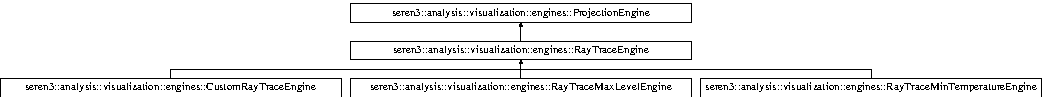
\includegraphics[height=1.30841cm]{classseren3_1_1analysis_1_1visualization_1_1engines_1_1RayTraceEngine}
\end{center}
\end{figure}
\subsection*{Public Member Functions}
\begin{DoxyCompactItemize}
\item 
def \hyperlink{classseren3_1_1analysis_1_1visualization_1_1engines_1_1RayTraceEngine_ab8058104b78f72e69896142942a4a964}{\_\-\_\-init\_\-\_\-}
\item 
\hypertarget{classseren3_1_1analysis_1_1visualization_1_1engines_1_1RayTraceEngine_ae53837d5220069e5c96526e86ceae61f}{
def {\bfseries is\_\-map\_\-engine\_\-for}}
\label{classseren3_1_1analysis_1_1visualization_1_1engines_1_1RayTraceEngine_ae53837d5220069e5c96526e86ceae61f}

\item 
\hypertarget{classseren3_1_1analysis_1_1visualization_1_1engines_1_1RayTraceEngine_a5244189f9a126c0cffaf977b4be79c71}{
def {\bfseries get\_\-process}}
\label{classseren3_1_1analysis_1_1visualization_1_1engines_1_1RayTraceEngine_a5244189f9a126c0cffaf977b4be79c71}

\item 
def \hyperlink{classseren3_1_1analysis_1_1visualization_1_1engines_1_1RayTraceEngine_adaa78a86d554d76c6fd6063453b18d82}{IsMaxAlos}
\end{DoxyCompactItemize}


\subsection{Member Function Documentation}
\hypertarget{classseren3_1_1analysis_1_1visualization_1_1engines_1_1RayTraceEngine_ab8058104b78f72e69896142942a4a964}{
\index{seren3::analysis::visualization::engines::RayTraceEngine@{seren3::analysis::visualization::engines::RayTraceEngine}!\_\-\_\-init\_\-\_\-@{\_\-\_\-init\_\-\_\-}}
\index{\_\-\_\-init\_\-\_\-@{\_\-\_\-init\_\-\_\-}!seren3::analysis::visualization::engines::RayTraceEngine@{seren3::analysis::visualization::engines::RayTraceEngine}}
\subsubsection[{\_\-\_\-init\_\-\_\-}]{\setlength{\rightskip}{0pt plus 5cm}def seren3::analysis::visualization::engines::RayTraceEngine::\_\-\_\-init\_\-\_\- ( {\em self}, \/   {\em family}, \/   {\em field})}}
\label{classseren3_1_1analysis_1_1visualization_1_1engines_1_1RayTraceEngine_ab8058104b78f72e69896142942a4a964}
\begin{DoxyVerb}
    Base class for collecting necessary information to make visualizations of quantities
\end{DoxyVerb}
 

Reimplemented from \hyperlink{classseren3_1_1analysis_1_1visualization_1_1engines_1_1ProjectionEngine_ab9066571de775d34e0a244225a4351fb}{seren3::analysis::visualization::engines::ProjectionEngine}.\hypertarget{classseren3_1_1analysis_1_1visualization_1_1engines_1_1RayTraceEngine_adaa78a86d554d76c6fd6063453b18d82}{
\index{seren3::analysis::visualization::engines::RayTraceEngine@{seren3::analysis::visualization::engines::RayTraceEngine}!IsMaxAlos@{IsMaxAlos}}
\index{IsMaxAlos@{IsMaxAlos}!seren3::analysis::visualization::engines::RayTraceEngine@{seren3::analysis::visualization::engines::RayTraceEngine}}
\subsubsection[{IsMaxAlos}]{\setlength{\rightskip}{0pt plus 5cm}def seren3::analysis::visualization::engines::RayTraceEngine::IsMaxAlos ( {\em self})}}
\label{classseren3_1_1analysis_1_1visualization_1_1engines_1_1RayTraceEngine_adaa78a86d554d76c6fd6063453b18d82}
\begin{DoxyVerb}
True for raytracers
\end{DoxyVerb}
 

Reimplemented from \hyperlink{classseren3_1_1analysis_1_1visualization_1_1engines_1_1ProjectionEngine}{seren3::analysis::visualization::engines::ProjectionEngine}.

The documentation for this class was generated from the following file:\begin{DoxyCompactItemize}
\item 
analysis/visualization/engines.py\end{DoxyCompactItemize}

\hypertarget{classseren3_1_1analysis_1_1visualization_1_1engines_1_1RayTraceMaxLevelEngine}{
\section{seren3::analysis::visualization::engines::RayTraceMaxLevelEngine Class Reference}
\label{classseren3_1_1analysis_1_1visualization_1_1engines_1_1RayTraceMaxLevelEngine}\index{seren3::analysis::visualization::engines::RayTraceMaxLevelEngine@{seren3::analysis::visualization::engines::RayTraceMaxLevelEngine}}
}
Inheritance diagram for seren3::analysis::visualization::engines::RayTraceMaxLevelEngine::\begin{figure}[H]
\begin{center}
\leavevmode
\includegraphics[height=3cm]{classseren3_1_1analysis_1_1visualization_1_1engines_1_1RayTraceMaxLevelEngine}
\end{center}
\end{figure}
\subsection*{Public Member Functions}
\begin{DoxyCompactItemize}
\item 
\hypertarget{classseren3_1_1analysis_1_1visualization_1_1engines_1_1RayTraceMaxLevelEngine_ac9f70fa12d8e23a8906aebfdcbd632e5}{
def {\bfseries \_\-\_\-init\_\-\_\-}}
\label{classseren3_1_1analysis_1_1visualization_1_1engines_1_1RayTraceMaxLevelEngine_ac9f70fa12d8e23a8906aebfdcbd632e5}

\item 
\hypertarget{classseren3_1_1analysis_1_1visualization_1_1engines_1_1RayTraceMaxLevelEngine_a7dfbabd034740bc79a45e8e3d29eef84}{
def {\bfseries is\_\-map\_\-engine\_\-for}}
\label{classseren3_1_1analysis_1_1visualization_1_1engines_1_1RayTraceMaxLevelEngine_a7dfbabd034740bc79a45e8e3d29eef84}

\item 
def \hyperlink{classseren3_1_1analysis_1_1visualization_1_1engines_1_1RayTraceMaxLevelEngine_ae614bc68c2ab9d2a68e8392175fc19e2}{get\_\-map\_\-unit}
\item 
\hypertarget{classseren3_1_1analysis_1_1visualization_1_1engines_1_1RayTraceMaxLevelEngine_ae5f4b238a75add616b828196eadebd07}{
def {\bfseries get\_\-source}}
\label{classseren3_1_1analysis_1_1visualization_1_1engines_1_1RayTraceMaxLevelEngine_ae5f4b238a75add616b828196eadebd07}

\item 
def \hyperlink{classseren3_1_1analysis_1_1visualization_1_1engines_1_1RayTraceMaxLevelEngine_a18ccb6602ed9e6ba18cbff8de2e6ad8c}{get\_\-operator}
\end{DoxyCompactItemize}


\subsection{Member Function Documentation}
\hypertarget{classseren3_1_1analysis_1_1visualization_1_1engines_1_1RayTraceMaxLevelEngine_ae614bc68c2ab9d2a68e8392175fc19e2}{
\index{seren3::analysis::visualization::engines::RayTraceMaxLevelEngine@{seren3::analysis::visualization::engines::RayTraceMaxLevelEngine}!get\_\-map\_\-unit@{get\_\-map\_\-unit}}
\index{get\_\-map\_\-unit@{get\_\-map\_\-unit}!seren3::analysis::visualization::engines::RayTraceMaxLevelEngine@{seren3::analysis::visualization::engines::RayTraceMaxLevelEngine}}
\subsubsection[{get\_\-map\_\-unit}]{\setlength{\rightskip}{0pt plus 5cm}def seren3::analysis::visualization::engines::RayTraceMaxLevelEngine::get\_\-map\_\-unit ( {\em self})}}
\label{classseren3_1_1analysis_1_1visualization_1_1engines_1_1RayTraceMaxLevelEngine_ae614bc68c2ab9d2a68e8392175fc19e2}
\begin{DoxyVerb}
Returns the correct unit for this field
\end{DoxyVerb}
 

Reimplemented from \hyperlink{classseren3_1_1analysis_1_1visualization_1_1engines_1_1ProjectionEngine_a2009db840c6f340e3c39d21dc81a3b77}{seren3::analysis::visualization::engines::ProjectionEngine}.\hypertarget{classseren3_1_1analysis_1_1visualization_1_1engines_1_1RayTraceMaxLevelEngine_a18ccb6602ed9e6ba18cbff8de2e6ad8c}{
\index{seren3::analysis::visualization::engines::RayTraceMaxLevelEngine@{seren3::analysis::visualization::engines::RayTraceMaxLevelEngine}!get\_\-operator@{get\_\-operator}}
\index{get\_\-operator@{get\_\-operator}!seren3::analysis::visualization::engines::RayTraceMaxLevelEngine@{seren3::analysis::visualization::engines::RayTraceMaxLevelEngine}}
\subsubsection[{get\_\-operator}]{\setlength{\rightskip}{0pt plus 5cm}def seren3::analysis::visualization::engines::RayTraceMaxLevelEngine::get\_\-operator ( {\em self})}}
\label{classseren3_1_1analysis_1_1visualization_1_1engines_1_1RayTraceMaxLevelEngine_a18ccb6602ed9e6ba18cbff8de2e6ad8c}
\begin{DoxyVerb}
Return a simple scalar operator for this field, provided it is intensive
\end{DoxyVerb}
 

Reimplemented from \hyperlink{classseren3_1_1analysis_1_1visualization_1_1engines_1_1ProjectionEngine_a42f12a0ccc166799a59549d9fe672f2b}{seren3::analysis::visualization::engines::ProjectionEngine}.

The documentation for this class was generated from the following file:\begin{DoxyCompactItemize}
\item 
analysis/visualization/engines.py\end{DoxyCompactItemize}

\hypertarget{classseren3_1_1analysis_1_1visualization_1_1engines_1_1RayTraceMinTemperatureEngine}{
\section{seren3::analysis::visualization::engines::RayTraceMinTemperatureEngine Class Reference}
\label{classseren3_1_1analysis_1_1visualization_1_1engines_1_1RayTraceMinTemperatureEngine}\index{seren3::analysis::visualization::engines::RayTraceMinTemperatureEngine@{seren3::analysis::visualization::engines::RayTraceMinTemperatureEngine}}
}
Inheritance diagram for seren3::analysis::visualization::engines::RayTraceMinTemperatureEngine::\begin{figure}[H]
\begin{center}
\leavevmode
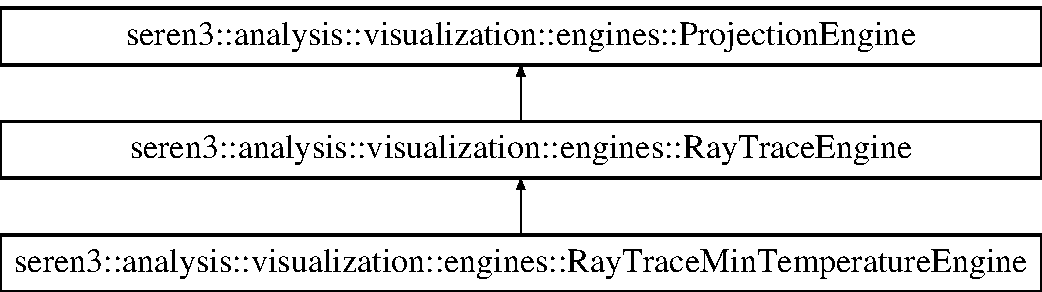
\includegraphics[height=3cm]{classseren3_1_1analysis_1_1visualization_1_1engines_1_1RayTraceMinTemperatureEngine}
\end{center}
\end{figure}
\subsection*{Public Member Functions}
\begin{DoxyCompactItemize}
\item 
\hypertarget{classseren3_1_1analysis_1_1visualization_1_1engines_1_1RayTraceMinTemperatureEngine_ae3ad3045b6e11e034e7b1de487d62b72}{
def {\bfseries \_\-\_\-init\_\-\_\-}}
\label{classseren3_1_1analysis_1_1visualization_1_1engines_1_1RayTraceMinTemperatureEngine_ae3ad3045b6e11e034e7b1de487d62b72}

\item 
\hypertarget{classseren3_1_1analysis_1_1visualization_1_1engines_1_1RayTraceMinTemperatureEngine_a113275fa9fdb58977b93e260f0594454}{
def {\bfseries is\_\-map\_\-engine\_\-for}}
\label{classseren3_1_1analysis_1_1visualization_1_1engines_1_1RayTraceMinTemperatureEngine_a113275fa9fdb58977b93e260f0594454}

\item 
def \hyperlink{classseren3_1_1analysis_1_1visualization_1_1engines_1_1RayTraceMinTemperatureEngine_ae0cd2459819fa5df91728a1a74e91f45}{get\_\-map\_\-unit}
\item 
def \hyperlink{classseren3_1_1analysis_1_1visualization_1_1engines_1_1RayTraceMinTemperatureEngine_aec7ecf391ca54f86f96c840f62785a8e}{get\_\-operator}
\end{DoxyCompactItemize}


\subsection{Detailed Description}
\begin{DoxyVerb}
Computes the minimum temperature along each ray
\end{DoxyVerb}
 

\subsection{Member Function Documentation}
\hypertarget{classseren3_1_1analysis_1_1visualization_1_1engines_1_1RayTraceMinTemperatureEngine_ae0cd2459819fa5df91728a1a74e91f45}{
\index{seren3::analysis::visualization::engines::RayTraceMinTemperatureEngine@{seren3::analysis::visualization::engines::RayTraceMinTemperatureEngine}!get\_\-map\_\-unit@{get\_\-map\_\-unit}}
\index{get\_\-map\_\-unit@{get\_\-map\_\-unit}!seren3::analysis::visualization::engines::RayTraceMinTemperatureEngine@{seren3::analysis::visualization::engines::RayTraceMinTemperatureEngine}}
\subsubsection[{get\_\-map\_\-unit}]{\setlength{\rightskip}{0pt plus 5cm}def seren3::analysis::visualization::engines::RayTraceMinTemperatureEngine::get\_\-map\_\-unit ( {\em self})}}
\label{classseren3_1_1analysis_1_1visualization_1_1engines_1_1RayTraceMinTemperatureEngine_ae0cd2459819fa5df91728a1a74e91f45}
\begin{DoxyVerb}
Returns the correct unit for this field
\end{DoxyVerb}
 

Reimplemented from \hyperlink{classseren3_1_1analysis_1_1visualization_1_1engines_1_1ProjectionEngine_a2009db840c6f340e3c39d21dc81a3b77}{seren3::analysis::visualization::engines::ProjectionEngine}.\hypertarget{classseren3_1_1analysis_1_1visualization_1_1engines_1_1RayTraceMinTemperatureEngine_aec7ecf391ca54f86f96c840f62785a8e}{
\index{seren3::analysis::visualization::engines::RayTraceMinTemperatureEngine@{seren3::analysis::visualization::engines::RayTraceMinTemperatureEngine}!get\_\-operator@{get\_\-operator}}
\index{get\_\-operator@{get\_\-operator}!seren3::analysis::visualization::engines::RayTraceMinTemperatureEngine@{seren3::analysis::visualization::engines::RayTraceMinTemperatureEngine}}
\subsubsection[{get\_\-operator}]{\setlength{\rightskip}{0pt plus 5cm}def seren3::analysis::visualization::engines::RayTraceMinTemperatureEngine::get\_\-operator ( {\em self})}}
\label{classseren3_1_1analysis_1_1visualization_1_1engines_1_1RayTraceMinTemperatureEngine_aec7ecf391ca54f86f96c840f62785a8e}
\begin{DoxyVerb}
Return a simple scalar operator for this field, provided it is intensive
\end{DoxyVerb}
 

Reimplemented from \hyperlink{classseren3_1_1analysis_1_1visualization_1_1engines_1_1ProjectionEngine_a42f12a0ccc166799a59549d9fe672f2b}{seren3::analysis::visualization::engines::ProjectionEngine}.

The documentation for this class was generated from the following file:\begin{DoxyCompactItemize}
\item 
analysis/visualization/engines.py\end{DoxyCompactItemize}

\hypertarget{classseren3_1_1cosmology_1_1power__spectrum_1_1Realisation}{
\section{seren3::cosmology::power\_\-spectrum::Realisation Class Reference}
\label{classseren3_1_1cosmology_1_1power__spectrum_1_1Realisation}\index{seren3::cosmology::power\_\-spectrum::Realisation@{seren3::cosmology::power\_\-spectrum::Realisation}}
}
\subsection*{Public Member Functions}
\begin{DoxyCompactItemize}
\item 
def \hyperlink{classseren3_1_1cosmology_1_1power__spectrum_1_1Realisation_a66657479f264e864519470d5cca27da3}{\_\-\_\-init\_\-\_\-}
\item 
def \hyperlink{classseren3_1_1cosmology_1_1power__spectrum_1_1Realisation_a70cae5b4e147c06dda4f195bf11876a2}{set\_\-fft\_\-sample\_\-spacing}
\item 
def \hyperlink{classseren3_1_1cosmology_1_1power__spectrum_1_1Realisation_a2d7f743d7a8bad924187e6f9fe379417}{realise\_\-density}
\item 
def \hyperlink{classseren3_1_1cosmology_1_1power__spectrum_1_1Realisation_a0e1f42e5de6f6d530735c8fe79529dd1}{realise\_\-velocity}
\item 
def \hyperlink{classseren3_1_1cosmology_1_1power__spectrum_1_1Realisation_a9ba2161fc48fe4a8588f84e62e668dc0}{apply\_\-bias}
\item 
def \hyperlink{classseren3_1_1cosmology_1_1power__spectrum_1_1Realisation_ae1949bbd25d64f3e15751e4f78bf845d}{window}
\item 
def \hyperlink{classseren3_1_1cosmology_1_1power__spectrum_1_1Realisation_aba11124fa5b26227a07e4daa0413405a}{window1}
\item 
def \hyperlink{classseren3_1_1cosmology_1_1power__spectrum_1_1Realisation_a7aa3738c4f9874c56702655c77463f98}{sigmaR}
\item 
def \hyperlink{classseren3_1_1cosmology_1_1power__spectrum_1_1Realisation_a11401db5e3772aed682363e17a0bf8d8}{sigma8}
\item 
def \hyperlink{classseren3_1_1cosmology_1_1power__spectrum_1_1Realisation_a2ae0cbfd6b3781bf57b2b89188fc7cad}{binned\_\-power\_\-spectrum}
\item 
def \hyperlink{classseren3_1_1cosmology_1_1power__spectrum_1_1Realisation_a02f12b743f326436bd4b9a482e6f0596}{theoretical\_\-power\_\-spectrum}
\item 
def \hyperlink{classseren3_1_1cosmology_1_1power__spectrum_1_1Realisation_a5db10734093eab1e21e2e1162375ec65}{test\_\-sampling\_\-error}
\item 
def \hyperlink{classseren3_1_1cosmology_1_1power__spectrum_1_1Realisation_a3fa53f286013d68966617cb9b360e4bf}{test\_\-parseval}
\item 
\hypertarget{classseren3_1_1cosmology_1_1power__spectrum_1_1Realisation_a7ff9f2220ce9615f30667a7b49935a88}{
def {\bfseries test}}
\label{classseren3_1_1cosmology_1_1power__spectrum_1_1Realisation_a7ff9f2220ce9615f30667a7b49935a88}

\end{DoxyCompactItemize}
\subsection*{Public Attributes}
\begin{DoxyCompactItemize}
\item 
\hypertarget{classseren3_1_1cosmology_1_1power__spectrum_1_1Realisation_a2ef4114865b0824078d357ad107efff5}{
{\bfseries cosmo}}
\label{classseren3_1_1cosmology_1_1power__spectrum_1_1Realisation_a2ef4114865b0824078d357ad107efff5}

\item 
\hypertarget{classseren3_1_1cosmology_1_1power__spectrum_1_1Realisation_a391bdcfa7f8f75296b022a1eef69b7ac}{
{\bfseries x}}
\label{classseren3_1_1cosmology_1_1power__spectrum_1_1Realisation_a391bdcfa7f8f75296b022a1eef69b7ac}

\item 
\hypertarget{classseren3_1_1cosmology_1_1power__spectrum_1_1Realisation_a7de9d8598a2810796bb85709c252b756}{
{\bfseries N}}
\label{classseren3_1_1cosmology_1_1power__spectrum_1_1Realisation_a7de9d8598a2810796bb85709c252b756}

\item 
\hypertarget{classseren3_1_1cosmology_1_1power__spectrum_1_1Realisation_a134bca39e4d44196e79a9eb7aa7e901e}{
{\bfseries L}}
\label{classseren3_1_1cosmology_1_1power__spectrum_1_1Realisation_a134bca39e4d44196e79a9eb7aa7e901e}

\item 
\hypertarget{classseren3_1_1cosmology_1_1power__spectrum_1_1Realisation_af6ce836b6c2c34f77a2a9b09d493baa9}{
{\bfseries boxfactor}}
\label{classseren3_1_1cosmology_1_1power__spectrum_1_1Realisation_af6ce836b6c2c34f77a2a9b09d493baa9}

\item 
\hypertarget{classseren3_1_1cosmology_1_1power__spectrum_1_1Realisation_a8d791275546207943faa1c5f1735ebc2}{
{\bfseries kmin}}
\label{classseren3_1_1cosmology_1_1power__spectrum_1_1Realisation_a8d791275546207943faa1c5f1735ebc2}

\item 
\hypertarget{classseren3_1_1cosmology_1_1power__spectrum_1_1Realisation_a088798ddf94a280d491393a7dd237a33}{
{\bfseries kmax}}
\label{classseren3_1_1cosmology_1_1power__spectrum_1_1Realisation_a088798ddf94a280d491393a7dd237a33}

\item 
\hypertarget{classseren3_1_1cosmology_1_1power__spectrum_1_1Realisation_a0a7dfb8709de34c8ebc0fc2df2f1fca4}{
{\bfseries kx}}
\label{classseren3_1_1cosmology_1_1power__spectrum_1_1Realisation_a0a7dfb8709de34c8ebc0fc2df2f1fca4}

\item 
\hypertarget{classseren3_1_1cosmology_1_1power__spectrum_1_1Realisation_a425f7d8794cab01391a8ddd7fb2dd50d}{
{\bfseries ky}}
\label{classseren3_1_1cosmology_1_1power__spectrum_1_1Realisation_a425f7d8794cab01391a8ddd7fb2dd50d}

\item 
\hypertarget{classseren3_1_1cosmology_1_1power__spectrum_1_1Realisation_a35e83c95eff86ba0ef9bed59d6818b84}{
{\bfseries kz}}
\label{classseren3_1_1cosmology_1_1power__spectrum_1_1Realisation_a35e83c95eff86ba0ef9bed59d6818b84}

\item 
\hypertarget{classseren3_1_1cosmology_1_1power__spectrum_1_1Realisation_a069501387fe3416eced6b8e02ac109b8}{
{\bfseries k}}
\label{classseren3_1_1cosmology_1_1power__spectrum_1_1Realisation_a069501387fe3416eced6b8e02ac109b8}

\item 
\hypertarget{classseren3_1_1cosmology_1_1power__spectrum_1_1Realisation_aad2c15ec18f969a0a98d0b5553620921}{
{\bfseries delta\_\-k}}
\label{classseren3_1_1cosmology_1_1power__spectrum_1_1Realisation_aad2c15ec18f969a0a98d0b5553620921}

\item 
\hypertarget{classseren3_1_1cosmology_1_1power__spectrum_1_1Realisation_a18d623ea9f0cfa3e02982d907351b159}{
{\bfseries delta\_\-x}}
\label{classseren3_1_1cosmology_1_1power__spectrum_1_1Realisation_a18d623ea9f0cfa3e02982d907351b159}

\end{DoxyCompactItemize}


\subsection{Member Function Documentation}
\hypertarget{classseren3_1_1cosmology_1_1power__spectrum_1_1Realisation_a66657479f264e864519470d5cca27da3}{
\index{seren3::cosmology::power\_\-spectrum::Realisation@{seren3::cosmology::power\_\-spectrum::Realisation}!\_\-\_\-init\_\-\_\-@{\_\-\_\-init\_\-\_\-}}
\index{\_\-\_\-init\_\-\_\-@{\_\-\_\-init\_\-\_\-}!seren3::cosmology::power_spectrum::Realisation@{seren3::cosmology::power\_\-spectrum::Realisation}}
\subsubsection[{\_\-\_\-init\_\-\_\-}]{\setlength{\rightskip}{0pt plus 5cm}def seren3::cosmology::power\_\-spectrum::Realisation::\_\-\_\-init\_\-\_\- ( {\em self}, \/   {\em cosmo} = {\ttfamily DEFAULT\_\-COSMOLOGY}, \/   {\em scale} = {\ttfamily 0.2}, \/   {\em nsamp} = {\ttfamily 128}, \/   {\em filename} = {\ttfamily None}, \/   {\em cols} = {\ttfamily None})}}
\label{classseren3_1_1cosmology_1_1power__spectrum_1_1Realisation_a66657479f264e864519470d5cca27da3}
\begin{DoxyVerb}Initialise a 3D box with matter distribution described by a given power spectrum.
Parameters:
    scale (float): Boxsize (Mpc)
    nsamp (int): Number of cells per dimension
\end{DoxyVerb}
 \hypertarget{classseren3_1_1cosmology_1_1power__spectrum_1_1Realisation_a9ba2161fc48fe4a8588f84e62e668dc0}{
\index{seren3::cosmology::power\_\-spectrum::Realisation@{seren3::cosmology::power\_\-spectrum::Realisation}!apply\_\-bias@{apply\_\-bias}}
\index{apply\_\-bias@{apply\_\-bias}!seren3::cosmology::power_spectrum::Realisation@{seren3::cosmology::power\_\-spectrum::Realisation}}
\subsubsection[{apply\_\-bias}]{\setlength{\rightskip}{0pt plus 5cm}def seren3::cosmology::power\_\-spectrum::Realisation::apply\_\-bias ( {\em self}, \/   {\em k\_\-b}, \/   {\em b})}}
\label{classseren3_1_1cosmology_1_1power__spectrum_1_1Realisation_a9ba2161fc48fe4a8588f84e62e668dc0}
\begin{DoxyVerb}Apply a bias to the realisations power spectrum, and recompute the 3D field.
Parameters:
    b (array): bias to deconvolve with the delta_x field, such that:
    delta_x = ifft(delta_k/b)
\end{DoxyVerb}
 \hypertarget{classseren3_1_1cosmology_1_1power__spectrum_1_1Realisation_a2ae0cbfd6b3781bf57b2b89188fc7cad}{
\index{seren3::cosmology::power\_\-spectrum::Realisation@{seren3::cosmology::power\_\-spectrum::Realisation}!binned\_\-power\_\-spectrum@{binned\_\-power\_\-spectrum}}
\index{binned\_\-power\_\-spectrum@{binned\_\-power\_\-spectrum}!seren3::cosmology::power_spectrum::Realisation@{seren3::cosmology::power\_\-spectrum::Realisation}}
\subsubsection[{binned\_\-power\_\-spectrum}]{\setlength{\rightskip}{0pt plus 5cm}def seren3::cosmology::power\_\-spectrum::Realisation::binned\_\-power\_\-spectrum ( {\em self}, \/   {\em nbins} = {\ttfamily 20})}}
\label{classseren3_1_1cosmology_1_1power__spectrum_1_1Realisation_a2ae0cbfd6b3781bf57b2b89188fc7cad}
\begin{DoxyVerb}Return a binned power spectrum, calculated from the realisation.\end{DoxyVerb}
 \hypertarget{classseren3_1_1cosmology_1_1power__spectrum_1_1Realisation_a2d7f743d7a8bad924187e6f9fe379417}{
\index{seren3::cosmology::power\_\-spectrum::Realisation@{seren3::cosmology::power\_\-spectrum::Realisation}!realise\_\-density@{realise\_\-density}}
\index{realise\_\-density@{realise\_\-density}!seren3::cosmology::power_spectrum::Realisation@{seren3::cosmology::power\_\-spectrum::Realisation}}
\subsubsection[{realise\_\-density}]{\setlength{\rightskip}{0pt plus 5cm}def seren3::cosmology::power\_\-spectrum::Realisation::realise\_\-density ( {\em self}, \/   {\em filename} = {\ttfamily None}, \/   {\em cols} = {\ttfamily None})}}
\label{classseren3_1_1cosmology_1_1power__spectrum_1_1Realisation_a2d7f743d7a8bad924187e6f9fe379417}
\begin{DoxyVerb}Create realisation of the power spectrum by randomly sampling
from Gaussian distributions of variance P(k) for each k mode.\end{DoxyVerb}
 \hypertarget{classseren3_1_1cosmology_1_1power__spectrum_1_1Realisation_a0e1f42e5de6f6d530735c8fe79529dd1}{
\index{seren3::cosmology::power\_\-spectrum::Realisation@{seren3::cosmology::power\_\-spectrum::Realisation}!realise\_\-velocity@{realise\_\-velocity}}
\index{realise\_\-velocity@{realise\_\-velocity}!seren3::cosmology::power_spectrum::Realisation@{seren3::cosmology::power\_\-spectrum::Realisation}}
\subsubsection[{realise\_\-velocity}]{\setlength{\rightskip}{0pt plus 5cm}def seren3::cosmology::power\_\-spectrum::Realisation::realise\_\-velocity ( {\em self})}}
\label{classseren3_1_1cosmology_1_1power__spectrum_1_1Realisation_a0e1f42e5de6f6d530735c8fe79529dd1}
\begin{DoxyVerb}Realise the (unscaled) velocity field in Fourier space. See 
   Dodelson Eq. 9.18 for an expression; we factor out the 
   time-dependent quantities here. They can be added at a later stage.\end{DoxyVerb}
 \hypertarget{classseren3_1_1cosmology_1_1power__spectrum_1_1Realisation_a70cae5b4e147c06dda4f195bf11876a2}{
\index{seren3::cosmology::power\_\-spectrum::Realisation@{seren3::cosmology::power\_\-spectrum::Realisation}!set\_\-fft\_\-sample\_\-spacing@{set\_\-fft\_\-sample\_\-spacing}}
\index{set\_\-fft\_\-sample\_\-spacing@{set\_\-fft\_\-sample\_\-spacing}!seren3::cosmology::power_spectrum::Realisation@{seren3::cosmology::power\_\-spectrum::Realisation}}
\subsubsection[{set\_\-fft\_\-sample\_\-spacing}]{\setlength{\rightskip}{0pt plus 5cm}def seren3::cosmology::power\_\-spectrum::Realisation::set\_\-fft\_\-sample\_\-spacing ( {\em self})}}
\label{classseren3_1_1cosmology_1_1power__spectrum_1_1Realisation_a70cae5b4e147c06dda4f195bf11876a2}
\begin{DoxyVerb}Calculate the sample spacing in Fourier space, given some symmetric 3D 
box in real space, with 1D grid point coordinates 'x'.\end{DoxyVerb}
 \hypertarget{classseren3_1_1cosmology_1_1power__spectrum_1_1Realisation_a11401db5e3772aed682363e17a0bf8d8}{
\index{seren3::cosmology::power\_\-spectrum::Realisation@{seren3::cosmology::power\_\-spectrum::Realisation}!sigma8@{sigma8}}
\index{sigma8@{sigma8}!seren3::cosmology::power_spectrum::Realisation@{seren3::cosmology::power\_\-spectrum::Realisation}}
\subsubsection[{sigma8}]{\setlength{\rightskip}{0pt plus 5cm}def seren3::cosmology::power\_\-spectrum::Realisation::sigma8 ( {\em self})}}
\label{classseren3_1_1cosmology_1_1power__spectrum_1_1Realisation_a11401db5e3772aed682363e17a0bf8d8}
\begin{DoxyVerb}Get variance of matter perturbations on smoothing scale of 
   8 h^-1 Mpc.\end{DoxyVerb}
 \hypertarget{classseren3_1_1cosmology_1_1power__spectrum_1_1Realisation_a7aa3738c4f9874c56702655c77463f98}{
\index{seren3::cosmology::power\_\-spectrum::Realisation@{seren3::cosmology::power\_\-spectrum::Realisation}!sigmaR@{sigmaR}}
\index{sigmaR@{sigmaR}!seren3::cosmology::power_spectrum::Realisation@{seren3::cosmology::power\_\-spectrum::Realisation}}
\subsubsection[{sigmaR}]{\setlength{\rightskip}{0pt plus 5cm}def seren3::cosmology::power\_\-spectrum::Realisation::sigmaR ( {\em self}, \/   {\em R})}}
\label{classseren3_1_1cosmology_1_1power__spectrum_1_1Realisation_a7aa3738c4f9874c56702655c77463f98}
\begin{DoxyVerb}Get variance of matter perturbations, smoothed with a tophat filter 
   of radius R h^-1 Mpc.\end{DoxyVerb}
 \hypertarget{classseren3_1_1cosmology_1_1power__spectrum_1_1Realisation_a3fa53f286013d68966617cb9b360e4bf}{
\index{seren3::cosmology::power\_\-spectrum::Realisation@{seren3::cosmology::power\_\-spectrum::Realisation}!test\_\-parseval@{test\_\-parseval}}
\index{test\_\-parseval@{test\_\-parseval}!seren3::cosmology::power_spectrum::Realisation@{seren3::cosmology::power\_\-spectrum::Realisation}}
\subsubsection[{test\_\-parseval}]{\setlength{\rightskip}{0pt plus 5cm}def seren3::cosmology::power\_\-spectrum::Realisation::test\_\-parseval ( {\em self})}}
\label{classseren3_1_1cosmology_1_1power__spectrum_1_1Realisation_a3fa53f286013d68966617cb9b360e4bf}
\begin{DoxyVerb}Ensure that Parseval's theorem is satisfied for delta_x and delta_k, 
   i.e. <delta_x^2> = Sum_k[P(k)]. Important consistency check for FT;
   should return unity if everything is OK.
\end{DoxyVerb}
 \hypertarget{classseren3_1_1cosmology_1_1power__spectrum_1_1Realisation_a5db10734093eab1e21e2e1162375ec65}{
\index{seren3::cosmology::power\_\-spectrum::Realisation@{seren3::cosmology::power\_\-spectrum::Realisation}!test\_\-sampling\_\-error@{test\_\-sampling\_\-error}}
\index{test\_\-sampling\_\-error@{test\_\-sampling\_\-error}!seren3::cosmology::power_spectrum::Realisation@{seren3::cosmology::power\_\-spectrum::Realisation}}
\subsubsection[{test\_\-sampling\_\-error}]{\setlength{\rightskip}{0pt plus 5cm}def seren3::cosmology::power\_\-spectrum::Realisation::test\_\-sampling\_\-error ( {\em self})}}
\label{classseren3_1_1cosmology_1_1power__spectrum_1_1Realisation_a5db10734093eab1e21e2e1162375ec65}
\begin{DoxyVerb}P(k) is sampled within some finite window in the interval 
   [kmin, kmax], where kmin=2pi/L and kmax=2pi*sqrt(3)*(N/2)*(1/L) 
   (for 3D FT). The lack of sampling in some regions of k-space means 
   that sigma8 can't be perfectly reconstructed (see U-L. Pen, 
   arXiv:astro-ph/9709261 for a discussion).
   This function calculates sigma8 from the realised box, and compares 
   this with the theoretical calculation for sigma8 over a large 
   k-window, and over a k-window of the same size as for the box.
\end{DoxyVerb}
 \hypertarget{classseren3_1_1cosmology_1_1power__spectrum_1_1Realisation_a02f12b743f326436bd4b9a482e6f0596}{
\index{seren3::cosmology::power\_\-spectrum::Realisation@{seren3::cosmology::power\_\-spectrum::Realisation}!theoretical\_\-power\_\-spectrum@{theoretical\_\-power\_\-spectrum}}
\index{theoretical\_\-power\_\-spectrum@{theoretical\_\-power\_\-spectrum}!seren3::cosmology::power_spectrum::Realisation@{seren3::cosmology::power\_\-spectrum::Realisation}}
\subsubsection[{theoretical\_\-power\_\-spectrum}]{\setlength{\rightskip}{0pt plus 5cm}def seren3::cosmology::power\_\-spectrum::Realisation::theoretical\_\-power\_\-spectrum ( {\em self})}}
\label{classseren3_1_1cosmology_1_1power__spectrum_1_1Realisation_a02f12b743f326436bd4b9a482e6f0596}
\begin{DoxyVerb}Calculate the theoretical power spectrum for the given cosmological 
   parameters, using Cosmolopy. Does not depend on the realisation.\end{DoxyVerb}
 \hypertarget{classseren3_1_1cosmology_1_1power__spectrum_1_1Realisation_ae1949bbd25d64f3e15751e4f78bf845d}{
\index{seren3::cosmology::power\_\-spectrum::Realisation@{seren3::cosmology::power\_\-spectrum::Realisation}!window@{window}}
\index{window@{window}!seren3::cosmology::power_spectrum::Realisation@{seren3::cosmology::power\_\-spectrum::Realisation}}
\subsubsection[{window}]{\setlength{\rightskip}{0pt plus 5cm}def seren3::cosmology::power\_\-spectrum::Realisation::window ( {\em self}, \/   {\em k}, \/   {\em R})}}
\label{classseren3_1_1cosmology_1_1power__spectrum_1_1Realisation_ae1949bbd25d64f3e15751e4f78bf845d}
\begin{DoxyVerb}Fourier transform of tophat window function, used to calculate 
   sigmaR etc. See "Cosmology", S. Weinberg, Eq.8.1.46.\end{DoxyVerb}
 \hypertarget{classseren3_1_1cosmology_1_1power__spectrum_1_1Realisation_aba11124fa5b26227a07e4daa0413405a}{
\index{seren3::cosmology::power\_\-spectrum::Realisation@{seren3::cosmology::power\_\-spectrum::Realisation}!window1@{window1}}
\index{window1@{window1}!seren3::cosmology::power_spectrum::Realisation@{seren3::cosmology::power\_\-spectrum::Realisation}}
\subsubsection[{window1}]{\setlength{\rightskip}{0pt plus 5cm}def seren3::cosmology::power\_\-spectrum::Realisation::window1 ( {\em self}, \/   {\em k}, \/   {\em R})}}
\label{classseren3_1_1cosmology_1_1power__spectrum_1_1Realisation_aba11124fa5b26227a07e4daa0413405a}
\begin{DoxyVerb}Fourier transform of tophat window function, used to calculate 
   sigmaR etc. See "Cosmology", S. Weinberg, Eq.8.1.46.\end{DoxyVerb}
 

The documentation for this class was generated from the following file:\begin{DoxyCompactItemize}
\item 
cosmology/power\_\-spectrum.py\end{DoxyCompactItemize}

\hypertarget{classseren3_1_1array_1_1RemoteKeyboardInterrupt}{
\section{seren3::array::RemoteKeyboardInterrupt Class Reference}
\label{classseren3_1_1array_1_1RemoteKeyboardInterrupt}\index{seren3::array::RemoteKeyboardInterrupt@{seren3::array::RemoteKeyboardInterrupt}}
}
\subsection*{Public Member Functions}
\begin{DoxyCompactItemize}
\item 
def \hyperlink{classseren3_1_1array_1_1RemoteKeyboardInterrupt_a465c9a54d5b8b38699014c9d4dca8b35}{shared\_\-array\_\-remote}
\item 
def \hyperlink{classseren3_1_1array_1_1RemoteKeyboardInterrupt_aff7e4bd891bea9300aa525620a14e490}{remote\_\-map}
\item 
def \hyperlink{classseren3_1_1array_1_1RemoteKeyboardInterrupt_a07c542d0d324f612b172cee29290c4f3}{exit\_\-cleanup}
\end{DoxyCompactItemize}


\subsection{Member Function Documentation}
\hypertarget{classseren3_1_1array_1_1RemoteKeyboardInterrupt_a07c542d0d324f612b172cee29290c4f3}{
\index{seren3::array::RemoteKeyboardInterrupt@{seren3::array::RemoteKeyboardInterrupt}!exit\_\-cleanup@{exit\_\-cleanup}}
\index{exit\_\-cleanup@{exit\_\-cleanup}!seren3::array::RemoteKeyboardInterrupt@{seren3::array::RemoteKeyboardInterrupt}}
\subsubsection[{exit\_\-cleanup}]{\setlength{\rightskip}{0pt plus 5cm}def seren3::array::RemoteKeyboardInterrupt::exit\_\-cleanup ()}}
\label{classseren3_1_1array_1_1RemoteKeyboardInterrupt_a07c542d0d324f612b172cee29290c4f3}
\begin{DoxyVerb}Clean up any shared memory that has not yet been freed. In
theory this should not be required, but it is here as a safety
net.\end{DoxyVerb}
 \hypertarget{classseren3_1_1array_1_1RemoteKeyboardInterrupt_aff7e4bd891bea9300aa525620a14e490}{
\index{seren3::array::RemoteKeyboardInterrupt@{seren3::array::RemoteKeyboardInterrupt}!remote\_\-map@{remote\_\-map}}
\index{remote\_\-map@{remote\_\-map}!seren3::array::RemoteKeyboardInterrupt@{seren3::array::RemoteKeyboardInterrupt}}
\subsubsection[{remote\_\-map}]{\setlength{\rightskip}{0pt plus 5cm}def seren3::array::RemoteKeyboardInterrupt::remote\_\-map ( {\em pool}, \/   {\em fn}, \/   {\em iterables})}}
\label{classseren3_1_1array_1_1RemoteKeyboardInterrupt_aff7e4bd891bea9300aa525620a14e490}
\begin{DoxyVerb}A replacement for python's in-built map function, sending out tasks
to the pool and performing the magic required to transport shared memory arrays
correctly. The function *fn* must be wrapped with the *shared_array_remote*
decorator to interface correctly with this magic.\end{DoxyVerb}
 \hypertarget{classseren3_1_1array_1_1RemoteKeyboardInterrupt_a465c9a54d5b8b38699014c9d4dca8b35}{
\index{seren3::array::RemoteKeyboardInterrupt@{seren3::array::RemoteKeyboardInterrupt}!shared\_\-array\_\-remote@{shared\_\-array\_\-remote}}
\index{shared\_\-array\_\-remote@{shared\_\-array\_\-remote}!seren3::array::RemoteKeyboardInterrupt@{seren3::array::RemoteKeyboardInterrupt}}
\subsubsection[{shared\_\-array\_\-remote}]{\setlength{\rightskip}{0pt plus 5cm}def seren3::array::RemoteKeyboardInterrupt::shared\_\-array\_\-remote ( {\em fn})}}
\label{classseren3_1_1array_1_1RemoteKeyboardInterrupt_a465c9a54d5b8b38699014c9d4dca8b35}
\begin{DoxyVerb}A decorator for functions returning a new function that is
suitable for use remotely. Inputs to and outputs from the function
can be transferred efficiently if they are backed onto shared
memory. Ownership of any shared memory returned by the function
is transferred.\end{DoxyVerb}
 

The documentation for this class was generated from the following file:\begin{DoxyCompactItemize}
\item 
array.py\end{DoxyCompactItemize}

\hypertarget{classseren3_1_1analysis_1_1parallel_1_1mpi_1_1Result}{
\section{seren3::analysis::parallel::mpi::Result Class Reference}
\label{classseren3_1_1analysis_1_1parallel_1_1mpi_1_1Result}\index{seren3::analysis::parallel::mpi::Result@{seren3::analysis::parallel::mpi::Result}}
}
\subsection*{Public Member Functions}
\begin{DoxyCompactItemize}
\item 
\hypertarget{classseren3_1_1analysis_1_1parallel_1_1mpi_1_1Result_a64b5638b66017645c42bec256dd58f95}{
def {\bfseries \_\-\_\-init\_\-\_\-}}
\label{classseren3_1_1analysis_1_1parallel_1_1mpi_1_1Result_a64b5638b66017645c42bec256dd58f95}

\item 
\hypertarget{classseren3_1_1analysis_1_1parallel_1_1mpi_1_1Result_a4346441d71dc534b42498544faee00a3}{
def {\bfseries \_\-\_\-repr\_\-\_\-}}
\label{classseren3_1_1analysis_1_1parallel_1_1mpi_1_1Result_a4346441d71dc534b42498544faee00a3}

\item 
\hypertarget{classseren3_1_1analysis_1_1parallel_1_1mpi_1_1Result_af7862b9dc29c5dc30482f04372ea1dc1}{
def {\bfseries \_\-\_\-eq\_\-\_\-}}
\label{classseren3_1_1analysis_1_1parallel_1_1mpi_1_1Result_af7862b9dc29c5dc30482f04372ea1dc1}

\item 
\hypertarget{classseren3_1_1analysis_1_1parallel_1_1mpi_1_1Result_a74d8ab0902d414aa7d9ce3b7055b67a0}{
def {\bfseries \_\-\_\-ne\_\-\_\-}}
\label{classseren3_1_1analysis_1_1parallel_1_1mpi_1_1Result_a74d8ab0902d414aa7d9ce3b7055b67a0}

\item 
\hypertarget{classseren3_1_1analysis_1_1parallel_1_1mpi_1_1Result_a1f79badced6558a563c7d1090070a05c}{
def {\bfseries \_\-\_\-hash\_\-\_\-}}
\label{classseren3_1_1analysis_1_1parallel_1_1mpi_1_1Result_a1f79badced6558a563c7d1090070a05c}

\end{DoxyCompactItemize}
\subsection*{Public Attributes}
\begin{DoxyCompactItemize}
\item 
\hypertarget{classseren3_1_1analysis_1_1parallel_1_1mpi_1_1Result_a5091dadf2d89ac97f1c9b0fd8b9a677f}{
{\bfseries rank}}
\label{classseren3_1_1analysis_1_1parallel_1_1mpi_1_1Result_a5091dadf2d89ac97f1c9b0fd8b9a677f}

\item 
\hypertarget{classseren3_1_1analysis_1_1parallel_1_1mpi_1_1Result_ad0cde82892ef6455c869ad2a2c5f0977}{
{\bfseries idx}}
\label{classseren3_1_1analysis_1_1parallel_1_1mpi_1_1Result_ad0cde82892ef6455c869ad2a2c5f0977}

\item 
\hypertarget{classseren3_1_1analysis_1_1parallel_1_1mpi_1_1Result_a4841c4318735311cc4d5bb5aab3f0016}{
{\bfseries result}}
\label{classseren3_1_1analysis_1_1parallel_1_1mpi_1_1Result_a4841c4318735311cc4d5bb5aab3f0016}

\end{DoxyCompactItemize}


\subsection{Detailed Description}
\begin{DoxyVerb}
Simple wrapper object to contain result of single iteration MPI computation
\end{DoxyVerb}
 

The documentation for this class was generated from the following file:\begin{DoxyCompactItemize}
\item 
analysis/parallel/mpi.py\end{DoxyCompactItemize}

\hypertarget{classseren3_1_1analysis_1_1parallel_1_1Result}{
\section{seren3::analysis::parallel::Result Class Reference}
\label{classseren3_1_1analysis_1_1parallel_1_1Result}\index{seren3::analysis::parallel::Result@{seren3::analysis::parallel::Result}}
}
\subsection*{Public Member Functions}
\begin{DoxyCompactItemize}
\item 
\hypertarget{classseren3_1_1analysis_1_1parallel_1_1Result_a1eb0096054b0920660f64ace8b2d0763}{
def {\bfseries \_\-\_\-init\_\-\_\-}}
\label{classseren3_1_1analysis_1_1parallel_1_1Result_a1eb0096054b0920660f64ace8b2d0763}

\item 
\hypertarget{classseren3_1_1analysis_1_1parallel_1_1Result_a26128ac8c9c87f3442e1511344c4ab53}{
def {\bfseries \_\-\_\-repr\_\-\_\-}}
\label{classseren3_1_1analysis_1_1parallel_1_1Result_a26128ac8c9c87f3442e1511344c4ab53}

\item 
\hypertarget{classseren3_1_1analysis_1_1parallel_1_1Result_aa1d431534c797b95e5ebb645d48e0a03}{
def {\bfseries \_\-\_\-eq\_\-\_\-}}
\label{classseren3_1_1analysis_1_1parallel_1_1Result_aa1d431534c797b95e5ebb645d48e0a03}

\item 
\hypertarget{classseren3_1_1analysis_1_1parallel_1_1Result_ac70dee7892ecdabc8b297da01c0ff605}{
def {\bfseries \_\-\_\-ne\_\-\_\-}}
\label{classseren3_1_1analysis_1_1parallel_1_1Result_ac70dee7892ecdabc8b297da01c0ff605}

\item 
\hypertarget{classseren3_1_1analysis_1_1parallel_1_1Result_a2d32419e77779319a4f34dbc9f0860ce}{
def {\bfseries \_\-\_\-hash\_\-\_\-}}
\label{classseren3_1_1analysis_1_1parallel_1_1Result_a2d32419e77779319a4f34dbc9f0860ce}

\end{DoxyCompactItemize}
\subsection*{Public Attributes}
\begin{DoxyCompactItemize}
\item 
\hypertarget{classseren3_1_1analysis_1_1parallel_1_1Result_a3c974b07359552e0239e4fe10369248f}{
{\bfseries rank}}
\label{classseren3_1_1analysis_1_1parallel_1_1Result_a3c974b07359552e0239e4fe10369248f}

\item 
\hypertarget{classseren3_1_1analysis_1_1parallel_1_1Result_a9310810b011d2b934ec720a7172425ae}{
{\bfseries idx}}
\label{classseren3_1_1analysis_1_1parallel_1_1Result_a9310810b011d2b934ec720a7172425ae}

\item 
\hypertarget{classseren3_1_1analysis_1_1parallel_1_1Result_a1a847949fd8b917237b3e085a7ab64eb}{
{\bfseries result}}
\label{classseren3_1_1analysis_1_1parallel_1_1Result_a1a847949fd8b917237b3e085a7ab64eb}

\end{DoxyCompactItemize}


\subsection{Detailed Description}
\begin{DoxyVerb}
Simple wrapper object to contain result of single iteration MPI computation
\end{DoxyVerb}
 

The documentation for this class was generated from the following file:\begin{DoxyCompactItemize}
\item 
analysis/parallel/\_\-\_\-init\_\-\_\-.py\end{DoxyCompactItemize}

\hypertarget{classseren3_1_1halos_1_1halos_1_1RockstarCatalogue}{
\section{seren3::halos::halos::RockstarCatalogue Class Reference}
\label{classseren3_1_1halos_1_1halos_1_1RockstarCatalogue}\index{seren3::halos::halos::RockstarCatalogue@{seren3::halos::halos::RockstarCatalogue}}
}
Inheritance diagram for seren3::halos::halos::RockstarCatalogue::\begin{figure}[H]
\begin{center}
\leavevmode
\includegraphics[height=2cm]{classseren3_1_1halos_1_1halos_1_1RockstarCatalogue}
\end{center}
\end{figure}
\subsection*{Public Member Functions}
\begin{DoxyCompactItemize}
\item 
\hypertarget{classseren3_1_1halos_1_1halos_1_1RockstarCatalogue_a9cc6cc02aaa5b00bb928c258ea77c576}{
def {\bfseries \_\-\_\-init\_\-\_\-}}
\label{classseren3_1_1halos_1_1halos_1_1RockstarCatalogue_a9cc6cc02aaa5b00bb928c258ea77c576}

\item 
\hypertarget{classseren3_1_1halos_1_1halos_1_1RockstarCatalogue_aac709561d206eba20981daeaefc5b238}{
def {\bfseries can\_\-load}}
\label{classseren3_1_1halos_1_1halos_1_1RockstarCatalogue_aac709561d206eba20981daeaefc5b238}

\item 
\hypertarget{classseren3_1_1halos_1_1halos_1_1RockstarCatalogue_aec69313605298331b8c4bccf31afd6e6}{
def {\bfseries get\_\-rockstar\_\-info\_\-fname}}
\label{classseren3_1_1halos_1_1halos_1_1RockstarCatalogue_aec69313605298331b8c4bccf31afd6e6}

\item 
def \hyperlink{classseren3_1_1halos_1_1halos_1_1RockstarCatalogue_ab55aae49df70e416fba591c9682c264b}{get\_\-filename}
\item 
def \hyperlink{classseren3_1_1halos_1_1halos_1_1RockstarCatalogue_a648f766d002674cc441e36260c98b02f}{get\_\-boxsize}
\item 
\hypertarget{classseren3_1_1halos_1_1halos_1_1RockstarCatalogue_a66c4c06bcb33666b7247f6b50bf49b3d}{
def {\bfseries load}}
\label{classseren3_1_1halos_1_1halos_1_1RockstarCatalogue_a66c4c06bcb33666b7247f6b50bf49b3d}

\end{DoxyCompactItemize}
\subsection*{Public Attributes}
\begin{DoxyCompactItemize}
\item 
\hypertarget{classseren3_1_1halos_1_1halos_1_1RockstarCatalogue_a2141d834ef7ccf6d4251f6a5b6bf90b4}{
{\bfseries finder\_\-base\_\-dir}}
\label{classseren3_1_1halos_1_1halos_1_1RockstarCatalogue_a2141d834ef7ccf6d4251f6a5b6bf90b4}

\end{DoxyCompactItemize}
\subsection*{Static Public Attributes}
\begin{DoxyCompactItemize}
\item 
tuple {\bfseries halo\_\-type}
\item 
dictionary {\bfseries units}
\end{DoxyCompactItemize}


\subsection{Detailed Description}
\begin{DoxyVerb}
Class to handle catalogues produced by Rockstar
Reads the out.list files
\end{DoxyVerb}
 

\subsection{Member Function Documentation}
\hypertarget{classseren3_1_1halos_1_1halos_1_1RockstarCatalogue_a648f766d002674cc441e36260c98b02f}{
\index{seren3::halos::halos::RockstarCatalogue@{seren3::halos::halos::RockstarCatalogue}!get\_\-boxsize@{get\_\-boxsize}}
\index{get\_\-boxsize@{get\_\-boxsize}!seren3::halos::halos::RockstarCatalogue@{seren3::halos::halos::RockstarCatalogue}}
\subsubsection[{get\_\-boxsize}]{\setlength{\rightskip}{0pt plus 5cm}def seren3::halos::halos::RockstarCatalogue::get\_\-boxsize ( {\em self}, \/   {\em kwargs})}}
\label{classseren3_1_1halos_1_1halos_1_1RockstarCatalogue_a648f766d002674cc441e36260c98b02f}
\begin{DoxyVerb}
Returns boxsize according to rockstar
\end{DoxyVerb}
 

Reimplemented from \hyperlink{classseren3_1_1halos_1_1HaloCatalogue}{seren3::halos::HaloCatalogue}.\hypertarget{classseren3_1_1halos_1_1halos_1_1RockstarCatalogue_ab55aae49df70e416fba591c9682c264b}{
\index{seren3::halos::halos::RockstarCatalogue@{seren3::halos::halos::RockstarCatalogue}!get\_\-filename@{get\_\-filename}}
\index{get\_\-filename@{get\_\-filename}!seren3::halos::halos::RockstarCatalogue@{seren3::halos::halos::RockstarCatalogue}}
\subsubsection[{get\_\-filename}]{\setlength{\rightskip}{0pt plus 5cm}def seren3::halos::halos::RockstarCatalogue::get\_\-filename ( {\em self}, \/   {\em kwargs})}}
\label{classseren3_1_1halos_1_1halos_1_1RockstarCatalogue_ab55aae49df70e416fba591c9682c264b}
\begin{DoxyVerb}
Returns the rockstar catalogue filename
\end{DoxyVerb}
 

Reimplemented from \hyperlink{classseren3_1_1halos_1_1HaloCatalogue}{seren3::halos::HaloCatalogue}.

\subsection{Member Data Documentation}
\hypertarget{classseren3_1_1halos_1_1halos_1_1RockstarCatalogue_a9950be1d15976a42d97debe0db24cede}{
\index{seren3::halos::halos::RockstarCatalogue@{seren3::halos::halos::RockstarCatalogue}!halo\_\-type@{halo\_\-type}}
\index{halo\_\-type@{halo\_\-type}!seren3::halos::halos::RockstarCatalogue@{seren3::halos::halos::RockstarCatalogue}}
\subsubsection[{halo\_\-type}]{\setlength{\rightskip}{0pt plus 5cm}tuple seren3::halos::halos::RockstarCatalogue::halo\_\-type\hspace{0.3cm}{\ttfamily  \mbox{[}static\mbox{]}}}}
\label{classseren3_1_1halos_1_1halos_1_1RockstarCatalogue_a9950be1d15976a42d97debe0db24cede}
{\bfseries Initial value:}
\begin{DoxyCode}
np.dtype( [('id', np.int64), ('descid', np.int64), \
                ('mvir', 'f'), ('vmax', 'f'), \
                ('vrms', 'f'), ('rvir', 'f'), \
                ('rs', 'f'), ('np', 'f'), \
                ('pos', 'f', 3), ('vel', 'f', 3), \
                ('J', 'f', 3), ('spin', 'f'), \
                ('rs_klypin', 'f'), ('mvir_all', 'f'), \
                ('m200b', 'f'), ('m200c', 'f'), \
                ('m500c', 'f'), ('m2500c', 'f'), \
                ('xoff', 'f'), ('voff', 'f'), \
                ('spin_bullock', 'f'), ('b_to_a', 'f'), \
                ('c_to_a', 'f'), ('A', 'f', 3), \
                ('b_to_a_500c', 'f'), ('c_to_a_500c', 'f'), \
                ('A500c', 'f', 3), ('T/U', 'f'), \
                ('m_pe_behroozi', 'f'), ('M_pe_Diemer', 'f'), \
                ('halfmass_radius', 'f')] )
\end{DoxyCode}
\hypertarget{classseren3_1_1halos_1_1halos_1_1RockstarCatalogue_abbae8e93c0213ede835686f60bda9770}{
\index{seren3::halos::halos::RockstarCatalogue@{seren3::halos::halos::RockstarCatalogue}!units@{units}}
\index{units@{units}!seren3::halos::halos::RockstarCatalogue@{seren3::halos::halos::RockstarCatalogue}}
\subsubsection[{units}]{\setlength{\rightskip}{0pt plus 5cm}dictionary seren3::halos::halos::RockstarCatalogue::units\hspace{0.3cm}{\ttfamily  \mbox{[}static\mbox{]}}}}
\label{classseren3_1_1halos_1_1halos_1_1RockstarCatalogue_abbae8e93c0213ede835686f60bda9770}
{\bfseries Initial value:}
\begin{DoxyCode}
{'sam_mvir': 'Msol h**-1',
        'mvir': 'Msol h**-1',
        'rvir': 'kpc a h**-1',
        'rs': 'kpc a h**-1',
        'vrms': 'km s**-1',
        'vmax': 'km s**-1',
        'pos': 'Mpc a h**-1',
        'vel': 'km s**-1',
        'J': 'Msol h**-1 Mpc h**-1 km s**-1',
        'mvir_all': 'Msol h**-1',
        'm200b': 'Msol h**-1',
        'm200c': 'Msol h**-1',
        'm500c': 'Msol h**-1',
        'm2500c': 'Msol h**-1',
        'm_alt': 'Msol h**-1',
        #'r_alt': 'kpc a h**-1',
        'xoff': 'kpc a h**-1',
        'voff': 'km s**-1',
        'A': 'kpc a h**-1',
        'halfmass_r': 'kpc a h**-1',
        'macc': 'Msol h**-1',
        'mpeak': 'Msol h**-1',
        'vacc': 'km s**-1',
        'vpeak': 'km s**-1',
        'acc_rate_inst': 'Msol h**-1 yr**-1',
        'acc_rate_100myr': 'Msol h**-1 100Myr**-1',
        'first_acc_mvir': 'Msol h**-1',
        'first_acc_vmax': 'km s**-1',
        'vmax_at_mpeak': 'km s**-1'}
\end{DoxyCode}


The documentation for this class was generated from the following file:\begin{DoxyCompactItemize}
\item 
halos/halos.py\end{DoxyCompactItemize}

\hypertarget{classseren3_1_1SerenIterable}{
\section{seren3::SerenIterable Class Reference}
\label{classseren3_1_1SerenIterable}\index{seren3::SerenIterable@{seren3::SerenIterable}}
}
\subsection*{Public Member Functions}
\begin{DoxyCompactItemize}
\item 
\hypertarget{classseren3_1_1SerenIterable_ac7c43d6e8226ad78c9048a0e65b52833}{
def {\bfseries \_\-\_\-init\_\-\_\-}}
\label{classseren3_1_1SerenIterable_ac7c43d6e8226ad78c9048a0e65b52833}

\item 
\hypertarget{classseren3_1_1SerenIterable_a91a1c3e2a658d2d57ba4193dbbcff967}{
def {\bfseries \_\-\_\-iter\_\-\_\-}}
\label{classseren3_1_1SerenIterable_a91a1c3e2a658d2d57ba4193dbbcff967}

\item 
\hypertarget{classseren3_1_1SerenIterable_a79713bd9eb60fc50e54181fdb7826e08}{
def {\bfseries \_\-\_\-len\_\-\_\-}}
\label{classseren3_1_1SerenIterable_a79713bd9eb60fc50e54181fdb7826e08}

\end{DoxyCompactItemize}
\subsection*{Public Attributes}
\begin{DoxyCompactItemize}
\item 
\hypertarget{classseren3_1_1SerenIterable_ace06fe898c6234c84bba67636db36011}{
{\bfseries base}}
\label{classseren3_1_1SerenIterable_ace06fe898c6234c84bba67636db36011}

\item 
\hypertarget{classseren3_1_1SerenIterable_a03f4e823a3a56f513c2bc6082864581e}{
{\bfseries end}}
\label{classseren3_1_1SerenIterable_a03f4e823a3a56f513c2bc6082864581e}

\end{DoxyCompactItemize}


The documentation for this class was generated from the following file:\begin{DoxyCompactItemize}
\item 
\_\-\_\-init\_\-\_\-.py\end{DoxyCompactItemize}

\hypertarget{classseren3_1_1core_1_1serensource_1_1SerenSource}{
\section{seren3::core::serensource::SerenSource Class Reference}
\label{classseren3_1_1core_1_1serensource_1_1SerenSource}\index{seren3::core::serensource::SerenSource@{seren3::core::serensource::SerenSource}}
}
\subsection*{Public Member Functions}
\begin{DoxyCompactItemize}
\item 
\hypertarget{classseren3_1_1core_1_1serensource_1_1SerenSource_abc26731d61dbbe26b6280cd88741d67c}{
def {\bfseries \_\-\_\-init\_\-\_\-}}
\label{classseren3_1_1core_1_1serensource_1_1SerenSource_abc26731d61dbbe26b6280cd88741d67c}

\item 
def \hyperlink{classseren3_1_1core_1_1serensource_1_1SerenSource_a2c076629af25ef6fc19e35d8d0243b16}{\_\-\_\-len\_\-\_\-}
\item 
def \hyperlink{classseren3_1_1core_1_1serensource_1_1SerenSource_a6120e621edc47b56093722ef74f9188d}{\_\-\_\-iter\_\-\_\-}
\item 
\hypertarget{classseren3_1_1core_1_1serensource_1_1SerenSource_a3339fbdcbb895c2bbaa39d6f73ebfd86}{
def {\bfseries get\_\-cpu\_\-list}}
\label{classseren3_1_1core_1_1serensource_1_1SerenSource_a3339fbdcbb895c2bbaa39d6f73ebfd86}

\item 
def \hyperlink{classseren3_1_1core_1_1serensource_1_1SerenSource_ad2b95278d90d79af64d3c84d7add15df}{pymses\_\-source}
\item 
\hypertarget{classseren3_1_1core_1_1serensource_1_1SerenSource_a6a0c7f6fdcb120d9f5545d45ed5333f3}{
def {\bfseries get\_\-domain\_\-dset}}
\label{classseren3_1_1core_1_1serensource_1_1SerenSource_a6a0c7f6fdcb120d9f5545d45ed5333f3}

\item 
\hypertarget{classseren3_1_1core_1_1serensource_1_1SerenSource_abe6bde941307b5b13604b25708741e8a}{
def {\bfseries f}}
\label{classseren3_1_1core_1_1serensource_1_1SerenSource_abe6bde941307b5b13604b25708741e8a}

\item 
\hypertarget{classseren3_1_1core_1_1serensource_1_1SerenSource_a83fcfc49f068dd7b0efc47fb803a3a1c}{
def {\bfseries flatten}}
\label{classseren3_1_1core_1_1serensource_1_1SerenSource_a83fcfc49f068dd7b0efc47fb803a3a1c}

\item 
\hypertarget{classseren3_1_1core_1_1serensource_1_1SerenSource_a9f5180697841315bf5a2757e7ed53162}{
def {\bfseries generate\_\-uniform\_\-points}}
\label{classseren3_1_1core_1_1serensource_1_1SerenSource_a9f5180697841315bf5a2757e7ed53162}

\item 
def \hyperlink{classseren3_1_1core_1_1serensource_1_1SerenSource_ab3c3cdcbdca294f4336f425eb9d762e5}{sample\_\-points}
\end{DoxyCompactItemize}
\subsection*{Public Attributes}
\begin{DoxyCompactItemize}
\item 
\hypertarget{classseren3_1_1core_1_1serensource_1_1SerenSource_a16c5ce2d668a10ae3fb3fbdf5a5f0627}{
{\bfseries family}}
\label{classseren3_1_1core_1_1serensource_1_1SerenSource_a16c5ce2d668a10ae3fb3fbdf5a5f0627}

\item 
\hypertarget{classseren3_1_1core_1_1serensource_1_1SerenSource_a0207baac86e29d983657c0e65fefa138}{
{\bfseries source}}
\label{classseren3_1_1core_1_1serensource_1_1SerenSource_a0207baac86e29d983657c0e65fefa138}

\end{DoxyCompactItemize}


\subsection{Detailed Description}
\begin{DoxyVerb}
Class to expose data reading routines/pass dsets to DerivedDataset
\end{DoxyVerb}
 

\subsection{Member Function Documentation}
\hypertarget{classseren3_1_1core_1_1serensource_1_1SerenSource_a6120e621edc47b56093722ef74f9188d}{
\index{seren3::core::serensource::SerenSource@{seren3::core::serensource::SerenSource}!\_\-\_\-iter\_\-\_\-@{\_\-\_\-iter\_\-\_\-}}
\index{\_\-\_\-iter\_\-\_\-@{\_\-\_\-iter\_\-\_\-}!seren3::core::serensource::SerenSource@{seren3::core::serensource::SerenSource}}
\subsubsection[{\_\-\_\-iter\_\-\_\-}]{\setlength{\rightskip}{0pt plus 5cm}def seren3::core::serensource::SerenSource::\_\-\_\-iter\_\-\_\- ( {\em self})}}
\label{classseren3_1_1core_1_1serensource_1_1SerenSource_a6120e621edc47b56093722ef74f9188d}
\begin{DoxyVerb}
Iterate over cpu domains
\end{DoxyVerb}
 \hypertarget{classseren3_1_1core_1_1serensource_1_1SerenSource_a2c076629af25ef6fc19e35d8d0243b16}{
\index{seren3::core::serensource::SerenSource@{seren3::core::serensource::SerenSource}!\_\-\_\-len\_\-\_\-@{\_\-\_\-len\_\-\_\-}}
\index{\_\-\_\-len\_\-\_\-@{\_\-\_\-len\_\-\_\-}!seren3::core::serensource::SerenSource@{seren3::core::serensource::SerenSource}}
\subsubsection[{\_\-\_\-len\_\-\_\-}]{\setlength{\rightskip}{0pt plus 5cm}def seren3::core::serensource::SerenSource::\_\-\_\-len\_\-\_\- ( {\em self})}}
\label{classseren3_1_1core_1_1serensource_1_1SerenSource_a2c076629af25ef6fc19e35d8d0243b16}
\begin{DoxyVerb}
Returns the number of CPU domains to be read for this source
\end{DoxyVerb}
 \hypertarget{classseren3_1_1core_1_1serensource_1_1SerenSource_ad2b95278d90d79af64d3c84d7add15df}{
\index{seren3::core::serensource::SerenSource@{seren3::core::serensource::SerenSource}!pymses\_\-source@{pymses\_\-source}}
\index{pymses\_\-source@{pymses\_\-source}!seren3::core::serensource::SerenSource@{seren3::core::serensource::SerenSource}}
\subsubsection[{pymses\_\-source}]{\setlength{\rightskip}{0pt plus 5cm}def seren3::core::serensource::SerenSource::pymses\_\-source ( {\em self})}}
\label{classseren3_1_1core_1_1serensource_1_1SerenSource_ad2b95278d90d79af64d3c84d7add15df}
\begin{DoxyVerb}
The base RamsesAmrSource
\end{DoxyVerb}
 \hypertarget{classseren3_1_1core_1_1serensource_1_1SerenSource_ab3c3cdcbdca294f4336f425eb9d762e5}{
\index{seren3::core::serensource::SerenSource@{seren3::core::serensource::SerenSource}!sample\_\-points@{sample\_\-points}}
\index{sample\_\-points@{sample\_\-points}!seren3::core::serensource::SerenSource@{seren3::core::serensource::SerenSource}}
\subsubsection[{sample\_\-points}]{\setlength{\rightskip}{0pt plus 5cm}def seren3::core::serensource::SerenSource::sample\_\-points ( {\em self}, \/   {\em points}, \/   {\em kwargs})}}
\label{classseren3_1_1core_1_1serensource_1_1SerenSource_ab3c3cdcbdca294f4336f425eb9d762e5}
\begin{DoxyVerb}
Samples points to cartesian mesh of size 2**level
\end{DoxyVerb}
 

The documentation for this class was generated from the following file:\begin{DoxyCompactItemize}
\item 
core/serensource.py\end{DoxyCompactItemize}

\hypertarget{classseren3_1_1array_1_1SimArray}{
\section{seren3::array::SimArray Class Reference}
\label{classseren3_1_1array_1_1SimArray}\index{seren3::array::SimArray@{seren3::array::SimArray}}
}
\subsection*{Public Member Functions}
\begin{DoxyCompactItemize}
\item 
def \hyperlink{classseren3_1_1array_1_1SimArray_ada3734a91a99489e80b54506a7260895}{ancestor}
\item 
\hypertarget{classseren3_1_1array_1_1SimArray_af728d1165155f43bfa0178ae657956af}{
def {\bfseries derived}}
\label{classseren3_1_1array_1_1SimArray_af728d1165155f43bfa0178ae657956af}

\item 
\hypertarget{classseren3_1_1array_1_1SimArray_af728d1165155f43bfa0178ae657956af}{
def {\bfseries derived}}
\label{classseren3_1_1array_1_1SimArray_af728d1165155f43bfa0178ae657956af}

\item 
\hypertarget{classseren3_1_1array_1_1SimArray_a142a8eda48c534d6163db3ea90f11923}{
def {\bfseries \_\-\_\-reduce\_\-\_\-}}
\label{classseren3_1_1array_1_1SimArray_a142a8eda48c534d6163db3ea90f11923}

\item 
\hypertarget{classseren3_1_1array_1_1SimArray_af02b371abde5f78905f2773e940e2209}{
def {\bfseries \_\-\_\-setstate\_\-\_\-}}
\label{classseren3_1_1array_1_1SimArray_af02b371abde5f78905f2773e940e2209}

\item 
\hypertarget{classseren3_1_1array_1_1SimArray_a66dd23c1474f6cc5cd3aba2f89ac920a}{
def {\bfseries \_\-\_\-new\_\-\_\-}}
\label{classseren3_1_1array_1_1SimArray_a66dd23c1474f6cc5cd3aba2f89ac920a}

\item 
\hypertarget{classseren3_1_1array_1_1SimArray_af0d1402c47d6374bfcdaf7e1fb051c4f}{
def {\bfseries \_\-\_\-array\_\-finalize\_\-\_\-}}
\label{classseren3_1_1array_1_1SimArray_af0d1402c47d6374bfcdaf7e1fb051c4f}

\item 
\hypertarget{classseren3_1_1array_1_1SimArray_aef024ef67240dd8e82f37b74661b00e5}{
def {\bfseries \_\-\_\-array\_\-wrap\_\-\_\-}}
\label{classseren3_1_1array_1_1SimArray_aef024ef67240dd8e82f37b74661b00e5}

\item 
\hypertarget{classseren3_1_1array_1_1SimArray_a987d114b7992a6729ca11a1629b55aa7}{
def {\bfseries ufunc\_\-rule}}
\label{classseren3_1_1array_1_1SimArray_a987d114b7992a6729ca11a1629b55aa7}

\item 
\hypertarget{classseren3_1_1array_1_1SimArray_a0934bad7b8af771dc0b72ff6b8c08dc3}{
def {\bfseries latex}}
\label{classseren3_1_1array_1_1SimArray_a0934bad7b8af771dc0b72ff6b8c08dc3}

\item 
\hypertarget{classseren3_1_1array_1_1SimArray_a9e17be7de5abb9d394762ca964ca69e3}{
def {\bfseries set\_\-field\_\-latex}}
\label{classseren3_1_1array_1_1SimArray_a9e17be7de5abb9d394762ca964ca69e3}

\item 
\hypertarget{classseren3_1_1array_1_1SimArray_ac931f35a3cecd60ccaa140305a928387}{
def {\bfseries get\_\-field\_\-latex}}
\label{classseren3_1_1array_1_1SimArray_ac931f35a3cecd60ccaa140305a928387}

\item 
\hypertarget{classseren3_1_1array_1_1SimArray_ad46712de7539be7bed4a61d170bb7f85}{
def {\bfseries units}}
\label{classseren3_1_1array_1_1SimArray_ad46712de7539be7bed4a61d170bb7f85}

\item 
\hypertarget{classseren3_1_1array_1_1SimArray_ad46712de7539be7bed4a61d170bb7f85}{
def {\bfseries units}}
\label{classseren3_1_1array_1_1SimArray_ad46712de7539be7bed4a61d170bb7f85}

\item 
\hypertarget{classseren3_1_1array_1_1SimArray_a87f4b2fc405154b5c0dac170fc7479d8}{
def {\bfseries name}}
\label{classseren3_1_1array_1_1SimArray_a87f4b2fc405154b5c0dac170fc7479d8}

\item 
\hypertarget{classseren3_1_1array_1_1SimArray_aed5e2b010b67790aa5bfac0c63ca73d8}{
def {\bfseries sim}}
\label{classseren3_1_1array_1_1SimArray_aed5e2b010b67790aa5bfac0c63ca73d8}

\item 
\hypertarget{classseren3_1_1array_1_1SimArray_aed5e2b010b67790aa5bfac0c63ca73d8}{
def {\bfseries sim}}
\label{classseren3_1_1array_1_1SimArray_aed5e2b010b67790aa5bfac0c63ca73d8}

\item 
\hypertarget{classseren3_1_1array_1_1SimArray_a6144c45e55216639ef87281784a4e5bf}{
def {\bfseries family}}
\label{classseren3_1_1array_1_1SimArray_a6144c45e55216639ef87281784a4e5bf}

\item 
\hypertarget{classseren3_1_1array_1_1SimArray_a6144c45e55216639ef87281784a4e5bf}{
def {\bfseries family}}
\label{classseren3_1_1array_1_1SimArray_a6144c45e55216639ef87281784a4e5bf}

\item 
\hypertarget{classseren3_1_1array_1_1SimArray_a3a9b086dd44909894ebf3e223aa50b18}{
def {\bfseries \_\-\_\-mul\_\-\_\-}}
\label{classseren3_1_1array_1_1SimArray_a3a9b086dd44909894ebf3e223aa50b18}

\item 
\hypertarget{classseren3_1_1array_1_1SimArray_aee635ea50cb8333eb013baa0db4619a5}{
def {\bfseries \_\-\_\-div\_\-\_\-}}
\label{classseren3_1_1array_1_1SimArray_aee635ea50cb8333eb013baa0db4619a5}

\item 
\hypertarget{classseren3_1_1array_1_1SimArray_a0747285bcfd30708304a2c9c77e146ac}{
def {\bfseries \_\-\_\-truediv\_\-\_\-}}
\label{classseren3_1_1array_1_1SimArray_a0747285bcfd30708304a2c9c77e146ac}

\item 
\hypertarget{classseren3_1_1array_1_1SimArray_a53a11ac3a36f8c7134e05834976108f4}{
def {\bfseries \_\-\_\-imul\_\-\_\-}}
\label{classseren3_1_1array_1_1SimArray_a53a11ac3a36f8c7134e05834976108f4}

\item 
\hypertarget{classseren3_1_1array_1_1SimArray_aaa4c19bfec7f0c766f7f77a7e72fb1ac}{
def {\bfseries \_\-\_\-idiv\_\-\_\-}}
\label{classseren3_1_1array_1_1SimArray_aaa4c19bfec7f0c766f7f77a7e72fb1ac}

\item 
\hypertarget{classseren3_1_1array_1_1SimArray_a7b078eb8c1a5d07da0e41a965084757f}{
def {\bfseries \_\-\_\-itruediv\_\-\_\-}}
\label{classseren3_1_1array_1_1SimArray_a7b078eb8c1a5d07da0e41a965084757f}

\item 
\hypertarget{classseren3_1_1array_1_1SimArray_a5b8ee406e31640c79fdcde4978b9c48a}{
def {\bfseries set\_\-context}}
\label{classseren3_1_1array_1_1SimArray_a5b8ee406e31640c79fdcde4978b9c48a}

\item 
\hypertarget{classseren3_1_1array_1_1SimArray_a1ae343b759a99a2622cf964cbaacb7b5}{
def {\bfseries conversion\_\-context}}
\label{classseren3_1_1array_1_1SimArray_a1ae343b759a99a2622cf964cbaacb7b5}

\item 
\hypertarget{classseren3_1_1array_1_1SimArray_a1c9afb395381034ce1e7ee15773162db}{
def {\bfseries \_\-\_\-add\_\-\_\-}}
\label{classseren3_1_1array_1_1SimArray_a1c9afb395381034ce1e7ee15773162db}

\item 
\hypertarget{classseren3_1_1array_1_1SimArray_a9a5472a4a05ac2225718e0f6aba09fff}{
def {\bfseries \_\-\_\-sub\_\-\_\-}}
\label{classseren3_1_1array_1_1SimArray_a9a5472a4a05ac2225718e0f6aba09fff}

\item 
\hypertarget{classseren3_1_1array_1_1SimArray_a180c380798a2319db7c0e419ba63b7e3}{
def {\bfseries \_\-\_\-iadd\_\-\_\-}}
\label{classseren3_1_1array_1_1SimArray_a180c380798a2319db7c0e419ba63b7e3}

\item 
\hypertarget{classseren3_1_1array_1_1SimArray_aaab0c2a2ccc93fdb5ab2af48986e39be}{
def {\bfseries \_\-\_\-isub\_\-\_\-}}
\label{classseren3_1_1array_1_1SimArray_aaab0c2a2ccc93fdb5ab2af48986e39be}

\item 
\hypertarget{classseren3_1_1array_1_1SimArray_a143c72f848d5928235ac17a7105f32f0}{
def {\bfseries \_\-\_\-pow\_\-\_\-}}
\label{classseren3_1_1array_1_1SimArray_a143c72f848d5928235ac17a7105f32f0}

\item 
\hypertarget{classseren3_1_1array_1_1SimArray_a28709f59bdfca1707fa7c0120d0bb838}{
def {\bfseries \_\-\_\-repr\_\-\_\-}}
\label{classseren3_1_1array_1_1SimArray_a28709f59bdfca1707fa7c0120d0bb838}

\item 
\hypertarget{classseren3_1_1array_1_1SimArray_a11a5ef22b196a0e78bab1de765aa543d}{
def {\bfseries \_\-\_\-setitem\_\-\_\-}}
\label{classseren3_1_1array_1_1SimArray_a11a5ef22b196a0e78bab1de765aa543d}

\item 
\hypertarget{classseren3_1_1array_1_1SimArray_a4346df79e8788c72203642a735fe040f}{
def {\bfseries \_\-\_\-setslice\_\-\_\-}}
\label{classseren3_1_1array_1_1SimArray_a4346df79e8788c72203642a735fe040f}

\item 
\hypertarget{classseren3_1_1array_1_1SimArray_a3719eaecdaf75390547b4fcebb0d2217}{
def {\bfseries abs}}
\label{classseren3_1_1array_1_1SimArray_a3719eaecdaf75390547b4fcebb0d2217}

\item 
\hypertarget{classseren3_1_1array_1_1SimArray_a10047c0a638df1c62c4ff75f6970ed34}{
def {\bfseries cumsum}}
\label{classseren3_1_1array_1_1SimArray_a10047c0a638df1c62c4ff75f6970ed34}

\item 
\hypertarget{classseren3_1_1array_1_1SimArray_a1fc425a18d73260a2dc4dddf76411359}{
def {\bfseries prod}}
\label{classseren3_1_1array_1_1SimArray_a1fc425a18d73260a2dc4dddf76411359}

\item 
\hypertarget{classseren3_1_1array_1_1SimArray_a2ccbea331ccb4f829d0dfa88158cbc57}{
def {\bfseries sum}}
\label{classseren3_1_1array_1_1SimArray_a2ccbea331ccb4f829d0dfa88158cbc57}

\item 
\hypertarget{classseren3_1_1array_1_1SimArray_acf397fb45c16a97d16fb251df6819cfe}{
def {\bfseries mean}}
\label{classseren3_1_1array_1_1SimArray_acf397fb45c16a97d16fb251df6819cfe}

\item 
\hypertarget{classseren3_1_1array_1_1SimArray_a97d8f2e44ae554660474bf0e753f6d51}{
def {\bfseries mean\_\-by\_\-mass}}
\label{classseren3_1_1array_1_1SimArray_a97d8f2e44ae554660474bf0e753f6d51}

\item 
\hypertarget{classseren3_1_1array_1_1SimArray_a24de6bbe0540568ae0e27f5e3360de85}{
def {\bfseries max}}
\label{classseren3_1_1array_1_1SimArray_a24de6bbe0540568ae0e27f5e3360de85}

\item 
\hypertarget{classseren3_1_1array_1_1SimArray_a6346d3b7ae71bf83fc21b683f000945c}{
def {\bfseries min}}
\label{classseren3_1_1array_1_1SimArray_a6346d3b7ae71bf83fc21b683f000945c}

\item 
\hypertarget{classseren3_1_1array_1_1SimArray_ad57153a881828d67f7e0c0c757d26a4d}{
def {\bfseries ptp}}
\label{classseren3_1_1array_1_1SimArray_ad57153a881828d67f7e0c0c757d26a4d}

\item 
\hypertarget{classseren3_1_1array_1_1SimArray_a4414b753968f8d99bb40b46ddcc095ea}{
def {\bfseries std}}
\label{classseren3_1_1array_1_1SimArray_a4414b753968f8d99bb40b46ddcc095ea}

\item 
\hypertarget{classseren3_1_1array_1_1SimArray_af13721dd6eaf562fb879adac8e7c56d1}{
def {\bfseries var}}
\label{classseren3_1_1array_1_1SimArray_af13721dd6eaf562fb879adac8e7c56d1}

\item 
def \hyperlink{classseren3_1_1array_1_1SimArray_a4ff547f1dba2c6621868071e79275494}{set\_\-units\_\-like}
\item 
def \hyperlink{classseren3_1_1array_1_1SimArray_a316914d5943de0f36045af12612c4171}{set\_\-default\_\-units}
\item 
def \hyperlink{classseren3_1_1array_1_1SimArray_a52fb8aeb40ac9da1f71270e649d0d732}{in\_\-original\_\-units}
\item 
def \hyperlink{classseren3_1_1array_1_1SimArray_a79d5106c731558580604a24d21ed4fd6}{in\_\-units}
\item 
def \hyperlink{classseren3_1_1array_1_1SimArray_a3e99c2da5822f2834912bc20d7f9d3d8}{convert\_\-units}
\item 
def \hyperlink{classseren3_1_1array_1_1SimArray_a456f30350b3e494df76219b0bc305282}{write}
\item 
def \hyperlink{classseren3_1_1array_1_1SimArray_af1de1c0b84c2830d9769265bafcf11fe}{\_\-\_\-del\_\-\_\-}
\end{DoxyCompactItemize}
\subsection*{Public Attributes}
\begin{DoxyCompactItemize}
\item 
\hypertarget{classseren3_1_1array_1_1SimArray_ae1da840fce139a03141462afa86c2541}{
{\bfseries sim}}
\label{classseren3_1_1array_1_1SimArray_ae1da840fce139a03141462afa86c2541}

\item 
\hypertarget{classseren3_1_1array_1_1SimArray_a4e83c543a4f52684bd2366d8b84d6f1a}{
{\bfseries family}}
\label{classseren3_1_1array_1_1SimArray_a4e83c543a4f52684bd2366d8b84d6f1a}

\item 
\hypertarget{classseren3_1_1array_1_1SimArray_a542b6411c8bc09bd1ea2ca80ff0a4ddc}{
{\bfseries units}}
\label{classseren3_1_1array_1_1SimArray_a542b6411c8bc09bd1ea2ca80ff0a4ddc}

\end{DoxyCompactItemize}


\subsection{Detailed Description}
\begin{DoxyVerb}
Defines a shallow wrapper around numpy.ndarray for extra
functionality like unit-tracking.
\end{DoxyVerb}
 

\subsection{Member Function Documentation}
\hypertarget{classseren3_1_1array_1_1SimArray_af1de1c0b84c2830d9769265bafcf11fe}{
\index{seren3::array::SimArray@{seren3::array::SimArray}!\_\-\_\-del\_\-\_\-@{\_\-\_\-del\_\-\_\-}}
\index{\_\-\_\-del\_\-\_\-@{\_\-\_\-del\_\-\_\-}!seren3::array::SimArray@{seren3::array::SimArray}}
\subsubsection[{\_\-\_\-del\_\-\_\-}]{\setlength{\rightskip}{0pt plus 5cm}def seren3::array::SimArray::\_\-\_\-del\_\-\_\- ( {\em self})}}
\label{classseren3_1_1array_1_1SimArray_af1de1c0b84c2830d9769265bafcf11fe}
\begin{DoxyVerb}Clean up disk if this was made from a named
shared array\end{DoxyVerb}
 \hypertarget{classseren3_1_1array_1_1SimArray_ada3734a91a99489e80b54506a7260895}{
\index{seren3::array::SimArray@{seren3::array::SimArray}!ancestor@{ancestor}}
\index{ancestor@{ancestor}!seren3::array::SimArray@{seren3::array::SimArray}}
\subsubsection[{ancestor}]{\setlength{\rightskip}{0pt plus 5cm}def seren3::array::SimArray::ancestor ( {\em self})}}
\label{classseren3_1_1array_1_1SimArray_ada3734a91a99489e80b54506a7260895}
\begin{DoxyVerb}Provides the basemost SimArray that an IndexedSimArray is based on.\end{DoxyVerb}
 \hypertarget{classseren3_1_1array_1_1SimArray_a3e99c2da5822f2834912bc20d7f9d3d8}{
\index{seren3::array::SimArray@{seren3::array::SimArray}!convert\_\-units@{convert\_\-units}}
\index{convert\_\-units@{convert\_\-units}!seren3::array::SimArray@{seren3::array::SimArray}}
\subsubsection[{convert\_\-units}]{\setlength{\rightskip}{0pt plus 5cm}def seren3::array::SimArray::convert\_\-units ( {\em self}, \/   {\em new\_\-unit})}}
\label{classseren3_1_1array_1_1SimArray_a3e99c2da5822f2834912bc20d7f9d3d8}
\begin{DoxyVerb}Convert units of this array in-place. Note that if
this is a sub-view, the entire base array will be converted.\end{DoxyVerb}
 \hypertarget{classseren3_1_1array_1_1SimArray_a52fb8aeb40ac9da1f71270e649d0d732}{
\index{seren3::array::SimArray@{seren3::array::SimArray}!in\_\-original\_\-units@{in\_\-original\_\-units}}
\index{in\_\-original\_\-units@{in\_\-original\_\-units}!seren3::array::SimArray@{seren3::array::SimArray}}
\subsubsection[{in\_\-original\_\-units}]{\setlength{\rightskip}{0pt plus 5cm}def seren3::array::SimArray::in\_\-original\_\-units ( {\em self})}}
\label{classseren3_1_1array_1_1SimArray_a52fb8aeb40ac9da1f71270e649d0d732}
\begin{DoxyVerb}Retun a copy of this array expressed in the units
specified in the parameter file.\end{DoxyVerb}
 \hypertarget{classseren3_1_1array_1_1SimArray_a79d5106c731558580604a24d21ed4fd6}{
\index{seren3::array::SimArray@{seren3::array::SimArray}!in\_\-units@{in\_\-units}}
\index{in\_\-units@{in\_\-units}!seren3::array::SimArray@{seren3::array::SimArray}}
\subsubsection[{in\_\-units}]{\setlength{\rightskip}{0pt plus 5cm}def seren3::array::SimArray::in\_\-units ( {\em self}, \/   {\em new\_\-unit}, \/   {\em context\_\-overrides})}}
\label{classseren3_1_1array_1_1SimArray_a79d5106c731558580604a24d21ed4fd6}
\begin{DoxyVerb}Return a copy of this array expressed relative to an alternative
unit.\end{DoxyVerb}
 \hypertarget{classseren3_1_1array_1_1SimArray_a316914d5943de0f36045af12612c4171}{
\index{seren3::array::SimArray@{seren3::array::SimArray}!set\_\-default\_\-units@{set\_\-default\_\-units}}
\index{set\_\-default\_\-units@{set\_\-default\_\-units}!seren3::array::SimArray@{seren3::array::SimArray}}
\subsubsection[{set\_\-default\_\-units}]{\setlength{\rightskip}{0pt plus 5cm}def seren3::array::SimArray::set\_\-default\_\-units ( {\em self}, \/   {\em quiet} = {\ttfamily False})}}
\label{classseren3_1_1array_1_1SimArray_a316914d5943de0f36045af12612c4171}
\begin{DoxyVerb}Set the units for this array by performing dimensional analysis
on the default dimensions for the array.\end{DoxyVerb}
 \hypertarget{classseren3_1_1array_1_1SimArray_a4ff547f1dba2c6621868071e79275494}{
\index{seren3::array::SimArray@{seren3::array::SimArray}!set\_\-units\_\-like@{set\_\-units\_\-like}}
\index{set\_\-units\_\-like@{set\_\-units\_\-like}!seren3::array::SimArray@{seren3::array::SimArray}}
\subsubsection[{set\_\-units\_\-like}]{\setlength{\rightskip}{0pt plus 5cm}def seren3::array::SimArray::set\_\-units\_\-like ( {\em self}, \/   {\em new\_\-unit})}}
\label{classseren3_1_1array_1_1SimArray_a4ff547f1dba2c6621868071e79275494}
\begin{DoxyVerb}Set the units for this array by performing dimensional analysis
on the supplied unit and referring to the units of the original
file\end{DoxyVerb}
 \hypertarget{classseren3_1_1array_1_1SimArray_a456f30350b3e494df76219b0bc305282}{
\index{seren3::array::SimArray@{seren3::array::SimArray}!write@{write}}
\index{write@{write}!seren3::array::SimArray@{seren3::array::SimArray}}
\subsubsection[{write}]{\setlength{\rightskip}{0pt plus 5cm}def seren3::array::SimArray::write ( {\em self}, \/   {\em kwargs})}}
\label{classseren3_1_1array_1_1SimArray_a456f30350b3e494df76219b0bc305282}
\begin{DoxyVerb}
Write this array to disk according to the standard method
associated with its base file. This is equivalent to calling

>>> sim.gas.write_array('array')

in the case of writing out the array 'array' for the gas
particle family.  See the description of
:func:`pynbody.snapshot.SimSnap.write_array` for options.
\end{DoxyVerb}
 

The documentation for this class was generated from the following file:\begin{DoxyCompactItemize}
\item 
array.py\end{DoxyCompactItemize}

\hypertarget{classseren3_1_1core_1_1simulation_1_1Simulation}{
\section{seren3::core::simulation::Simulation Class Reference}
\label{classseren3_1_1core_1_1simulation_1_1Simulation}\index{seren3::core::simulation::Simulation@{seren3::core::simulation::Simulation}}
}
\subsection*{Public Member Functions}
\begin{DoxyCompactItemize}
\item 
\hypertarget{classseren3_1_1core_1_1simulation_1_1Simulation_a449207d442719b804c4e9710c3347685}{
def {\bfseries \_\-\_\-init\_\-\_\-}}
\label{classseren3_1_1core_1_1simulation_1_1Simulation_a449207d442719b804c4e9710c3347685}

\item 
\hypertarget{classseren3_1_1core_1_1simulation_1_1Simulation_ac7fb2ab8609e6036ed6fbdefed4dbdff}{
def {\bfseries \_\-\_\-str\_\-\_\-}}
\label{classseren3_1_1core_1_1simulation_1_1Simulation_ac7fb2ab8609e6036ed6fbdefed4dbdff}

\item 
\hypertarget{classseren3_1_1core_1_1simulation_1_1Simulation_abba6851dd18cc81a7d9b90cf1462fbc4}{
def {\bfseries \_\-\_\-repr\_\-\_\-}}
\label{classseren3_1_1core_1_1simulation_1_1Simulation_abba6851dd18cc81a7d9b90cf1462fbc4}

\item 
\hypertarget{classseren3_1_1core_1_1simulation_1_1Simulation_acd99247269e2588346fe987dd3ac3121}{
def {\bfseries \_\-\_\-getitem\_\-\_\-}}
\label{classseren3_1_1core_1_1simulation_1_1Simulation_acd99247269e2588346fe987dd3ac3121}

\item 
\hypertarget{classseren3_1_1core_1_1simulation_1_1Simulation_a3f100a5410e0928cf4d7657e2db273a7}{
def {\bfseries \_\-\_\-len\_\-\_\-}}
\label{classseren3_1_1core_1_1simulation_1_1Simulation_a3f100a5410e0928cf4d7657e2db273a7}

\item 
\hypertarget{classseren3_1_1core_1_1simulation_1_1Simulation_ae7d857afce561fb2c77f8243d3acdffa}{
def {\bfseries \_\-\_\-iter\_\-\_\-}}
\label{classseren3_1_1core_1_1simulation_1_1Simulation_ae7d857afce561fb2c77f8243d3acdffa}

\item 
\hypertarget{classseren3_1_1core_1_1simulation_1_1Simulation_aef90150f655e87d82b20b6eacc49f765}{
def {\bfseries snapshot}}
\label{classseren3_1_1core_1_1simulation_1_1Simulation_aef90150f655e87d82b20b6eacc49f765}

\item 
def \hyperlink{classseren3_1_1core_1_1simulation_1_1Simulation_a313d43319ac94b60394ef4117bb145ef}{redshift}
\item 
def \hyperlink{classseren3_1_1core_1_1simulation_1_1Simulation_adb741a615add9f0ad27ae17f8056dbdb}{redshifts}
\item 
\hypertarget{classseren3_1_1core_1_1simulation_1_1Simulation_a56c0850f9c84158191ec972cee0ec315}{
def {\bfseries numbered\_\-outputs}}
\label{classseren3_1_1core_1_1simulation_1_1Simulation_a56c0850f9c84158191ec972cee0ec315}

\item 
\hypertarget{classseren3_1_1core_1_1simulation_1_1Simulation_a35ab7416ebb619ec9e8205aa02c237fd}{
def {\bfseries outputs}}
\label{classseren3_1_1core_1_1simulation_1_1Simulation_a35ab7416ebb619ec9e8205aa02c237fd}

\item 
def \hyperlink{classseren3_1_1core_1_1simulation_1_1Simulation_a9370d2c72a3bfe89c09ba1491b576a17}{age}
\item 
def \hyperlink{classseren3_1_1core_1_1simulation_1_1Simulation_addf704f464ffb0289cd5bce16d91da5d}{initial\_\-redshift}
\item 
def \hyperlink{classseren3_1_1core_1_1simulation_1_1Simulation_aa1967578ed11d694618646cce346dd6a}{redshift\_\-func}
\item 
def \hyperlink{classseren3_1_1core_1_1simulation_1_1Simulation_a432584684833880fa6fc60f417eaa7bc}{age\_\-func}
\item 
def \hyperlink{classseren3_1_1core_1_1simulation_1_1Simulation_a34c55c0ffe6c969c39ac032d6b0ad1c9}{z\_\-reion}
\item 
def \hyperlink{classseren3_1_1core_1_1simulation_1_1Simulation_aa90efe09e29160d62dd8c58589256e79}{write\_\-rockstar\_\-info}
\end{DoxyCompactItemize}
\subsection*{Public Attributes}
\begin{DoxyCompactItemize}
\item 
\hypertarget{classseren3_1_1core_1_1simulation_1_1Simulation_a06fb229fd96575d8adc05ce2ce4df70a}{
{\bfseries path}}
\label{classseren3_1_1core_1_1simulation_1_1Simulation_a06fb229fd96575d8adc05ce2ce4df70a}

\item 
\hypertarget{classseren3_1_1core_1_1simulation_1_1Simulation_a91810dd0a04a9958b779d32eb63e5408}{
{\bfseries store}}
\label{classseren3_1_1core_1_1simulation_1_1Simulation_a91810dd0a04a9958b779d32eb63e5408}

\end{DoxyCompactItemize}


\subsection{Detailed Description}
\begin{DoxyVerb}
Object to encapsulate a simulation directory and offer snapshot access
\end{DoxyVerb}
 

\subsection{Member Function Documentation}
\hypertarget{classseren3_1_1core_1_1simulation_1_1Simulation_a9370d2c72a3bfe89c09ba1491b576a17}{
\index{seren3::core::simulation::Simulation@{seren3::core::simulation::Simulation}!age@{age}}
\index{age@{age}!seren3::core::simulation::Simulation@{seren3::core::simulation::Simulation}}
\subsubsection[{age}]{\setlength{\rightskip}{0pt plus 5cm}def seren3::core::simulation::Simulation::age ( {\em self})}}
\label{classseren3_1_1core_1_1simulation_1_1Simulation_a9370d2c72a3bfe89c09ba1491b576a17}
\begin{DoxyVerb}
Returns age of simulation at last snapshot
\end{DoxyVerb}
 \hypertarget{classseren3_1_1core_1_1simulation_1_1Simulation_a432584684833880fa6fc60f417eaa7bc}{
\index{seren3::core::simulation::Simulation@{seren3::core::simulation::Simulation}!age\_\-func@{age\_\-func}}
\index{age\_\-func@{age\_\-func}!seren3::core::simulation::Simulation@{seren3::core::simulation::Simulation}}
\subsubsection[{age\_\-func}]{\setlength{\rightskip}{0pt plus 5cm}def seren3::core::simulation::Simulation::age\_\-func ( {\em self}, \/   {\em zmax} = {\ttfamily 20.0}, \/   {\em zmin} = {\ttfamily 0.0}, \/   {\em zstep} = {\ttfamily 0.001}, \/   {\em return\_\-inverse} = {\ttfamily False})}}
\label{classseren3_1_1core_1_1simulation_1_1Simulation_a432584684833880fa6fc60f417eaa7bc}
\begin{DoxyVerb}
Returns an interpolation function that gives age as a function
of redshift
\end{DoxyVerb}
 \hypertarget{classseren3_1_1core_1_1simulation_1_1Simulation_addf704f464ffb0289cd5bce16d91da5d}{
\index{seren3::core::simulation::Simulation@{seren3::core::simulation::Simulation}!initial\_\-redshift@{initial\_\-redshift}}
\index{initial\_\-redshift@{initial\_\-redshift}!seren3::core::simulation::Simulation@{seren3::core::simulation::Simulation}}
\subsubsection[{initial\_\-redshift}]{\setlength{\rightskip}{0pt plus 5cm}def seren3::core::simulation::Simulation::initial\_\-redshift ( {\em self})}}
\label{classseren3_1_1core_1_1simulation_1_1Simulation_addf704f464ffb0289cd5bce16d91da5d}
\begin{DoxyVerb}
Returns redshift of first output
\end{DoxyVerb}
 \hypertarget{classseren3_1_1core_1_1simulation_1_1Simulation_a313d43319ac94b60394ef4117bb145ef}{
\index{seren3::core::simulation::Simulation@{seren3::core::simulation::Simulation}!redshift@{redshift}}
\index{redshift@{redshift}!seren3::core::simulation::Simulation@{seren3::core::simulation::Simulation}}
\subsubsection[{redshift}]{\setlength{\rightskip}{0pt plus 5cm}def seren3::core::simulation::Simulation::redshift ( {\em self}, \/   {\em z})}}
\label{classseren3_1_1core_1_1simulation_1_1Simulation_a313d43319ac94b60394ef4117bb145ef}
\begin{DoxyVerb}
Return ioutput of snapshot closest to this redshift
\end{DoxyVerb}
 \hypertarget{classseren3_1_1core_1_1simulation_1_1Simulation_aa1967578ed11d694618646cce346dd6a}{
\index{seren3::core::simulation::Simulation@{seren3::core::simulation::Simulation}!redshift\_\-func@{redshift\_\-func}}
\index{redshift\_\-func@{redshift\_\-func}!seren3::core::simulation::Simulation@{seren3::core::simulation::Simulation}}
\subsubsection[{redshift\_\-func}]{\setlength{\rightskip}{0pt plus 5cm}def seren3::core::simulation::Simulation::redshift\_\-func ( {\em self}, \/   {\em zmax} = {\ttfamily 20.0}, \/   {\em zmin} = {\ttfamily 0.0}, \/   {\em zstep} = {\ttfamily 0.001})}}
\label{classseren3_1_1core_1_1simulation_1_1Simulation_aa1967578ed11d694618646cce346dd6a}
\begin{DoxyVerb}
Returns an interpolation function that gives redshift as a function
of age
\end{DoxyVerb}
 \hypertarget{classseren3_1_1core_1_1simulation_1_1Simulation_adb741a615add9f0ad27ae17f8056dbdb}{
\index{seren3::core::simulation::Simulation@{seren3::core::simulation::Simulation}!redshifts@{redshifts}}
\index{redshifts@{redshifts}!seren3::core::simulation::Simulation@{seren3::core::simulation::Simulation}}
\subsubsection[{redshifts}]{\setlength{\rightskip}{0pt plus 5cm}def seren3::core::simulation::Simulation::redshifts ( {\em self})}}
\label{classseren3_1_1core_1_1simulation_1_1Simulation_adb741a615add9f0ad27ae17f8056dbdb}
\begin{DoxyVerb}
Returns a list of available redshifts
\end{DoxyVerb}
 \hypertarget{classseren3_1_1core_1_1simulation_1_1Simulation_aa90efe09e29160d62dd8c58589256e79}{
\index{seren3::core::simulation::Simulation@{seren3::core::simulation::Simulation}!write\_\-rockstar\_\-info@{write\_\-rockstar\_\-info}}
\index{write\_\-rockstar\_\-info@{write\_\-rockstar\_\-info}!seren3::core::simulation::Simulation@{seren3::core::simulation::Simulation}}
\subsubsection[{write\_\-rockstar\_\-info}]{\setlength{\rightskip}{0pt plus 5cm}def seren3::core::simulation::Simulation::write\_\-rockstar\_\-info ( {\em self}, \/   {\em out\_\-path} = {\ttfamily None})}}
\label{classseren3_1_1core_1_1simulation_1_1Simulation_aa90efe09e29160d62dd8c58589256e79}
\begin{DoxyVerb}
If a rockstar directory exists, writes a rockstar_info.txt file
with out_list numbers against aexp
\end{DoxyVerb}
 \hypertarget{classseren3_1_1core_1_1simulation_1_1Simulation_a34c55c0ffe6c969c39ac032d6b0ad1c9}{
\index{seren3::core::simulation::Simulation@{seren3::core::simulation::Simulation}!z\_\-reion@{z\_\-reion}}
\index{z\_\-reion@{z\_\-reion}!seren3::core::simulation::Simulation@{seren3::core::simulation::Simulation}}
\subsubsection[{z\_\-reion}]{\setlength{\rightskip}{0pt plus 5cm}def seren3::core::simulation::Simulation::z\_\-reion ( {\em self}, \/   {\em thresh} = {\ttfamily 0.999}, \/   {\em return\_\-vw\_\-z} = {\ttfamily False})}}
\label{classseren3_1_1core_1_1simulation_1_1Simulation_a34c55c0ffe6c969c39ac032d6b0ad1c9}
\begin{DoxyVerb}
Return the redshift of reionization, if the xHII_reion_history.p
table exists
\end{DoxyVerb}
 

The documentation for this class was generated from the following file:\begin{DoxyCompactItemize}
\item 
core/simulation.py\end{DoxyCompactItemize}

\hypertarget{classseren3_1_1core_1_1snapshot_1_1Snapshot}{
\section{seren3::core::snapshot::Snapshot Class Reference}
\label{classseren3_1_1core_1_1snapshot_1_1Snapshot}\index{seren3::core::snapshot::Snapshot@{seren3::core::snapshot::Snapshot}}
}
\subsection*{Public Member Functions}
\begin{DoxyCompactItemize}
\item 
\hypertarget{classseren3_1_1core_1_1snapshot_1_1Snapshot_a767b7e97ef31c4bb396c7363146e64ae}{
def {\bfseries \_\-\_\-init\_\-\_\-}}
\label{classseren3_1_1core_1_1snapshot_1_1Snapshot_a767b7e97ef31c4bb396c7363146e64ae}

\item 
\hypertarget{classseren3_1_1core_1_1snapshot_1_1Snapshot_aafc229a0ba31a4a656850a17d954c7e8}{
def {\bfseries ancestor}}
\label{classseren3_1_1core_1_1snapshot_1_1Snapshot_aafc229a0ba31a4a656850a17d954c7e8}

\item 
\hypertarget{classseren3_1_1core_1_1snapshot_1_1Snapshot_a5a1da82693de6edeacd93b2768255152}{
def {\bfseries array}}
\label{classseren3_1_1core_1_1snapshot_1_1Snapshot_a5a1da82693de6edeacd93b2768255152}

\item 
\hypertarget{classseren3_1_1core_1_1snapshot_1_1Snapshot_a4e4ae511968d9ff3dc681c9cb544bea2}{
def {\bfseries g}}
\label{classseren3_1_1core_1_1snapshot_1_1Snapshot_a4e4ae511968d9ff3dc681c9cb544bea2}

\item 
\hypertarget{classseren3_1_1core_1_1snapshot_1_1Snapshot_a116264bbb8659529b76de2a9007579ae}{
def {\bfseries p}}
\label{classseren3_1_1core_1_1snapshot_1_1Snapshot_a116264bbb8659529b76de2a9007579ae}

\item 
\hypertarget{classseren3_1_1core_1_1snapshot_1_1Snapshot_af78e314cff6fade963194b2af0e1bafb}{
def {\bfseries d}}
\label{classseren3_1_1core_1_1snapshot_1_1Snapshot_af78e314cff6fade963194b2af0e1bafb}

\item 
\hypertarget{classseren3_1_1core_1_1snapshot_1_1Snapshot_a724cf73d288c058c59a76f5d27956248}{
def {\bfseries s}}
\label{classseren3_1_1core_1_1snapshot_1_1Snapshot_a724cf73d288c058c59a76f5d27956248}

\item 
\hypertarget{classseren3_1_1core_1_1snapshot_1_1Snapshot_a2b6955044b9ad48e361d9ef9a8053704}{
def {\bfseries get\_\-io\_\-source}}
\label{classseren3_1_1core_1_1snapshot_1_1Snapshot_a2b6955044b9ad48e361d9ef9a8053704}

\item 
\hypertarget{classseren3_1_1core_1_1snapshot_1_1Snapshot_a858beb729fd81a6fefaa326ae6303c6c}{
def {\bfseries get\_\-sphere}}
\label{classseren3_1_1core_1_1snapshot_1_1Snapshot_a858beb729fd81a6fefaa326ae6303c6c}

\item 
\hypertarget{classseren3_1_1core_1_1snapshot_1_1Snapshot_aff3bd6ff0b2fbe86c4e843484e6e6d59}{
def {\bfseries boxsize}}
\label{classseren3_1_1core_1_1snapshot_1_1Snapshot_aff3bd6ff0b2fbe86c4e843484e6e6d59}

\item 
def \hyperlink{classseren3_1_1core_1_1snapshot_1_1Snapshot_a96b46c9c409bc85e6b6a9ba7fb1afb9b}{pickle\_\-dump}
\item 
def \hyperlink{classseren3_1_1core_1_1snapshot_1_1Snapshot_a50a31610499721188b20bdc07f35fdd9}{pickle\_\-load}
\item 
\hypertarget{classseren3_1_1core_1_1snapshot_1_1Snapshot_a2db1e9a3bece6f4c547612d1aa384752}{
def {\bfseries halos}}
\label{classseren3_1_1core_1_1snapshot_1_1Snapshot_a2db1e9a3bece6f4c547612d1aa384752}

\item 
\hypertarget{classseren3_1_1core_1_1snapshot_1_1Snapshot_a0b312151932cbab86327db28d0a7e40d}{
def {\bfseries h}}
\label{classseren3_1_1core_1_1snapshot_1_1Snapshot_a0b312151932cbab86327db28d0a7e40d}

\item 
\hypertarget{classseren3_1_1core_1_1snapshot_1_1Snapshot_af50c657d0d0c4119e78a7ecd59c9de99}{
def {\bfseries camera}}
\label{classseren3_1_1core_1_1snapshot_1_1Snapshot_af50c657d0d0c4119e78a7ecd59c9de99}

\item 
\hypertarget{classseren3_1_1core_1_1snapshot_1_1Snapshot_a4220f9236bf5c4274d6fa7aed8e5504f}{
def {\bfseries friedmann}}
\label{classseren3_1_1core_1_1snapshot_1_1Snapshot_a4220f9236bf5c4274d6fa7aed8e5504f}

\item 
def \hyperlink{classseren3_1_1core_1_1snapshot_1_1Snapshot_a51e47a3904099f9ae123f172651aeafa}{detect\_\-rt\_\-module}
\item 
\hypertarget{classseren3_1_1core_1_1snapshot_1_1Snapshot_acd065da73eb85b22533e3440faa4c01d}{
def {\bfseries info\_\-fname}}
\label{classseren3_1_1core_1_1snapshot_1_1Snapshot_acd065da73eb85b22533e3440faa4c01d}

\item 
\hypertarget{classseren3_1_1core_1_1snapshot_1_1Snapshot_a1dbbc39187933dc3045f4c0d4d8459dd}{
def {\bfseries info\_\-rt\_\-fname}}
\label{classseren3_1_1core_1_1snapshot_1_1Snapshot_a1dbbc39187933dc3045f4c0d4d8459dd}

\item 
def \hyperlink{classseren3_1_1core_1_1snapshot_1_1Snapshot_a35e00e0ae62f607a535bb9952c4b05f3}{info}
\item 
def \hyperlink{classseren3_1_1core_1_1snapshot_1_1Snapshot_aec49b53cd9a06089c35b19d78a70ce68}{info\_\-rt}
\item 
\hypertarget{classseren3_1_1core_1_1snapshot_1_1Snapshot_af1e02f65f7c2d1b757e9962f1d0c0e51}{
def {\bfseries unit\_\-l}}
\label{classseren3_1_1core_1_1snapshot_1_1Snapshot_af1e02f65f7c2d1b757e9962f1d0c0e51}

\item 
def \hyperlink{classseren3_1_1core_1_1snapshot_1_1Snapshot_a8f8db0d344f50929848d86464953ef24}{hilbert\_\-dom\_\-decomp}
\item 
def \hyperlink{classseren3_1_1core_1_1snapshot_1_1Snapshot_a3ed00acb1c37af725387b56ca9399e05}{cpu\_\-list}
\item 
\hypertarget{classseren3_1_1core_1_1snapshot_1_1Snapshot_ae8265e23cb4b76d943e0a435f1f29969}{
def {\bfseries z}}
\label{classseren3_1_1core_1_1snapshot_1_1Snapshot_ae8265e23cb4b76d943e0a435f1f29969}

\item 
\hypertarget{classseren3_1_1core_1_1snapshot_1_1Snapshot_ae64a720312015150f4601347d413d095}{
def {\bfseries age}}
\label{classseren3_1_1core_1_1snapshot_1_1Snapshot_ae64a720312015150f4601347d413d095}

\item 
def \hyperlink{classseren3_1_1core_1_1snapshot_1_1Snapshot_a37795f257754bd55b3b7cccb670b5427}{cosmo}
\item 
\hypertarget{classseren3_1_1core_1_1snapshot_1_1Snapshot_ae8265e23cb4b76d943e0a435f1f29969}{
def {\bfseries z}}
\label{classseren3_1_1core_1_1snapshot_1_1Snapshot_ae8265e23cb4b76d943e0a435f1f29969}

\item 
\hypertarget{classseren3_1_1core_1_1snapshot_1_1Snapshot_a110dcc0f68e4ab4f971fb16ab26a1ced}{
def {\bfseries integrate\_\-friedmann}}
\label{classseren3_1_1core_1_1snapshot_1_1Snapshot_a110dcc0f68e4ab4f971fb16ab26a1ced}

\item 
\hypertarget{classseren3_1_1core_1_1snapshot_1_1Snapshot_a6a4e42c523bd30ea94d11a7bde08bacf}{
def {\bfseries pynbody\_\-snapshot}}
\label{classseren3_1_1core_1_1snapshot_1_1Snapshot_a6a4e42c523bd30ea94d11a7bde08bacf}

\end{DoxyCompactItemize}
\subsection*{Public Attributes}
\begin{DoxyCompactItemize}
\item 
\hypertarget{classseren3_1_1core_1_1snapshot_1_1Snapshot_a91d0577f4c05f7d08d9be538c66cd220}{
{\bfseries path}}
\label{classseren3_1_1core_1_1snapshot_1_1Snapshot_a91d0577f4c05f7d08d9be538c66cd220}

\item 
\hypertarget{classseren3_1_1core_1_1snapshot_1_1Snapshot_a5a2fa9327f92fc92348a4bf8a964817f}{
{\bfseries ioutput}}
\label{classseren3_1_1core_1_1snapshot_1_1Snapshot_a5a2fa9327f92fc92348a4bf8a964817f}

\item 
\hypertarget{classseren3_1_1core_1_1snapshot_1_1Snapshot_aaf49cfc26aae62d9df20008ff1eab52c}{
{\bfseries C}}
\label{classseren3_1_1core_1_1snapshot_1_1Snapshot_aaf49cfc26aae62d9df20008ff1eab52c}

\item 
\hypertarget{classseren3_1_1core_1_1snapshot_1_1Snapshot_a9fc40162d076f2fbb991a4dc7f437d64}{
{\bfseries known\_\-particles}}
\label{classseren3_1_1core_1_1snapshot_1_1Snapshot_a9fc40162d076f2fbb991a4dc7f437d64}

\item 
\hypertarget{classseren3_1_1core_1_1snapshot_1_1Snapshot_a2f6f803db6f5e0be89f3617c0c69e588}{
{\bfseries particle\_\-field\_\-list}}
\label{classseren3_1_1core_1_1snapshot_1_1Snapshot_a2f6f803db6f5e0be89f3617c0c69e588}

\item 
\hypertarget{classseren3_1_1core_1_1snapshot_1_1Snapshot_af2867882dbb4d693ccd17010f275a1f2}{
{\bfseries nml}}
\label{classseren3_1_1core_1_1snapshot_1_1Snapshot_af2867882dbb4d693ccd17010f275a1f2}

\item 
\hypertarget{classseren3_1_1core_1_1snapshot_1_1Snapshot_a21860bb285d5be832aa2c718d04a0bd8}{
{\bfseries metals}}
\label{classseren3_1_1core_1_1snapshot_1_1Snapshot_a21860bb285d5be832aa2c718d04a0bd8}

\item 
\hypertarget{classseren3_1_1core_1_1snapshot_1_1Snapshot_a3385887ce2b15ab362e8baa05f9e8251}{
{\bfseries patch}}
\label{classseren3_1_1core_1_1snapshot_1_1Snapshot_a3385887ce2b15ab362e8baa05f9e8251}

\item 
\hypertarget{classseren3_1_1core_1_1snapshot_1_1Snapshot_a257b0665eb047773b39f7b3792ce20d6}{
{\bfseries quantities}}
\label{classseren3_1_1core_1_1snapshot_1_1Snapshot_a257b0665eb047773b39f7b3792ce20d6}

\end{DoxyCompactItemize}


\subsection{Detailed Description}
\begin{DoxyVerb}
Base class for loading RAMSES snapshots
\end{DoxyVerb}
 

\subsection{Member Function Documentation}
\hypertarget{classseren3_1_1core_1_1snapshot_1_1Snapshot_a37795f257754bd55b3b7cccb670b5427}{
\index{seren3::core::snapshot::Snapshot@{seren3::core::snapshot::Snapshot}!cosmo@{cosmo}}
\index{cosmo@{cosmo}!seren3::core::snapshot::Snapshot@{seren3::core::snapshot::Snapshot}}
\subsubsection[{cosmo}]{\setlength{\rightskip}{0pt plus 5cm}def seren3::core::snapshot::Snapshot::cosmo ( {\em self})}}
\label{classseren3_1_1core_1_1snapshot_1_1Snapshot_a37795f257754bd55b3b7cccb670b5427}
\begin{DoxyVerb}
Returns a cosmolopy compatible dict
\end{DoxyVerb}
 \hypertarget{classseren3_1_1core_1_1snapshot_1_1Snapshot_a3ed00acb1c37af725387b56ca9399e05}{
\index{seren3::core::snapshot::Snapshot@{seren3::core::snapshot::Snapshot}!cpu\_\-list@{cpu\_\-list}}
\index{cpu\_\-list@{cpu\_\-list}!seren3::core::snapshot::Snapshot@{seren3::core::snapshot::Snapshot}}
\subsubsection[{cpu\_\-list}]{\setlength{\rightskip}{0pt plus 5cm}def seren3::core::snapshot::Snapshot::cpu\_\-list ( {\em self}, \/   {\em bounding\_\-box})}}
\label{classseren3_1_1core_1_1snapshot_1_1Snapshot_a3ed00acb1c37af725387b56ca9399e05}
\begin{DoxyVerb}
Return the list of CPUs which cover the bounding box
- bounding box: (2, ndim) ndarray containing min/max bounding box
\end{DoxyVerb}
 \hypertarget{classseren3_1_1core_1_1snapshot_1_1Snapshot_a51e47a3904099f9ae123f172651aeafa}{
\index{seren3::core::snapshot::Snapshot@{seren3::core::snapshot::Snapshot}!detect\_\-rt\_\-module@{detect\_\-rt\_\-module}}
\index{detect\_\-rt\_\-module@{detect\_\-rt\_\-module}!seren3::core::snapshot::Snapshot@{seren3::core::snapshot::Snapshot}}
\subsubsection[{detect\_\-rt\_\-module}]{\setlength{\rightskip}{0pt plus 5cm}def seren3::core::snapshot::Snapshot::detect\_\-rt\_\-module ( {\em self})}}
\label{classseren3_1_1core_1_1snapshot_1_1Snapshot_a51e47a3904099f9ae123f172651aeafa}
\begin{DoxyVerb}
Checks if RAMSES-RT or RAMSES-CUDATON simulation.
Retuns string 'rt' or 'cudaton'
\end{DoxyVerb}
 \hypertarget{classseren3_1_1core_1_1snapshot_1_1Snapshot_a8f8db0d344f50929848d86464953ef24}{
\index{seren3::core::snapshot::Snapshot@{seren3::core::snapshot::Snapshot}!hilbert\_\-dom\_\-decomp@{hilbert\_\-dom\_\-decomp}}
\index{hilbert\_\-dom\_\-decomp@{hilbert\_\-dom\_\-decomp}!seren3::core::snapshot::Snapshot@{seren3::core::snapshot::Snapshot}}
\subsubsection[{hilbert\_\-dom\_\-decomp}]{\setlength{\rightskip}{0pt plus 5cm}def seren3::core::snapshot::Snapshot::hilbert\_\-dom\_\-decomp ( {\em self})}}
\label{classseren3_1_1core_1_1snapshot_1_1Snapshot_a8f8db0d344f50929848d86464953ef24}
\begin{DoxyVerb}
Expose Hilbert domain decomposition API
\end{DoxyVerb}
 \hypertarget{classseren3_1_1core_1_1snapshot_1_1Snapshot_a35e00e0ae62f607a535bb9952c4b05f3}{
\index{seren3::core::snapshot::Snapshot@{seren3::core::snapshot::Snapshot}!info@{info}}
\index{info@{info}!seren3::core::snapshot::Snapshot@{seren3::core::snapshot::Snapshot}}
\subsubsection[{info}]{\setlength{\rightskip}{0pt plus 5cm}def seren3::core::snapshot::Snapshot::info ( {\em self})}}
\label{classseren3_1_1core_1_1snapshot_1_1Snapshot_a35e00e0ae62f607a535bb9952c4b05f3}
\begin{DoxyVerb}
Expose info API
\end{DoxyVerb}
 \hypertarget{classseren3_1_1core_1_1snapshot_1_1Snapshot_aec49b53cd9a06089c35b19d78a70ce68}{
\index{seren3::core::snapshot::Snapshot@{seren3::core::snapshot::Snapshot}!info\_\-rt@{info\_\-rt}}
\index{info\_\-rt@{info\_\-rt}!seren3::core::snapshot::Snapshot@{seren3::core::snapshot::Snapshot}}
\subsubsection[{info\_\-rt}]{\setlength{\rightskip}{0pt plus 5cm}def seren3::core::snapshot::Snapshot::info\_\-rt ( {\em self})}}
\label{classseren3_1_1core_1_1snapshot_1_1Snapshot_aec49b53cd9a06089c35b19d78a70ce68}
\begin{DoxyVerb}
Expose RT info API
\end{DoxyVerb}
 \hypertarget{classseren3_1_1core_1_1snapshot_1_1Snapshot_a96b46c9c409bc85e6b6a9ba7fb1afb9b}{
\index{seren3::core::snapshot::Snapshot@{seren3::core::snapshot::Snapshot}!pickle\_\-dump@{pickle\_\-dump}}
\index{pickle\_\-dump@{pickle\_\-dump}!seren3::core::snapshot::Snapshot@{seren3::core::snapshot::Snapshot}}
\subsubsection[{pickle\_\-dump}]{\setlength{\rightskip}{0pt plus 5cm}def seren3::core::snapshot::Snapshot::pickle\_\-dump ( {\em self}, \/   {\em fname}, \/   {\em data})}}
\label{classseren3_1_1core_1_1snapshot_1_1Snapshot_a96b46c9c409bc85e6b6a9ba7fb1afb9b}
\begin{DoxyVerb}
Dumps data (safely) to a pickle database
\end{DoxyVerb}
 \hypertarget{classseren3_1_1core_1_1snapshot_1_1Snapshot_a50a31610499721188b20bdc07f35fdd9}{
\index{seren3::core::snapshot::Snapshot@{seren3::core::snapshot::Snapshot}!pickle\_\-load@{pickle\_\-load}}
\index{pickle\_\-load@{pickle\_\-load}!seren3::core::snapshot::Snapshot@{seren3::core::snapshot::Snapshot}}
\subsubsection[{pickle\_\-load}]{\setlength{\rightskip}{0pt plus 5cm}def seren3::core::snapshot::Snapshot::pickle\_\-load ( {\em self}, \/   {\em fname})}}
\label{classseren3_1_1core_1_1snapshot_1_1Snapshot_a50a31610499721188b20bdc07f35fdd9}
\begin{DoxyVerb}
Loads data (safely) from a pickle databse
\end{DoxyVerb}
 

The documentation for this class was generated from the following file:\begin{DoxyCompactItemize}
\item 
core/snapshot.py\end{DoxyCompactItemize}

\hypertarget{classseren3_1_1halos_1_1SortedHaloCatalogue}{
\section{seren3::halos::SortedHaloCatalogue Class Reference}
\label{classseren3_1_1halos_1_1SortedHaloCatalogue}\index{seren3::halos::SortedHaloCatalogue@{seren3::halos::SortedHaloCatalogue}}
}
\subsection*{Public Member Functions}
\begin{DoxyCompactItemize}
\item 
\hypertarget{classseren3_1_1halos_1_1SortedHaloCatalogue_a8b9a40ae2c277d6c4c9743dce9c30e03}{
def {\bfseries \_\-\_\-init\_\-\_\-}}
\label{classseren3_1_1halos_1_1SortedHaloCatalogue_a8b9a40ae2c277d6c4c9743dce9c30e03}

\item 
\hypertarget{classseren3_1_1halos_1_1SortedHaloCatalogue_af3132583f5cec1487d4e088f731dfbef}{
def {\bfseries \_\-\_\-getitem\_\-\_\-}}
\label{classseren3_1_1halos_1_1SortedHaloCatalogue_af3132583f5cec1487d4e088f731dfbef}

\item 
\hypertarget{classseren3_1_1halos_1_1SortedHaloCatalogue_a2940cc326d650177aae67e365c3e58a1}{
def {\bfseries \_\-\_\-len\_\-\_\-}}
\label{classseren3_1_1halos_1_1SortedHaloCatalogue_a2940cc326d650177aae67e365c3e58a1}

\end{DoxyCompactItemize}


\subsection{Detailed Description}
\begin{DoxyVerb}
Simple wrapper to sort halos and return Halo
objects
\end{DoxyVerb}
 

The documentation for this class was generated from the following file:\begin{DoxyCompactItemize}
\item 
halos/\_\-\_\-init\_\-\_\-.py\end{DoxyCompactItemize}

\hypertarget{classseren3_1_1analysis_1_1profile__binners_1_1SphericalProfileBinner}{
\section{seren3::analysis::profile\_\-binners::SphericalProfileBinner Class Reference}
\label{classseren3_1_1analysis_1_1profile__binners_1_1SphericalProfileBinner}\index{seren3::analysis::profile\_\-binners::SphericalProfileBinner@{seren3::analysis::profile\_\-binners::SphericalProfileBinner}}
}
Inheritance diagram for seren3::analysis::profile\_\-binners::SphericalProfileBinner::\begin{figure}[H]
\begin{center}
\leavevmode
\includegraphics[height=2cm]{classseren3_1_1analysis_1_1profile__binners_1_1SphericalProfileBinner}
\end{center}
\end{figure}
\subsection*{Public Member Functions}
\begin{DoxyCompactItemize}
\item 
\hypertarget{classseren3_1_1analysis_1_1profile__binners_1_1SphericalProfileBinner_a800468a5368ce42b9c1d10f3e96394d7}{
def {\bfseries \_\-\_\-init\_\-\_\-}}
\label{classseren3_1_1analysis_1_1profile__binners_1_1SphericalProfileBinner_a800468a5368ce42b9c1d10f3e96394d7}

\item 
def \hyperlink{classseren3_1_1analysis_1_1profile__binners_1_1SphericalProfileBinner_a3aee2654d4212ebb91eaef43be33792b}{bin\_\-func}
\end{DoxyCompactItemize}
\subsection*{Public Attributes}
\begin{DoxyCompactItemize}
\item 
\hypertarget{classseren3_1_1analysis_1_1profile__binners_1_1SphericalProfileBinner_af5f97a6f8a8e4534bc8d9866762bd30e}{
{\bfseries center}}
\label{classseren3_1_1analysis_1_1profile__binners_1_1SphericalProfileBinner_af5f97a6f8a8e4534bc8d9866762bd30e}

\end{DoxyCompactItemize}


\subsection{Detailed Description}
\begin{DoxyVerb}
Spherical profile binner class
\end{DoxyVerb}
 

\subsection{Member Function Documentation}
\hypertarget{classseren3_1_1analysis_1_1profile__binners_1_1SphericalProfileBinner_a3aee2654d4212ebb91eaef43be33792b}{
\index{seren3::analysis::profile\_\-binners::SphericalProfileBinner@{seren3::analysis::profile\_\-binners::SphericalProfileBinner}!bin\_\-func@{bin\_\-func}}
\index{bin\_\-func@{bin\_\-func}!seren3::analysis::profile_binners::SphericalProfileBinner@{seren3::analysis::profile\_\-binners::SphericalProfileBinner}}
\subsubsection[{bin\_\-func}]{\setlength{\rightskip}{0pt plus 5cm}def seren3::analysis::profile\_\-binners::SphericalProfileBinner::bin\_\-func ( {\em self}, \/   {\em point\_\-dset})}}
\label{classseren3_1_1analysis_1_1profile__binners_1_1SphericalProfileBinner_a3aee2654d4212ebb91eaef43be33792b}
\begin{DoxyVerb}
Returns array of distances from 'point_dset["pos"]' to 'self.center'
\end{DoxyVerb}
 

Reimplemented from \hyperlink{classseren3_1_1analysis_1_1profile__binners_1_1ProfileBinner}{seren3::analysis::profile\_\-binners::ProfileBinner}.

The documentation for this class was generated from the following file:\begin{DoxyCompactItemize}
\item 
analysis/profile\_\-binners.py\end{DoxyCompactItemize}

\hypertarget{classseren3_1_1analysis_1_1visualization_1_1engines_1_1SplatterEngine}{
\section{seren3::analysis::visualization::engines::SplatterEngine Class Reference}
\label{classseren3_1_1analysis_1_1visualization_1_1engines_1_1SplatterEngine}\index{seren3::analysis::visualization::engines::SplatterEngine@{seren3::analysis::visualization::engines::SplatterEngine}}
}
Inheritance diagram for seren3::analysis::visualization::engines::SplatterEngine::\begin{figure}[H]
\begin{center}
\leavevmode
\includegraphics[height=1.56534cm]{classseren3_1_1analysis_1_1visualization_1_1engines_1_1SplatterEngine}
\end{center}
\end{figure}
\subsection*{Public Member Functions}
\begin{DoxyCompactItemize}
\item 
def \hyperlink{classseren3_1_1analysis_1_1visualization_1_1engines_1_1SplatterEngine_acb5713fdebb0354f14b8d3e1d00fc05b}{\_\-\_\-init\_\-\_\-}
\item 
\hypertarget{classseren3_1_1analysis_1_1visualization_1_1engines_1_1SplatterEngine_a9f2650b0134d07588118d6d4fb6549b6}{
def {\bfseries is\_\-map\_\-engine\_\-for}}
\label{classseren3_1_1analysis_1_1visualization_1_1engines_1_1SplatterEngine_a9f2650b0134d07588118d6d4fb6549b6}

\item 
\hypertarget{classseren3_1_1analysis_1_1visualization_1_1engines_1_1SplatterEngine_a75089b51a31ac75dfe704828eacba320}{
def {\bfseries get\_\-process}}
\label{classseren3_1_1analysis_1_1visualization_1_1engines_1_1SplatterEngine_a75089b51a31ac75dfe704828eacba320}

\item 
\hypertarget{classseren3_1_1analysis_1_1visualization_1_1engines_1_1SplatterEngine_aac76f2029f013e5556f92d2d072e2860}{
def {\bfseries DoRandomShift}}
\label{classseren3_1_1analysis_1_1visualization_1_1engines_1_1SplatterEngine_aac76f2029f013e5556f92d2d072e2860}

\end{DoxyCompactItemize}


\subsection{Member Function Documentation}
\hypertarget{classseren3_1_1analysis_1_1visualization_1_1engines_1_1SplatterEngine_acb5713fdebb0354f14b8d3e1d00fc05b}{
\index{seren3::analysis::visualization::engines::SplatterEngine@{seren3::analysis::visualization::engines::SplatterEngine}!\_\-\_\-init\_\-\_\-@{\_\-\_\-init\_\-\_\-}}
\index{\_\-\_\-init\_\-\_\-@{\_\-\_\-init\_\-\_\-}!seren3::analysis::visualization::engines::SplatterEngine@{seren3::analysis::visualization::engines::SplatterEngine}}
\subsubsection[{\_\-\_\-init\_\-\_\-}]{\setlength{\rightskip}{0pt plus 5cm}def seren3::analysis::visualization::engines::SplatterEngine::\_\-\_\-init\_\-\_\- ( {\em self}, \/   {\em family}, \/   {\em field})}}
\label{classseren3_1_1analysis_1_1visualization_1_1engines_1_1SplatterEngine_acb5713fdebb0354f14b8d3e1d00fc05b}
\begin{DoxyVerb}
    Base class for collecting necessary information to make visualizations of quantities
\end{DoxyVerb}
 

Reimplemented from \hyperlink{classseren3_1_1analysis_1_1visualization_1_1engines_1_1ProjectionEngine_ab9066571de775d34e0a244225a4351fb}{seren3::analysis::visualization::engines::ProjectionEngine}.

Reimplemented in \hyperlink{classseren3_1_1analysis_1_1visualization_1_1engines_1_1MassWeightedSplatterEngine_ac4d8bdd7049a6d50e5316fbb7777ad0a}{seren3::analysis::visualization::engines::MassWeightedSplatterEngine}.

The documentation for this class was generated from the following file:\begin{DoxyCompactItemize}
\item 
analysis/visualization/engines.py\end{DoxyCompactItemize}

\hypertarget{classseren3_1_1analysis_1_1visualization_1_1engines_1_1SurfaceDensitySplatterEngine}{
\section{seren3::analysis::visualization::engines::SurfaceDensitySplatterEngine Class Reference}
\label{classseren3_1_1analysis_1_1visualization_1_1engines_1_1SurfaceDensitySplatterEngine}\index{seren3::analysis::visualization::engines::SurfaceDensitySplatterEngine@{seren3::analysis::visualization::engines::SurfaceDensitySplatterEngine}}
}
Inheritance diagram for seren3::analysis::visualization::engines::SurfaceDensitySplatterEngine::\begin{figure}[H]
\begin{center}
\leavevmode
\includegraphics[height=3cm]{classseren3_1_1analysis_1_1visualization_1_1engines_1_1SurfaceDensitySplatterEngine}
\end{center}
\end{figure}
\subsection*{Public Member Functions}
\begin{DoxyCompactItemize}
\item 
\hypertarget{classseren3_1_1analysis_1_1visualization_1_1engines_1_1SurfaceDensitySplatterEngine_aa85b1283943959910799b89c864a2ea8}{
def {\bfseries \_\-\_\-init\_\-\_\-}}
\label{classseren3_1_1analysis_1_1visualization_1_1engines_1_1SurfaceDensitySplatterEngine_aa85b1283943959910799b89c864a2ea8}

\item 
\hypertarget{classseren3_1_1analysis_1_1visualization_1_1engines_1_1SurfaceDensitySplatterEngine_a0347f5c89b8696774cc91958b232daa5}{
def {\bfseries is\_\-map\_\-engine\_\-for}}
\label{classseren3_1_1analysis_1_1visualization_1_1engines_1_1SurfaceDensitySplatterEngine_a0347f5c89b8696774cc91958b232daa5}

\item 
def \hyperlink{classseren3_1_1analysis_1_1visualization_1_1engines_1_1SurfaceDensitySplatterEngine_ae2e4c1095a51c7cfeab0eebdcae10e37}{get\_\-map\_\-unit}
\item 
\hypertarget{classseren3_1_1analysis_1_1visualization_1_1engines_1_1SurfaceDensitySplatterEngine_ad5319f18f28fb978a8dbd4b5e93717df}{
def {\bfseries IsSurfQuantity}}
\label{classseren3_1_1analysis_1_1visualization_1_1engines_1_1SurfaceDensitySplatterEngine_ad5319f18f28fb978a8dbd4b5e93717df}

\end{DoxyCompactItemize}


\subsection{Detailed Description}
\begin{DoxyVerb}
Example of a surface density engine
\end{DoxyVerb}
 

\subsection{Member Function Documentation}
\hypertarget{classseren3_1_1analysis_1_1visualization_1_1engines_1_1SurfaceDensitySplatterEngine_ae2e4c1095a51c7cfeab0eebdcae10e37}{
\index{seren3::analysis::visualization::engines::SurfaceDensitySplatterEngine@{seren3::analysis::visualization::engines::SurfaceDensitySplatterEngine}!get\_\-map\_\-unit@{get\_\-map\_\-unit}}
\index{get\_\-map\_\-unit@{get\_\-map\_\-unit}!seren3::analysis::visualization::engines::SurfaceDensitySplatterEngine@{seren3::analysis::visualization::engines::SurfaceDensitySplatterEngine}}
\subsubsection[{get\_\-map\_\-unit}]{\setlength{\rightskip}{0pt plus 5cm}def seren3::analysis::visualization::engines::SurfaceDensitySplatterEngine::get\_\-map\_\-unit ( {\em self})}}
\label{classseren3_1_1analysis_1_1visualization_1_1engines_1_1SurfaceDensitySplatterEngine_ae2e4c1095a51c7cfeab0eebdcae10e37}
\begin{DoxyVerb}
Returns the correct unit for this field
\end{DoxyVerb}
 

Reimplemented from \hyperlink{classseren3_1_1analysis_1_1visualization_1_1engines_1_1ProjectionEngine_a2009db840c6f340e3c39d21dc81a3b77}{seren3::analysis::visualization::engines::ProjectionEngine}.

The documentation for this class was generated from the following file:\begin{DoxyCompactItemize}
\item 
analysis/visualization/engines.py\end{DoxyCompactItemize}

\hypertarget{classseren3_1_1cosmology_1_1transfer__function_1_1TophatFilter}{
\section{seren3::cosmology::transfer\_\-function::TophatFilter Class Reference}
\label{classseren3_1_1cosmology_1_1transfer__function_1_1TophatFilter}\index{seren3::cosmology::transfer\_\-function::TophatFilter@{seren3::cosmology::transfer\_\-function::TophatFilter}}
}
Inheritance diagram for seren3::cosmology::transfer\_\-function::TophatFilter::\begin{figure}[H]
\begin{center}
\leavevmode
\includegraphics[height=2cm]{classseren3_1_1cosmology_1_1transfer__function_1_1TophatFilter}
\end{center}
\end{figure}
\subsection*{Public Member Functions}
\begin{DoxyCompactItemize}
\item 
\hypertarget{classseren3_1_1cosmology_1_1transfer__function_1_1TophatFilter_af3753b34989c1a32eb68b4e156386cb2}{
def {\bfseries \_\-\_\-init\_\-\_\-}}
\label{classseren3_1_1cosmology_1_1transfer__function_1_1TophatFilter_af3753b34989c1a32eb68b4e156386cb2}

\item 
\hypertarget{classseren3_1_1cosmology_1_1transfer__function_1_1TophatFilter_a0e3e758d585659b7491ef868b0f48bc0}{
def {\bfseries Wk}}
\label{classseren3_1_1cosmology_1_1transfer__function_1_1TophatFilter_a0e3e758d585659b7491ef868b0f48bc0}

\end{DoxyCompactItemize}
\subsection*{Public Attributes}
\begin{DoxyCompactItemize}
\item 
\hypertarget{classseren3_1_1cosmology_1_1transfer__function_1_1TophatFilter_a96f9fb5ac27516d3b048319090342499}{
{\bfseries gammaF}}
\label{classseren3_1_1cosmology_1_1transfer__function_1_1TophatFilter_a96f9fb5ac27516d3b048319090342499}

\item 
\hypertarget{classseren3_1_1cosmology_1_1transfer__function_1_1TophatFilter_ad47ad4ae8bfa29039382404637c168d5}{
{\bfseries cosmo}}
\label{classseren3_1_1cosmology_1_1transfer__function_1_1TophatFilter_ad47ad4ae8bfa29039382404637c168d5}

\item 
\hypertarget{classseren3_1_1cosmology_1_1transfer__function_1_1TophatFilter_ad0bc22a4dc1ee44565fa021d3da48c14}{
{\bfseries rho\_\-bar}}
\label{classseren3_1_1cosmology_1_1transfer__function_1_1TophatFilter_ad0bc22a4dc1ee44565fa021d3da48c14}

\end{DoxyCompactItemize}


The documentation for this class was generated from the following file:\begin{DoxyCompactItemize}
\item 
cosmology/transfer\_\-function.py\end{DoxyCompactItemize}

\hypertarget{classseren3_1_1exceptions_1_1UnknownFieldException}{
\section{seren3::exceptions::UnknownFieldException Class Reference}
\label{classseren3_1_1exceptions_1_1UnknownFieldException}\index{seren3::exceptions::UnknownFieldException@{seren3::exceptions::UnknownFieldException}}
}
\subsection*{Public Member Functions}
\begin{DoxyCompactItemize}
\item 
\hypertarget{classseren3_1_1exceptions_1_1UnknownFieldException_aaaa897422c3619a0741e4140a746d299}{
def {\bfseries \_\-\_\-init\_\-\_\-}}
\label{classseren3_1_1exceptions_1_1UnknownFieldException_aaaa897422c3619a0741e4140a746d299}

\end{DoxyCompactItemize}
\subsection*{Public Attributes}
\begin{DoxyCompactItemize}
\item 
\hypertarget{classseren3_1_1exceptions_1_1UnknownFieldException_afb24fc5d09aa73dcb28b360a5e995ac2}{
{\bfseries field}}
\label{classseren3_1_1exceptions_1_1UnknownFieldException_afb24fc5d09aa73dcb28b360a5e995ac2}

\end{DoxyCompactItemize}


The documentation for this class was generated from the following file:\begin{DoxyCompactItemize}
\item 
exceptions/\_\-\_\-init\_\-\_\-.py\end{DoxyCompactItemize}

\printindex
\end{document}
